%% LyX 2.2.1 created this file.  For more info, see http://www.lyx.org/.
%% Do not edit unless you really know what you are doing.
\documentclass[english,american,fontsize=11pt,paper=a4,twoside,openright,titlepage,numbers=noenddot,headinclude,BCOR=5mm,footinclude=true,cleardoublepage=empty]{scrreprt}
\usepackage[T1]{fontenc}
\usepackage[utf8]{inputenc}
\setcounter{secnumdepth}{2}
\usepackage{color}
\usepackage{array}
\usepackage{verbatim}
\usepackage{float}
\usepackage{booktabs}
\usepackage{textcomp}
\usepackage{url}
\usepackage{bm}
\usepackage{multirow}
\usepackage{amsmath}
\usepackage{amssymb}
\usepackage{stmaryrd}
\usepackage{graphicx}
\PassOptionsToPackage{normalem}{ulem}
\usepackage{ulem}

\makeatletter

%%%%%%%%%%%%%%%%%%%%%%%%%%%%%% LyX specific LaTeX commands.
\newcommand{\lyxmathsym}[1]{\ifmmode\begingroup\def\b@ld{bold}
  \text{\ifx\math@version\b@ld\bfseries\fi#1}\endgroup\else#1\fi}

%% Because html converters don't know tabularnewline
\providecommand{\tabularnewline}{\\}

%%%%%%%%%%%%%%%%%%%%%%%%%%%%%% Textclass specific LaTeX commands.
% Classic Thesis Style loader
\makeatother
% ****************************************************************************************************
% classicthesis-config.tex 
% formerly known as loadpackages.sty, classicthesis-ldpkg.sty, and classicthesis-preamble.sty 
% Use it at the beginning of your ClassicThesis.tex, or as a LaTeX Preamble 
% in your ClassicThesis.{tex,lyx} with % ****************************************************************************************************
% classicthesis-config.tex 
% formerly known as loadpackages.sty, classicthesis-ldpkg.sty, and classicthesis-preamble.sty 
% Use it at the beginning of your ClassicThesis.tex, or as a LaTeX Preamble 
% in your ClassicThesis.{tex,lyx} with % ****************************************************************************************************
% classicthesis-config.tex 
% formerly known as loadpackages.sty, classicthesis-ldpkg.sty, and classicthesis-preamble.sty 
% Use it at the beginning of your ClassicThesis.tex, or as a LaTeX Preamble 
% in your ClassicThesis.{tex,lyx} with \input{classicthesis-config}
% ****************************************************************************************************  
% If you like the classicthesis, then I would appreciate a postcard. 
% My address can be found in the file ClassicThesis.pdf. A collection 
% of the postcards I received so far is available online at 
% http://postcards.miede.de
% ****************************************************************************************************


% ****************************************************************************************************
% 0. Set the encoding of your files. UTF-8 is the only sensible encoding nowadays. If you can't read
% äöüßáéçèê∂åëæƒÏ€ then change the encoding setting in your editor, not the line below. If your editor
% does not support utf8 use another editor!
% ****************************************************************************************************
\PassOptionsToPackage{utf8}{inputenc}
	\usepackage{inputenc}

% ****************************************************************************************************
% 1. Configure classicthesis for your needs here, e.g., remove "drafting" below 
% in order to deactivate the time-stamp on the pages
% ****************************************************************************************************
\PassOptionsToPackage{eulerchapternumbers,listings,drafting,%
					 pdfspacing,floatperchapter,%linedheaders,%
					 subfig,beramono,parts}{classicthesis}                                        
% ********************************************************************
% Available options for classicthesis.sty 
% (see ClassicThesis.pdf for more information):
% drafting
% parts nochapters linedheaders
% eulerchapternumbers beramono eulermath pdfspacing minionprospacing
% tocaligned dottedtoc manychapters
% listings floatperchapter subfig
% ********************************************************************


% ****************************************************************************************************
% 2. Personal data and user ad-hoc commands
% ****************************************************************************************************
\newcommand{\myTitle}{Molecular Density Functional Theory\xspace}
\newcommand{\mytitle}{under homogeneous reference fluid approximation\xspace}
\newcommand{\mySubtitle}{Systematic prediction of solvation properties\xspace}
\newcommand{\mysubtitle}{with molecular-scale liquid theory\xspace}
\newcommand{\myDegree}{\xspace}
\newcommand{\myName}{Lu Ding\xspace}
\newcommand{\myProf}{Daniel Borgis, Luc Belloni\xspace}
\newcommand{\myOtherProf}{Maximilien Levesque\xspace}
\newcommand{\mySupervisor}{Put name here\xspace}
\newcommand{\myFaculty}{Put data here\xspace}
\newcommand{\myDepartment}{Put data here\xspace}
\newcommand{\myUni}{Put data here\xspace}
\newcommand{\myLocation}{Maison de la Simulation, CEA Saclay\xspace}
\newcommand{\myTime}{21 September 2016\xspace}
\newcommand{\myVersion}{version 3.3}

% ********************************************************************
% Setup, finetuning, and useful commands
% ********************************************************************
\newcounter{dummy} % necessary for correct hyperlinks (to index, bib, etc.)
\newlength{\abcd} % for ab..z string length calculation
\providecommand{\mLyX}{L\kern-.1667em\lower.25em\hbox{Y}\kern-.125emX\@}
\newcommand{\ie}{i.\,e.}
\newcommand{\Ie}{I.\,e.}
\newcommand{\eg}{e.\,g.}
\newcommand{\Eg}{E.\,g.} 
% ****************************************************************************************************


% ****************************************************************************************************
% 3. Loading some handy packages
% ****************************************************************************************************
% ******************************************************************** 
% Packages with options that might require adjustments
% ******************************************************************** 
%\PassOptionsToPackage{ngerman,american}{babel}   % change this to your language(s)
% Spanish languages need extra options in order to work with this template
%\PassOptionsToPackage{spanish,es-lcroman}{babel}
	\usepackage{babel}

\usepackage{csquotes}
\PassOptionsToPackage{%
    %backend=biber, %instead of bibtex
    backend=bibtex8,%bibencoding=ascii,%
    language=auto,%
    style=numeric-comp,%
    %style=philosophy-modern,%
    %style=authoryear-comp, % Author 1999, 2010
    %bibstyle=authoryear,dashed=false, % dashed: substitute rep. author with ---
    sorting=nyt, % name, year, title
    maxbibnames=10, % default: 3, et al.
    %backref=true,%
    natbib=true % natbib compatibility mode (\citep and \citet still work)
}{biblatex}
    \usepackage{biblatex}

\PassOptionsToPackage{fleqn}{amsmath}       % math environments and more by the AMS 
    \usepackage{amsmath}

% ******************************************************************** 
% General useful packages
% ******************************************************************** 
\PassOptionsToPackage{T1}{fontenc} % T2A for cyrillics
    \usepackage{fontenc}     
\usepackage{textcomp} % fix warning with missing font shapes
\usepackage{scrhack} % fix warnings when using KOMA with listings package          
\usepackage{xspace} % to get the spacing after macros right  
\usepackage{mparhack} % get marginpar right
\usepackage{fixltx2e} % fixes some LaTeX stuff --> since 2015 in the LaTeX kernel (see below)
%\usepackage[latest]{latexrelease} % will be used once available in more distributions (ISSUE #107)
\PassOptionsToPackage{printonlyused,smaller}{acronym}
    \usepackage{acronym} % nice macros for handling all acronyms in the thesis
   %\renewcommand{\bflabel}[1]{{#1}\hfill} % fix the list of acronyms --> no longer working
   %\renewcommand*{\aclabelfont}[1]{\spacedlowsmallcaps{#1}}
    \renewcommand*{\acsfont}[1]{{\rmfamily\mdseries\small#1}} 
% ****************************************************************************************************


% ****************************************************************************************************
% 4. Setup floats: tables, (sub)figures, and captions
% ****************************************************************************************************
\usepackage{tabularx} % better tables
    \setlength{\extrarowheight}{3pt} % increase table row height
\newcommand{\tableheadline}[1]{\multicolumn{1}{c}{\spacedlowsmallcaps{#1}}}
\newcommand{\myfloatalign}{\centering} % to be used with each float for alignment
\usepackage{caption}
% Thanks to cgnieder and Claus Lahiri
% http://tex.stackexchange.com/questions/69349/spacedlowsmallcaps-in-caption-label
% [REMOVED DUE TO OTHER PROBLEMS, SEE ISSUE #82]    
%\DeclareCaptionLabelFormat{smallcaps}{\bothIfFirst{#1}{~}\MakeTextLowercase{\textsc{#2}}}
%\captionsetup{font=small,labelformat=smallcaps} % format=hang,
\captionsetup{font=small} % format=hang,
\usepackage{subfig}  
% ****************************************************************************************************


% ****************************************************************************************************
% 5. Setup code listings
% ****************************************************************************************************
\usepackage{listings} 
%\lstset{emph={trueIndex,root},emphstyle=\color{BlueViolet}}%\underbar} % for special keywords
\lstset{language=[LaTeX]Tex,%C++,
    keywordstyle=\color{RoyalBlue},%\bfseries,
    basicstyle=\small\ttfamily,
    %identifierstyle=\color{NavyBlue},
    commentstyle=\color{Green}\ttfamily,
    stringstyle=\rmfamily,
    numbers=none,%left,%
    numberstyle=\scriptsize,%\tiny
    stepnumber=5,
    numbersep=8pt,
    showstringspaces=false,
    breaklines=true,
    frameround=ftff,
    frame=single,
    belowcaptionskip=.75\baselineskip
    %frame=L
} 
% ****************************************************************************************************             


% ****************************************************************************************************
% 6. PDFLaTeX, hyperreferences and citation backreferences
% ****************************************************************************************************
% ********************************************************************
% Using PDFLaTeX
% ********************************************************************
\PassOptionsToPackage{pdftex,hyperfootnotes=false,pdfpagelabels}{hyperref}
    \usepackage{hyperref}  % backref linktocpage pagebackref
\pdfcompresslevel=9
\pdfadjustspacing=1 
\PassOptionsToPackage{pdftex}{graphicx}
    \usepackage{graphicx} 
 

% ********************************************************************
% Hyperreferences
% ********************************************************************
\hypersetup{%
    %draft, % = no hyperlinking at all (useful in b/w printouts)
    colorlinks=false, linktocpage=true, pdfstartpage=3, pdfstartview=FitV,%
    % uncomment the following line if you want to have black links (e.g., for printing)
    %colorlinks=false, linktocpage=false, pdfstartpage=3, pdfstartview=FitV, pdfborder={0 0 0},%
    breaklinks=true, pdfpagemode=UseNone, pageanchor=true, pdfpagemode=UseOutlines,%
    plainpages=false, bookmarksnumbered, bookmarksopen=true, bookmarksopenlevel=1,%
    hypertexnames=true, pdfhighlight=/O,%nesting=true,%frenchlinks,%
    urlcolor=webbrown, linkcolor=RoyalBlue, citecolor=webgreen, %pagecolor=RoyalBlue,%
    %urlcolor=Black, linkcolor=Black, citecolor=Black, %pagecolor=Black,%
    pdftitle={\myTitle},%
    pdfauthor={\textcopyright\ \myName, \myUni, \myFaculty},%
    pdfsubject={},%
    pdfkeywords={},%
    pdfcreator={pdfLaTeX},%
    pdfproducer={LaTeX with hyperref and classicthesis}%
}   

% ********************************************************************
% Setup autoreferences
% ********************************************************************
% There are some issues regarding autorefnames
% http://www.ureader.de/msg/136221647.aspx
% http://www.tex.ac.uk/cgi-bin/texfaq2html?label=latexwords
% you have to redefine the makros for the 
% language you use, e.g., american, ngerman
% (as chosen when loading babel/AtBeginDocument)
% ********************************************************************
\makeatletter
\@ifpackageloaded{babel}%
    {%
       \addto\extrasamerican{%
			\renewcommand*{\figureautorefname}{Figure}%
			\renewcommand*{\tableautorefname}{Table}%
			\renewcommand*{\partautorefname}{Part}%
			\renewcommand*{\chapterautorefname}{Chapter}%
			\renewcommand*{\sectionautorefname}{Section}%
			\renewcommand*{\subsectionautorefname}{Section}%
			\renewcommand*{\subsubsectionautorefname}{Section}%     
                }%
       \addto\extrasngerman{% 
			\renewcommand*{\paragraphautorefname}{Absatz}%
			\renewcommand*{\subparagraphautorefname}{Unterabsatz}%
			\renewcommand*{\footnoteautorefname}{Fu\"snote}%
			\renewcommand*{\FancyVerbLineautorefname}{Zeile}%
			\renewcommand*{\theoremautorefname}{Theorem}%
			\renewcommand*{\appendixautorefname}{Anhang}%
			\renewcommand*{\equationautorefname}{Gleichung}%        
			\renewcommand*{\itemautorefname}{Punkt}%
                }%  
            % Fix to getting autorefs for subfigures right (thanks to Belinda Vogt for changing the definition)
            \providecommand{\subfigureautorefname}{\figureautorefname}%             
    }{\relax}
\makeatother


% ****************************************************************************************************
% 7. Last calls before the bar closes
% ****************************************************************************************************
% ********************************************************************
% Development Stuff
% ********************************************************************
\listfiles
%\PassOptionsToPackage{l2tabu,orthodox,abort}{nag}
%   \usepackage{nag}
%\PassOptionsToPackage{warning, all}{onlyamsmath}
%   \usepackage{onlyamsmath}

% ********************************************************************
% Last, but not least...
% ********************************************************************
\usepackage{classicthesis} 
\usepackage{lmodern}
% ****************************************************************************************************


% ****************************************************************************************************
% 8. Further adjustments (experimental)
% ****************************************************************************************************
% ********************************************************************
% Changing the text area
% ********************************************************************
%\linespread{1.05} % a bit more for Palatino
%\areaset[current]{312pt}{761pt} % 686 (factor 2.2) + 33 head + 42 head \the\footskip
%\setlength{\marginparwidth}{7em}%
%\setlength{\marginparsep}{2em}%

% ********************************************************************
% Using different fonts
% ********************************************************************
%\usepackage[oldstylenums]{kpfonts} % oldstyle notextcomp
%\usepackage[osf]{libertine}
%\usepackage[light,condensed,math]{iwona}
%\renewcommand{\sfdefault}{iwona}
%\usepackage{lmodern} % <-- no osf support :-(
%\usepackage{cfr-lm} % 
%\usepackage[urw-garamond]{mathdesign} <-- no osf support :-(
%\usepackage[default,osfigures]{opensans} % scale=0.95 
%\usepackage[sfdefault]{FiraSans}
% ****************************************************************************************************

% ****************************************************************************************************  
% If you like the classicthesis, then I would appreciate a postcard. 
% My address can be found in the file ClassicThesis.pdf. A collection 
% of the postcards I received so far is available online at 
% http://postcards.miede.de
% ****************************************************************************************************


% ****************************************************************************************************
% 0. Set the encoding of your files. UTF-8 is the only sensible encoding nowadays. If you can't read
% äöüßáéçèê∂åëæƒÏ€ then change the encoding setting in your editor, not the line below. If your editor
% does not support utf8 use another editor!
% ****************************************************************************************************
\PassOptionsToPackage{utf8}{inputenc}
	\usepackage{inputenc}

% ****************************************************************************************************
% 1. Configure classicthesis for your needs here, e.g., remove "drafting" below 
% in order to deactivate the time-stamp on the pages
% ****************************************************************************************************
\PassOptionsToPackage{eulerchapternumbers,listings,drafting,%
					 pdfspacing,floatperchapter,%linedheaders,%
					 subfig,beramono,parts}{classicthesis}                                        
% ********************************************************************
% Available options for classicthesis.sty 
% (see ClassicThesis.pdf for more information):
% drafting
% parts nochapters linedheaders
% eulerchapternumbers beramono eulermath pdfspacing minionprospacing
% tocaligned dottedtoc manychapters
% listings floatperchapter subfig
% ********************************************************************


% ****************************************************************************************************
% 2. Personal data and user ad-hoc commands
% ****************************************************************************************************
\newcommand{\myTitle}{Molecular Density Functional Theory\xspace}
\newcommand{\mytitle}{under homogeneous reference fluid approximation\xspace}
\newcommand{\mySubtitle}{Systematic prediction of solvation properties\xspace}
\newcommand{\mysubtitle}{with molecular-scale liquid theory\xspace}
\newcommand{\myDegree}{\xspace}
\newcommand{\myName}{Lu Ding\xspace}
\newcommand{\myProf}{Daniel Borgis, Luc Belloni\xspace}
\newcommand{\myOtherProf}{Maximilien Levesque\xspace}
\newcommand{\mySupervisor}{Put name here\xspace}
\newcommand{\myFaculty}{Put data here\xspace}
\newcommand{\myDepartment}{Put data here\xspace}
\newcommand{\myUni}{Put data here\xspace}
\newcommand{\myLocation}{Maison de la Simulation, CEA Saclay\xspace}
\newcommand{\myTime}{21 September 2016\xspace}
\newcommand{\myVersion}{version 3.3}

% ********************************************************************
% Setup, finetuning, and useful commands
% ********************************************************************
\newcounter{dummy} % necessary for correct hyperlinks (to index, bib, etc.)
\newlength{\abcd} % for ab..z string length calculation
\providecommand{\mLyX}{L\kern-.1667em\lower.25em\hbox{Y}\kern-.125emX\@}
\newcommand{\ie}{i.\,e.}
\newcommand{\Ie}{I.\,e.}
\newcommand{\eg}{e.\,g.}
\newcommand{\Eg}{E.\,g.} 
% ****************************************************************************************************


% ****************************************************************************************************
% 3. Loading some handy packages
% ****************************************************************************************************
% ******************************************************************** 
% Packages with options that might require adjustments
% ******************************************************************** 
%\PassOptionsToPackage{ngerman,american}{babel}   % change this to your language(s)
% Spanish languages need extra options in order to work with this template
%\PassOptionsToPackage{spanish,es-lcroman}{babel}
	\usepackage{babel}

\usepackage{csquotes}
\PassOptionsToPackage{%
    %backend=biber, %instead of bibtex
    backend=bibtex8,%bibencoding=ascii,%
    language=auto,%
    style=numeric-comp,%
    %style=philosophy-modern,%
    %style=authoryear-comp, % Author 1999, 2010
    %bibstyle=authoryear,dashed=false, % dashed: substitute rep. author with ---
    sorting=nyt, % name, year, title
    maxbibnames=10, % default: 3, et al.
    %backref=true,%
    natbib=true % natbib compatibility mode (\citep and \citet still work)
}{biblatex}
    \usepackage{biblatex}

\PassOptionsToPackage{fleqn}{amsmath}       % math environments and more by the AMS 
    \usepackage{amsmath}

% ******************************************************************** 
% General useful packages
% ******************************************************************** 
\PassOptionsToPackage{T1}{fontenc} % T2A for cyrillics
    \usepackage{fontenc}     
\usepackage{textcomp} % fix warning with missing font shapes
\usepackage{scrhack} % fix warnings when using KOMA with listings package          
\usepackage{xspace} % to get the spacing after macros right  
\usepackage{mparhack} % get marginpar right
\usepackage{fixltx2e} % fixes some LaTeX stuff --> since 2015 in the LaTeX kernel (see below)
%\usepackage[latest]{latexrelease} % will be used once available in more distributions (ISSUE #107)
\PassOptionsToPackage{printonlyused,smaller}{acronym}
    \usepackage{acronym} % nice macros for handling all acronyms in the thesis
   %\renewcommand{\bflabel}[1]{{#1}\hfill} % fix the list of acronyms --> no longer working
   %\renewcommand*{\aclabelfont}[1]{\spacedlowsmallcaps{#1}}
    \renewcommand*{\acsfont}[1]{{\rmfamily\mdseries\small#1}} 
% ****************************************************************************************************


% ****************************************************************************************************
% 4. Setup floats: tables, (sub)figures, and captions
% ****************************************************************************************************
\usepackage{tabularx} % better tables
    \setlength{\extrarowheight}{3pt} % increase table row height
\newcommand{\tableheadline}[1]{\multicolumn{1}{c}{\spacedlowsmallcaps{#1}}}
\newcommand{\myfloatalign}{\centering} % to be used with each float for alignment
\usepackage{caption}
% Thanks to cgnieder and Claus Lahiri
% http://tex.stackexchange.com/questions/69349/spacedlowsmallcaps-in-caption-label
% [REMOVED DUE TO OTHER PROBLEMS, SEE ISSUE #82]    
%\DeclareCaptionLabelFormat{smallcaps}{\bothIfFirst{#1}{~}\MakeTextLowercase{\textsc{#2}}}
%\captionsetup{font=small,labelformat=smallcaps} % format=hang,
\captionsetup{font=small} % format=hang,
\usepackage{subfig}  
% ****************************************************************************************************


% ****************************************************************************************************
% 5. Setup code listings
% ****************************************************************************************************
\usepackage{listings} 
%\lstset{emph={trueIndex,root},emphstyle=\color{BlueViolet}}%\underbar} % for special keywords
\lstset{language=[LaTeX]Tex,%C++,
    keywordstyle=\color{RoyalBlue},%\bfseries,
    basicstyle=\small\ttfamily,
    %identifierstyle=\color{NavyBlue},
    commentstyle=\color{Green}\ttfamily,
    stringstyle=\rmfamily,
    numbers=none,%left,%
    numberstyle=\scriptsize,%\tiny
    stepnumber=5,
    numbersep=8pt,
    showstringspaces=false,
    breaklines=true,
    frameround=ftff,
    frame=single,
    belowcaptionskip=.75\baselineskip
    %frame=L
} 
% ****************************************************************************************************             


% ****************************************************************************************************
% 6. PDFLaTeX, hyperreferences and citation backreferences
% ****************************************************************************************************
% ********************************************************************
% Using PDFLaTeX
% ********************************************************************
\PassOptionsToPackage{pdftex,hyperfootnotes=false,pdfpagelabels}{hyperref}
    \usepackage{hyperref}  % backref linktocpage pagebackref
\pdfcompresslevel=9
\pdfadjustspacing=1 
\PassOptionsToPackage{pdftex}{graphicx}
    \usepackage{graphicx} 
 

% ********************************************************************
% Hyperreferences
% ********************************************************************
\hypersetup{%
    %draft, % = no hyperlinking at all (useful in b/w printouts)
    colorlinks=false, linktocpage=true, pdfstartpage=3, pdfstartview=FitV,%
    % uncomment the following line if you want to have black links (e.g., for printing)
    %colorlinks=false, linktocpage=false, pdfstartpage=3, pdfstartview=FitV, pdfborder={0 0 0},%
    breaklinks=true, pdfpagemode=UseNone, pageanchor=true, pdfpagemode=UseOutlines,%
    plainpages=false, bookmarksnumbered, bookmarksopen=true, bookmarksopenlevel=1,%
    hypertexnames=true, pdfhighlight=/O,%nesting=true,%frenchlinks,%
    urlcolor=webbrown, linkcolor=RoyalBlue, citecolor=webgreen, %pagecolor=RoyalBlue,%
    %urlcolor=Black, linkcolor=Black, citecolor=Black, %pagecolor=Black,%
    pdftitle={\myTitle},%
    pdfauthor={\textcopyright\ \myName, \myUni, \myFaculty},%
    pdfsubject={},%
    pdfkeywords={},%
    pdfcreator={pdfLaTeX},%
    pdfproducer={LaTeX with hyperref and classicthesis}%
}   

% ********************************************************************
% Setup autoreferences
% ********************************************************************
% There are some issues regarding autorefnames
% http://www.ureader.de/msg/136221647.aspx
% http://www.tex.ac.uk/cgi-bin/texfaq2html?label=latexwords
% you have to redefine the makros for the 
% language you use, e.g., american, ngerman
% (as chosen when loading babel/AtBeginDocument)
% ********************************************************************
\makeatletter
\@ifpackageloaded{babel}%
    {%
       \addto\extrasamerican{%
			\renewcommand*{\figureautorefname}{Figure}%
			\renewcommand*{\tableautorefname}{Table}%
			\renewcommand*{\partautorefname}{Part}%
			\renewcommand*{\chapterautorefname}{Chapter}%
			\renewcommand*{\sectionautorefname}{Section}%
			\renewcommand*{\subsectionautorefname}{Section}%
			\renewcommand*{\subsubsectionautorefname}{Section}%     
                }%
       \addto\extrasngerman{% 
			\renewcommand*{\paragraphautorefname}{Absatz}%
			\renewcommand*{\subparagraphautorefname}{Unterabsatz}%
			\renewcommand*{\footnoteautorefname}{Fu\"snote}%
			\renewcommand*{\FancyVerbLineautorefname}{Zeile}%
			\renewcommand*{\theoremautorefname}{Theorem}%
			\renewcommand*{\appendixautorefname}{Anhang}%
			\renewcommand*{\equationautorefname}{Gleichung}%        
			\renewcommand*{\itemautorefname}{Punkt}%
                }%  
            % Fix to getting autorefs for subfigures right (thanks to Belinda Vogt for changing the definition)
            \providecommand{\subfigureautorefname}{\figureautorefname}%             
    }{\relax}
\makeatother


% ****************************************************************************************************
% 7. Last calls before the bar closes
% ****************************************************************************************************
% ********************************************************************
% Development Stuff
% ********************************************************************
\listfiles
%\PassOptionsToPackage{l2tabu,orthodox,abort}{nag}
%   \usepackage{nag}
%\PassOptionsToPackage{warning, all}{onlyamsmath}
%   \usepackage{onlyamsmath}

% ********************************************************************
% Last, but not least...
% ********************************************************************
\usepackage{classicthesis} 
\usepackage{lmodern}
% ****************************************************************************************************


% ****************************************************************************************************
% 8. Further adjustments (experimental)
% ****************************************************************************************************
% ********************************************************************
% Changing the text area
% ********************************************************************
%\linespread{1.05} % a bit more for Palatino
%\areaset[current]{312pt}{761pt} % 686 (factor 2.2) + 33 head + 42 head \the\footskip
%\setlength{\marginparwidth}{7em}%
%\setlength{\marginparsep}{2em}%

% ********************************************************************
% Using different fonts
% ********************************************************************
%\usepackage[oldstylenums]{kpfonts} % oldstyle notextcomp
%\usepackage[osf]{libertine}
%\usepackage[light,condensed,math]{iwona}
%\renewcommand{\sfdefault}{iwona}
%\usepackage{lmodern} % <-- no osf support :-(
%\usepackage{cfr-lm} % 
%\usepackage[urw-garamond]{mathdesign} <-- no osf support :-(
%\usepackage[default,osfigures]{opensans} % scale=0.95 
%\usepackage[sfdefault]{FiraSans}
% ****************************************************************************************************

% ****************************************************************************************************  
% If you like the classicthesis, then I would appreciate a postcard. 
% My address can be found in the file ClassicThesis.pdf. A collection 
% of the postcards I received so far is available online at 
% http://postcards.miede.de
% ****************************************************************************************************


% ****************************************************************************************************
% 0. Set the encoding of your files. UTF-8 is the only sensible encoding nowadays. If you can't read
% äöüßáéçèê∂åëæƒÏ€ then change the encoding setting in your editor, not the line below. If your editor
% does not support utf8 use another editor!
% ****************************************************************************************************
\PassOptionsToPackage{utf8}{inputenc}
	\usepackage{inputenc}

% ****************************************************************************************************
% 1. Configure classicthesis for your needs here, e.g., remove "drafting" below 
% in order to deactivate the time-stamp on the pages
% ****************************************************************************************************
\PassOptionsToPackage{eulerchapternumbers,listings,drafting,%
					 pdfspacing,floatperchapter,%linedheaders,%
					 subfig,beramono,parts}{classicthesis}                                        
% ********************************************************************
% Available options for classicthesis.sty 
% (see ClassicThesis.pdf for more information):
% drafting
% parts nochapters linedheaders
% eulerchapternumbers beramono eulermath pdfspacing minionprospacing
% tocaligned dottedtoc manychapters
% listings floatperchapter subfig
% ********************************************************************


% ****************************************************************************************************
% 2. Personal data and user ad-hoc commands
% ****************************************************************************************************
\newcommand{\myTitle}{Molecular Density Functional Theory\xspace}
\newcommand{\mytitle}{under homogeneous reference fluid approximation\xspace}
\newcommand{\mySubtitle}{Systematic prediction of solvation properties\xspace}
\newcommand{\mysubtitle}{with molecular-scale liquid theory\xspace}
\newcommand{\myDegree}{\xspace}
\newcommand{\myName}{Lu Ding\xspace}
\newcommand{\myProf}{Daniel Borgis, Luc Belloni\xspace}
\newcommand{\myOtherProf}{Maximilien Levesque\xspace}
\newcommand{\mySupervisor}{Put name here\xspace}
\newcommand{\myFaculty}{Put data here\xspace}
\newcommand{\myDepartment}{Put data here\xspace}
\newcommand{\myUni}{Put data here\xspace}
\newcommand{\myLocation}{Maison de la Simulation, CEA Saclay\xspace}
\newcommand{\myTime}{21 September 2016\xspace}
\newcommand{\myVersion}{version 3.3}

% ********************************************************************
% Setup, finetuning, and useful commands
% ********************************************************************
\newcounter{dummy} % necessary for correct hyperlinks (to index, bib, etc.)
\newlength{\abcd} % for ab..z string length calculation
\providecommand{\mLyX}{L\kern-.1667em\lower.25em\hbox{Y}\kern-.125emX\@}
\newcommand{\ie}{i.\,e.}
\newcommand{\Ie}{I.\,e.}
\newcommand{\eg}{e.\,g.}
\newcommand{\Eg}{E.\,g.} 
% ****************************************************************************************************


% ****************************************************************************************************
% 3. Loading some handy packages
% ****************************************************************************************************
% ******************************************************************** 
% Packages with options that might require adjustments
% ******************************************************************** 
%\PassOptionsToPackage{ngerman,american}{babel}   % change this to your language(s)
% Spanish languages need extra options in order to work with this template
%\PassOptionsToPackage{spanish,es-lcroman}{babel}
	\usepackage{babel}

\usepackage{csquotes}
\PassOptionsToPackage{%
    %backend=biber, %instead of bibtex
    backend=bibtex8,%bibencoding=ascii,%
    language=auto,%
    style=numeric-comp,%
    %style=philosophy-modern,%
    %style=authoryear-comp, % Author 1999, 2010
    %bibstyle=authoryear,dashed=false, % dashed: substitute rep. author with ---
    sorting=nyt, % name, year, title
    maxbibnames=10, % default: 3, et al.
    %backref=true,%
    natbib=true % natbib compatibility mode (\citep and \citet still work)
}{biblatex}
    \usepackage{biblatex}

\PassOptionsToPackage{fleqn}{amsmath}       % math environments and more by the AMS 
    \usepackage{amsmath}

% ******************************************************************** 
% General useful packages
% ******************************************************************** 
\PassOptionsToPackage{T1}{fontenc} % T2A for cyrillics
    \usepackage{fontenc}     
\usepackage{textcomp} % fix warning with missing font shapes
\usepackage{scrhack} % fix warnings when using KOMA with listings package          
\usepackage{xspace} % to get the spacing after macros right  
\usepackage{mparhack} % get marginpar right
\usepackage{fixltx2e} % fixes some LaTeX stuff --> since 2015 in the LaTeX kernel (see below)
%\usepackage[latest]{latexrelease} % will be used once available in more distributions (ISSUE #107)
\PassOptionsToPackage{printonlyused,smaller}{acronym}
    \usepackage{acronym} % nice macros for handling all acronyms in the thesis
   %\renewcommand{\bflabel}[1]{{#1}\hfill} % fix the list of acronyms --> no longer working
   %\renewcommand*{\aclabelfont}[1]{\spacedlowsmallcaps{#1}}
    \renewcommand*{\acsfont}[1]{{\rmfamily\mdseries\small#1}} 
% ****************************************************************************************************


% ****************************************************************************************************
% 4. Setup floats: tables, (sub)figures, and captions
% ****************************************************************************************************
\usepackage{tabularx} % better tables
    \setlength{\extrarowheight}{3pt} % increase table row height
\newcommand{\tableheadline}[1]{\multicolumn{1}{c}{\spacedlowsmallcaps{#1}}}
\newcommand{\myfloatalign}{\centering} % to be used with each float for alignment
\usepackage{caption}
% Thanks to cgnieder and Claus Lahiri
% http://tex.stackexchange.com/questions/69349/spacedlowsmallcaps-in-caption-label
% [REMOVED DUE TO OTHER PROBLEMS, SEE ISSUE #82]    
%\DeclareCaptionLabelFormat{smallcaps}{\bothIfFirst{#1}{~}\MakeTextLowercase{\textsc{#2}}}
%\captionsetup{font=small,labelformat=smallcaps} % format=hang,
\captionsetup{font=small} % format=hang,
\usepackage{subfig}  
% ****************************************************************************************************


% ****************************************************************************************************
% 5. Setup code listings
% ****************************************************************************************************
\usepackage{listings} 
%\lstset{emph={trueIndex,root},emphstyle=\color{BlueViolet}}%\underbar} % for special keywords
\lstset{language=[LaTeX]Tex,%C++,
    keywordstyle=\color{RoyalBlue},%\bfseries,
    basicstyle=\small\ttfamily,
    %identifierstyle=\color{NavyBlue},
    commentstyle=\color{Green}\ttfamily,
    stringstyle=\rmfamily,
    numbers=none,%left,%
    numberstyle=\scriptsize,%\tiny
    stepnumber=5,
    numbersep=8pt,
    showstringspaces=false,
    breaklines=true,
    frameround=ftff,
    frame=single,
    belowcaptionskip=.75\baselineskip
    %frame=L
} 
% ****************************************************************************************************             


% ****************************************************************************************************
% 6. PDFLaTeX, hyperreferences and citation backreferences
% ****************************************************************************************************
% ********************************************************************
% Using PDFLaTeX
% ********************************************************************
\PassOptionsToPackage{pdftex,hyperfootnotes=false,pdfpagelabels}{hyperref}
    \usepackage{hyperref}  % backref linktocpage pagebackref
\pdfcompresslevel=9
\pdfadjustspacing=1 
\PassOptionsToPackage{pdftex}{graphicx}
    \usepackage{graphicx} 
 

% ********************************************************************
% Hyperreferences
% ********************************************************************
\hypersetup{%
    %draft, % = no hyperlinking at all (useful in b/w printouts)
    colorlinks=false, linktocpage=true, pdfstartpage=3, pdfstartview=FitV,%
    % uncomment the following line if you want to have black links (e.g., for printing)
    %colorlinks=false, linktocpage=false, pdfstartpage=3, pdfstartview=FitV, pdfborder={0 0 0},%
    breaklinks=true, pdfpagemode=UseNone, pageanchor=true, pdfpagemode=UseOutlines,%
    plainpages=false, bookmarksnumbered, bookmarksopen=true, bookmarksopenlevel=1,%
    hypertexnames=true, pdfhighlight=/O,%nesting=true,%frenchlinks,%
    urlcolor=webbrown, linkcolor=RoyalBlue, citecolor=webgreen, %pagecolor=RoyalBlue,%
    %urlcolor=Black, linkcolor=Black, citecolor=Black, %pagecolor=Black,%
    pdftitle={\myTitle},%
    pdfauthor={\textcopyright\ \myName, \myUni, \myFaculty},%
    pdfsubject={},%
    pdfkeywords={},%
    pdfcreator={pdfLaTeX},%
    pdfproducer={LaTeX with hyperref and classicthesis}%
}   

% ********************************************************************
% Setup autoreferences
% ********************************************************************
% There are some issues regarding autorefnames
% http://www.ureader.de/msg/136221647.aspx
% http://www.tex.ac.uk/cgi-bin/texfaq2html?label=latexwords
% you have to redefine the makros for the 
% language you use, e.g., american, ngerman
% (as chosen when loading babel/AtBeginDocument)
% ********************************************************************
\makeatletter
\@ifpackageloaded{babel}%
    {%
       \addto\extrasamerican{%
			\renewcommand*{\figureautorefname}{Figure}%
			\renewcommand*{\tableautorefname}{Table}%
			\renewcommand*{\partautorefname}{Part}%
			\renewcommand*{\chapterautorefname}{Chapter}%
			\renewcommand*{\sectionautorefname}{Section}%
			\renewcommand*{\subsectionautorefname}{Section}%
			\renewcommand*{\subsubsectionautorefname}{Section}%     
                }%
       \addto\extrasngerman{% 
			\renewcommand*{\paragraphautorefname}{Absatz}%
			\renewcommand*{\subparagraphautorefname}{Unterabsatz}%
			\renewcommand*{\footnoteautorefname}{Fu\"snote}%
			\renewcommand*{\FancyVerbLineautorefname}{Zeile}%
			\renewcommand*{\theoremautorefname}{Theorem}%
			\renewcommand*{\appendixautorefname}{Anhang}%
			\renewcommand*{\equationautorefname}{Gleichung}%        
			\renewcommand*{\itemautorefname}{Punkt}%
                }%  
            % Fix to getting autorefs for subfigures right (thanks to Belinda Vogt for changing the definition)
            \providecommand{\subfigureautorefname}{\figureautorefname}%             
    }{\relax}
\makeatother


% ****************************************************************************************************
% 7. Last calls before the bar closes
% ****************************************************************************************************
% ********************************************************************
% Development Stuff
% ********************************************************************
\listfiles
%\PassOptionsToPackage{l2tabu,orthodox,abort}{nag}
%   \usepackage{nag}
%\PassOptionsToPackage{warning, all}{onlyamsmath}
%   \usepackage{onlyamsmath}

% ********************************************************************
% Last, but not least...
% ********************************************************************
\usepackage{classicthesis} 
\usepackage{lmodern}
% ****************************************************************************************************


% ****************************************************************************************************
% 8. Further adjustments (experimental)
% ****************************************************************************************************
% ********************************************************************
% Changing the text area
% ********************************************************************
%\linespread{1.05} % a bit more for Palatino
%\areaset[current]{312pt}{761pt} % 686 (factor 2.2) + 33 head + 42 head \the\footskip
%\setlength{\marginparwidth}{7em}%
%\setlength{\marginparsep}{2em}%

% ********************************************************************
% Using different fonts
% ********************************************************************
%\usepackage[oldstylenums]{kpfonts} % oldstyle notextcomp
%\usepackage[osf]{libertine}
%\usepackage[light,condensed,math]{iwona}
%\renewcommand{\sfdefault}{iwona}
%\usepackage{lmodern} % <-- no osf support :-(
%\usepackage{cfr-lm} % 
%\usepackage[urw-garamond]{mathdesign} <-- no osf support :-(
%\usepackage[default,osfigures]{opensans} % scale=0.95 
%\usepackage[sfdefault]{FiraSans}
% ****************************************************************************************************

\makeatletter

% \input@path is a list of paths where LaTeX should look for files
% LyX defines it as a single element list with the path of the main document in it
% Comes in two forms: {\string "/home/user/dir ectory/\string "/} or {/home/user/directory//}
% This is a hack to extract the bare path from the above strings
\ifcsname input@path\endcsname 
  \edef\@basepath{\expandafter\@firstofone\input@path} %remove braces
  \def\rm@quotes#1"#2"#3\@nul{\ifx\relax#2\relax #1\else #2\fi}
  \edef\@basepath{\expandafter\rm@quotes\@basepath""\@nul} %remove quotes
\else\edef\@basepath{./}\fi


\let\orig@addbibresource\addbibresource
\renewrobustcmd*{\addbibresource}[2][type=file]{\orig@addbibresource[#1]{\@basepath#2}}

% use Latin Modern instead of Computer Modern sans serif
\renewcommand{\sfdefault}{lmss}

%%%%%%%%%%%%%%%%%%%%%%%%%%%%%% User specified LaTeX commands.
\addbibresource{Bibliography.bib}
\addbibresource[label=ownpubs]{AMiede_Publications.bib}

\ExecuteBibliographyOptions{backref=true,isbn=false}

\@ifundefined{showcaptionsetup}{}{%
 \PassOptionsToPackage{caption=false}{subfig}}
\usepackage{subfig}
\makeatother

\usepackage{babel}
\begin{document}
\frenchspacing
\raggedbottom
\pagenumbering{roman}
\pagestyle{plain}

\begin{titlepage}
\begin{addmargin}[-10mm]{-30mm}  %%%%% symmetrical margins
\large
\hfill

\vfill{}

\begin{center}
\begingroup\color{blood} \huge \spacedallcaps{\MyTitle} \endgroup\\
\bigskip{}
\begingroup\color{blood} \Large \spacedallcaps{\mytitle} \endgroup\\
\par\end{center}

\begin{center}
\medskip{}
\spacedlowsmallcaps{\myName}
\par\end{center}

\begin{center}
\medskip{}
\par\end{center}

\begin{center}
Under the direction of
\par\end{center}

\begin{center}
\spacedlowsmallcaps{\myProf} \& \spacedlowsmallcaps{\myOtherProf}
\par\end{center}

\begin{center}
\vfill{}
\par\end{center}

\begin{center}
\includegraphics[width=0.5\paperwidth]{Front_Staff/mdft}\\
 \medskip{}
\par\end{center}

\begin{center}
\spacedlowsmallcaps{\mySubtitle}
\par\end{center}

\begin{center}
\spacedlowsmallcaps{\mysubtitle}
\par\end{center}

\vfill{}

\begin{center}
\bigskip{}
\par\end{center}

\begin{center}
\myTime @ \myLocation
\par\end{center}

\end{addmargin} 
\end{titlepage} 


\thispagestyle{empty}
\hfill

\vfill{}


\noindent\myName: \textit{\myTitle} \textit{\mytitle,} \mySubtitle,
\textcopyright\ \myTime

\begin{comment}
\bigskip{}
\noindent\spacedlowsmallcaps{Supervisors}: \\\myProf \\\myOtherProf \\\mySupervisor

\medskip{}
\noindent\spacedlowsmallcaps{Location}: \\\myLocation

\medskip{}
\noindent\spacedlowsmallcaps{Time Frame}: \\\myTime
\end{comment}



\cleardoublepage{}

\begingroup
\let\clearpage\relax
\let\cleardoublepage\relax

\pdfbookmark[1]{Abstract}{Abstract}


\chapter*{Abstract}

In this thesis, two algorithms of excess energy functional evaluation
are proposed, one is extension of the previous work, one is ... The
new algorithm combines the molecular Ornstein-Zernike equation method
with MDFT

It is shown that ...

The new method is able to calculate ...

\vfill{}


\pdfbookmark[1]{Zusammenfassung}{Zusammenfassung} 


\chapter*{Résumé}

\vfill{}


\endgroup


\cleardoublepage{}

\pdfbookmark[1]{Acknowledgments}{acknowledgments}

\begin{flushright}
\textsl{When you are studying any matter, or considering any philosophy,
ask yourself only, what are the facts and what is the truth that the
facts bear out.}\\
\textsl{ Never let yourself be diverted either by what you wish to
believe, or by what you think would have beneficent social effects
if it were believed.}\\
\textsl{ But look only, and solely, at what are the facts.}
\par\end{flushright}

\begin{flushright}
— Bertrand Russell 
\par\end{flushright}

\bigskip{}

\begingroup
\let\clearpage\relax
\let\cleardoublepage\relax 

\chapter*{Acknowledgements}

First of all, I would like to express my most respectful gratitude
to my thesis advisors, Daniel Borgis and Luc Belloni, who have developed
the main theories used in this thesis and whose great knowledge of
liquid theory as well as the genius way of thinking and explaining
have given me a solid guide for doing this research. I would also
like to thank them for their tireless work in correcting this manuscript.

I'm also grateful to Maximilien Levesque, the other main developer
of MDFT who joined the supervision of my thesis and the correction
of this manuscript. Thanks as well for sharing some results and data
that have proven useful to my research.

I wish to acknowledge all the great minds willing to evaluate and
give ideas about my work: Rodolphe Vuilleumier, Olivier Bernard, Bernard
Rousseau, Rosa Ramirez; thank you for agreeing to be part of the jury
of this thesis.

As a master student issued from pure chemistry speciality, a lack
of knowledge about Informatics brought to me a lot of difficulties.
I would like to express my sincere gratitude to my colleagues Pierre
Kestener, Matthieu Haefele, and Yacine Ould-Rouis for their huge aid
in Informatics and very useful advices during this thesis.

This thesis was produced at\textit{ Maison de la Simulation, CEA Saclay},
financially supported by the schola\textcolor{black}{rship IDEX-CEA.
I }acknowledge all the organizations and staff that gave me the chance
to have this three-year experience.

I am also grateful to Thomas Wiggins for help in correcting the huge
amount of grammar faults in this manuscript.

Looking back through all those years of schooling, I'm deeply indebted
to my tutors during my bachelor and master, respectively Mr. Hongwei
Tan and Mrs. Michelle Gupta, whose clear logic and warm encouragement
gave me all that I needed to be in love with theoretical chemistry.

And I should also thank my friends Yiting Cui, Qirong Zhu, Yu Wu and
Bo Gao for taking care of me at the very end of the thesis when I
was seriously ill.

Finally I would like to thank my father, who made the right decision
to send me here in France and support me in every aspect.

\endgroup


\cleardoublepage{}

\pagestyle{scrheadings}

%*************************
% Table of Contents
%*************************
%\phantomsection
\refstepcounter{dummy}
\pdfbookmark[1]{\contentsname}{tableofcontents} 
\setcounter{tocdepth}{2} % <-- 2 includes up to subsections in the ToC 
\setcounter{secnumdepth}{3} % <-- 3 section numbers up to subsubsections 
\manualmark 
\markboth{\spacedlowsmallcaps{\contentsname}}{\spacedlowsmallcaps{\contentsname}} 
\tableofcontents  
\automark[section]{chapter} 
\renewcommand{\chaptermark}[1]{\markboth{\spacedlowsmallcaps{#1}}{\spacedlowsmallcaps{#1}}} \renewcommand{\sectionmark}[1]{\markright{\thesection\enspace\spacedlowsmallcaps{#1}}} 

\clearpage{}

\begingroup
\let\clearpage\relax
\let\cleardoublepage\relax

%*************************
% List of Figures     
%*************************
%\phantomsection
\refstepcounter{dummy}
%\addcontentsline{toc}{chapter}{\listfigurename}
\pdfbookmark[1]{\listfigurename}{lof}
\listoffigures

\vspace{8ex}

%*************************
% List of Tables
%*************************
%\phantomsection
\refstepcounter{dummy}
%\addcontentsline{toc}{chapter}{\listtablename}
\pdfbookmark[1]{\listtablename}{lot}
\listoftables

\vspace{8ex}

%*************************
% Notations
%*************************
%\phantomsection
\refstepcounter{dummy}
\pdfbookmark[1]{Notations}{notations}
\markboth{\spacedlowsmallcaps{Notations}}{\spacedlowsmallcaps{Notations}}
\chapter*{Notations} 

\hspace{-0.5em}%
\begin{tabular}{>{\raggedright}p{3.3em}l}
$\mathcal{F}[\rho]$ & Solvation free energy functional {[}$\mathrm{kJ\cdot mol^{-1}}${]}
-\tabularnewline
\end{tabular}

\hspace{-1.5em}%
\begin{tabular}{>{\raggedright}p{3.3em}l}
$\rho(\mathbf{r},\mathbf{\Omega})$ & Density of solvent {[}$\textrm{\AA}^{-3}${]}-\tabularnewline
\end{tabular}

\hspace{-1.5em}%
\begin{tabular}{>{\raggedright}p{3.3em}l}
$\mathcal{F}_{\mathrm{id}}[\rho]$ & Ideal free energy functional {[}$\mathrm{kJ\cdot mol^{-1}}${]} -\tabularnewline
\end{tabular}

\hspace{-1.5em}%
\begin{tabular}{>{\raggedright}p{3.3em}l}
$\mathcal{F}_{\mathrm{ext}}[\rho]$ & External free energy functional {[}$\mathrm{kJ\cdot mol^{-1}}${]}
-\tabularnewline
\end{tabular}

\hspace{-1.5em}%
\begin{tabular}{>{\raggedright}p{3.3em}l}
$\mathcal{F}_{\mathrm{exc}}[\rho]$ & Excess free energy functional {[}$\mathrm{kJ\cdot mol^{-1}}${]}- \tabularnewline
\end{tabular}

\hspace{-1.5em}%
\begin{tabular}{>{\raggedright}p{3.3em}l}
$\gamma(\mathbf{r},\mathbf{\Omega})$ & Gradient of excess free energy functional, {[}$\mathrm{}${]}-\tabularnewline
\end{tabular}

\hspace{-1.5em}%
\begin{tabular}{>{\raggedright}p{3.3em}l}
$q_{e}$ & Elementary charge, $q_{e}=1.602176565\cdot10^{-19}\,\mathrm{[C]}$\tabularnewline
\end{tabular}

\hspace{-1.5em}%
\begin{tabular}{>{\raggedright}p{3.3em}l}
$\varepsilon_{0}$ & Vacuum permittivity, $\varepsilon_{0}=8.854187817\cdot10^{-12}\,\mathrm{[C^{2}\cdot J^{-1}\cdot m^{-1}]}$\tabularnewline
\end{tabular}

\hspace{-1.5em}%
\begin{tabular}{>{\raggedright}p{3.3em}l}
$N_{\mathrm{A}}$ & Avogadro constant, $N_{\mathrm{A}}=6.02214129\cdot10^{23}\,\mathrm{[mol^{-1}]}$.\tabularnewline
\end{tabular}

\hspace{-1.5em}%
\begin{tabular}{>{\raggedright}p{3.3em}>{\raggedright}p{0.87\columnwidth}}
$f_{Q}$ & $f_{Q}=q_{e}^{2}10^{-3}N_{\mathrm{A}}/(4\pi\varepsilon_{0}10^{-10})$,
electrostatic potential unit so that $f_{Q}\cdot q^{2}/r$ is in {[}$\mathrm{kJ\cdot mol^{-1}}${]},
where $q$ is the number charge without unity, $r$ in {[}$\textrm{\AA}${]}.\tabularnewline
\end{tabular}

\hspace{-1.5em}%
\begin{tabular}{>{\raggedright}p{3.3em}l}
$K_{\mathrm{B}}$ & Boltzmann constant, $K_{\mathrm{B}}=1.3806488\cdot10^{-23}\,[\mathrm{J\cdot K^{-1}}]$\tabularnewline
\end{tabular}

\hspace{-1.5em}%
\begin{tabular}{>{\raggedright}p{3.3em}>{\raggedright}p{0.87\columnwidth}}
$\rho_{0}$ & Bulk solvent angular density, $n_{0}=\int\mathrm{d}\mathbf{\Omega}\rho_{\text{0}}=8\pi^{2}\rho_{0}$
is the bulk solvent number density, both of unity {[}$\mathrm{\textrm{\AA}^{-3}}${]}-\tabularnewline
\end{tabular}

\hspace{-1.5em}%
\begin{tabular}{>{\raggedright}p{3.3em}l}
$\beta$ & $\beta=\left(K_{\mathrm{B}}T\right)^{-1}$, reciprocal of the thermodynamic
temperature {[}$\mathrm{mol\cdot kJ^{-1}}${]}\tabularnewline
\end{tabular}

\hspace{-1.5em}%
\begin{tabular}{>{\raggedright}p{3.3em}l}
$ $ & \tabularnewline
\end{tabular}

\vspace{8ex}

%*************************
% Acronyms
%*************************
%\phantomsection
\refstepcounter{dummy}
\pdfbookmark[1]{Acronyms}{acronyms}
\markboth{\spacedlowsmallcaps{Acronyms}}{\spacedlowsmallcaps{Acronyms}}
\chapter*{Acronyms}
\begin{acronym}[UML]
  \acro{DCF}{direct correlation function}
  \acro{DFT}{discret Fourier transform, also refers to density functional theory}
  \acro{FE}{function evaluation}
  \acro{FFT}{fast Fourier transform}
  \acro{FGSHT}{fast generalized spherical harmonic transform}
  \acro{GSH}{generalized spherical harmonic}
  \acro{GSHT}{generalized spherical harmonic transform}
  \acro{HNC}{hypernetted-chain (approximation)}
  \acro{HRF}{homogeneous reference fluid (approximation)}
  \acro{IET}{integral equation theory}
  \acro{MC}{Monte Carlo}
  \acro{MD}{molecular dynamics}
  \acro{MDFT}{molecular density functional theory}
  \acro{MOZ}{molecular Ornstein-Zernike (equation)}
  \acro{OZ}{Ornstein-Zernike (equation)}
  \acro{PCF}{pair correlation function}
  \acro{PDF}{pair distribution function}
  \acro{QM}{quantum mechanics} 
\end{acronym}              

\endgroup

\cleardoublepage{}


\cleardoublepage{}

\pagenumbering{arabic}


\chapter{Introduction\label{chpt:introduction}}

This thesis details the development of an original numerical toolkit for
physical chemists and structural biologists, based on the molecular
density functional theory (\acs{MDFT}), which makes it possible to
predict the solvation properties of arbitrary molecular objects in arbitrary molecular solvents
(mainly water) efficiently and with microscopic accuracy. This introduction will help to understand the objective
of this thesis, it explains why people are interested in the nature
of solvation, and where we are in terms of the computing trends in solvation
simulations.


\section{Simulation of solvent effects}

Solvation is a fundamental phenomenon in chemistry. The chemical behavior
of numerous systems strongly depends on the nature of solvency, including popular issues like metal-organic reacting centers
\citep{Mn-oxo,PCET}, or pharmaceutical etudes \citep{drug_1_Perlovich,drug_2_Perlovich,drug_3}.
The solvation properties required by etudes %Etude? I only know this in terms of music. Does it have scientific applications?
are highly variable, such
as the Gibbs free energy of solvation, solubility, partition coefficient,
saturated vapor pressure, pH value, the 3D solvation structure,
etc. Overall, the interest in these solvation properties reaches into
many domains such as chemistry, biochemistry, pharmaceuticals, medicine, and
environmental and agrochemical industries. Unlike the well-studied
quantum mechanics (\acs{QM}) for chemical interaction and macroscopic
finite element model for physical processes, the theories of solvation
are quite variable and still under development, owing to the ambiguous
compromise between accuracy and computing cost. In a word,
the studies in this domain are quite vibrant.

\begin{figure}[h]
\centering{}\textcolor{red}{}%
\begin{minipage}[t]{1\textwidth}%
\begin{center}
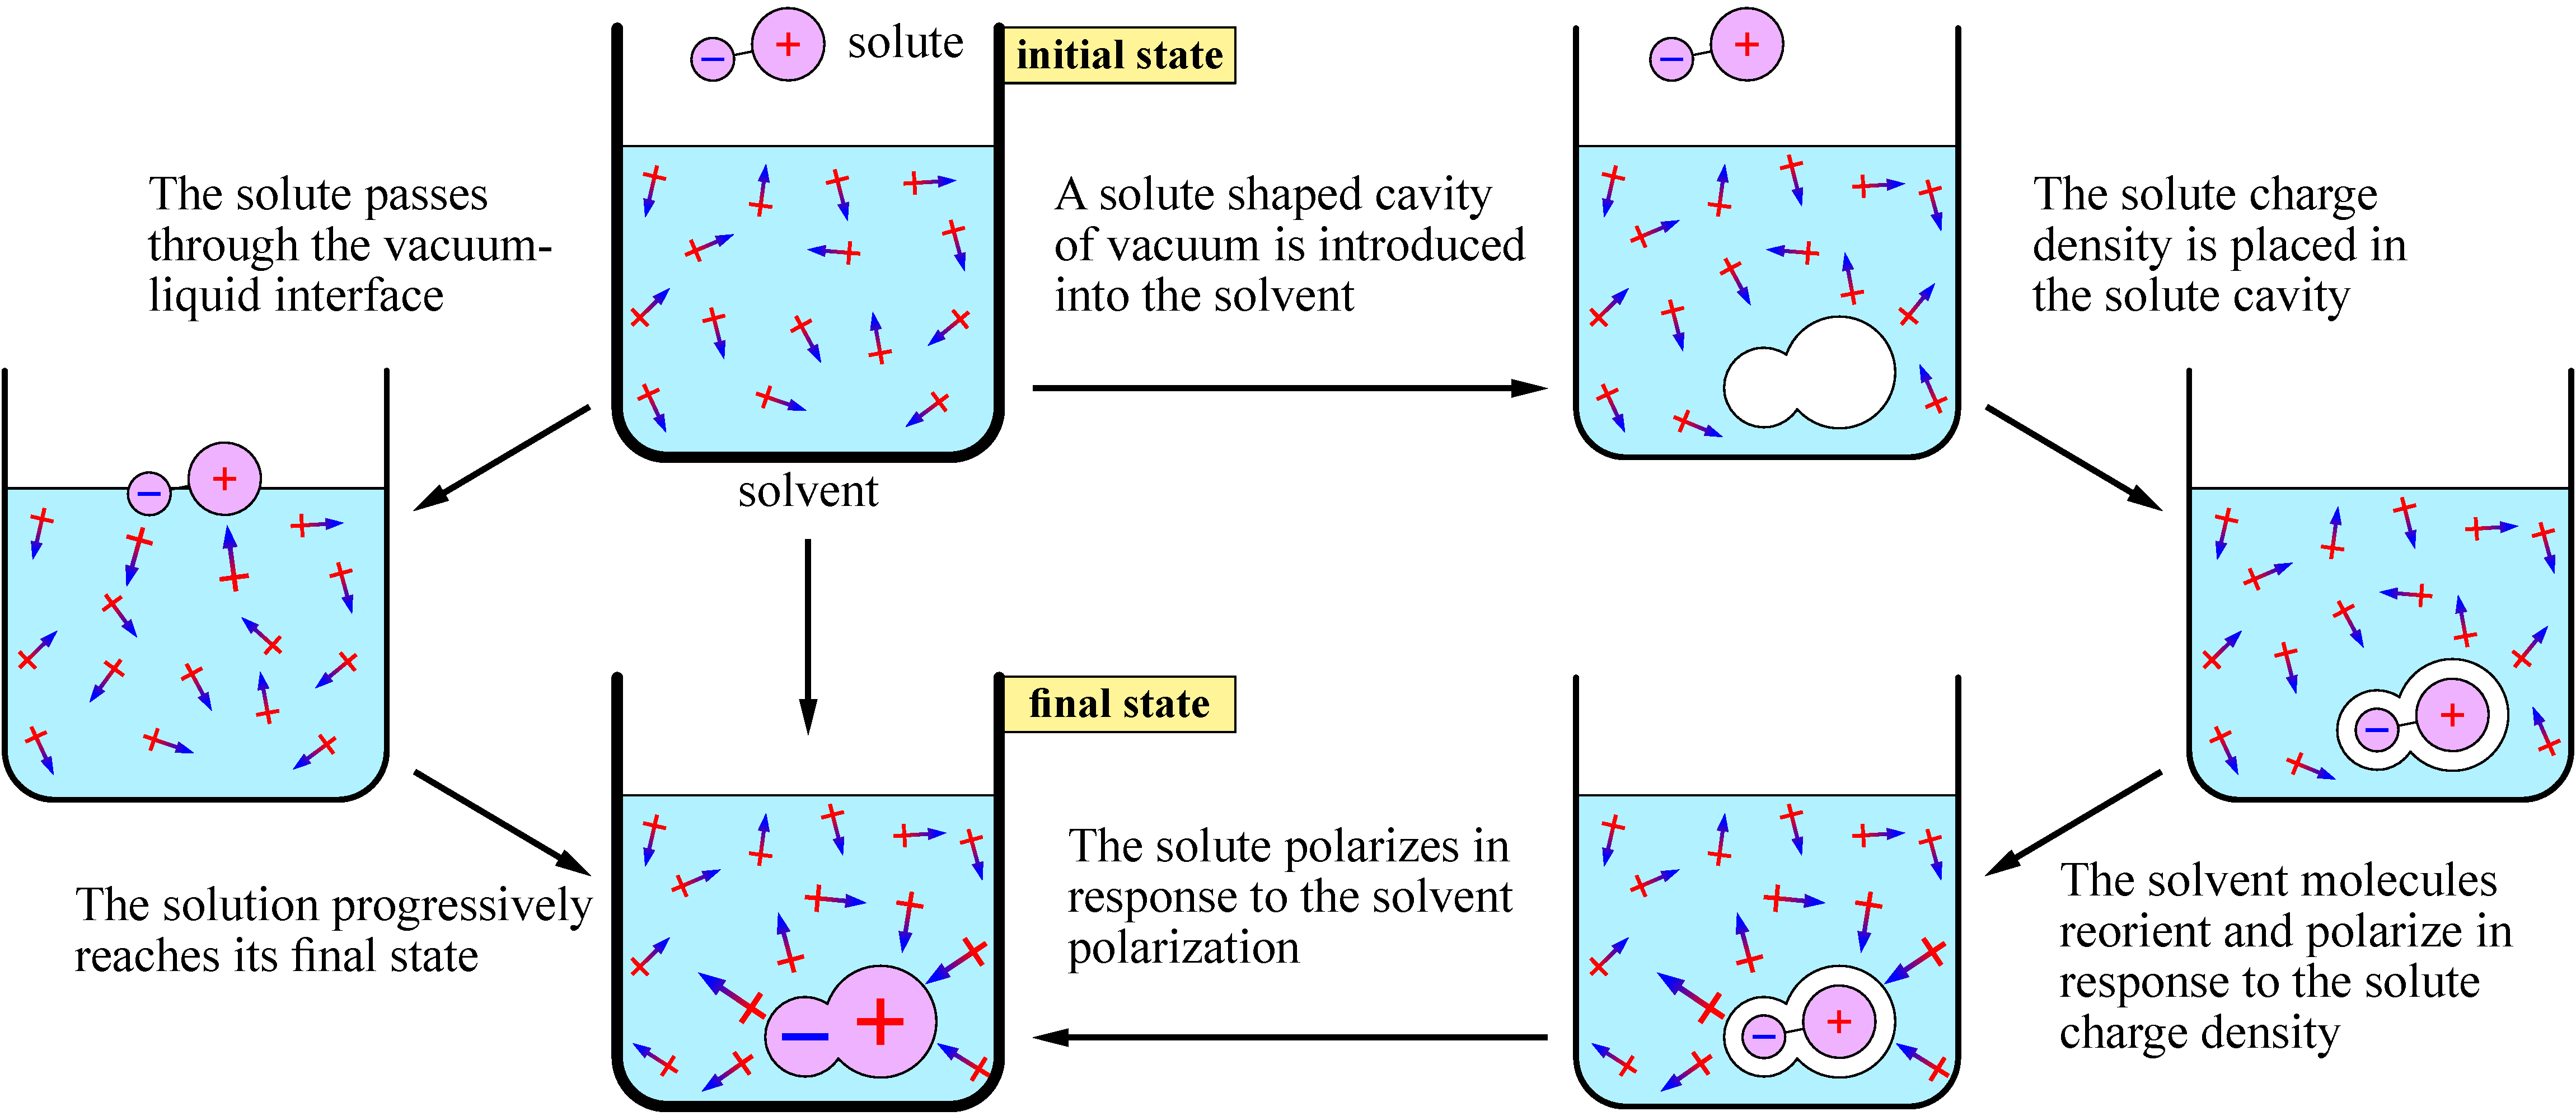
\includegraphics[width=1\columnwidth]{_figure/solvation}\caption[The solvation process]{The solvation process.\label{fig:Process-of-solvation} A thermodynamic
system, whose properties only depend on the initial and final states,
can go through different paths. The physical process of solvation
(left path) takes the solute from vacuum into bulk solvent, progressively
passing through the vacuum-liquid interface. Theoretically, the solvation
energy is defined as the energy consumed in such a process. In theoretical
studies, the process can be decomposed to some artificial unphysical
process (right path), involving the growth of an uncharged solute-sized
cavity within the bulk solvent, the transfer of the solute charge
distribution from vacuum into cavity, and the interaction between
the solute and solvent.}

\par\end{center}%
\end{minipage}
\end{figure}


To change a phenomenon to a model, we must first understand its process.
Solvation is defined as the process of moving a molecule from the
gas phase (or vacuum) to a condensed phase (figure \ref{fig:Process-of-solvation}),
which builds a stabilizing interaction with the solute (or solute
moiety like protein residues, interfaces, etc.) \citep{iupac}. Such
interactions are mostly classical, involving electrostatic
and van der Waals forces, with additional more specific chemical effects
such as hydrogen bond formation, and quantic effects for some small
solvents whose vibrational or rotational energy states are at the same
magnitude as $k_{\mathrm{B}}T$, etc. \citep{Gray-Gubbins}.

As not all kinds of interactions are important in applications, according
to the usage, different models and methods have been developed.

For most of the 20th century \citep{Cramer_1999}, the study of
solvation effects has been dominated by continuum (implicit) models,
which depend upon the dielectric constants and are not costly
in terms of computation resources. They provide an accurate way to treat the
strong, long-range electrostatic interactions which dominate many
solvation phenomena, but lack detailed information on the first
solvation shell. The latter, which mainly includes the cavity formation
energy and solute-solvent van der Waals interactions, is often rudely
treated by introducing an artificial form of cavity that links to the
form of solute. The methods for testing electrostatic interactions include
generalized Born model, or for better estimates via Poisson-Boltzmann
calculations. They are widely integrated within \acs{QM} simulations
of the solvent, by add extra solvation terms onto the Fock or Kohn-Sham
operator \citep{Jensen,scrf,Tomasi_1994_implicit_model}. However,
the improper treatment of the first-shell, where the microscopic interactions
are primarily located, often introduce sometimes huge error in free
energy evaluation, especially for polar solvents (like water), despite
the accuracy that the \acs{QM} calculation alone can achieve. Therefore,
classical molecular simulations, which describing the individual solvent
molecules (explicit), particularly the molecular dynamics (\acs{MD})
and Monte Carlo method (\acs{MC}), became the alternative solution
during the last few decades. They generate trajectories and configurations,
then estimate free energy changes by statistical mechanic technics,
such as free energy perturbation (FEP) theory or thermodynamic integration
(TI) \citep{Jorgensen_1995_MC}. These calculation is very demanding
on computing cost, due to the requirement of many (hundreds or thousands
of) solvent molecules to form a realistic model.

Recently, a third domain of theory to describe solvent, based on the
statistical mechanics of fluid, is growing rapidly. It is generally
called liquid theory, involves mainly the integral equation theory
(\acs{IET}), and the classical density functional theory for liquids.
These approaches are cope to give the molecular nature of the first-shell,
but without calculate all the instantaneous micro-states with respect
to time, which can be integrated over positions and momentums theoretically.
Therefore, they are of magnitudes faster than those simulations by
micro-states.

The integral equation theory (\acs{IET}) is about solving the Ornstein-Zernike
(\acs{OZ}) equation with a specific closure equation \citep{Hensen-McDonald,Gray-Gubbins}.
It was firstly limited to so called ``simple liquid'' - a system
of spherical particles. A part, Chandler and Andersen in 1971 \citep{Chandler_1972_RISM}
developed the reference interaction site model (\acs{RISM}), which
discretizes the distribution and correlation functions into a site-site
set of functions, and solve the \acs{OZ} equation in matrix \citep{hirata_molecular_2004}.
Another part, Blum \citep{Blum_I,Blum_II}, Fries and Patey \citep{Fries_Patey_1985}
extend the \acs{OZ} equation to molecular case, where the distribution
and correlation functions depend on both position and orientation.
In their theory, the orientation part of \acs{OZ} equation is simplified
by expending the distribution and correlation functions on Wigner
generalized spherical harmonics.

The classical density functional theory approach deal with inhomogeneous
liquids, which uses the same variation principle and minimization
strategy \citep{mermin_thermal_1965,Evans_1979,Hansen_1987} as electronic
density functional theory \acs{DFT} that treats electric interactions
and has a great success in computational chemistry. It gives the Helmholtz
free energy and the equilibrium solvent density, by minimizing the
free energy functional of the solvent density in the presence of a
given external potential. Borgis and collaborators \textcolor{red}{{[}too
many ref{]}} have recently generalized it into molecular case, named
molecular density functional theory (\acs{MDFT}), where the solvent
density depends on both position and orientation, $\rho(\mathbf{r},\mathbf{\Omega})$.
The main theoretical difficulty lies in the definition of well-funded
and reliable functionals of the excess free energy $\mathcal{F}_{\mathrm{exc}}\left[\rho\right]$,
according to the geometric complexity of the solvent molecule. Some
recent researches have shown that it is cope with linear solvents
like acetonitrile, but still have little non-satisfaction with the
most complex solvent, i. e. water. \acs{MDFT} can be proved to be
mathematically equivalent to the two-component molecular \acs{IET}.

The majority of work of all these theories have been focused on water,
since it is one of the most difficult systems to model due to its
molecular geometry, ineligible multi-body interaction, quantum effect,
hydrogen bond, etc. The importance of including instantaneous polarization
in potential functions is also an issue \citep{polarisable_1,polarisable_2}.
However, since polarizable force fields are not yet in common use,
the simulations by micro-states and the liquid theory which feed on
force field also have their own limit, compared to the continuum model
which can be polarizable. The advantages and disadvantages of each
branch of theory are listed in table \ref{tab:Theories-of-solvation}.

\begin{table}[h]
\begin{centering}
\begin{tabular}{ccccc}
\toprule 
\tableheadline{Theory} & \tableheadline{Speed} & \tableheadline{Long-Range} & \tableheadline{First-Shell} & \tableheadline{Polarizable Solvent}\tabularnewline
\midrule
Continuum model & fast & yes & no & fully\tabularnewline
Simulation by time & costly & yes & yes & partially, very costly\tabularnewline
Liquid theory & fast & yes & yes & partially\tabularnewline
\bottomrule
\end{tabular}
\par\end{centering}

\caption{Theories of solvation simulation\label{tab:Theories-of-solvation}}
\end{table}


This thesis consists in the development of the \acs{MDFT}, focusing
on the generalization and algorithmic acceleration of the excess free
energy functional $\mathcal{F}_{\mathrm{exc}}$ evaluation under homogenous
reference fluid (\acs{HRF}) approximation, which will be discussed
in detail in later chapters. 


\section{Scope of this thesis}

Chapter I reviews a selection of models and methods to the solvent
effect. It includes the mainly used continuum model, the basic of
liquid theory, as well as its two frontier research domains, \acs{IET}
and \acs{MDFT}. The code structure of \acs{MDFT}, which all the
development in this thesis is based on, is also presented. There is
also a brief introduction to \acs{MD} and \acs{MC}, as well as the
generation of direct correlation function (\acs{DCF}) used in this
thesis by such methods. 

Chapter II presents all the theory developed and newly used in this
thesis. In this thesis, two algorithms of excess energy functional
evaluation are proposed, one is extension of the previous algorithm,
other is a new algorithm, that combines the molecular \acs{OZ} equation
treatment of angular part with MDFT. The output solvation properties
is mainly the two: free energy, and solvent structure.

Chapter III takes note of all the implementation result, that divided
into two aspects, the ``accuracy'', which involves comparisons between
algorithms, and with \acs{IET} and \acs{MD} results; and the ``efficiency'',
which evaluate the computing cost of the code, both in sequential
and parallelized version.

Chapter VI gives some application to ions and molecules.


\ctparttext{This chapter gives a brief review of all the basic concepts and previous
work that this thesis is based on.\\
\medskip{}
In section \ref{chpt:models}, we begin by introducing the frequent
models of solvent in a simulation, from the simplest implicit continuum
model to the most complex explicit one. The overview of these models
then helps to understand the choice of description scale used in our
study, as well as its limits.\\
\medskip{}
Once the model is chosen, all the theories become mathematical problems.
Section \ref{chpt:statistical-mechanics} reviews some basic concepts
of statistical mechanics for liquids (theory of liquids), which present
some brief formalisms deduced for an atomic solvent model. The following
section \ref{chpt:iem-mdft} gives the extension of the theory to
molecular solvent in two frontier approaches: the integral equation
theory (\acs{IET}), and the molecular density functional theory (\acs{MDFT})
that this thesis works upon. A clear mathematical equivalence between
these two theories is also presented, which gave us the idea to use
the expansion technics in \acs{IET} to serve \acs{MDFT}. \\
\medskip{}
Section \ref{chpt:mdft} gives a detailed presentation of the initial
code \acs{MDFT}, which the development in this thesis is based on.}

\part{State of the Art: Solvation, Models and Methods}


\chapter{Model of Solution System\label{chpt:models}}

Computing models of solvents are broadly divided into two types: those
treating the solvent as a continuous medium (implicit models) and
those describing the individual solvent molecules (explicit models).
In the continuum model, the solvent is characterized by the dielectric
constant $\varepsilon$ and contains an artificially shaped cavity.
The explicit models can have more specific microscopic scales. Within
the scope of classical mechanics, the most detailed (and thus the
most expensive) methods involve flexible and polarizable explicit
models, while in computational chemistry, less detailed models often
have wider usage (for example, the proteins are treated in the unity
of residues). As the theory of liquids was initially established for
spherical atom-like solvent particles, the model adopted by such a
theory is a rigid entity carrying distributed point charges, characterized
by their position and orientation, i. e. there is no internal movement
considered. This approximation has been proven reasonable \citep{Gray-Gubbins}.
There also exist models in which the scale lies somewhere between
the implicit and explicit models; for example, so-called coarse-grained
models, which gather groups of atoms into a single interaction site.

In this section, we will give a brief introduction of the implicit
model in order to facilitate later discussion on solvation free energy
corrections. We will then focus on the rigid solvent models and discuss
the limits of such approximations. The flexible and polarizable models
will also be briefly mentioned. 

\section{Continuum solvation models}

Continuum models \citep{Jensen,Cramer_1999,Tomasi_1994_implicit_model},
which are popular in QM calculations, consider the solvent as a uniform
polarizable medium with dielectric constant $\varepsilon$\marginpar{The dielectric constant $\varepsilon$ is the key parameter characterizing
the solvent. It is normally a constant value, but that can depend
on the distance from the solute $M$. (see $\mathsection$\ref{subsec:Poisson=002013Boltzmann-methods})}, with the solute $M$ placed in the cavity within this medium (figure
\ref{fig:Reaction-field-model}) 

\begin{figure}[h]
\begin{centering}
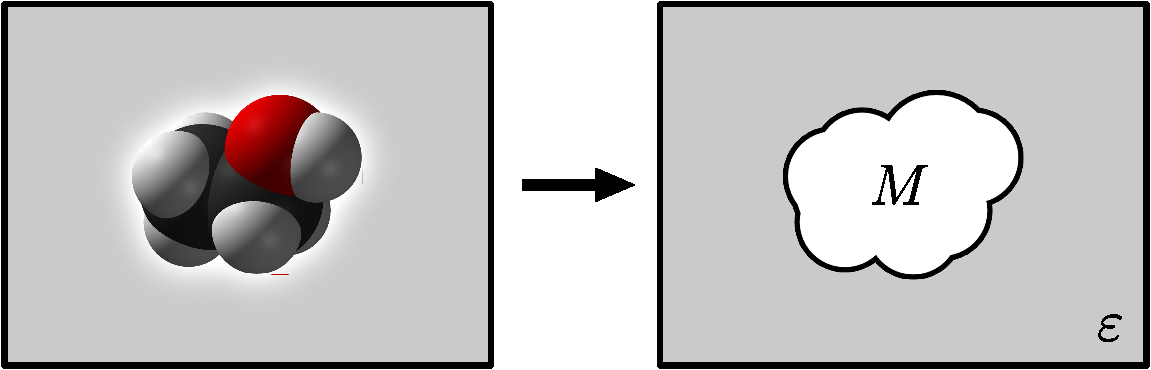
\includegraphics[width=0.72\columnwidth]{_figure/reaction-field-model_2}
\par\end{centering}
\caption{Continuum solvent model\label{fig:Reaction-field-model}}
\end{figure}

The solvation Gibbs free energy according to this model is
\begin{equation}
\Delta G_{\mathrm{solvation}}=\Delta G_{\mathrm{cavity}}+\Delta G_{\mathrm{dispersion}}+\Delta G_{\mathrm{elec}}\label{eq:cm}
\end{equation}
where $\Delta G_{\mathrm{cavity}}>0$ is the energy needed to create
a hole in the medium, and $\Delta G_{\mathrm{dispersion}}$ is the
dispersion interaction, which is roughly the van der Waals energy
$\Delta G_{\mathrm{vdW}}<0$ between the solvent and solute. In principle,
there may also be a repulsive component, and the dispersion term is
sometimes denoted dispersion/repulsion. $\Delta G_{\mathrm{elec}}<0$
is the contribution of electrostatic interactions, introduced by electric
charge distribution of $M$ which polarizes the medium, and the action
back of the medium on the molecule (reaction field). 

The initial two terms in eq. (\ref{eq:cm}) are linked to the configuration
of the first solvation shell (cavity). The definition of cavity varies
from the simplest sphere or ellipsoid to the ensemble of atomic surfaces
defined by the van der Waals radii in the solute. It is somewhat reasonable
to consider the cavity area as proportional to the number of solvent
molecules in the first solvation shell. This number can be calculated
as the area passing through the middle region of first shell solvent.
This area, named the solvent-accessible surface area (SASA) \citep{SAS_1,SAS_2},
can be calculated by adding the radius of the probe solvent ball on
the solvent excluded surface area (figure \ref{fig:sasa}).

\begin{figure}[h]
\begin{centering}
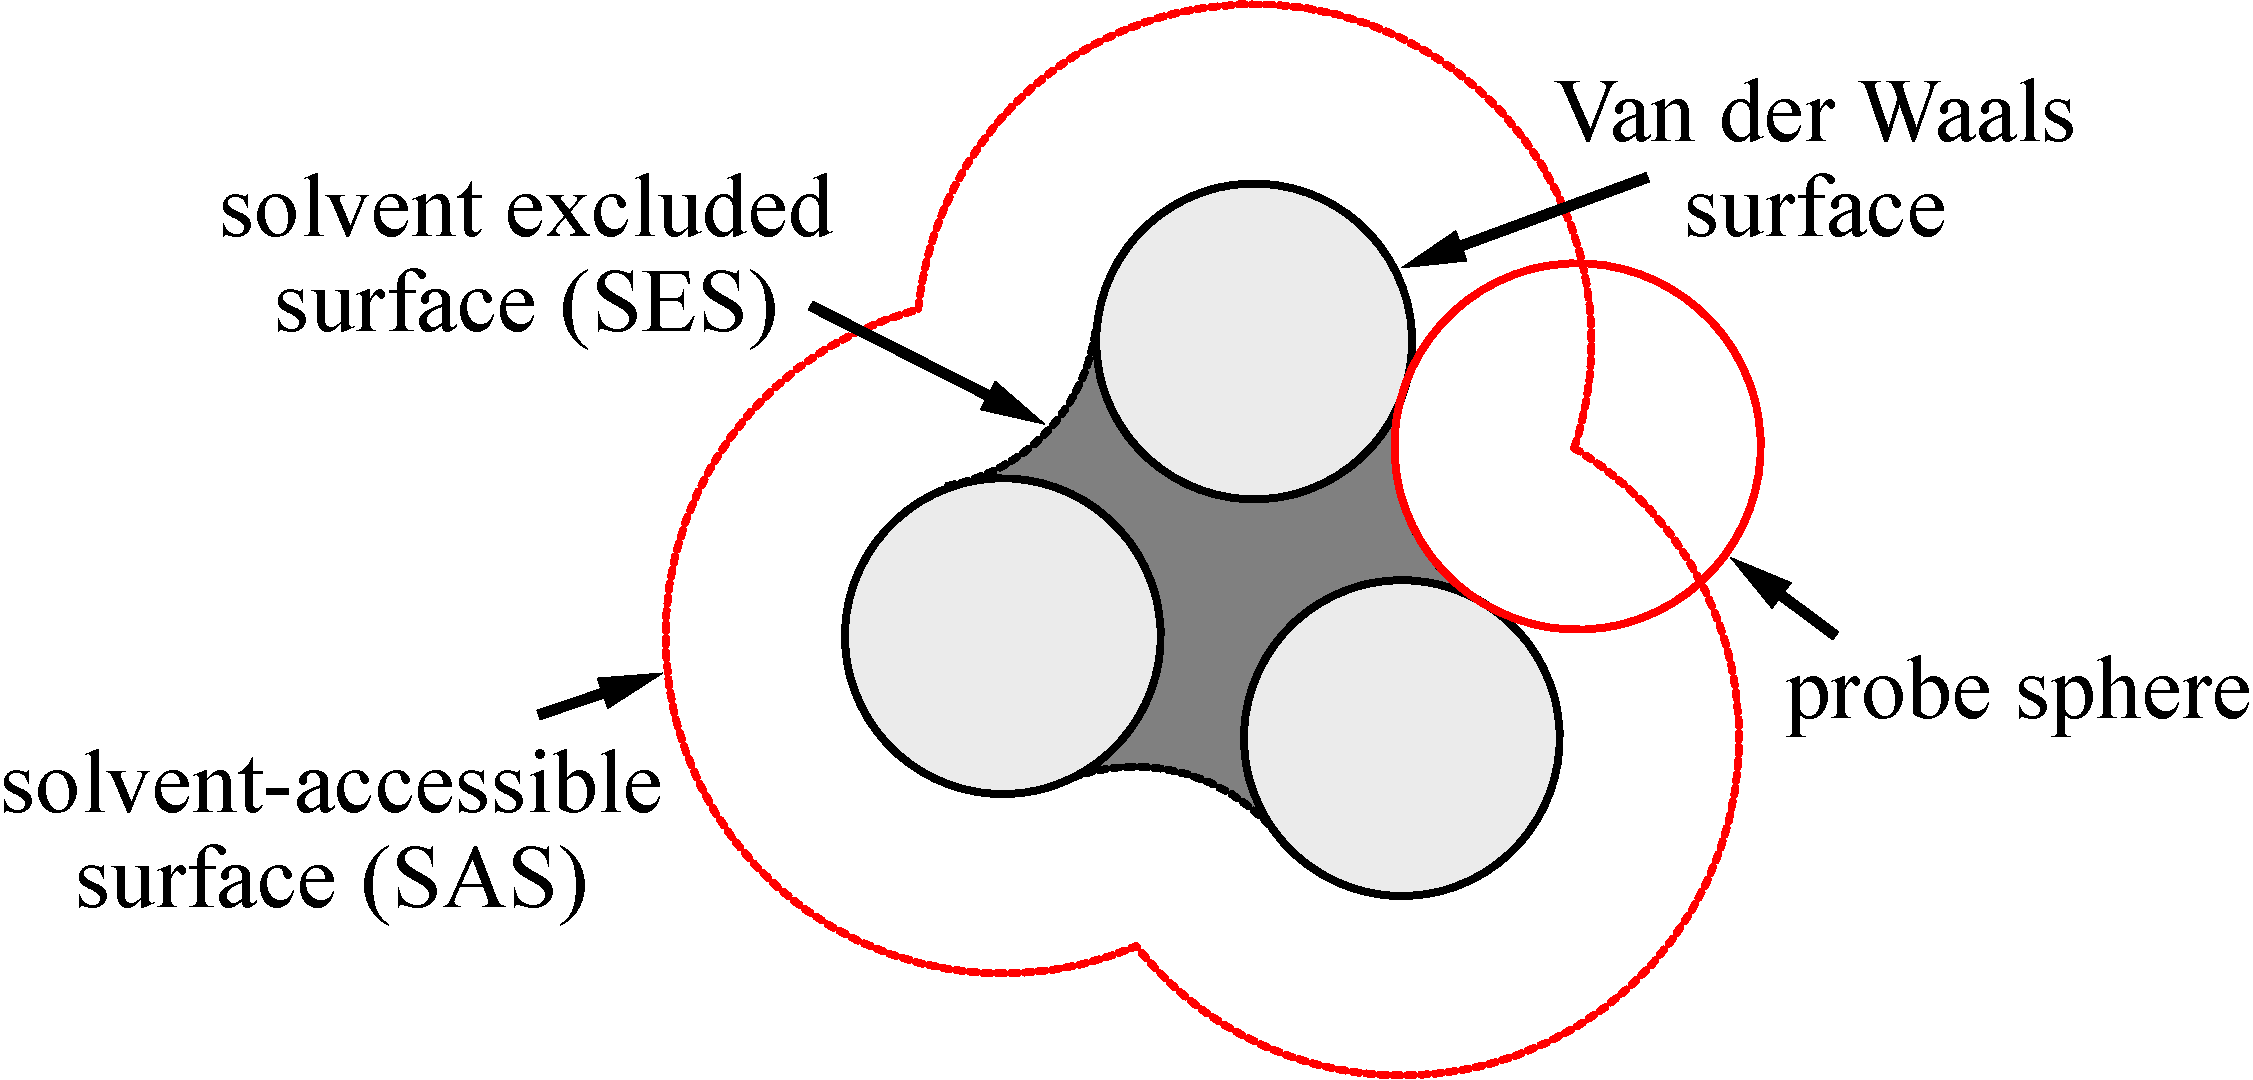
\includegraphics[width=0.55\columnwidth]{_figure/SASA}
\par\end{centering}
\caption[Definition of cavity surfaces]{Definition of cavity surfaces\label{fig:sasa}. The solvent accessible
surface (SAS) traced out by the center of the probe representing a
solvent molecule. The solvent excluded surface (SES) is the topological
boundary of the union of all possible probes that do not overlap with
the molecule.}
\end{figure}

The energy required to create such a cavity and the stabilization
due to van der Waals interactions between the solute and solvent,
assumed to be proportional to the surface area of the cavity, is expressed
as
\begin{equation}
\Delta G_{\mathrm{cavity}}+\Delta G_{\mathrm{dispersion}}=\gamma S_{\mathrm{SASA}}+\beta
\end{equation}
or parameterized by having a constant $\xi$ specific for each atom
type, with the $\xi$ parameters being determined by fitting to experimental
solvation data:
\begin{equation}
\Delta G_{\mathrm{cavity}}+\Delta G_{\mathrm{dispersion}}=\sum_{i}^{\mathrm{atoms}}\xi_{i}S_{i}
\end{equation}

The models and methods employed to calculate the electrostatic contribution
$\Delta G_{\mathrm{elec}}$ have varied greatly according to their
usage. The sections below list the most common examples. On another
topic, the integration of continuum models into \acs{QM} calculations
is also a very important field; these developments will not be detailed
here as they do not connect yet to our work. Such kinds of methods
are called the self-consistent reaction field (SCRF) models, which
integrate the calculation of the solute-solvent interaction in addition
to that of the solute wave function by an iterative procedure. Some
examples are presented in the list of Gaussian keyword SCRF \citep{scrf},
and the field is well reviewed by, for example, Tomasi \citep{Tomasi_1994_implicit_model,tomasi_quantum_2005}
and Jensen \citep{Jensen}.

\subsection{Poisson-Boltzmann methods\label{subsec:Poisson=002013Boltzmann-methods}}

The Poisson-Boltzmann equation (PBE) \citep{holst_1994_poisson} makes
it possible to calculate the position-dependent electrostatic potential
$V_{\mathrm{elec}}(\mathbf{r})$ in the continuum model, such that
the electrostatic component of the free energy can be written as
\begin{equation}
\Delta G_{\mathrm{elec}}=\frac{1}{2}\int\mathrm{d}\mathbf{r}\rho_{q}(\mathbf{r})V_{\mathrm{elec}}(\mathbf{r})
\end{equation}
where $\rho_{q}$ is the charge distribution \textcolor{red}{(of the
solute?).}

The Maxwell-Gauss equation in SI units convention gives
\begin{equation}
\nabla\cdot D(\mathbf{r})=\dfrac{\rho_{q}(\mathbf{r})}{\varepsilon_{0}}
\end{equation}
where $D(\mathbf{r})=\varepsilon_{0}E(\mathbf{r})+P(\mathbf{r})$
is the electric displacement field, $P(\mathbf{r})$ is the system
polarization, $E(\mathbf{r})$ the electric field, and $\varepsilon_{0}$
the vacuum permittivity. $D(\mathbf{r})$ can also be expressed in
terms of the position-dependent dielectric constant $\varepsilon(\mathbf{r})$,
$D(\mathbf{r})=\varepsilon(\mathbf{r})E(\mathbf{r})$, which thus
gives
\begin{equation}
\nabla\cdot\varepsilon(\mathbf{r})E(\mathbf{r})=\dfrac{\rho_{q}(\mathbf{r})}{\varepsilon_{0}}
\end{equation}
or in terms of electrostatic potential:
\begin{equation}
\nabla\cdot\left[\varepsilon(\mathbf{r})\nabla V_{\mathrm{elec}}(\mathbf{r})\right]=-\dfrac{\rho_{q}(\mathbf{r})}{\varepsilon_{0}}\label{eq:poisson}
\end{equation}

This second-order differential equation (\ref{eq:poisson}) is called
the Poisson equation. 

This equation cannot be solved analytically for complex geometries
(such as a protein). Therefore it is done numerically using appropriate
methods; for example, mentioned in the article of Roux and Simonson
\citep{roux_implicit_1999} or Holst \citep{holst_1994_poisson}.
A density functional approach based on the minimization of the polarization
density can also be used to solve this equation \citep{Marchi_2001,Levy_2005}.

If the solvent is ionic, the Poisson equation can be modified by taking
into account a (thermal) Boltzmann distribution of ions in the solvent,
i. e.,
\begin{equation}
\rho_{\mathrm{tot}}(\mathbf{r})=\rho_{q}(\mathbf{r})+qn_{\mathrm{ion}}\sinh(\frac{qe}{k_{\mathrm{B}}T}V_{\mathrm{elec}}(\mathbf{r}))
\end{equation}

for a salt composed of ions of charge $+q$ and $-q$ and of density
$n_{\mathrm{ion}}$. Replacing in eq. (\ref{eq:poisson}) leads to
the Poisson-Boltzmann Equation:
\begin{equation}
\nabla\cdot(\varepsilon(\mathbf{r})\nabla V_{\mathrm{elec}}(\mathbf{r}))-\dfrac{qn_{\mathrm{ion}}}{\varepsilon_{0}}\sinh\left(\dfrac{qV_{\mathrm{elec}}(\mathbf{r})}{kT}\right)=-\dfrac{\rho(\mathbf{r})}{\varepsilon_{0}}
\end{equation}


\subsection{Born / Onsager / Generalized Born models\label{subsec:Born-/-Onsager}}

For simple geometries, the Poisson equation (\ref{eq:poisson}) can
be solved analytically.

The simplest model is a spherical cavity. For a net charge $q$ in
a cavity of radius $a$, the electrostatic free energy of a medium
with a dielectric constant of $\varepsilon$ is given by the Born
formula:
\begin{equation}
\Delta G_{\mathrm{elec}}(q)=-\dfrac{1}{8\pi\varepsilon_{0}}\left(1-\frac{1}{\varepsilon}\right)\frac{q^{2}}{2a}
\end{equation}

Other similar models include the Onsager model, in which a point dipole
(characterized by the dipole moment $\mu$) is put in a spherical
cavity. The Kirkwood model refers to a general multipole expansion
in a spherical cavity, while the Kirkwood-Westheimer model arises
for an ellipsoidal cavity. Those simplified models are not fully able
to predict the solvent behavior in many realistic cases \citep{Jensen}. 

The generalized Born (GB) model is an empirical model based on the
superposition of several net charges in spherical cavities as the
Born model describes, with a similar formula:
\begin{equation}
\Delta G_{\mathrm{elec}}=-\dfrac{1}{8\pi\varepsilon_{0}}\left(1-\frac{1}{\varepsilon}\right)\sum_{i}\sum_{j}\frac{q_{i}q_{j}}{f_{ij}}
\end{equation}
where the function $f_{ij}$ depends on the internuclear distance
$r_{ij}$ between the centers of atoms $i$ and $j$ and on the Born
radii for each pair of atoms $a_{i}$ and $a_{j}$:
\begin{equation}
f_{ij}=\sqrt{r_{ij}^{2}-a_{i}a_{j}\exp\left(\frac{r_{ij}^{2}}{4a_{i}a_{j}}\right)}
\end{equation}

The key (empirical) point is to be able to attribute an effective
Born radius $a_{i}$ to each atom inside the complex, non-spherical
cavity formed by the solute. Once this is accomplished, the GB model
provides a very fast method, with an overall accuracy comparable to
that of Poisson-Boltzmann calculations. That makes it widely used
in computational structural biology to perform structure optimization
and molecular dynamics simulations.

\section{Model potential of explicit molecules}

The model potential frequently used in the theory of liquids is a
classical, rigid, pairwise additive model \citep{Hensen-McDonald,Gray-Gubbins}.
It is based on three assumptions. 
\begin{enumerate}
\item Firstly, the quantum effects should be ignored. It is assumed that
the rotational and transitional motion of solvent particles are continuous
and classical, which means the separation of both transitional and
rotational states are largely inferior of $k_{\mathrm{B}}T$. For
light molecules, that is not always convincing. Some molecules containing
hydrogen (e. g. $\mathrm{H_{2}O}$, $\mathrm{NH_{3}}$, and particularly
$\mathrm{H_{2}}$) exhibit obvious quantum effects at low temperature
in the liquid state. Gaseous $\mathrm{H_{2}O}$ and $\mathrm{NH_{3}}$
also need quantum effect corrections. However, for the liquid of most
interest to us, $\mathrm{H_{2}O}$ at room temperature, the contribution
of this effect is small enough to be neglected. And obviously, there
should not be any chemical interaction of the solvent with the solute.
\item Secondly,\marginpar{Compared to atomic models that only depend on $\mathbf{r}^{N}$, the
angular correlations can give influence on both structural and thermodynamic
proprieties. That is why our theory is extended to linear case ($\mathbf{\Omega}\equiv(\Theta,\Phi)$)
then molecular case ($\mathbf{\Omega}\equiv(\Theta,\Phi,\Psi)$ ).} the intramolecular movement (vibration and internal rotation) should
be either independent of transitional and rotational movement or absent.
This rigid molecule approximation assumes that the intermolecular
potential $\mathcal{U}(\mathbf{r}^{N},\mathbf{\Omega}^{N})$ for $N$
particles only depends on the positions of the $N$ molecular centers
$\mathbf{r}^{N}\equiv(\mathbf{r}_{1},\mathbf{r}_{2},\ldots,\mathbf{r}_{N})$
and on their orientations $\mathbf{\Omega}^{N}\equiv(\mathbf{\Omega}_{1},\mathbf{\Omega}_{2},\cdots,\mathbf{\Omega}_{N})$,
where $\mathbf{\Omega}\equiv(\Theta,\Phi,\Psi)$ represents the Euler
angles (figure \ref{fig:Euler-angles}). The natural choice for the
molecular center is the center of mass. This is, however, arbitrary
if only equilibrium properties are considered.

\begin{figure}[h]
\begin{centering}
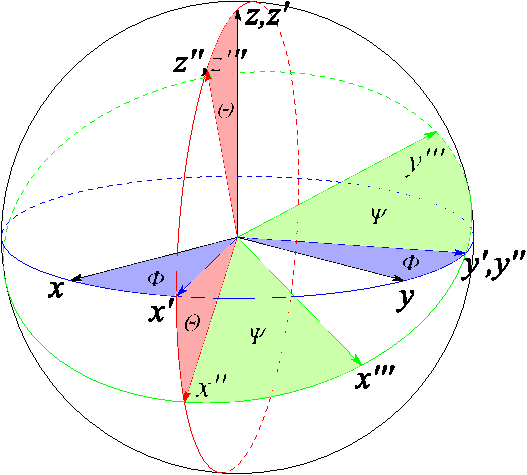
\includegraphics[scale=0.7]{_figure/euler_sphere}
\par\end{centering}
\caption[Euler angles]{Euler angles. The basis vectors of the new orientation are obtained
by 3 sequential operations: (1) A rotation $\phi$ $(0<\phi<2\pi)$
about the $z$-axis, bringing the frame of axes from the initial position
$\mathbf{S}$ into the position $\mathbf{S}'$ (2) A rotation $\theta$
$(0<\theta<\pi)$ about the $y$-axis of the frame $\mathbf{S}'$,
which is transformed into $\mathbf{S}''$ (3) A rotation $\psi$ $(0<\psi<2\pi)$
about the $z$-axis of the frame $\mathbf{S}''$.\label{fig:Euler-angles}}
\end{figure}

The rigid approximation is quite realistic for molecules in which
the separation of vibrational states largely exceeds $k_{\mathrm{B}}T$,
implying that the molecule stays in its ground vibrational state.
This is the case for many small solvent molecules such as $\mathrm{N_{2}}$,
$\mathrm{CO_{2}}$, $\mathrm{C_{6}H_{6}}$, and indeed for the bending
and stretching modes of water. 
\item Finally, the intermolecular forces have to be assumed as pairwise
additive:
\begin{equation}
\mathcal{U}(\mathbf{r}^{N},\mathbf{\Omega}^{N})=\frac{1}{2}\sum_{i\neq j}u(\mathbf{r}_{ij},\mathbf{\Omega_{i}},\mathbf{\Omega_{j}})=\sum_{i<j}u(\mathbf{r}_{ij},\mathbf{\Omega_{i}},\mathbf{\Omega_{j}})\label{eq:pair-potential}
\end{equation}
This means that the model potential only depends on the intermolecular
separation $\mathbf{r}$ and on the molecular orientations $\mathbf{\Omega}_{1}$
and $\mathbf{\Omega}_{2}$. This approximation is quasi-exact for
low density gases, where the contribution of the three and more body
terms decreases rapidly. But for dense fluids, in most of the cases
the multi-body potential cannot be ignored. The complete model potential
with higher-order corrections can be written in the form of
\begin{equation}
\mathcal{U}(\mathbf{r}^{N},\mathbf{\Omega}^{N})=\sum_{i<j}u(ij)+\sum_{i<j<k}u(ijk)+\sum_{i<j<k<l}u(ijkl)+...
\end{equation}
where $u(ij)=u(\mathbf{r}_{ij},\mathbf{\Omega_{i}},\mathbf{\Omega_{j}})$
and $u(ijk)=u(\mathbf{r}_{ij},\mathbf{r}_{jk},\mathbf{r}_{ki},\mathbf{\Omega_{i}},\mathbf{\Omega_{j}},\mathbf{\Omega_{k}})$,
etc. The omission of the three-body and higher-order terms can cause
error, for example, in surface tension and surface energy calculation
\citep{Miyazaki_1975}. However the higher-order terms are often accounted
for by an effective pair potential (measured by experiments or calculated
by simulations), which reduces considerably the computational cost
for simulations, or the degree of theory needed. Such models are presented
below going from simple to molecular liquids. For the molecular solvent
considered in this thesis, water, most publications have stayed at
this two-body level of description. 
\end{enumerate}

\subsection{Interaction of spherical particle}

The simplest model of a fluid is the hard sphere model. With $d$
the hard-sphere diameter, the pair potential is defined as:
\begin{equation}
u(r)=\begin{cases}
\infty & r<d\\
0 & r>d
\end{cases}
\end{equation}
This model is indeed a fundamental reference model in statistical
mechanics, and it can represent some physical systems, such as neutral
colloidal suspensions. However, the absence of attractive force, which
precludes the existence of a liquid-gas transition, makes it too simple
for realistic fluids. More realistic neutral particle models, like
the Lenard-Jones (LJ) model, exhibit a potential energy curve that
has the same shape as the real interaction of rare gas, as shown in
figure \ref{fig:LJ-pair-potential}.

\begin{figure}[h]
\begin{centering}
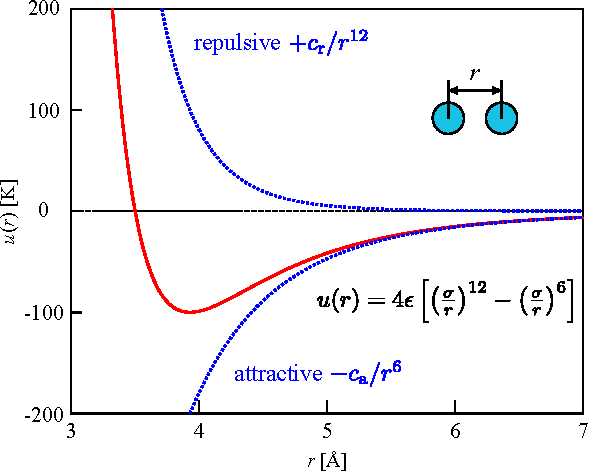
\includegraphics[scale=0.82]{_figure/lj-centre}
\par\end{centering}
\caption[LJ pair potential]{LJ pair potential. The plot gives the potential energy $u(r)$ versus
internuclear distance $r$ of two particles. At large distances, both
attractive and repulsive interactions are small. As the distance between
the atoms decreases, the attractive electron-proton interactions dominate,
and the energy of the system decreases. At the observed bond distance,
the repulsive electron-electron and proton-proton interactions just
balance the attractive interactions, preventing a further decrease
in the internuclear distance. At very short internuclear distances,
the repulsive interactions dominate, making the system less stable
than the isolated atoms.\label{fig:LJ-pair-potential}}
\end{figure}

The Lennard-Jones (LJ) interaction gives

\begin{equation}
u_{LJ}(r)=4\varepsilon\left[\left(\frac{\sigma}{r}\right)^{12}-\left(\frac{\sigma}{r}\right)^{6}\right]
\end{equation}
where $r$ is the distance from centre to centre, $\sigma$ is the
collision diameter or the particles separation where $u(r)=0$, and
$\epsilon$ is the well depth of the potential (of unity energy $\mathrm{kJ/mol}$).
The well minimum occurs at $r_{\min}=2^{1/6}\sigma$ and $u(r_{\min})=-\epsilon$.
The parameters $\sigma$ and $\epsilon$ can be extracted from experiments.

Theoretically, all terms in the multipole series represent attractive
contributions to the potential. The leading term, varying as $r^{-6}$,
describes the \textcolor{red}{(quantum?)} dipole-dipole interaction.
Higher-order terms represent dipole-quadrupole ($r^{-8}$), quadrupole-quadrupole
($r^{-10}$) interactions, and so on, but these are negligible compared
to $r^{-6}$. The short-range interaction is difficult to define properly,
and for the sake of simplicity and numerical efficiency, it is defined
as $r^{-12}$ in the LJ model. 

If the spherical particles are charged (as in molten salts), the electrostatic
interaction between them is described by the Coulomb point charge
interaction:
\begin{equation}
u_{\mathrm{Coul}}(r)=\frac{q_{1}q_{2}}{4\pi\varepsilon_{0}r}
\end{equation}

For such charged simple fluids, the overall pair $u(r)$ is a sum
of LJ and Coulomb interactions. Such \textcolor{red}{decomposition}
can be extended to molecular fluids in terms of site-site interactions,
which are discussed in the following section.

\subsection{Site-site interactions}

Indeed, a spherical description of interactions is not sufficient
to fully describe molecular fluids. The site-site model is a further
extension of atomic models, in which the solvent molecule is represented
by a set of discrete interaction sites. The total potential energy
is a sum of spherical interaction potentials:
\begin{equation}
u(1,2)=\frac{1}{2}\sum_{\alpha}\sum_{\beta}u_{\alpha\beta}(\left|\mathbf{r}_{2\beta}-\mathbf{r}_{1\alpha}\right|)
\end{equation}
\textcolor{red}{(the $1/2$ ?) }where $\mathbf{r}_{is}$ is the coordinates
of site $s$ in molecule $i$, $u_{\alpha\beta}(r)$ the interatomic
potential energy of pairs of sites $\alpha$ and $\beta$, as discussed
above. More specifically, it is generally decomposed into a Lennard-Jones
and a Coulombic contribution:
\begin{equation}
u(1,2)=\frac{1}{2}\sum_{\alpha}\sum_{\beta}\left\{ 4\epsilon_{\alpha\beta}\left[\left(\frac{\sigma_{\alpha\beta}}{r_{12}^{\alpha\beta}}\right)^{12}-\left(\frac{\sigma_{\alpha\beta}}{r_{12}^{\alpha\beta}}\right)^{6}\right]\:+\frac{1}{4\pi\varepsilon_{0}}\frac{q_{\alpha}q_{\beta}}{r_{12}^{\alpha\beta}}\right\} 
\end{equation}
where $r_{12}^{\alpha\beta}=\left|\mathbf{r}_{2\beta}-\mathbf{r}_{1\alpha}\right|$,
$\epsilon_{\alpha\beta}$ and $\sigma_{\alpha\beta}$ are the site-site
LJ parameters and $q_{\alpha}$ the partial charge on each site. This
model is the most commonly adopted, and it will be so in this thesis.

\subsection{Multipole and spherical harmonic expansion}

To obtain fewer terms in the calculation, the model potential can
be presented in convergent series via multipole or spherical harmonic
expansion.

For polar liquids, the dipole-dipole interaction should be mainly
taken into account. Thus the model considers dipole-dipole interactions
in addition to a spherically symmetric Lennard-Jones-like potential:
\begin{equation}
u(1,2)=u_{0}(r)-\boldsymbol{\mu}_{1}\cdot\mathbf{T}(\mathbf{r})\cdot\boldsymbol{\mu}_{2}
\end{equation}
where $\mathbf{r}$ is the vector separation of the molecular centers,
$u_{0}(r)$ is the spherically symmetric term discussed above, $\boldsymbol{\mu}_{i}$
is the dipole moment vector of particle $i$ and $\mathbf{T}(\mathbf{r})$
is the dipole-dipole interaction tensor:
\begin{equation}
T(\mathbf{r})=\nabla^{2}\left(\dfrac{1}{r}\right)=3\mathbf{r}\mathbf{r}/r^{5}-\mathbf{I}/r^{3}
\end{equation}
and $\mathbf{I}$ is the unit tensor. Note that this model can be
made more realistic by including higher-order electrostatic interactions,
such as dipole-quadrupole, quadrupole-quadrupole, etc. Such a systematic
multipolar approach has been proposed for water \citep{Chowdhuri_2006}.

Alternatively, the intermolecular potential can be expanded onto rotational
invariants in the form:
\begin{equation}
u(\mathbf{r}_{12},\mathbf{\Omega}_{1},\mathbf{\Omega}_{2})=\sum_{mnl\mu\nu}u_{\mu\nu}^{mnl}(r_{12})\Phi_{\mu\nu}^{mnl}(\hat{\mathbf{r}}_{12},\mathbf{\Omega}_{1},\mathbf{\Omega}_{2})
\end{equation}
where the angular basis functions $\Phi_{\mu\nu}^{mnl}(\hat{\mathbf{r}}_{12},\mathbf{\Omega}_{1},\mathbf{\Omega}_{2})$
can be expressed in terms of generalized spherical harmonics (\acs{GSH}s)
\citep{Gray-Gubbins}. A detailed description of rotational invariant
transform is in appendix \ref{chpt:rotational-invariant-expansion}.

\subsection{SPC/E water model}

As water cannot be perfectly described by a pair potential (due to
multi-body effects, quantum effects, hydrogen bond, etc.), various
models have been developed to fit a maximum number of properties.
Those models contain several sites, which can be placed possibly elsewhere
than at the center of atoms (figure \ref{fig:Water-models}). The
more sites the model has, the more precise it can be. There is a great
work done by Martin Chaplin \citep{water-model} to summarize the
most widely used water models.

\begin{figure}[h]
\begin{centering}
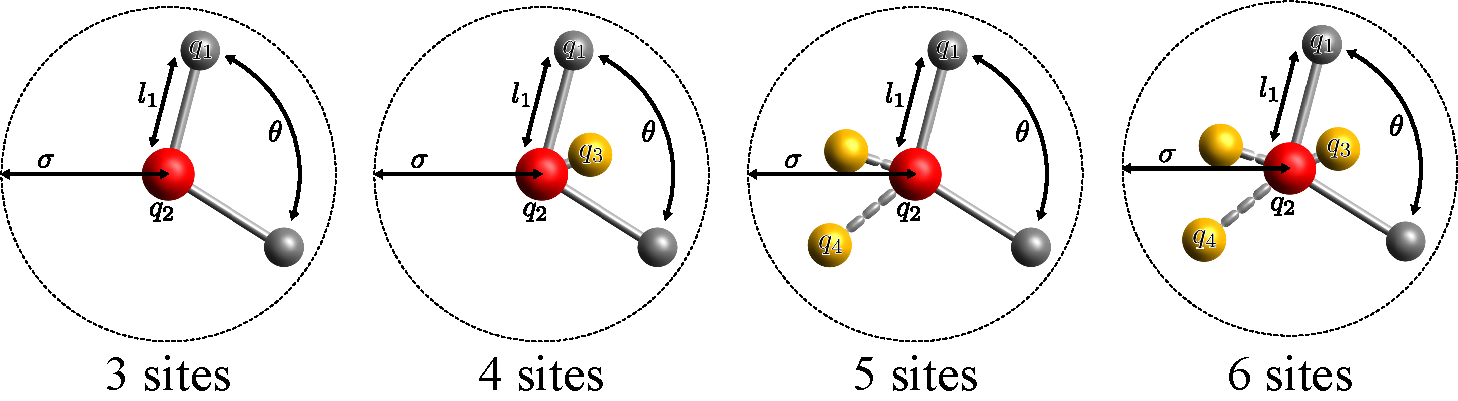
\includegraphics[width=0.75\columnwidth]{_figure/water}
\par\end{centering}
\caption{Water models\label{fig:Water-models}}
\end{figure}

In this thesis, we use the extended simple point charge model (SPC/E)
of water \citep{SPC/E} as our solvent model through all this thesis.
\marginpar{It should be noted that any rigid solvent model is compatible with
the theory of liquids, e. g. acetonitrile used in \citep{Zhao_2011}.} It is a 3-site model, the electrostatic interaction being modeled
using Coulomb's Law and the dispersion and repulsion forces using
the Lennard-Jones potential, as described above.

With respect to the original SPC model, the SPC/E model adds a polarization
correction term to the SPC potential energy in order to better match
the experiment:

\[
E_{\mathrm{pol}}=\frac{1}{2}\sum_{i}\dfrac{(\mu-\mu^{0})^{2}}{\alpha_{i}}
\]
where $\mu$ is the dipole of the effective pair model, $\mu^{0}$
is the dipole moment of an isolated water molecule, and $\alpha_{i}$
is the isotropic scalar polarizability \citep{SPC/E}. The SPC/E model
gives a better radial distribution function and diffusion constant
than the SPC model. It is the most commonly used model for applications.

Some parameters are listed in table \ref{tab:SPC/E}, compared with
its relative SPC model.

\begin{table}[h]
\subfloat[Structural parameters ]{\begin{centering}
\begin{tabular*}{1\columnwidth}{@{\extracolsep{\fill}}lllllll}
\toprule 
\tableheadline{Model} & $\sigma$ $[\lyxmathsym{\AA}^{6}]$ & $\varepsilon$ $[\mathrm{kJ\cdot mol^{-1}}]$ & $l_{1}$ $[\text{\AA}]$ & $q_{1}$ $[e]$ & $q_{2}$ $[e]$ & $\theta$ $[\text{\textdegree}]$\tabularnewline
\midrule
SPC \citep{spc} & 3.166 & 0.650 & 1.0000 & +0.410 & -0.8200 & 109.47\tabularnewline
SPC/E \citep{SPC/E} & 3.166 & 0.650 & 1.0000 & +0.4238 & -0.8476 & 109.47\tabularnewline
\midrule 
experiment \citep{water_exp} & - & - & 0.991 & - & - & 105.5\tabularnewline
\bottomrule
\end{tabular*}
\par\end{centering}
}

\subfloat[Calculated physical properties. All the data is at 25 \textdegree C
and 1 atm.]{\begin{centering}
\begin{tabular*}{1\columnwidth}{@{\extracolsep{\fill}}lllll}
\toprule 
\tableheadline{Model} & \tableheadline{{\footnotesize{}Molar}} & \tableheadline{{\footnotesize{}Number} } & \tableheadline{{\footnotesize{}Dielectric}} & \tableheadline{{\footnotesize{}Dipole}}\tabularnewline
 & \tableheadline{{\footnotesize{}Volume {[}$\mathrm{cm^{3}}${]}}} & \tableheadline{{\footnotesize{}Density}} & \tableheadline{{\footnotesize{}Constant}} & \tableheadline{{\footnotesize{}Moment {[}D{]}}}\tabularnewline
\midrule
SPC &  &  & 65 \citep{spc_dc} & 2.274\citep{SPC/E}\tabularnewline
SPC/E &  & \textcolor{red}{{[}ref? unity?{]}} & 71 \citep{Kusalik_1994_dc_spc/e,SPC/E} & 2.351\citep{SPC/E}\tabularnewline
\midrule 
experiment & 18.0685 {[}1006{]} &  & 78.4 & 2.95\tabularnewline
\bottomrule
\end{tabular*}
\par\end{centering}
}\caption{Parameters for SPC and SPC/E water\label{tab:SPC/E}}
\end{table}


\subsection{Flexible and polarizable models}

Up to this point, molecules were considered as rigid bodies. Flexible
models give extra degrees of freedom in vibration and internal rotation.
In that case, the interaction potential contains several extra terms,
yielding typically five kinds of forces: three for the direct interactions
in addition to the two indirect interactions (LJ and Coulomb).

\begin{figure}[h]
\begin{centering}
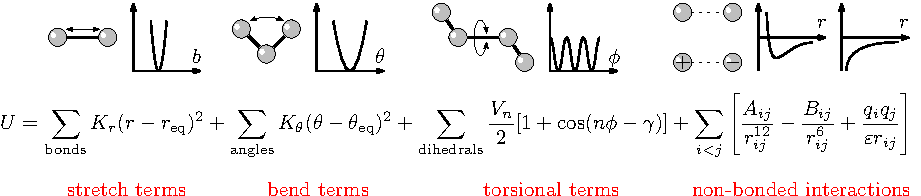
\includegraphics[width=1\columnwidth]{_figure/flexible}
\par\end{centering}
\caption{Interactions in a flexible model}
\end{figure}

The flexible yielding can deal with the non-rigidity of the solvent,
which is partially polarized owing to the vibrational degrees of freedom
(the so-called atomic polarizability). On the other hand, electronic
polarizability (the deformation of the molecule electron cloud under
the action of the external electric field) can be taken into account
even in a rigid model. This polarizability can be described by introducing
a modifiable charge distribution, for example by adding an induced
dipole at the molecular center of the molecule, or even on each of
its atomic sites, and by solving the set of induced dipoles self-consistently.
Introducing variable atomic charges is possible too \textcolor{red}{{[}ref{]}}.
Optimizing the induced charges/dipoles has a large computational overhead
compared to fixed charges.

Complex models require expensive computing cost, but still can have
large fluctuations due to use of imposed small system size. There
is a compromise between the choice of model and the choice of system
size. For this reason, the rigid models are still nowadays the most
popular. On the other hand, computing technologies have greatly developed
compared to the theories themselves, which makes it possible to use
more and more precise models in computation. 

\section{Model of solute}

The model of solute also have a substantial influence on the predicted
energy and structure of solvation. The solute can eventually be treated
by \acs{QM} calculations in terms of wave function and electron density.
This is the case for the implicit SCRF method, which for apolar solvents
(i.e. toluene) has been proven to work well. There is a clear mismatch
, however, between the very refined description of the solute and
the rather primitive continuous-medium treatment of the solvent. The
compromise to have a better model of solvent or solute is debatable,
and should vary according to the applications. On the other extreme,
one never uses a quantum solvent model with an implicit solute; this
would not be profitable even if the solute is of simple geometry (wall).
In the case of molecular solutes, it is consistent to require the
solute and solvent to have at least the same scale of description.
Within molecular force fields, this leads to the hierarchy of potential
models described in figure (\ref{fig:Hierarchy-of-models}).
\begin{figure}[h]
\centering{}%
\noindent\begin{minipage}[t]{1\columnwidth}%
\begin{center}
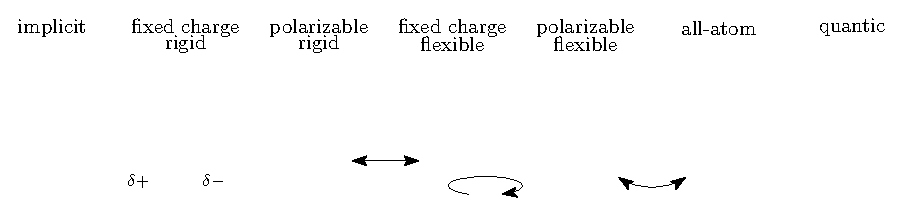
\includegraphics[width=1\columnwidth]{_figure/solute}
\par\end{center}%
\end{minipage}\caption{Hierarchy of models\label{fig:Hierarchy-of-models}}
\end{figure}

In this thesis, our first step will be to use a rigid molecular model
to describe the solute. This is coherent with IET, which cannot treat
the solvent and solute at different scales of description. Polarizable
and/or flexible models of solute, and the coupling of a QM solute
to the molecular solvent, will be described in perspective.

In conclusion, the choice of model for the solute/solvent system is
a compromise between the required precision according to the application,
and the computing cost that the research can afford.



\chapter{Statistical Mechanics of Classical Fluids \label{chpt:statistical-mechanics}}

The link between statistical mechanics and thermodynamics

From pair distribution functions and interaction potential, we can
derive information about solvent equilibrium state.

equilibrium statistical mechanics of classical fluids.

one component bulk fluids. thermodynamic state point is specified
by $\rho$ and temperature T. 


\section{Hamiltonian of a micro-state}

effective Hamiltonian, i.e. the theorist constructs a model fluid. 

In classical mechanics, the instantaneous state (phase point) of a
$N$-particle solvent system is specified by $3N$ coordinates $\mathbf{r}^{N}\equiv\mathbf{r}_{1},\ldots,\mathbf{r}_{N}$
and $3N$ moments $\mathbf{p}^{N}\equiv\mathbf{p}_{1},\ldots,\mathbf{p}_{N}$.
The Hamiltonian of the system is

\begin{equation}
H_{N}(\mathbf{r}^{N},\mathbf{p}^{N})=K_{N}(\mathbf{p}^{N})+V_{N}(\mathbf{r}^{N})+V_{N}^{\mathrm{ext}}(\mathbf{r}^{N})
\end{equation}
where

\begin{tabular}{ll}
$K_{N}(\mathbf{p}^{N})$ & $={\displaystyle \sum_{i=1}^{N}\frac{\mathbf{p}_{i}^{2}}{2m}}$ is
the kinetic energy \tabularnewline
$V_{N}(\mathbf{r}^{N})$ & $={\displaystyle \sum_{i<j}^{N}u(\left|\mathbf{r}_{i}-\mathbf{r}_{j}\right|)+3\,\mathrm{body}+\ldots}$
is the interatomic potential energy $\mathcal{U}(\mathbf{r}^{N})$.
One then has a pairwise additive description of the total inter-particle
potential, which leads us to define a model or effective Hamiltonian
as\tabularnewline
$V_{N}^{\mathrm{ext}}(\mathbf{r}^{N})$ & $={\displaystyle \sum_{i=1}^{N}}V_{\mathrm{ext}}(\mathbf{r}_{i})$
is the potential energy arising from the interaction of the particles
with the external field\tabularnewline
 & \tabularnewline
\end{tabular}.

The distribution of phase points of systems in \textcolor{red}{the
ensemble} is described by a phase space probability density $f^{[N]}(\mathbf{r}^{N},\mathbf{p}^{N};t)$,
such that 
\begin{equation}
\int f^{[N]}(\mathbf{r}^{N},\mathbf{p}^{N};t)\mathrm{d}\mathbf{r}^{N}\mathrm{d}\mathbf{p}^{N}=1
\end{equation}
for all $t$.

subset of particles of size $n$, reduced phase space distribution
function 
\begin{equation}
f^{[n]}(\mathbf{r}^{n},\mathbf{p}^{n};t)=\dfrac{N!}{(N-n)!}\int f^{[N]}(\mathbf{r}^{N},\mathbf{p}^{N};t)\mathrm{d}\mathbf{r}^{N-n}\mathrm{d}\mathbf{p}^{N-n}=1
\end{equation}
where $\mathbf{r}^{n}\equiv\mathbf{r}_{1},\ldots,\mathbf{r}_{n}$
and $\mathbf{r}^{N-n}\equiv\mathbf{r}_{n+1},\ldots,\mathbf{r}_{N}$.
The probability of finding a subset of $n$ particles in the reduced
phase space element.... the factor is the number of ways one can choose
a subset of size $n$.

The Liouville theorem shows that the probability density is independent
of time.

The Bogoliubov–Born–Green–Kirkwood–Yvon hierarchy express $f^{(n)}$
in terms of $f^{(n+1)}$, approximation closure


\section{Time averages and ensemble averages / Partition functions and Thermodynamics}

The classical canonical partition function for a one component fluid
is given by:
\begin{equation}
Z_{N}(\beta,V)=\dfrac{h^{-dN}}{N!}\int\mathrm{d}\mathbf{r}^{N}\mathrm{d}\mathbf{p}^{N}e^{-\beta H_{N}}
\end{equation}
$d$ is the dimensionality and $V$ is the volume of the system. We
can integrate over the moments to obtain
\begin{equation}
Z_{N}(\beta,V)=\Lambda^{-dN}Q_{N}
\end{equation}
\begin{equation}
Q_{N}=\dfrac{1}{N!}\int\mathrm{d}\mathbf{r}^{N}e^{-\beta\mathcal{U}(\mathbf{r}_{1},\ldots,\mathbf{r}_{n})}
\end{equation}
is the configurational partition function. Note that the potential
energy $\mathcal{U}(\mathbf{r}_{1},\ldots,\mathbf{r}_{n})$ may still
include an external field contribution.

The Helmholtz free energy is simply

\[
F_{N}(\beta,V)=-\beta^{-1}\ln Z_{N}
\]
which leads to entropy 
\[
S=\left(\dfrac{\partial F_{N}}{\partial T}\right)_{V}
\]
pressure
\[
p=\left(\dfrac{\partial F_{N}}{\partial V}\right)_{T}
\]
for bulk fluid

For an ideal (non-interacting) gas, where $\Phi\rightarrow0$, in
$d=3$???
\[
\beta F_{N}=\ln(N!\Lambda^{3N}V^{-N})=N\ln(\Lambda^{3}\rho)-N
\]
Stering equation... number density $\rho=N/V$ (a uniform ideal classical
gas.)

The grand function We consider open systems with fixed temperature
$T$ and chemical potential $\mu$. The partition function for the
grand canonical ensemble is

\begin{equation}
\Xi(\beta???,\mu,T)=\sum_{N=0}^{\infty}\frac{e^{\beta\mu N}}{h^{3N}N!}\iint\mathrm{d}\mathbf{r}^{N}\mathrm{d}\mathbf{p}^{N}e^{-\beta H_{N}(\mathbf{r}^{N},\mathbf{p}^{N})}=\sum_{N=0}^{\infty}\frac{1}{N!}\int\mathrm{d}\mathbf{r}^{N}e^{-\beta V_{N}(\mathbf{r}^{N})}\left(\prod_{i=1}^{N}\frac{e^{\beta u(\mathbf{r}_{i})}}{\Lambda^{3N}}\right)
\end{equation}
with $\Lambda=(2\pi\hbar^{2}/m)^{\frac{1}{2}}$ and $u(\mathbf{r})=\mu-V_{\mathrm{ext}}(\mathbf{r})$.

The equilibrium density of probability 
\[
f(\mathbf{r}^{N},\mathbf{p}^{N};N)=\frac{1}{h^{3N}N!}\frac{1}{\Xi}e^{-\beta\left[H_{N}(\mathbf{r}^{N},\mathbf{p}^{N})-\mu N\right]}
\]


and the grand potential

\[
\Omega=-\beta^{-1}\ln\Xi(\beta???,\mu,T)
\]


which for the case of a uniform fluid, reduces to $\Omega=-pV$ . 

\[
\Omega\left[u\right]=\beta^{-1}\left\langle \ln\left(h^{3N}N!f(\mathbf{r}^{N},\mathbf{p}^{N};N)\right)+K_{N}(\mathbf{p}^{N})+V_{N}(\mathbf{r}^{N})-\sum_{i=0}^{N}u(\mathbf{r}_{i})\right\rangle 
\]


\[
u(\mathbf{r}_{i})=\int\delta(\mathbf{r}-\mathbf{r}_{i})u(\mathbf{r})\mathrm{d}\mathbf{r}
\]


\[
\rho(\mathbf{r})=\left\langle \sum_{i=1}^{N}\delta(\mathbf{r}-\mathbf{r}_{i})\right\rangle 
\]


\[
\Omega\left[u\right]=\beta^{-1}\left\langle \ln\left(h^{3N}N!f(\mathbf{r}^{N},\mathbf{p}^{N};N)\right)+K_{N}(\mathbf{p}^{N})+V_{N}(\mathbf{r}^{N})\right\rangle -\int\rho(\mathbf{r})u(\mathbf{r})\mathrm{d}\mathbf{r}
\]
free energy of Helmholtz

\[
\Omega\left[u\right]=F+\mu\left\langle N\right\rangle =F+\mu\int\rho(\mathbf{r})
\]



\section{Distribution functions}

The direct correlation function hierarchy:

\[
c^{(1)}(\mathbf{r})=-\dfrac{\delta(\beta\mathcal{F}_{\mathrm{exc}}[\rho])}{\delta\rho(\mathbf{r})}
\]
\[
c^{(2)}(\mathbf{r}_{1},\mathbf{r}_{2})=\dfrac{\delta c^{(1)}(\mathbf{r}_{1})}{\delta\rho(\mathbf{r}_{2})}=-\dfrac{\delta^{2}(\beta\mathcal{F}_{\mathrm{exc}}[\rho])}{\delta\rho(\mathbf{r}_{1})\delta\rho(\mathbf{r}_{2})}=c^{(2)}(\mathbf{r}_{2},\mathbf{r}_{1})
\]


\[
c^{(n)}(\mathbf{r}_{1},\ldots,\mathbf{r}_{n})=\dfrac{\delta c^{(n-1)}(\mathbf{r}_{1},\ldots,\mathbf{r}_{n-1})}{\delta\rho(\mathbf{r}_{n})}
\]
for bulk solvent

$\mathcal{F}_{\mathrm{exc}}[\rho]$ is the excess (over ideal) \textcolor{red}{Helmholtz
free energy} functional arising from the interactions.



\chapter{Approach to Molecular Solvents\label{chpt:iem-mdft}}

In the case of non-spherical solvent like water, the solvent particle
carries a molecular structure described by a collection of distributed
atomic interaction sites (LJ and Coulombic). The two theories mentioned
in the previous section are now formulated in the molecular picture
in which each solvent molecule is considered as a rigid body and characterized
by its position $\mathbf{r}$ (e.g. the position of center of mass),
and its orientation $\mathbf{\Omega}$. In \acs{MDFT}, the solvent
is characterized by an angle-dependent inhomogeneous density, $\rho(\mathbf{r},\mathbf{\Omega})$;
in \acs{IET}, an angle-dependent form of the pair distribution function
$g(\mathbf{X}_{1},\mathbf{X}_{2})$ ($X\equiv(\mathbf{r},\mathbf{\Omega})$)
is proposed, while the molecular \acs{OZ} equation is expanded on
rotational invariants. The reference interaction site model (RISM)
\citep{hirata_molecular_2004}, which provides another way for \acs{IET}
to treat molecular solvent, will not be discussed here for simpleness.

\section{Molecular density functional theory}

In \acf{MDFT}, the free energy functional is rewritten as:
\begin{equation}
\mathcal{F}[\rho(\mathbf{r},\mathbf{\Omega})]=\varOmega[\rho(\mathbf{r},\mathbf{\Omega})]-\varOmega[\rho_{0}]\label{eq:4.grand-pot}
\end{equation}
where $\varOmega[\rho_{0}]$ is the correspondent reference bulk fluid
grand potential at equilibrium. $\rho(\mathbf{r},\mathbf{\Omega})$
is the angle-dependent fluid density function, depending on 3 variables
for spatial coordinates $\mathbf{r}$, and also 3 for orientation
$\mathbf{\Omega}\equiv(\Theta,\Phi,\Psi)$. In case of linear solvent,
this number can reduce to 2, i.e. $\mathbf{\Omega}\equiv(\Theta,\Phi)$.
The homogeneous bulk density $\rho_{0}$ is normalized to $n_{0}/\int\mathrm{d}\mathbf{\Omega}$,
to keep coherent with the relation
\begin{equation}
\int\mathrm{d}\mathbf{\Omega}\rho(\mathbf{r},\mathbf{\Omega})=\int\mathrm{d}\cos\Theta\mathrm{d}\Phi\mathrm{d}\Psi\rho(\mathbf{r},\mathbf{\Omega})=n(\mathbf{r})
\end{equation}
which reduces eq. (\ref{eq:4.grand-pot}) to eq. (\ref{eq:1.def.functional})
in $\mathsection$\ref{sec:Classical-density-functional}.

According to the variation principle described in $\mathsection$\ref{sec:Classical-density-functional},
the equilibrium density can be found by minimizing the free energy
functional
\begin{equation}
\mathcal{F}[\rho]=\mathcal{F}_{\mathrm{id}}[\rho]+\mathcal{F}_{\mathrm{ext}}[\rho]+\mathcal{F}_{\mathrm{exc}}[\rho]\label{eq:4.fff}
\end{equation}
regarding to $\rho(\mathbf{r},\mathbf{\Omega})$:
\begin{equation}
\left.\frac{\delta\mathcal{F}[\rho]}{\delta\rho(\mathbf{r},\mathbf{\Omega})}\right|_{\rho=\rho_{0}}=0
\end{equation}


\subsection{The ideal term}

The ideal term $\mathcal{F}_{\mathrm{id}}[\rho]$ deduced from the
particle interaction-free condition is:
\begin{equation}
\mathcal{F}_{\mathrm{id}}[\rho]=k_{\mathrm{B}}T\int\mathrm{d}\mathbf{r}\mathrm{d}\mathbf{\Omega}\left[\rho(\mathbf{r},\mathbf{\mathbf{\mathbf{\Omega}}})\ln\left(\frac{\rho(\mathbf{r},\mathbf{\mathbf{\mathbf{\mathbf{\Omega}}}})}{\rho_{0}}\right)-\rho(\mathbf{r},\mathbf{\mathbf{\mathbf{\Omega}}})+\rho_{0}\right]
\end{equation}

The differentiation of $\mathcal{F}_{\mathrm{id}}[\rho]$ used for
the minimization, which will be discussed later, has form:
\begin{equation}
\frac{\delta\mathcal{F}_{\mathrm{id}}[\rho]}{\delta\rho(\mathbf{r},\mathbf{\Omega})}=k_{\mathrm{B}}T\ln\left(\dfrac{\rho(\mathbf{r},\mathbf{\Omega})}{\rho_{0}}\right)
\end{equation}


\subsection{The external term\label{subsec:The-external-term}}

The solute, like the solvent, is described in microscopic detail by
a molecular non-polarizable force field involving atomic Lennard-Jones
and partial charge parameters, creating at each point in space an
external potential $V_{\mathrm{ext}}(\mathbf{r},\mathbf{\mathbf{\mathbf{\mathbf{\Omega}}}})$,
containing two components:
\begin{equation}
V_{\mathrm{ext}}(\mathbf{r},\mathbf{\Omega})=V_{\mathrm{LJ}}(\mathbf{r})+V_{\mathrm{coul}}(\mathbf{r},\mathbf{\Omega})
\end{equation}

The external potential term calculates the contribution of $V_{\mathrm{ext}}$:
\begin{equation}
\mathcal{F}_{\mathrm{ext}}[\rho]=\int\mathrm{d}\mathbf{r}\mathrm{d}\mathbf{\mathbf{\Omega}}\rho(\mathbf{r},\mathbf{\mathbf{\mathbf{\mathbf{\Omega}}}})V_{\mathrm{ext}}(\mathbf{r},\mathbf{\mathbf{\mathbf{\mathbf{\Omega}}}})
\end{equation}

The Lennard-Jones potential is given by:
\begin{equation}
V_{\mathrm{LJ}}(\mathbf{r})=\sum_{u}\sum_{v}4\epsilon_{uv}\left[\left(\dfrac{\sigma_{uv}}{r_{uv}}\right)^{12}-\left(\dfrac{\sigma_{uv}}{r_{uv}}\right)^{6}\right]\label{eq:4.LJ}
\end{equation}
where $u$ stands for solute, $v$ stands for solvent, $\epsilon_{uv}=\sqrt{\epsilon_{u}\epsilon_{v}}$
and $\sigma_{uv}=\left(\sigma_{u}+\sigma_{v}\right)$ are the geometric
and arithmetic average Lennard-Jones parameters between solute and
solvent, according to the Lorentz-Berthelot mixing rules. $r_{uv}$
is the norm of relative site-site vector
\begin{equation}
\mathbf{r}_{uv}=\mathbf{r}+\mathbf{R}(\mathbf{\Omega})\mathbf{s}_{v}-\mathbf{r}_{u}\label{eq:4.ruv}
\end{equation}
where $\mathbf{r}_{u}$ and $\mathbf{s}_{v}$ are the coordinates
of solute/solvent molecules in the molecular frame, and $\mathbf{R}(\mathbf{\Omega})$
is the rotation matrix of the Euler angles $\mathbf{\Omega}$. In
cases where the solvent site wears only one LJ centre, eq. (\ref{eq:4.ruv})
reduces to
\begin{equation}
\mathbf{r}_{uv}=\mathbf{r}-\mathbf{r}_{u}
\end{equation}
which is actually what we use in the code as the solvent is SPC/E
water.

The Coulomb interaction is calculated by solving the Poisson equation.
The charge density of the solute is projected onto a space grid $\mathbf{r}$,
\begin{equation}
\rho_{q}(\mathbf{r})=\sum_{u}q_{ijk}/\Delta v
\end{equation}
where $q_{ijk}$ is the charge on the space grid distributed by its
nearby point charge as shown in figure \ref{fig:Charge-density-projected},
and $\Delta v$ the volume of the unit cube that this point charge
situates in.

\begin{figure}[h]
\begin{centering}
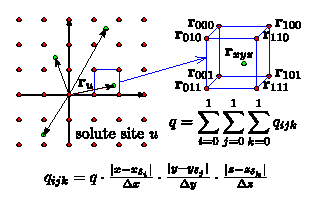
\includegraphics[scale=1.5]{_figure/charge_int_2}
\par\end{centering}
\caption{Solute charge density projected onto grids\label{fig:Charge-density-projected}}
\end{figure}

The electrostatic potential created by the charge distribution $\rho_{q}(\mathbf{r})$,
$V_{q}(\mathbf{r})$, can be thus computed using a periodic Poisson
Solver. The Poisson equation (\ref{eq:poisson})
\begin{equation}
\nabla^{2}V_{q}(\mathbf{r})=-\frac{\rho_{q}(\mathbf{r})}{\varepsilon_{0}}
\end{equation}
gives in Fourier space
\begin{equation}
\hat{V}_{q}(\mathbf{k})=\frac{\hat{\rho}_{q}(\mathbf{k})}{\varepsilon_{0}k^{2}}
\end{equation}
where $\hat{V}_{q}(\mathbf{k})$ and $\hat{\rho}_{q}(\mathbf{k})$
are the Fourier transform of $V_{q}(\mathbf{r})$ and $\rho_{q}(\mathbf{r})$
respectively. These two equations provide a fast way to calculate
$V_{q}(\mathbf{r})$ from $\rho_{q}(\mathbf{r})$.

The Coulomb potential is expressed as a sum of solvent partial charge
contributions at each grid node:
\begin{equation}
V_{\mathrm{coul}}(\mathbf{r},\mathbf{\Omega})=\sum_{v}q_{v}V_{q}(\mathbf{r}_{v})
\end{equation}
where $q_{v}$ is the point charge of solvent, and
\begin{equation}
\mathbf{r}_{v}=\mathbf{r}+\mathbf{R}(\mathbf{\Omega})\mathbf{s}_{v}
\end{equation}
is the cartesian coordinate of a solvent site $v$; $V_{q}(\mathbf{r}_{u})$
is the electrostatic potential, given by a linear interpolation of
the nearby point of $V_{q}(\mathbf{r})$ obtained in the last step
from the Poisson solver. 

Another method to calculate $V_{\mathrm{coul}}(\mathbf{r},\mathbf{\Omega})$
is the direct summation, which gives a non-periodic external potential,
but in the implementation it usually leads to better convergence for
non-spherical molecules. \marginpar{As in this thesis we only work on the $\mathcal{F}_{\mathrm{exc}}$
term.}Here we describe its expression, without understanding the reason
behind the convergence:
\begin{equation}
V_{\mathrm{coul}}(\mathbf{r},\mathbf{\Omega})=\sum_{u\in\mathrm{solute}}\sum_{v\in\mathrm{solvent}}\left(\dfrac{q_{u}q_{v}}{4\pi\varepsilon_{0}r_{uv}}\right)
\end{equation}
where $r_{uv}$ is calculated as in eq. (\ref{eq:4.ruv}). During
this thesis, the direct summation is only used in the minimization
of non-spherical solutes, in the chapters of implementation and application.

\subsection{The excess term\label{subsec:The-excess-term}}

As shown in $\mathsection$\ref{sec:Classical-density-functional},
we invoke here the \acs{HRF} approximation which amounts to a second-order
Taylor expansion around the homogeneous fluid at density $\rho_{0}$:
\begin{equation}
\mathcal{F}_{\mathrm{exc}}[\rho]=-\frac{k_{B}T}{2}\int\mathrm{d}\mathbf{r}_{1}\mathrm{d}\mathbf{\mathbf{\Omega}}\gamma(\mathbf{r}_{1},\mathbf{\mathbf{\mathbf{\mathbf{\Omega}}}})\rho(\mathbf{r}_{1},\mathbf{\mathbf{\mathbf{\mathbf{\Omega}}}})\label{eq:4.fexc}
\end{equation}
where $\gamma$ is the normalized gradient of the excess functional:
\begin{equation}
\gamma(\mathbf{r}_{1},\mathbf{\Omega}_{1})=-\frac{\delta\beta F_{\mathrm{exc}}}{\delta\rho}=\int\mathrm{d}\mathbf{r}_{2}\mathrm{d}\mathbf{\Omega}_{2}\Delta\rho(\mathbf{r}_{2},\mathbf{\Omega}_{2})c(\mathbf{r}_{12},\mathbf{\Omega}_{1},\mathbf{\Omega}_{2})\label{eq:4.gamma}
\end{equation}
which can be related to the solute-solvent 2-component \acs{IET}
with its definition:
\begin{equation}
\gamma_{\mathrm{MS}}(1,2)=h_{\mathrm{MS}}(1,2)-c_{\mathrm{MS}}(1,2)
\end{equation}

To evaluate the integration $\int\mathrm{d}\mathbf{r}_{2}\mathrm{d}\mathbf{\Omega}_{2}$
for each gradient $\gamma(\mathbf{r}_{1},\mathbf{\Omega}_{1})$ in
eq. (\ref{eq:4.gamma}), a total number of $N^{2}\equiv N_{\mathbf{r}}^{2}N_{\mathbf{\Omega}}^{2}=O(N^{2})$
function evaluations (\acs{FE}) are required, which, with typically
$N_{\mathbf{r}}=64^{3}$ and $N_{\mathbf{\Omega}}=50\sim100$, is
far too costly for current computing technology. For this reason,
Fourier transform is used to treat the spatial convolution.

A convolution
\begin{equation}
h(x_{1})\equiv f(x_{2})\otimes g(x_{2})\equiv\int_{a}^{b}f(x_{2})g(x_{1}-x_{2})dx_{2}\label{eq:convolution-1}
\end{equation}
has the property that
\begin{equation}
\mathfrak{F}[h(x_{1})]=\mathfrak{F}[f(x_{2})]\mathfrak{F}[g(x_{2})]\label{eq:convolution-2}
\end{equation}
$\mathfrak{F}$ being the Fourier transform operation. As $\mathbf{r}_{12}=\mathbf{r}_{1}-\mathbf{r}_{2}$,
eq. (\ref{eq:4.gamma}) is a 3D convolution, which leads to
\begin{equation}
\hat{\gamma}(\mathbf{k},\mathbf{\Omega}_{1})=\int\mathrm{d}\mathbf{\Omega}_{2}\Delta\hat{\rho}(\mathbf{k},\mathbf{\Omega}_{2})\hat{c}(\mathbf{k},\mathbf{\Omega}_{1},\mathbf{\Omega}_{2})\label{eq:4.gamma-k}
\end{equation}
Here we put the hat symbol on the physical quantities to represented
the Fourier transform of their original function.

In eq. (\ref{eq:4.gamma-k}), the integral $\int\mathrm{d}\mathbf{r}_{2}$
of eq. (\ref{eq:4.gamma}) is transformed into a simple product, only
$N_{\mathbf{r}}N_{\mathbf{\Omega}}^{2}$ \acs{FE} are needed to obtain
$\hat{\gamma}(\mathbf{k},\mathbf{\Omega}_{1})$ with given $\Delta\hat{\rho}(\mathbf{k},\mathbf{\Omega}_{2})$.
To this computational cost should be added the transform from $\Delta\rho(\mathbf{r},\mathbf{\Omega})$
to $\Delta\hat{\rho}(\mathbf{k},\mathbf{\Omega})$ and the backward
transform from $\hat{\gamma}(\mathbf{k},\mathbf{\Omega})$ to $\gamma(\mathbf{r},\mathbf{\Omega})$
which are both of order $N_{\mathbf{\Omega}}\cdot O(N_{\mathbf{r}}\log_{2}N_{\mathbf{r}})$
due to the properties of Fast Fourier Transforms (\acs{FFT}). The
total number of \acs{FE} is thus reduced from quadratic complexity
$O(N_{\mathbf{r}}^{2}N_{\mathbf{\Omega}}^{2})$ to $N_{\mathbf{r}}N_{\mathbf{\Omega}}^{2}+2N_{\mathbf{\Omega}}\cdot O(N_{\mathbf{r}}\log_{2}N_{\mathbf{r}})=O(N_{\mathbf{r}}\log_{2}N_{\mathbf{r}}N_{\mathbf{\Omega}}^{2})$.
As the total number of spatial grid $N_{\mathbf{r}}$ is of magnitude
$10^{5}\sim10^{6}$, this procedure, which is mathematically equivalent
to the direct evaluation (\ref{eq:4.gamma}), offers a great advantage
in terms of computational efficiency (figure \ref{fig:order-of-growth}
in appendix \ref{chpt:computing-performance}).

The angular-dependent \acs{DCF} of the homogeneous solvent, $\hat{c}(\mathbf{k},\mathbf{\Omega}_{1},\mathbf{\Omega}_{2})$,
is an input data which can be obtained from \acs{MD} or \acs{MC}
simulations. A detailed presentation of the \acs{DCF}s used in this
thesis is available in appendix \ref{chpt:dcf-water}.

\section{Molecular integral equation theory\label{sec:Angular-dependent-iem}}

To adapt the \acs{IET} formalism to non-spherical solvent, Blum \citep{Blum_I,Blum_II,blum_III}
proposed to expand the angle-dependent correlation functions $F(\mathbf{X}_{1},\mathbf{X}_{2})\equiv F(\mathbf{r}_{1},\mathbf{r}_{2},\mathbf{\Omega}_{1},\mathbf{\Omega}_{2})$
onto rotational invariants, such that the \acs{OZ} equation can be
reduced to only a few \acs{FE}. This theory is then adopted by Fries
\& Patey \citep{Fries_Patey_1985}, who proposed a numerical solution
for full \acs{HNC} closure. The test below describes the theory of
Blum, but based on the convention of Fries \& Patey, where Messiah's
definition of generalized spherical harmonics (\acs{GSH}s) is used.
A detailed explication of different conventions of \acs{GSH} is given
in appendix \ref{chpt:symmetry}.

\subsection{Translational and rotational invariance}

If $F$ describes a homogeneous fluid, the translational invariance
($\mathbf{r}_{12}\equiv\mathbf{r}_{1}-\mathbf{r}_{2}$) should be
presented, then the number of independent variables is reduced from
12 to 9:
\begin{equation}
F(\mathbf{X}_{1},\mathbf{X}_{2})=F(\mathbf{r}_{12},\mathbf{\Omega}_{1},\mathbf{\Omega}_{2})=F(r,\hat{\mathbf{r}}_{12},\mathbf{\Omega}_{1},\mathbf{\Omega}_{2})\label{eq:miet-def-func}
\end{equation}

We can further expand $F$ on Wigner \acs{GSH}s of the three orientations,
then $F$ becomes a sum of infinite number of projections that depending
on $r$ and 8 indices:
\begin{equation}
F(\mathbf{X}_{1},\mathbf{X}_{2})=\sum_{m,n,l=0}^{\infty}\sum_{\left|\mu',\mu\right|\leq m,\left|\nu',\nu\right|\leq n,\left|\lambda'\right|\leq l}F_{\mu'\mu\nu'\nu\lambda'}^{mnl}(r)R_{\mu'\mu}^{m}(\mathbf{\Omega}_{1})R_{\nu'\nu}^{m}(\mathbf{\Omega}_{2})R_{\lambda'0}^{l}(\hat{\mathbf{r}}_{12})
\end{equation}

Assuming that this expansion converges, which is normally the case
for correlation functions, the expansion can be expressed in limit
number of projections. If we also take into account the rotational
invariance by recombine some terms, only $r$ and 5 independent indices
are necessary to describe all the projections:
\begin{equation}
F_{\mu\nu}^{mnl}(r)=\sum_{\mu'\nu'\lambda'}\left(\begin{array}{ccc}
m & n & l\\
\mu' & \nu' & \lambda'
\end{array}\right)F_{\mu'\mu\nu'\nu\lambda'}^{mnl}(r)
\end{equation}

The projections $F_{\mu\nu}^{mnl}(r)$ with a finite order of expansion
have much fewer of terms compared to the angular form in eq. (\ref{eq:miet-def-func})
within the same precision of description.

We can define a basis set of rotational invariant as:
\begin{equation}
\Phi_{\mu\nu}^{mnl}(\mathbf{\Omega}_{1},\mathbf{\Omega}_{2},\mathbf{\hat{r}}_{12})=f^{mnl}\sum_{\mu'\nu'\lambda'}\left(\begin{array}{ccc}
m & n & l\\
\mu' & \nu' & \lambda'
\end{array}\right)R_{\mu'\mu}^{m}(\mathbf{\Omega}_{1})R_{\nu'\nu}^{n}(\mathbf{\Omega}_{2})R_{\lambda'0}^{l}(\mathbf{\hat{r}}_{12})
\end{equation}
where the normalization factor $f^{mnl}$ can be any arbitrary nonzero
constant, depending only on indices $m$, $n$, $l$. In Blum's convention,
it is taken as $\left[\left(2m+1\right)\left(2n+1\right)\right]^{\frac{1}{2}}$.

With these definitions, relation between the projections and the original
function is:
\begin{equation}
F(\mathbf{X}_{1},\mathbf{X}_{2})=\sum_{mnl\mu\nu}\tilde{F}_{\mu\nu}^{mnl}(r)\Phi_{\mu\nu}^{mnl}(\mathbf{\Omega}_{1},\mathbf{\Omega}_{2},\mathbf{\hat{r}}_{12})
\end{equation}
where $\tilde{F}_{\mu\nu}^{mnl}(r)=F_{\mu\nu}^{mnl}(r)/f^{mnl}$.

\subsection{Blum's reduction of molecular OZ equation}

The molecular Ornstein-Zernike (\acs{MOZ}) equation is defined as:
\begin{equation}
\gamma(\mathbf{X}_{1},\mathbf{X}_{2})=h(\mathbf{X}_{1},\mathbf{X}_{2})-c(\mathbf{X}_{1},\mathbf{X}_{2})=\frac{\rho}{8\pi^{2}}\int\mathrm{d}\mathbf{X}_{3}h(\mathbf{X}_{1},\mathbf{X}_{3})c(\mathbf{X}_{3},\mathbf{X}_{2})\label{eq:4.MOZ}
\end{equation}

The rotational invariant expansion gives:
\begin{equation}
c(\mathbf{X}_{1},\mathbf{X}_{2})=\sum_{mnl\mu\nu}c_{\mu\nu}^{mnl}(r)\Phi_{\mu\nu}^{mnl}(\mathbf{\Omega}_{1},\mathbf{\Omega}_{2},\mathbf{\hat{r}}_{12})
\end{equation}
\begin{equation}
\gamma(\mathbf{X}_{1},\mathbf{X}_{2})=\sum_{mnl\mu\nu}\gamma_{\mu\nu}^{mnl}(r)\Phi_{\mu\nu}^{mnl}(\mathbf{\Omega}_{1},\mathbf{\Omega}_{2},\mathbf{\hat{r}}_{12})
\end{equation}
and also in $k$-space:
\begin{equation}
\hat{c}(\mathbf{k},\mathbf{\Omega}_{1},\mathbf{\Omega}_{2})=\sum_{mnl\mu\nu}\hat{c}_{\mu\nu}^{mnl}(k)\Phi_{\mu\nu}^{mnl}(\mathbf{\Omega}_{1},\mathbf{\Omega}_{2},\mathbf{\hat{k}}_{12})
\end{equation}
\begin{equation}
\hat{\gamma}(\mathbf{k},\mathbf{\Omega}_{1},\mathbf{\Omega}_{2})=\sum_{mnl\mu\nu}\hat{\gamma}_{\mu\nu}^{mnl}(k)\Phi_{\mu\nu}^{mnl}(\mathbf{\Omega}_{1},\mathbf{\Omega}_{2},\mathbf{\hat{k}}_{12})
\end{equation}

The relation between these projections in $r$ and $k$-space are
built by the Hankel transform:
\begin{equation}
\hat{c}_{\mu\nu}^{mnl}(k)=4\pi i^{l}\int\mathrm{d}r\,r^{2}j_{l}(kr)c_{\mu\nu}^{mnl}(r)\label{eq:4.hankel1}
\end{equation}
\begin{equation}
\hat{\gamma}_{\mu\nu}^{mnl}(k)=4\pi i^{l}\int\mathrm{d}r\,r^{2}j_{l}(kr)\gamma_{\mu\nu}^{mnl}(r)\label{eq:4.hankel2}
\end{equation}
where $j_{l}(kr)$ are the spherical Bessel functions of order $l$.
Eq. (\ref{eq:4.hankel1}) and (\ref{eq:4.hankel2}) are built in the
same purpose as eq. (\ref{eq:3.oz-k}) in atomic case, where \acs{FFT}
is used. As an analogue to \acs{FFT}, the fast Hankel transform is
available for such a process. 

\textcolor{red}{Note that if function $f(\mathbf{X}_{1},\mathbf{X}_{2})$
is real and processes a symmetry axis $\mathrm{C}_{2v}$, like water,
the projections $f_{\mu\nu}^{mnl}(r)$ are real, therefore $\hat{f}_{\mu\nu}^{mnl}(k)$
is real if $l$ is even, and pure imaginary if $l$ is odd. The complete
symmetry relations are listed in $\mathsection$\ref{sec:Symmetry-rot_invar}.}

The \acs{MOZ} equation based on the rotational invariants $\hat{f}_{\mu\nu}^{mnl}(k)$
can be found in the article of Blum \citep{Blum_I}, but the form
is a bit complicate. To provide a simpler form, Blum defined the $\chi$-transform:
\begin{equation}
\hat{c'}_{\mu\nu,\chi}^{mn}(k)=\sum_{l=\left|m-n\right|}^{m+n}\left(\begin{array}{ccc}
m & n & l\\
\chi & -\chi & 0
\end{array}\right)\hat{c}_{\mu\nu}^{mnl}(k)
\end{equation}
\begin{equation}
\hat{\gamma'}_{\mu\nu,\chi}^{mn}(k)=\sum_{l=\left|m-n\right|}^{m+n}\left(\begin{array}{ccc}
m & n & l\\
\chi & -\chi & 0
\end{array}\right)\hat{\gamma}_{\mu\nu}^{mnl}(k)
\end{equation}
where we use the apostrophe to represent functions in an intermolecular
frame. 

The result \acs{MOZ} equation is:
\begin{equation}
\hat{\gamma'}_{\mu\nu,\chi}^{mn}(k)=\rho\sum_{n_{1}}\sum_{\nu_{1}=-n_{1}}^{n_{1}}(-)^{\chi+\nu_{1}}\left[\hat{\gamma'}_{\mu\nu_{1},\chi}^{mn_{1}}(k)+\hat{c'}_{\mu\nu_{1},\chi}^{mn_{1}}(k)\right]\hat{c'}_{\underline{\nu_{1}}\nu,\chi}^{n_{1}n}(k)
\end{equation}

This simple form of \acs{MOZ} equation reduces the calculation of
$\int\mathrm{d}\mathbf{X}_{3}$ for each $(\mathbf{X}_{1},\mathbf{X}_{2})$
in eq. (\ref{eq:4.MOZ}) to only a sum of terms of $n_{1}$, $\nu_{1}$
for each index of projection.



\chapter{Classical Density Functional Theory\label{chpt:mdft}}

Classical density functional theory provides a framework for determining
thermodynamic properties and correlation functions of a wide variety
of inhomogeneous (model) fluids starting from a microscopic basis,
i.e. the Hamiltonian describing interactions between particles. DFT
is based on the result that the grand potential of a specified inhomogeneous
fluid is a functional of the average one-body density,

\[
\rho(r)=\left\langle \sum_{i=1}^{N}\delta(\mathbf{r}-\mathbf{r}_{i})\right\rangle 
\]
where $\mathbf{r_{i}}$ is the position coordinate of particle $i$.

This article describes all the fundamental theories behind MDFT different
algorithms involved in this thesis to evaluate excess free energy
functional $\mathcal{F}_{\mathrm{exc}}$ under HRF approximation.


\section{Equilibrium Classical DFT}


\section{Variation principle}

The key idea is that $\mathcal{F}[\rho]$ is a unique functional of
$\rho(\mathbf{r})$; its form does not depend on the external potential
$V(\mathbf{r})$. \textcolor{red}{!!!!}

variation principe: par minimization

In \acf{MDFT}, the grand potential density functional corresponding
to an inhomogeneous fluid density $\rho(\mathbf{r},\mathbf{\Omega})$
is given by 
\begin{equation}
\Theta[\rho(\mathbf{r},\mathbf{\Omega})]=\Theta[\rho_{0}]+\mathcal{F}[\rho(\mathbf{r},\mathbf{\Omega})]
\end{equation}
Where $\Theta[\rho_{0}]$ is the correspondent reference bulk fluid
grand potential. And $\rho$ is the fluid density function variable
of 3 to 6 dimensions, including 3 coordinations for the position part,
and 0 to 3 for the angular part. For instance, in an isotropic fluid: 

\begin{equation}
\rho(\mathbf{r},\mathbf{\Omega})=\left\{ \begin{array}{ll}
n(\mathbf{r}) & \mbox{if atomic, }\Omega\equiv1\\
n(\mathbf{r})/4\pi & \mbox{if linear, }\Omega\equiv(\theta,\phi)\\
n(\mathbf{r})/8\pi^{2} & \mbox{if non-linear, }\Omega\equiv(\theta,\phi,\psi)
\end{array}\right.\label{eq:rho}
\end{equation}


Here the $4\pi$ and $8\pi^{2}$ is the normalization factor who equals
to $\int\mathrm{d}\mathbf{\Omega}$. The 6D definition of the latest
case in eq. \ref{eq:rho} of $\rho(\mathbf{r},\mathbf{\Omega})$ is
needed for arbitrary solvent, which results the most complex form
of the functional. 

According to the variation principle (c.f. Evans), the equilibrium
density can be found by minimizing the free energy functional $\mathcal{F}[\rho]$
regarding to $\rho(\mathbf{r},\mathbf{\Omega})$: 
\begin{equation}
\frac{\delta\mathcal{F}[\rho]}{\delta\rho(\mathbf{r},\mathbf{\Omega})}|_{\rho=\rho_{0}}=0
\end{equation}


And this functional is defined as a sum of functional contributions: 

\begin{equation}
\mathcal{F}[\rho]=\mathcal{F}_{\mathrm{id}}[\rho]+\mathcal{F}_{\mathrm{ext}}[\rho]+\mathcal{F}_{\mathrm{exc}}[\rho]
\end{equation}


The ideal term $\mathcal{F}_{\mathrm{id}}[\rho]$ is deduced from
the particle interaction-free condition: 
\begin{equation}
\mathcal{F}_{\mathrm{id}}[\rho]=\beta^{-1}\int\mathrm{d}\mathbf{r}\mathrm{d\Omega}\left[\mathbf{\mathbf{\ln\left(\frac{\rho(\mathbf{r},\mathbf{\mathbf{\mathbf{\mathbf{\Omega}}}})}{\rho_{0}}\right)}}-\rho(\mathbf{r},\mathbf{\mathbf{\mathbf{\Omega}}})+\rho_{0}\right]
\end{equation}
Where $\beta=\left(K_{\mathrm{B}}T\right)^{-1}$ and $\rho_{0}$ is
the reference bulk density of pure solvent. 

The external potential term calculates the contribution of solute
external potential $V_{\mathrm{ext}}$: 
\begin{equation}
\mathcal{F}_{\mathrm{ext}}[\rho]=\int\mathrm{d}\mathbf{r}\mathrm{d}\mathbf{\mathbf{\Omega}}V_{\mathrm{ext}}(\mathbf{r},\mathbf{\mathbf{\mathbf{\mathbf{\Omega}}}})\rho(\mathbf{r},\mathbf{\mathbf{\mathbf{\mathbf{\Omega}}}})
\end{equation}


\begin{equation}
V_{\mathrm{ext}}(\mathbf{r},\mathbf{\mathbf{\mathbf{\mathbf{\Omega}}}})=\sum_{j\in\mathrm{solvent}}\left\{ q_{j}V_{q}(\mathbf{r}_{j})+\sum_{i\in\mathrm{solute}}4\epsilon_{ij}\left[\left(\frac{\sigma_{ij}}{r_{ij}}\right)^{12}-\left(\frac{\sigma_{ij}}{r_{ij}}\right)^{6}\right]\right\} 
\end{equation}
Where $V_{\mathrm{ext}}$ is pre-calculated and stored as a 6-dimension
double precision (8 bytes per real value) table. It contains the contribution
of Lennard-Jones interaction and electrostatic potential. 

This two terms $\mathcal{F}_{\mathrm{id}}[\rho]$ and $\mathcal{F}_{\mathrm{ext}}[\rho]$
are physically exact. 

The excess term $\mathcal{F}_{\mathrm{exc}}[\rho]$ depend on the
exact correlation function, which is a priori unknown: 
\begin{equation}
C(\mathbf{r}_{1},\mathbf{r}_{2},\mathbf{\Omega}_{1},\mathbf{\Omega}_{2};\rho)\equiv\frac{\beta\delta^{2}\mathcal{F}_{\mathrm{exc}}[\rho]}{\delta\rho(\mathbf{r}_{1},\mathbf{\Omega}_{1})\delta\rho(\mathbf{r}_{2},\mathbf{\Omega}_{2})}
\end{equation}


The ideal term $\mathcal{F}_{id}[\rho]$ is deduced from the condition
that the interaction potential of particles $\Phi=0$ 
\[
Z_{N}(\beta,V)=\frac{\lambda^{-3N}}{N!}\int_{V}d\mathbf{r}^{N}e^{-\beta\Phi}=\frac{\lambda^{-3N}}{N!}V^{N}
\]
\[
F_{N}(\beta,V)=-\beta^{-1}\log{Z_{N}}=\beta^{-1}\log{(N!\lambda^{3N}V^{-N})}=\beta^{-1}(N\log{\lambda^{3}\rho}-N)
\]


(also available for the in homogenous case.) Since we define 
\[
\mathcal{F}_{id}[\rho]=\int d\mathbf{X}f_{id}[\rho(\mathbf{X})]
\]
We have 
\[
f_{id}[\rho(\mathbf{X})]=\beta^{-1}\Delta\rho(\log{\lambda^{3}\Delta\rho}-1)
\]
and 
\[
\mathcal{F}_{id}[\rho]=\beta^{-1}\int d\mathbf{X}_{1}[\rho(\mathbf{X}_{1})\log{(\frac{\rho(\mathbf{X}_{1})}{\rho_{0}})}-\rho(\mathbf{X}_{1})+\rho_{0}]
\]


The external potential term 
\[
\mathcal{F}_{ext}[\rho]=\int d\mathbf{X}_{1}V_{ext}(\mathbf{X}_{1})\rho(\mathbf{X}_{1})
\]
Where $V_{ext}$ is given by table.

The exact (in an approximation that C do not depend on $\rho$) form
of the excess term $\mathcal{F}_{exc}$ is 
\[
\mathcal{F}_{exc}[\rho]=\beta^{-1}\int d\mathbf{X}_{1}d\mathbf{X}_{2}\Delta\rho(\mathbf{X}_{1})\Delta\rho(\mathbf{X}_{2})C(\mathbf{X}_{1},\mathbf{X}_{2};\rho)
\]


where $C(\mathbf{X}_{1},\mathbf{X}_{2};\rho)$ is the correlation
function, a priori unknown, which definition is: 
\[
C(\mathbf{X}_{1},\mathbf{X}_{2};\rho)=\frac{\beta\delta^{2}\mathcal{F}_{exc}[\rho]}{\delta\rho(\mathbf{r}_{1})\delta\rho(\mathbf{r}_{2})}
\]


structure MDFT

The code MDFT is built for minimizing the free energy functional $\mathcal{F}[\rho]$
by minimizer L-BFGS (ref). It's main structure is shown in fig. 

\begin{figure}[h]
\caption{\selectlanguage{english}%
Flowchart of code MDFT\selectlanguage{american}%
}
\end{figure}


The minimizer requires the functional and its gradient as input, and
produce at each iteration a new fluid density $\text{\ensuremath{\rho}(\ensuremath{\mathbf{r}},\ensuremath{\mathbf{\mathbf{\mathbf{\Omega}}}})}$
nearer to the equilibrium density. The objective for \textbf{branch
hesper} is to calculate the excess term $\mathcal{F}_{\mathrm{exc}}[\rho]$
of the functional in eq.\ref{eq:F_exc}, as well as its gradient: 

\begin{equation}
\gamma(\mathbf{r}_{1},\mathbf{\Omega})=\frac{\delta\mathcal{F}_{\mathrm{exc}}}{\delta\rho}=-\beta^{-1}\int d\mathbf{r}_{2}d\mathbf{\Omega}_{2}\Delta\rho(\mathbf{r}_{2},\mathbf{\Omega}_{2})c^{(2)}(\mathbf{r}_{12},\mathbf{\Omega}_{1},\mathbf{\Omega}_{2})\label{eq:gradient}
\end{equation}



\section{Ideal free energy}


\section{External free energy}


\subsection{Electrostatic potential}

The direct evaluation of the Coulomb sum for $N$ particles is 
\begin{equation}
U_{C}=\sum_{i<j}a\frac{q_{i}q_{j}}{\left\Vert \bm{r}_{i}-\bm{r}_{j}\right\Vert },\label{eq:direct-coulomb-sum}
\end{equation}
where $a$ is a constant that gives $U_{C}$ the dimension of an energy,
and $q_{i}$,$\bm{r}_{i}$ are the charge and position of particle
$i$. The computation of equation \ref{eq:direct-coulomb-sum} is
demanding because it requires a large number of distances $r_{ij}\equiv\left\Vert \bm{r}_{i}-\bm{r}_{j}\right\Vert $
to be computed. In our case, we have $\textrm{nfft}_{1}\times\textrm{nfft}_{2}\times\textrm{nfft}_{3}\times N_{\bm{\Omega}}\times N_{\psi}\times N_{q_{v}}$,
where $N_{q_{v}}$ is the number of point charges of the solvent molecule,
to be computed per point charge of the solute. This is typically $10^{9}$
distances for MDFT.

L'énergie électrostatique s'écrit
\begin{eqnarray}
\mathcal{F}_{q} & = & \frac{1}{2}\iiint\frac{\rho_{c}^{\textrm{soluté}}\left(\boldsymbol{r^{\prime}}\right)\rho_{c}^{\textrm{solvant}}\left(\boldsymbol{r},\boldsymbol{\Omega}\right)}{4\pi\epsilon_{0}\left\Vert \boldsymbol{r}-\boldsymbol{r^{\prime}}\right\Vert }\textrm{d}\boldsymbol{r}\textrm{d}\boldsymbol{r^{\prime}}\textrm{d}\boldsymbol{\Omega}\\
 & = & \frac{1}{2}\frac{1}{4\pi\epsilon_{0}}\iiint\frac{\rho_{c}^{\textrm{soluté}}\left(\boldsymbol{r^{\prime}}\right)}{\left\Vert \boldsymbol{r}-\boldsymbol{r^{\prime}}\right\Vert }\left[\rho^{\textrm{solvant}}*\sigma\right]\left(\boldsymbol{r},\boldsymbol{\Omega}\right)\textrm{d}\boldsymbol{r}\textrm{d}\boldsymbol{r^{\prime}}\textrm{d}\boldsymbol{\Omega}\\
 & = & \frac{1}{2}\frac{1}{4\pi\epsilon_{0}}\iint\left[\rho_{c}^{\textrm{soluté}}*\left\Vert \boldsymbol{r}\right\Vert ^{-1}\right]\left(\boldsymbol{r},\boldsymbol{\Omega}\right)\left[\rho^{\textrm{solvant}}*\sigma\right]\left(\boldsymbol{r},\boldsymbol{\Omega}\right)\textrm{d}\boldsymbol{r}\textrm{d}\boldsymbol{\Omega}\\
 & =
\end{eqnarray}


On définit une densité de charge d'une molécule $\boldsymbol{\sigma}\left(\boldsymbol{r},\boldsymbol{\Omega}\right)$:
\begin{equation}
\boldsymbol{\sigma}\left(\boldsymbol{r},\boldsymbol{\Omega}\right)=\sum_{m=1}^{\textrm{sites du solvant}}q_{m}\delta\left(\boldsymbol{r}-\boldsymbol{s}_{m}\left(\boldsymbol{\Omega}\right)\right).
\end{equation}
$\boldsymbol{s}_{m}\left(\boldsymbol{\Omega}\right)$ désigne la position
du $m^{\textrm{ième}}$ site de la molécule de solvant quand elle
a l'orientation $\boldsymbol{\Omega}$.


\section{Excess free energy}

In the molecular density functional theory (MDFT), the excess free
energy functional $\mathcal{F}_{\mathrm{exc}}$ can be developed via
Taylor expansion 
\begin{equation}
\mathcal{F}_{\mathrm{exc}}\left[\rho\right]\equiv\mathcal{F}_{\mathrm{exc}}\left[\rho_{0}\right]+\int\mathrm{d}\mathbf{X_{1}}\frac{\delta\mathcal{F}_{\mathrm{exc}}\left[\rho\right]}{\mathrm{\delta}\rho(\mathbf{X_{1}})}\Delta\rho(\mathbf{X_{1}})+\frac{1}{2}\int\mathrm{d}\mathbf{X_{1}}\mathrm{d}\mathbf{X_{2}}\frac{\mathrm{\delta}^{2}\mathcal{F}_{\mathrm{exc}}\left[\rho\right]}{\mathrm{\delta}\rho(\mathbf{X_{1}})\mathrm{\delta}\rho(\mathbf{X_{2}})}\Delta\rho(\mathbf{X_{1}})\Delta\rho(\mathbf{X_{2}})+\mathcal{O}(\Delta\rho^{3})\label{eq:Taylor-1}
\end{equation}
where $\mathbf{X}\equiv(\mathbf{r},\mathbf{\Omega})$, $\beta^{-1}=k_{\mathrm{B}}T$,
$\Delta\rho=\rho-\rho_{0}$, and $\rho(\mathbf{X})$ the single-particle
density of the fluid.


\subsection{Homogenous Reference Fluid Approximation}

According to the variation principle, the first derivative in eq.
(\ref{eq:Taylor-1}) is zero
\begin{equation}
\left.\frac{\mathrm{\delta}\mathcal{F}_{\mathrm{exc}}\left[\rho\right]}{\mathrm{\delta}\rho(\mathbf{X_{1}})}\right|_{\rho=\rho_{\mathrm{eq}}}=0
\end{equation}


And $\mathcal{F}_{\mathrm{exc}}\left[\rho_{0}\right]$ can be compensated
by the grand potential of bulk fluid (to be detailed), we can then
focus on only $\mathcal{O}(\Delta\rho^{2})$ and higher order terms.

As $\mathcal{F}_{\mathrm{exc}}$ is a generating functional of $c^{(n)}(\mathbf{X}^{n})$,
the direct correlations functions (DCF) \citep{Hensen-McDonald},
for example
\begin{equation}
c^{(2)}(\mathbf{X_{1}},\mathbf{X_{2}})=-\beta\frac{\mathrm{\delta}^{2}\mathcal{F}_{\mathrm{exc}}\left[\rho\right]}{\mathrm{\delta}\rho(\mathbf{X_{1}})\mathrm{\delta}\rho(\mathbf{X_{2}})}
\end{equation}
eq. (\ref{eq:Taylor-1}) can be rewritten as
\begin{eqnarray}
\mathcal{F}_{\mathrm{exc}}\left[\rho\right] & = & -\frac{\beta^{-1}}{2}\int\mathrm{d}\mathbf{X_{1}}\mathrm{d}\mathbf{X_{2}}c^{(2)}(\mathbf{X_{1}},\mathbf{X_{2}})\Delta\rho(\mathbf{X_{1}})\Delta\rho(\mathbf{X_{2}})+\mathcal{O}(\Delta\rho^{3})\nonumber \\
 & \simeq & -\frac{\beta^{-1}}{2}\int\mathrm{d}\mathbf{X_{1}}\mathrm{d}\mathbf{X_{2}}c^{(2)}(\mathbf{X_{1}},\mathbf{X_{2}})\Delta\rho(\mathbf{X_{1}})\Delta\rho(\mathbf{X_{2}})\label{eq:fexc-2nd-term-1}
\end{eqnarray}


If we take further approximation, to assume that
\begin{equation}
c^{(2)}(\mathbf{X_{1}},\mathbf{X_{2}})\simeq c_{0}^{(2)}(\mathbf{X_{1}},\mathbf{X_{2}})
\end{equation}
where $c_{0}^{(2)}(\mathbf{X_{1}},\mathbf{X_{2}})$ is the DCF of
the bulk fluid, it's called the homogenous reference fluid (HRF) approximation.


\subsection{nn\_cs}

We define $r=\left\Vert \bm{r}-\bm{r}^{\prime}\right\Vert $, and
$\Delta n\left(\bm{r}\right)=n\left(\bm{r}\right)-n_{0}$, and $n_{0}$
the density (given in dft.in) of the homogeneous fluid of reference,
e.g., 0.0332891 molecule per \AA$^3$ for water.

We also define $n\left(\bm{r}\right)=\int\rho(\bm{r},\boldsymbol{\Omega})\mbox{d}\boldsymbol{\Omega}$.
We have 
\begin{eqnarray}
F_{exc} & = & -\frac{1}{2}k_{B}T\iint\Delta n\left(\boldsymbol{r}\right)\Delta n\left(\boldsymbol{r}^{\prime}\right)c\left(r\right)d\bm{r}d\bm{r}^{\prime},
\end{eqnarray}


Now, we consider the convolution in the right hand side of the equation,
$\gamma\equiv\left(\Delta n*c\right)$, that can be computed much
efficiently than in $O\left(N^{2}\right)$ by fast Fourier transform
in $O\left(N\log N\right)$.

\uline{Inputs:}
\begin{itemize}
\item $\rho\left(\bm{r},\Omega\right)$
\item $c_{s}\left(k\right)$, with $k\equiv\left\Vert \bm{k}\right\Vert $
\item functions to Fast Fourier Transform (FFT) and inverse Fast Fourier
Transform (FFT$^{-1}$)
\item $n_{0}$, the density of the homogeneous fluid of reference
\item $T$ the temperature in Kelvin
\item $k_{B}$ the Boltzmann constant.
\end{itemize}

\subsection{polarisation}

\begin{equation}
\mathcal{F}_{exc}=-\frac{k_{B}T}{2}\iiint_{\mathcal{R}^{3}}\int_{\theta=0}^{\pi}\int_{\phi=0}^{2\pi}\int_{\psi=0}^{2\pi}\Delta\rho\left(\bm{r}_{1},\bm{\Omega}_{1}\right)c^{\left(2\right)}\left(\bm{r}_{1},\bm{r}_{2},\bm{\Omega}_{1},\bm{\Omega}_{2}\right)\Delta\rho\left(\bm{r}_{2},\bm{\Omega}_{2}\right)d\bm{r}_{1}d\bm{r}_{2}d\bm{\Omega}_{1}d\bm{\Omega}_{2}
\end{equation}
where $\rho=n/\left(8\pi^{2}\right)$ and we define 
\begin{eqnarray}
\bm{P}\left(\bm{r}\right) & = & \int\bm{p}\rho\left(\bm{r},\bm{\Omega}\right)d\bm{\Omega}
\end{eqnarray}
with $\bm{p}=p\bm{\Omega}$ the dipolar moment of a water molecule.


\section{OZ Equation in MDFT and IEM Formalism}

Ornstein-Zernike (OZ) equation is a fundamental equation to the theory
of liquids, which defined $c^{(2)}(\mathbf{X_{1}},\mathbf{X_{2}})$.
Its most common form is as shown \citep{Hensen-McDonald}:

\begin{equation}
h^{(2)}(\mathbf{X_{1}},\mathbf{X_{2}})=c^{(2)}(\mathbf{X_{1}},\mathbf{X_{2}})+\int c^{(2)}(\mathbf{X_{1}},\mathbf{X_{3}})\rho(\mathbf{X_{3}})h^{(2)}(\mathbf{X_{3}},\mathbf{X_{2}})\mathrm{d}\mathbf{X_{3}}\label{eq:oz-iem-2}
\end{equation}
where $h^{(2)}(\mathbf{X_{1}},\mathbf{X_{2}})$ is the pair correlation
function (PCF). When the fluid is homogenous, eq. (\ref{eq:oz-iem-2})
becomes:

\begin{equation}
h^{(2)}(\mathbf{X_{1}},\mathbf{X_{2}})=c^{(2)}(\mathbf{X_{1}},\mathbf{X_{2}})+\rho_{0}\int c^{(2)}(\mathbf{X_{1}},\mathbf{X_{3}})h^{(2)}(\mathbf{X_{3}},\mathbf{X_{2}})\mathrm{d}\mathbf{X_{3}}\label{eq:oz-iem-1-1}
\end{equation}
which gives 
\begin{equation}
\gamma(\mathbf{X_{1}},\mathbf{X_{2}})=h^{(2)}(\mathbf{X_{1}},\mathbf{X_{2}})-c^{(2)}(\mathbf{X_{1}},\mathbf{X_{2}})=\rho_{0}\int c^{(2)}(\mathbf{X_{1}},\mathbf{X_{3}})h^{(2)}(\mathbf{X_{3}},\mathbf{X_{2}})\mathrm{d}\mathbf{X_{3}}\label{eq:gamma-oz-2}
\end{equation}


If we take $\mathbf{X_{2}}$ as origin in the laboratory coordinate
system, eq. (\ref{eq:gamma-oz-2}) becomes:
\begin{equation}
\gamma(\mathbf{X_{1}})=\int c^{(2)}(\mathbf{X}_{1},\mathbf{X_{3}})\Delta\rho(\mathbf{X_{3}})\mathrm{d}\mathbf{X_{3}}\label{eq:gamma-oz-1-1}
\end{equation}
which coincides with the gradient of $\mathcal{F}_{\mathrm{exc}}\left[\rho\right]$
in eq. (\ref{eq:fexc-2nd-term-1}).

It can be further proved that the homogenous reference fluid (HRF)
approximation of molecular density functional theory (MDFT) is mathematically
equivalent to the hypernetted chain (HNC) approximation to integral
equations method (IEM) if the fluid is homogenous. (To be detailed.)


\section{Statistical mechanics}


\section{Principe of Variation}


\section{Ideal free energy functional}


\section{External free energy functional}


\section{Homogenous Reference Fluid Approximation}

In the molecular density functional theory (MDFT), the excess free
energy functional $\mathcal{F}_{\mathrm{exc}}$ can be developed via
Taylor expansion 
\begin{equation}
\mathcal{F}_{\mathrm{exc}}\left[\rho\right]\equiv\mathcal{F}_{\mathrm{exc}}\left[\rho_{0}\right]+\int\mathrm{d}\mathbf{X_{1}}\frac{\delta\mathcal{F}_{\mathrm{exc}}\left[\rho\right]}{\mathrm{\delta}\rho(\mathbf{X_{1}})}\Delta\rho(\mathbf{X_{1}})+\frac{1}{2}\int\mathrm{d}\mathbf{X_{1}}\mathrm{d}\mathbf{X_{2}}\frac{\mathrm{\delta}^{2}\mathcal{F}_{\mathrm{exc}}\left[\rho\right]}{\mathrm{\delta}\rho(\mathbf{X_{1}})\mathrm{\delta}\rho(\mathbf{X_{2}})}\Delta\rho(\mathbf{X_{1}})\Delta\rho(\mathbf{X_{2}})+\mathcal{O}(\Delta\rho^{3})\label{eq:Taylor}
\end{equation}
where $\mathbf{X}\equiv(\mathbf{r},\mathbf{\Omega})$, $\beta^{-1}=k_{\mathrm{B}}T$,
$\Delta\rho=\rho-\rho_{0}$, and $\rho(\mathbf{X})$ the single-particle
density of the fluid.

According to the variation principle, the first derivative in eq.
(\ref{eq:Taylor}) is zero
\begin{equation}
\left.\frac{\mathrm{\delta}\mathcal{F}_{\mathrm{exc}}\left[\rho\right]}{\mathrm{\delta}\rho(\mathbf{X_{1}})}\right|_{\rho=\rho_{\mathrm{eq}}}=0
\end{equation}


And $\mathcal{F}_{\mathrm{exc}}\left[\rho_{0}\right]$ can be compensated
by the grand potential of bulk fluid (to be detailed), we can then
focus on only $\mathcal{O}(\Delta\rho^{2})$ and higher order terms.

As $\mathcal{F}_{\mathrm{exc}}$ is a generating functional of $c^{(n)}(\mathbf{X}^{n})$,
the direct correlations functions (DCF) \citep{Hensen-McDonald},
for example
\begin{equation}
c^{(2)}(\mathbf{X_{1}},\mathbf{X_{2}})=-\beta\frac{\mathrm{\delta}^{2}\mathcal{F}_{\mathrm{exc}}\left[\rho\right]}{\mathrm{\delta}\rho(\mathbf{X_{1}})\mathrm{\delta}\rho(\mathbf{X_{2}})}
\end{equation}
eq. (\ref{eq:Taylor}) can be rewritten as
\begin{eqnarray}
\mathcal{F}_{\mathrm{exc}}\left[\rho\right] & = & -\frac{\beta^{-1}}{2}\int\mathrm{d}\mathbf{X_{1}}\mathrm{d}\mathbf{X_{2}}c^{(2)}(\mathbf{X_{1}},\mathbf{X_{2}})\Delta\rho(\mathbf{X_{1}})\Delta\rho(\mathbf{X_{2}})+\mathcal{O}(\Delta\rho^{3})\nonumber \\
 & \simeq & -\frac{\beta^{-1}}{2}\int\mathrm{d}\mathbf{X_{1}}\mathrm{d}\mathbf{X_{2}}c^{(2)}(\mathbf{X_{1}},\mathbf{X_{2}})\Delta\rho(\mathbf{X_{1}})\Delta\rho(\mathbf{X_{2}})\label{eq:fexc-2nd-term}
\end{eqnarray}


If we take further approximation, to assume that
\begin{equation}
c^{(2)}(\mathbf{X_{1}},\mathbf{X_{2}})\simeq c_{0}^{(2)}(\mathbf{X_{1}},\mathbf{X_{2}})
\end{equation}
where $c_{0}^{(2)}(\mathbf{X_{1}},\mathbf{X_{2}})$ is the DCF of
the bulk fluid, it's called the homogenous reference fluid (HRF) approximation.


\section{OZ Equation in MDFT and IEM Formalism}

Ornstein-Zernike (OZ) equation is a fundamental equation to the theory
of liquids, which defined $c^{(2)}(\mathbf{X_{1}},\mathbf{X_{2}})$.
Its most common form is as shown \citep{Hensen-McDonald}:

\begin{equation}
h^{(2)}(\mathbf{X_{1}},\mathbf{X_{2}})=c^{(2)}(\mathbf{X_{1}},\mathbf{X_{2}})+\int c^{(2)}(\mathbf{X_{1}},\mathbf{X_{3}})\rho(\mathbf{X_{3}})h^{(2)}(\mathbf{X_{3}},\mathbf{X_{2}})\mathrm{d}\mathbf{X_{3}}\label{eq:oz-iem}
\end{equation}
where $h^{(2)}(\mathbf{X_{1}},\mathbf{X_{2}})$ is the pair correlation
function (PCF). When the fluid is homogenous, eq. (\ref{eq:oz-iem})
becomes:

\begin{equation}
h^{(2)}(\mathbf{X_{1}},\mathbf{X_{2}})=c^{(2)}(\mathbf{X_{1}},\mathbf{X_{2}})+\rho_{0}\int c^{(2)}(\mathbf{X_{1}},\mathbf{X_{3}})h^{(2)}(\mathbf{X_{3}},\mathbf{X_{2}})\mathrm{d}\mathbf{X_{3}}\label{eq:oz-iem-1}
\end{equation}
which gives 
\begin{equation}
\gamma(\mathbf{X_{1}},\mathbf{X_{2}})=h^{(2)}(\mathbf{X_{1}},\mathbf{X_{2}})-c^{(2)}(\mathbf{X_{1}},\mathbf{X_{2}})=\rho_{0}\int c^{(2)}(\mathbf{X_{1}},\mathbf{X_{3}})h^{(2)}(\mathbf{X_{3}},\mathbf{X_{2}})\mathrm{d}\mathbf{X_{3}}\label{eq:gamma-oz}
\end{equation}


If we take $\mathbf{X_{2}}$ as origin in the laboratory coordinate
system, eq. (\ref{eq:gamma-oz}) becomes:
\begin{equation}
\gamma(\mathbf{X_{1}})=\int c^{(2)}(\mathbf{X}_{1},\mathbf{X_{3}})\Delta\rho(\mathbf{X_{3}})\mathrm{d}\mathbf{X_{3}}\label{eq:gamma-oz-1}
\end{equation}
which coincides with the gradient of $\mathcal{F}_{\mathrm{exc}}\left[\rho\right]$
in eq. (\ref{eq:fexc-2nd-term}).

It can be further proved that the homogenous reference fluid (HRF)
approximation of molecular density functional theory (MDFT) is mathematically
equivalent to the hypernetted chain (HNC) approximation to integral
equations method (IEM) if the fluid is homogenous. (To be detailed.)


\section{Supercell discretization}

$L_{x}\times L_{y}\times L_{z}$ Å$^{3}$ space is discretized on
a regular grid of $\textrm{nfft}_{1}\times\textrm{nfft}_{2}\times\textrm{nfft}_{3}$
nodes. Angular grid is discretized with Lebedev (L) or Gauss-Legendre
(GL) quadrature for $\bm{\Omega}\equiv\left\{ \theta,\phi\right\} ,\theta\in\left[0,\pi\right],\phi\in\left[0,2\pi\right]$,
and regular quadrature for $\psi\in\left[0,\pi\right]$.


\paragraph{translate\_solute\_to\_center = \{\uline{T},F\}\protect \\
}

This translates your solute to the center of the supercell: all solute
coordinates are moved by \{Lx/2., Ly/2., Lz/2.\}, with \{Lx,Ly,Lz\}
the length of the supercell.


\section{cg\_vect}


\subsection{Multipolar polarization}

We define a charge density $\sigma\left(\bm{r},\bm{\Omega}\right)$
and polarization density $\bm{p}\left(\bm{r},\bm{\Omega}\right)$
of a molecule at the origin of the cartesian reference frame with
orientation $\bm{\Omega}$.
\begin{equation}
\sigma\left(\bm{r},\bm{\Omega}\right)=\sum_{m}q_{m}\delta\left(\bm{r}-\bm{s}_{m}\left(\bm{\Omega}\right)\right)
\end{equation}
in the general case, and 
\begin{equation}
\sigma\left(\bm{r},\bm{\Omega}\right)=q_{O}\delta\left(\bm{r}\right)+q_{H}\delta\left(\bm{r}-\bm{s}_{H_{1}}\left(\bm{\Omega}\right)\right)+q_{H}\delta\left(\bm{r}-\bm{s}_{H_{2}}\left(\bm{\Omega}\right)\right)
\end{equation}
for a single SPC-type water molecule with oxygen at the origin.


\section{Poisson solver : Iterative solvers for linear equations}

Given a square system of $n$ linear equations:

\begin{equation}
\bm{A}\bm{x}=\bm{b}.\label{eq:linsys}
\end{equation}
 Some (very slow) direct techniques exist that involve algebra. We
will solve this equation by an iterative (also called relaxation)
method. We will use a sequence of $\bm{x}^{\left(k\right)}$ that
converges toward the fixed point $\bm{x}$, solution of our problem.

In conclusion, we want to write, for a given $\bm{x}^{\left(0\right)}$,
a sequence $\bm{x}^{\left(k+1\right)}=F\left(\bm{x}^{\left(k\right)}\right)$
with $k\in\mathbb{N}$.


\section{Jacobi's method}

We decompose $A=D-L-U$ where $D$ is an inversible matrix.
\begin{equation}
\bm{A}\bm{x}=\bm{b}\Leftrightarrow\bm{D}\bm{x}=\left(\bm{L}+\bm{U}\right)\bm{x}+\bm{b}
\end{equation}
\begin{eqnarray}
\Leftrightarrow\bm{x} & = & \bm{D}^{-1}\left(\bm{L}+\bm{U}\right)\bm{x}+\bm{D}^{-1}\bm{b}\\
 & = & F\left(\bm{x}\right)
\end{eqnarray}
where $F$ is a linear function of $x$.

It is shown that we can solve this equation by iteratively solving,
where $k$ indicates the iteration number
\begin{equation}
\bm{x}^{\left(k+1\right)}=\bm{D}^{-1}\left(\bm{L}+\bm{U}\right)\bm{x}^{\left(k\right)}+\bm{D}^{-1}\bm{b}.
\end{equation}
Since $\mbox{diag}\left(\left(\bm{L}+\bm{U}\right)\bm{x}^{\left(k\right)}\right)=\bm{0}$,
each $x_{i}^{\left(k+1\right)}$ is independent of $x_{i}^{\left(k\right)}$.
It is instead a weighted average of other $x_{j\neq i}$. Since we
don't know the solution \emph{a priori}, we define the residual at
each step $k$ as $\bm{r}^{\left(k\right)}=\bm{b}-\bm{A}\bm{x}^{\left(k\right)}$.
See algorithm~\ref{alg:Jacobi's-algorithm}.

\begin{algorithm}[h]
\uline{Output}
\begin{itemize}
\item $\bm{x}$, an approximate solution to $\bm{A}\bm{x}=\bm{b}$ where
$\bm{A}$ and $\bm{b}$ are known.
\end{itemize}
\uline{Inputs}
\begin{itemize}
\item $\bm{A}$
\item $\bm{b}$
\item $\bm{x}^{\left(0\right)}$ including boundary conditions. No restriction
on $\bm{x}^{\left(0\right)}$.
\item $\epsilon$, the tolerance or convergence criteria. A suitable tolerance
might be $\left\Vert \bm{r}^{\left(k\right)}\right\Vert <\epsilon$
or $\left\Vert \bm{r}^{\left(k\right)}-\bm{r}^{\left(k-1\right)}\right\Vert <\epsilon$. 
\end{itemize}
\uline{Restrictions}
\begin{itemize}
\item $\bm{A}$ must be strictly diagonaly dominant, \emph{i.e.}, $\left|A_{i,i}\right|>\sum_{j=1,n;j\neq i}\left|A_{i,j}\right|$
$\Rightarrow A_{i,i}\neq0$.
\item $\epsilon>0$
\end{itemize}
\uline{Algo}
\begin{enumerate}
\item $\bm{D}\longleftarrow\mbox{diag}\left(\bm{A}\right)$
\item $\bm{R}\longleftarrow\bm{D}-\bm{A}$
\item $\bm{D}^{-1}\longleftarrow1/\bm{D}$
\item do while $\xi\geq\epsilon$ 

\begin{enumerate}
\item $\bm{x}_{\mathrm{old}}\longleftarrow\bm{x}$
\item $\bm{x}\longleftarrow\bm{D}^{-1}\bm{R}\bm{x}_{\mathrm{old}}+\bm{D}^{-1}\bm{b}$
\item $\bm{r}\longleftarrow\bm{A}\bm{x}-\bm{b}$
\item $\xi\longleftarrow\left\Vert \bm{r}\right\Vert $
\end{enumerate}
\end{enumerate}
\caption{\selectlanguage{english}%
Jacobi's algorithm\label{alg:Jacobi's-algorithm}\selectlanguage{american}%
}
\end{algorithm}



\section{vext q}

L'énergie électrostatique s'écrit
\begin{eqnarray}
\mathcal{F}_{q} & = & \frac{1}{2}\iiint\frac{\rho_{c}^{\textrm{soluté}}\left(\boldsymbol{r^{\prime}}\right)\rho_{c}^{\textrm{solvant}}\left(\boldsymbol{r},\boldsymbol{\Omega}\right)}{4\pi\epsilon_{0}\left\Vert \boldsymbol{r}-\boldsymbol{r^{\prime}}\right\Vert }\textrm{d}\boldsymbol{r}\textrm{d}\boldsymbol{r^{\prime}}\textrm{d}\boldsymbol{\Omega}\\
 & = & \frac{1}{2}\frac{1}{4\pi\epsilon_{0}}\iiint\frac{\rho_{c}^{\textrm{soluté}}\left(\boldsymbol{r^{\prime}}\right)}{\left\Vert \boldsymbol{r}-\boldsymbol{r^{\prime}}\right\Vert }\left[\rho^{\textrm{solvant}}*\sigma\right]\left(\boldsymbol{r},\boldsymbol{\Omega}\right)\textrm{d}\boldsymbol{r}\textrm{d}\boldsymbol{r^{\prime}}\textrm{d}\boldsymbol{\Omega}\\
 & = & \frac{1}{2}\frac{1}{4\pi\epsilon_{0}}\iint\left[\rho_{c}^{\textrm{soluté}}*\left\Vert \boldsymbol{r}\right\Vert ^{-1}\right]\left(\boldsymbol{r},\boldsymbol{\Omega}\right)\left[\rho^{\textrm{solvant}}*\sigma\right]\left(\boldsymbol{r},\boldsymbol{\Omega}\right)\textrm{d}\boldsymbol{r}\textrm{d}\boldsymbol{\Omega}\\
 & =
\end{eqnarray}


On définit une densité de charge d'une molécule $\boldsymbol{\sigma}\left(\boldsymbol{r},\boldsymbol{\Omega}\right)$:
\begin{equation}
\boldsymbol{\sigma}\left(\boldsymbol{r},\boldsymbol{\Omega}\right)=\sum_{m=1}^{\textrm{sites du solvant}}q_{m}\delta\left(\boldsymbol{r}-\boldsymbol{s}_{m}\left(\boldsymbol{\Omega}\right)\right).
\end{equation}
$\boldsymbol{s}_{m}\left(\boldsymbol{\Omega}\right)$ désigne la position
du $m^{\textrm{ième}}$ site de la molécule de solvant quand elle
a l'orientation $\boldsymbol{\Omega}$.


\section{Code MDFT}

The code MDFT is the implementation of \acs{MDFT} theory. It reads
the force field (pair potential) $u(\mathbf{r},\mathbf{\Omega})$
of solute and solvent as input, as well as necessary parameters like
the temperature $T$, number density of solvent $n_{0}$, etc. It
minimizes the functional {[}ref{]} and gives the equilibrium density
$\rho(\mathbf{r},\mathbf{\Omega})$, then computes output properties.
The main structure of code is shown in figure \ref{fig:code-mdft}.

\begin{figure}[h]
\begin{centering}
\includegraphics{_figure/mdft}
\par\end{centering}

\caption{Main structure of code MDFT\label{fig:code-mdft}}
\end{figure}



\subsection{Minimizer L-BFGS-B}

The minimizer adopted by MDFT is the L-BFGS-B \citep{Zhu_1994_bfgs,Zhu_bfgs_1997_algorithm}
package version 3.0 written in Fortran 77, implementing the limited-memory
Broyden-Fletcher-Goldfarb-Shanno (BFGS) algorithm with constraints
of the form $l\leq x\leq u$ to the variable $x$. \textcolor{red}{During
the evaluation of the initial code which use L-BFGS,} the constraint
function is not used.

The functional $\mathcal{F}[x_{i}]$ and the gradient of functional
$\nabla\mathcal{F}[x_{i}]=\dfrac{\delta\mathcal{F}}{\delta x}(x_{i})$
is needed by L-BFGS to minimize the functional. It saves the variables
$x_{i}$ and gradient of the past $m$ iterations, which is memory
eater.

The functional in MDFT to be minimized is eq. (\textcolor{red}{ref}),
and its gradient is
\begin{equation}
\frac{\delta\mathcal{F}[\rho]}{\delta\rho(\mathbf{r},\mathbf{\Omega})}=\beta^{-1}\ln\left(\dfrac{\rho(\mathbf{r},\mathbf{\Omega})}{\rho_{0}}\right)+V_{\mathrm{ext}}(\mathbf{r},\mathbf{\Omega})+V_{\mathrm{exc}}(\mathbf{r},\mathbf{\Omega})
\end{equation}
\textcolor{red}{where $\rho_{0}$ is the angular density of bulk solvent
$\rho_{0}=n_{0}/\left(8\pi^{2}\right)$}


\subsection{Treatment to avoid unphysical density}

During the minimization, the density variable $\rho(\mathbf{r},\mathbf{\Omega})$
can have unphysical negative number, \textcolor{red}{which also cause
the divergence of the minimization.} To avoid this phenomenon, a normalized
$\varphi(\mathbf{r},\mathbf{\Omega})$ is used as variable during
the minimization in the place of $\rho(\mathbf{r},\mathbf{\Omega})$,
so that
\begin{equation}
\rho(\mathbf{r},\mathbf{\Omega})=\rho_{0}\varphi^{2}(\mathbf{r},\mathbf{\Omega})\label{eq:cg_vect}
\end{equation}


According to the definition (\ref{eq:cg_vect}) we see
\begin{equation}
\frac{\delta\rho(\mathbf{r},\mathbf{\Omega})}{\delta\varphi}=2\rho_{0}\varphi(\mathbf{r},\mathbf{\Omega})
\end{equation}
Therefore the gradient to feed the L-BFGS minimizer \textcolor{red}{(but
in the code there is additional $\mathrm{d}\mathbf{r}\mathrm{d}\mathbf{\Omega}$
??? for all the three part)}
\begin{equation}
\frac{\delta\mathcal{F}}{\delta\varphi}=\frac{\delta\mathcal{F}}{\delta\rho}\cdot\frac{\delta\rho}{\delta\varphi}=2\rho_{0}\varphi(\mathbf{r},\mathbf{\Omega})\cdot\left[\beta^{-1}\ln\varphi^{2}+V_{\mathrm{ext}}+V_{\mathrm{exc}}\right]
\end{equation}



\subsection{Evaluation of $V_{\mathrm{ext}}$}

In eq. (\textcolor{red}{ref}) we define the external potential $V_{\mathrm{ext}}$
as the gradient of external free energy functional due to the solute,
of unity \textcolor{red}{{[}{]}}. When the solute is a molecule with
force field, it is contains two components
\begin{equation}
V_{\mathrm{ext}}(\mathbf{r},\mathbf{\Omega})=V_{\mathrm{LJ}}(\mathbf{r})+V_{\mathrm{coul}}(\mathbf{r},\mathbf{\Omega})
\end{equation}


The Lennard-Jones potential is given by
\begin{equation}
V_{\mathrm{LJ}}(\mathbf{r})=\sum_{u}\sum_{v}4\epsilon_{uv}\left[\left(\dfrac{\sigma_{uv}}{r_{uv}}\right)^{12}-\left(\dfrac{\sigma_{uv}}{r_{uv}}\right)^{6}\right]\label{eq:LJ}
\end{equation}


where $u$ stands for solute, and $v$ stands for solvent, $\epsilon_{uv}=\sqrt{\epsilon_{u}\epsilon_{v}}$
and $\sigma_{uv}=\left(\sigma_{u}+\sigma_{v}\right)$ are the geometric
and arithmetic average Lennard-Jones parameters between solute and
solvent. $r_{ij}$ is the norm of relative site-site vector
\begin{equation}
\mathbf{r}_{uv}=\mathbf{r}+\mathbf{R}(\mathbf{\Omega})\mathbf{s}_{v}-\mathbf{r}_{u}\label{eq:ruv}
\end{equation}
where $\mathbf{r}_{u}$ and $\mathbf{s}_{j}$ are the coordinates
of solute / solvent molecule in the molecular frame, and $\mathbf{R}(\mathbf{\Omega})$
the rotation matrix of the Euler angles $\mathbf{\Omega}$.

In the case where the solvent site wears only one LJ centre, eq. (\ref{eq:ruv})
reduces to

\begin{equation}
\mathbf{r}_{uv}=\mathbf{r}-\mathbf{r}_{u}
\end{equation}
which is what we use exactly in the code as the solvent is SPC/E water.

...

The Coulomb interaction is calculated by \textcolor{red}{solving the
Poisson equation \citep{Marchi_2001}.}

The charge density of the solute is projected onto space grid,
\begin{equation}
\rho_{q}(\mathbf{r})=\sum_{u}q_{ijk}
\end{equation}
where $q_{ijk}$ is the charge on the space grid distributed by its
nearby point charge as shown in figure \ref{fig:Charge-density-projected}a.

\begin{figure}[h]
\begin{centering}
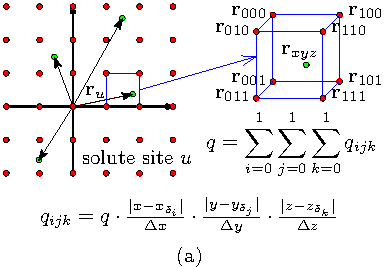
\includegraphics{/Users/lding/Desktop/__M0921/_figure/charge_int}
\par\end{centering}

\caption{Charge density projected onto grids\label{fig:Charge-density-projected}.
(a) Solute. (b) Solvent.}
\end{figure}


\begin{equation}
V_{\mathrm{coul}}(\mathbf{r},\mathbf{\Omega})=\sum_{v}q_{v}V_{q}(\mathbf{r}_{u})
\end{equation}


Poisson solver

Field 
\begin{equation}
E(\mathbf{r})=-\overrightarrow{\nabla}V_{q}(\mathbf{r})
\end{equation}
where $V_{q}(\mathbf{r})$ is ... of unity ...

Local expression of Gauss theorem 
\begin{equation}
\nabla\cdot E(\mathbf{r})=\frac{\rho_{q}(\mathbf{r})}{\varepsilon_{0}}
\end{equation}
therefore

\begin{equation}
\nabla^{2}V_{q}(\mathbf{r})=-\frac{\rho_{q}(\mathbf{r})}{\varepsilon_{0}}
\end{equation}


\begin{equation}
\hat{V}_{q}(\mathbf{k})=\frac{\hat{\rho}_{q}(\mathbf{k})}{\varepsilon_{0}k^{2}}
\end{equation}
where $\hat{V}_{q}(\mathbf{k})$ is the Fourier transform of $V_{q}(\mathbf{r})$.

The Fourier transform, since the Laplacian is a linear operator

\begin{eqnarray}
\nabla^{2}f(\mathbf{r}) & = & \nabla^{2}\int\mathrm{d}\mathbf{k}\hat{f}(k)e^{2\pi i\mathbf{r}\cdot\mathbf{k}}\\
 & = & \int\mathrm{d}\mathbf{k}\hat{f}(k)\nabla^{2}e^{2\pi i\mathbf{r}\cdot\mathbf{k}}\\
 & = & \int\mathrm{d}\mathbf{k}\left(-4\pi^{2}\left|\mathbf{k}\right|^{2}\right)\hat{f}(k)e^{2\pi i\mathbf{r}\cdot\mathbf{k}}
\end{eqnarray}


\begin{equation}
\mathcal{F}\left[\nabla^{2}V_{q}(\mathbf{r})\right]=-4\pi^{2}\left|\mathbf{k}\right|^{2}\hat{V}_{q}(\mathbf{k})
\end{equation}
For Fourier series $-4\pi^{2}\left|\mathbf{k}\right|^{2}$ is the
eigenvalue of laplacian 

\begin{equation}
\mathcal{F}\left[\nabla^{2}V_{q}(\mathbf{r})\right]=\mathcal{F}\left[-\frac{\rho_{q}(\mathbf{r})}{\varepsilon_{0}}\right]=\left(i\mathbf{k}\right)^{2}\hat{V}_{q}(\mathbf{k})=-4\pi\hat{\rho}_{q}(\mathbf{k})
\end{equation}


\begin{equation}
\hat{V}_{\mathrm{Poisson}}(\mathbf{k})=\frac{4\pi\hat{\rho}_{q}(\mathbf{k})}{k^{2}}
\end{equation}



\subsection{Evaluation of $V_{\mathrm{exc}}$}

$V_{\mathrm{exc}}$ is ... of unity {[}{]}

Diople

We define $r=\left\Vert \bm{r}-\bm{r}^{\prime}\right\Vert $, and
$\Delta n\left(\bm{r}\right)=n\left(\bm{r}\right)-n_{0}$, and $n_{0}$
the density of the bulk solvent, e.g., 0.0332891 molecule per $\textrm{\AA}^{3}$
for water.

We also define $n\left(\bm{r}\right)=\int\rho(\bm{r},\boldsymbol{\Omega})\mbox{d}\boldsymbol{\Omega}$.
We have 
\begin{eqnarray}
F_{exc} & = & -\frac{1}{2}k_{B}T\iint\Delta n\left(\boldsymbol{r}\right)\Delta n\left(\boldsymbol{r}^{\prime}\right)c\left(r\right)d\bm{r}d\bm{r}^{\prime},
\end{eqnarray}
Now, we consider the convolution in the right hand side of the equation,
$\gamma\equiv\left(\Delta n*c\right)$, that can be computed much
efficiently than in $O\left(N^{2}\right)$ by fast Fourier transform
in $O\left(N\log N\right)$.

\begin{eqnarray}
\bm{P}\left(\bm{r}\right) & = & \int\bm{p}\rho\left(\bm{r},\bm{\Omega}\right)d\bm{\Omega}
\end{eqnarray}
with $\bm{p}=p\bm{\Omega}$ the dipolar moment of a water molecule.

HRF approximation \citep{Zhao_2011}

Work by Zhao et al.


\ctparttext{This chapter presents a complete theory of the $\mathcal{F}_{\mathrm{exc}}$
evaluation under HRF approximation: 
\[
\mathcal{F}_{\mathrm{exc}}=-\frac{\beta^{-1}}{2}\int\mathrm{d}\mathbf{r_{1}}\mathrm{d}\mathbf{r_{2}}\mathrm{d}\mathbf{\Omega_{1}}\mathrm{d}\mathbf{\Omega_{2}}\Delta\rho(\mathbf{r_{1}},\mathbf{\Omega_{1}})\Delta\rho(\mathbf{r_{2}},\mathbf{\Omega_{2}})c(r_{12},\mathbf{\Omega_{1}},\mathbf{\Omega_{2}})
\]
which is based on previous work of Zhao et al. \citep{Zhao_2011},
where the HRF approximation bas been applied to linear molecules ($\mathbf{\Omega}\equiv(\Theta,\Phi)$).
In this thesis, the method is generated to molecular solvent, using
3 Euler angles, i. e. $\mathbf{\Omega}\equiv(\Theta,\Phi,\Psi)$,
where the computing cost of the original algorithm is no longer reasonable.
Further approximation is therefore made, where the density variable
$\rho(\mathbf{r},\mathbf{\Omega})$ is expended on generalized spherical
harmonics. Theoretically, this approximation gives little loss of
accuracy, but makes a great advantage in computing time and memory
requirement. The prove is shown in the implementation part.\\
\medskip{}
Section \ref{chpt:fft-spatial} describes the FFT treatment for the
spatial convolution in the gradient $\gamma$ of the excess functional
$\mathcal{F}_{\mathrm{exc}}$, which reduces the algorithm complexity
from $O(N^{2})$ to $O(N\log_{2}N)$. A DCF directly issue of Monte
Carlo simulation and solution HNC is used, in both intermolecular
and projection form. To use the intermolecular form, the matrix which
does the transform from laboratory to intermolecular coordinates system
is generalized to molecular case compared to previous work, then interpolation
of zero and first order is involved. To use the projection from, DCF
is reconstructed with all projections. For order of projections $n_{\mathrm{max}}=1$,
the formula of each projections are written explicitly. \\
\medskip{}
Section \ref{chpt:angular-convolution} presents the treatment of
angular convolution. As IEM and MDFT have mathematical equivalence,
an algorithm inspired by the work of Fries \citep{Fries_Patey_1985}
and Blum \citep{Blum_I,Blum_II} for IEM is built for MDFT. In this
algorithm, the density variable $\rho(\mathbf{r},\mathbf{\Omega})$
is expended on generalized spherical harmonics, then rotated onto
intermolecular frame. It is shown that in this form, the OZ equation
is largely simplified.\\
\medskip{}
The solvent properties involved in this thesis are presented in the
next two chapters. Section \ref{chpt:thermodynamic-quantities} presents
some thermodynamic quantities, including the solvation free energy
and its corrections, ... and section \ref{chpt:solvation-structure}
gives some forms of structure that can be preformed, such as the radical
distribution function, radical polarization functions, rotational
invariants expansion, etc.}

\part{Theory: HRF Approximation, For Molecular Solvent}


\chapter{Angular Integration in Excess Functional \label{chpt:fft-spatial}}

As discussed last chapter, the Fourier transform of the excess
functional gradient is:
\begin{equation}
\hat{\gamma}(\mathbf{k},\mathbf{\Omega}_{1})=\int\mathrm{d}\mathbf{\Omega}_{2}\Delta\hat{\rho}(\mathbf{k},\mathbf{\Omega}_{2})\hat{c}(\mathbf{k},\mathbf{\Omega}_{1},\mathbf{\Omega}_{2})\label{eq:gamma-k}
\end{equation}

It should be pointed out that the direct correlation function (\acs{DCF}),
$\hat{c}(\mathbf{k},\mathbf{\Omega}_{1},\mathbf{\Omega}_{2})$, used
as input data in eq. (\ref{eq:gamma-k}) is very memory-costly.
In the previous work \citep{gendre_classical_2009,Zhao_2011,borgis_molecular_2012},
the \acs{DCF} was stocked in the intermolecular form $\hat{c}(k,\boldsymbol{\omega}_{1},\boldsymbol{\omega}_{2})$
to take advantage of an economy of memory, where $(\boldsymbol{\omega}_{1},\boldsymbol{\omega}_{2})\equiv(\cos\theta_{1},\cos\theta_{2},\phi_{12})$,
and the correspondence of $(\mathbf{\Omega}_{1},\mathbf{\Omega}_{2})$
to $(\boldsymbol{\omega}_{1},\boldsymbol{\omega}_{2})$ is calculated
directly in the code. These works adapt well with linear solvents,
but are proven less powerful for molecular solvents such as water.
However, in the case of full Euler angles intermolecular \acs{DCF}
(fig. \ref{fig:coordinate_systems}), 
\begin{equation}
\hat{c}(k,\boldsymbol{\omega}_{1},\boldsymbol{\omega}_{2})\equiv\hat{c}(k,\cos\theta_{1},\cos\theta_{2},\phi,\psi_{1},\psi_{2})
\end{equation}
neither the storage of $\hat{c}(\mathbf{k},\mathbf{\Omega}_{1},\mathbf{\Omega}_{2})$
which is definitively impossible, nor the direct calculation of correspondence
$(\mathbf{\Omega}_{1},\mathbf{\Omega}_{2})$ to $(\boldsymbol{\omega}_{1},\boldsymbol{\omega}_{2})$
due to the increased complexity and resulting cost, can be regarded
as possible solutions. For instance, with a normal setting of $64^{3}$
spatial grid and a Lebedev quadrature of order 2 (14 angles for $\Theta$
and $\Phi$), and 3 $\Psi$-angles, even if the \acs{DCF} is stocked
in simple precision (complex number), it takes $64^{3}\times42^{2}\times4\,\mathrm{bytes}\times2=3.52\mathrm{GB}$,
and for a Lebedev quadrature of order 5 and correspondingly 5 $\Psi$-angles,
it takes $64^{3}\times250^{2}\times4\,\mathrm{bytes}\times2=131\mathrm{GB}$.
As a normal PC has only 4 to 16 GB of RAM, this can cause a memory leak. 

Therefore, two strategies are developed to treat the full \acs{DCF}
case. The first one is a direct extension of the previous work, which
uses the full intermolecular \acs{DCF} with a more complicated angle
correspondence pre-tabulated in the beginning of the implementation.
The other calculates the \acs{DCF} directly from rotational invariant
projections. Here we give a complete discussion of these two strategies.

\begin{figure}[H]
\begin{centering}
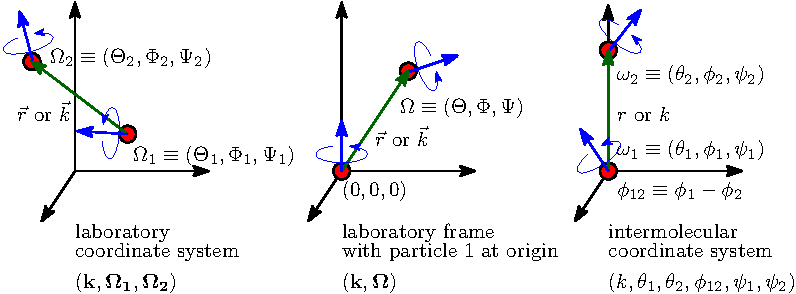
\includegraphics{_figure/coordinate_system}
\par\end{centering}
\caption[Molecules 1 and 2 in different coordinate systems]{Molecules 1 and 2 in different coordinate systems. The laboratory
coordinate system is the system of our grid with a fixed reference
view. When one of the molecules is considered as the reference, e.g.
the solute in the case of $\rho(\mathbf{r},\mathbf{\Omega})$, only
one $\mathbf{\Omega}$ needs to be described. For the intermolecular
frame, in $\mathbf{r}$-space, the $z$ axis is oriented along the
vector $\mathbf{r}_{12}=\mathbf{r}_{2}-\mathbf{r}_{1}$, or in $\mathbf{k}$-space
along the vector $\mathbf{k}$. An orientation $\mathbf{\Omega}\equiv(\Theta,\Phi,\Psi)$
in laboratory frame corresponds to $\boldsymbol{\omega}\equiv(\theta,\phi,\psi)$
in intermolecular frame.\label{fig:coordinate_systems}}
\end{figure}


\section{Using full intermolecular DCF}

For the full \acs{DCF} in intermolecular coordinates system, $\hat{c}(k,\boldsymbol{\omega}_{1},\boldsymbol{\omega}_{2})$,
only 6 variables are needed instead of 9 for $\hat{c}(\mathbf{k},\mathbf{\Omega}_{1},\mathbf{\Omega}_{2})$,
and the storage is considerably reduced. The transformation from $\hat{c}(\mathbf{k},\mathbf{\Omega}_{1},\mathbf{\Omega}_{2})$
to $\hat{c}(k,\boldsymbol{\omega}_{1},\boldsymbol{\omega}_{2})$ relies
on the correspondence $\boldsymbol{\omega}(\mathbf{k},\mathbf{\Omega})\equiv(\cos\theta,\phi,\psi)$,
which here is pre-calculated as a table of data.

Finding $\boldsymbol{\omega}$ from $\mathbf{\Omega}$ amounts to
defining the correspondence between the rotation matrices of the two
coordinate systems. The rotation matrix $\mathbf{\hat{R}}_{\mathbf{\Omega}}$
that rotates the solvent molecule from $\mathbf{I}$ to its orientation
$\mathbf{\hat{R}}_{\mathbf{\Omega}}$
\begin{equation}
\mathbf{\hat{R}}_{\mathbf{\Omega}}\mathbf{I}=\mathbf{\hat{R}}_{\mathbf{\Omega}}
\end{equation}
can be expressed by 3 rotation operations $\mathbf{\hat{R}}_{\Phi}$,
$\mathbf{\hat{R}}_{\Theta}$, and $\mathbf{\hat{R}}_{\Psi}$ which
rotate along $x$-$y$-$z$ axes (the same convention as defined in
Messiah \citep{Messiah} and Gray-Gubbins \citep{Gray-Gubbins}):
\begin{align}
\mathbf{\hat{R}}_{\mathbf{\Omega}} & =\left[\begin{array}{ccc}
R_{xx} & R_{xy} & R_{xz}\\
R_{yx} & R_{yy} & R_{yz}\\
R_{zx} & R_{zy} & R_{zz}
\end{array}\right]\\
 & =\left[\begin{array}{ccc}
\cos\Phi & -\sin\Phi & 0\\
\sin\Phi & \cos\Phi & 0\\
0 & 0 & 1
\end{array}\right]\left[\begin{array}{ccc}
\cos\Theta & 0 & \sin\Theta\\
0 & 1 & 0\\
-\sin\Theta & 0 & \cos\Theta
\end{array}\right]\left[\begin{array}{ccc}
\cos\Psi & -\sin\Psi & 0\\
\sin\Psi & \cos\Psi & 0\\
0 & 0 & 1
\end{array}\right]\nonumber \\
 & =\footnotesize\left[\begin{array}{ccc}
\cos\Phi\cos\Theta\cos\Psi-\sin\Phi\sin\Psi & -\cos\Phi\cos\Theta\sin\Psi-\sin\Phi\cos\Psi & \cos\Phi\sin\Theta\\
\sin\Phi\cos\Theta\cos\Psi+\cos\Phi\sin\Psi & -\sin\Phi\cos\Theta\sin\Psi+\cos\Phi\cos\Psi & \sin\Phi\sin\Theta\\
-\sin\Theta\cos\Psi & \sin\Theta\sin\Psi & \cos\Theta
\end{array}\right]\nonumber 
\end{align}
\begin{figure}[b]
\centering{}%
\begin{minipage}[b][1\totalheight][t]{0.55\columnwidth}%
\begin{center}
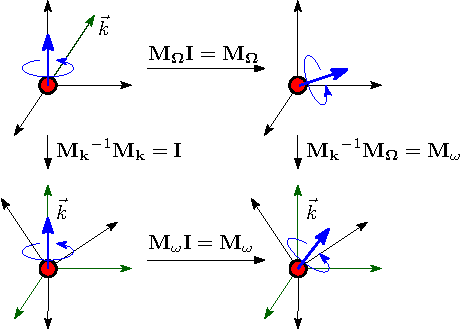
\includegraphics{_figure/rotation_matrix}\caption{Rotation matrices\label{fig:rotation-matrices}}
\par\end{center}%
\end{minipage}%
\begin{minipage}[b][1\totalheight][t]{0.4\columnwidth}%
\begin{center}
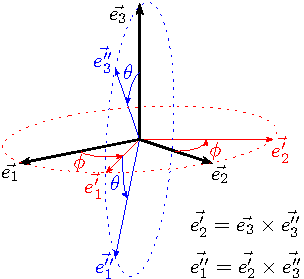
\includegraphics{_figure/rotation_matrix_k}
\par\end{center}
\caption{Rotation to k-frame\label{fig:rotation}}
%
\end{minipage}
\end{figure}

As shown in fig. \ref{fig:rotation-matrices}, the rotation matrix
to transform the \acs{DCF} from the intermolecular coordinates to
laboratory coordinates $\mathbf{\hat{R}}_{\boldsymbol{\omega}}$ can
be written as:
\begin{equation}
\mathbf{\hat{R}}_{\boldsymbol{\omega}}=\mathbf{\hat{R}}_{\mathbf{k}}^{-1}\mathbf{\hat{R}}_{\mathbf{\Omega}}\label{eq:rot-matrix}
\end{equation}
with the rotation matrix related to $\mathbf{k}$ vector:
\begin{equation}
\mathbf{\hat{R}}_{\mathbf{k}}^{-1}=\left[\begin{array}{ccc}
\cos\theta_{k}\cos\phi_{k} & \cos\theta_{k}\sin\phi_{k} & -\sin\theta_{k}\\
-\sin\phi_{k} & \cos\phi_{k} & 0\\
\sin\theta_{k}\cos\phi_{k} & \sin\theta_{k}\sin\phi_{k} & \cos\theta_{k}
\end{array}\right]
\end{equation}

Here we fix $\psi_{k}=0$. $\theta_{k}$ and $\phi_{k}$ are calculated
from Cartesian coordinates ($k_{x}$, $k_{y}$, $k_{z}$). In
extreme cases where we cannot define $\theta_{k}$ (for $\left\Vert \mathbf{k}\right\Vert =0$)
and $\phi_{k}$ (for $k_{x}^{2}+k_{y}^{2}=0$), we can arbitrarily
fix those angles to zero.

A faster way to find the rotation matrix of $\mathbf{k}$, avoiding
the evaluation of trigonometric functions, is shown in figure \ref{fig:rotation},
where the matrix can be calculated by the cross products of basis
vectors from $z$ axis and $\mathbf{k}$ vector ($\mathbf{k}=\mathbf{e}_{3}^{''}$):
\begin{equation}
\left[\begin{array}{ccc}
\mathbf{e}_{1}^{''} & \mathbf{e}_{2}^{'} & \mathbf{e}_{3}^{''}\end{array}\right]=\left[\begin{array}{ccc}
\mathbf{e}_{1} & \mathbf{e}_{2} & \mathbf{e}_{3}\end{array}\right]\mathbf{\hat{R}_{k}}=\mathbf{\hat{R}_{k}}
\end{equation}

The two ways to calculate $\mathbf{k}$ differ only in the case of
$\hat{\mathbf{k}}=\left[\begin{array}{ccc}
0 & 0 & -1\end{array}\right]^{T}$, where one is the inverse of the other. This is due to the different
definitions of $\phi_{k}$ ($0$ or $\pi$ when $\overrightarrow{k'_{z}}$
superposes with $\overrightarrow{k_{z}}$) in the two cases. Tests
have shown that it has no influence on the final result of the excess
functional evaluation.

The elements of $\mathbf{\hat{R}}_{\boldsymbol{\omega}}$ can be calculated
according to eq. (\ref{eq:rot-matrix}), which possesses the form:
\begin{align}
\mathbf{\hat{R}}_{\boldsymbol{\omega}} & =\left[\begin{array}{ccc}
u_{x} & v_{x} & w_{x}\\
u_{y} & v_{y} & w_{y}\\
u_{z} & v_{z} & w_{z}
\end{array}\right]\\
 & =\footnotesize\left[\begin{array}{ccc}
\cos\phi\cos\theta\cos\psi-\sin\phi\sin\psi & -\cos\phi\cos\theta\sin\psi-\sin\phi\cos\psi & \cos\phi\sin\theta\\
\sin\phi\cos\theta\cos\psi+\cos\phi\sin\psi & -\sin\phi\cos\theta\sin\psi+\cos\phi\cos\psi & \sin\phi\sin\theta\\
-\sin\theta\cos\psi & \sin\theta\sin\psi & \cos\theta
\end{array}\right]\nonumber 
\end{align}

The angles $\boldsymbol{\omega}$ are thus found as:
\begin{eqnarray}
\cos\theta & = & w_{z}\nonumber \\
\phi & = & \arccos(w_{x}/(w_{x}^{2}+w_{y}^{2})^{\frac{1}{2}})\label{eq:omega}\\
\psi & = & \arccos(-u_{z}/(u_{z}^{2}+v_{z}^{2})^{\frac{1}{2}})\nonumber 
\end{eqnarray}

The resulting angles are between normal intervals, $\cos\theta\in\left[-1,1\right]$,
$\phi\in\left[0,2\pi\right]$. As water possesses $\mathrm{C}_{2v}$
symmetry, we take $\psi\in\left[0,\pi\right]$. 

Here the \acs{DCF} $c(k,\boldsymbol{\omega}_{1},\boldsymbol{\omega}_{2})\equiv c(k,\cos\theta_{1},\cos\theta_{2},\phi_{12},\psi_{1},\psi_{2})$
is stored in a discrete set of angles for each value of $k$ (typically
$(8,8,8,8,8)$ in the case of water, which uses the symmetries in
$\mathsection$\ref{subsec:Symmetric-dcf} to reduce the number of
$\phi$ and $\psi$ by two) such that the correspondence from $(\mathbf{\Omega}_{1},\mathbf{\Omega}_{2})$
to $(\boldsymbol{\omega}_{1},\boldsymbol{\omega}_{2})$ usually falls
between angular grid points of the intermolecular grid. An interpolation
can be done at different orders: zeroth order interpolation, which
directly takes the nearest point, or linear interpolation.

\subsection{Zero-order interpolation of DCF\label{subsec:Zero-order-interpolation-of}}

At this order, for each possible value of $\mathbf{k}$ and $\mathbf{\Omega}$,
the corresponding $\cos\theta$ and $\psi$ which relate to a single
solvent molecule are stored as an index (single precision integer),
which gives the nearest angle in a pre-defined table:
\begin{equation}
\begin{array}{l}
i_{\cos\theta}=\left\lfloor (\cos\theta+1)(n_{\cos\theta}/2)\right\rfloor +1\\
i_{\psi}=\mathrm{mod}(\left\lfloor \psi(n_{\psi}/\pi)\right\rfloor ,n_{\psi})+1
\end{array}
\end{equation}
where $\left\lfloor f\right\rfloor $ is the floor function. For the
angle $\phi$ which relates to two solvent molecules, the operation
$\phi=\phi_{1}-\phi_{2}$ introduces a double error when integer indices
are used, as shown in figure \ref{fig:diff_phi}.

\begin{figure}[h]
\begin{centering}
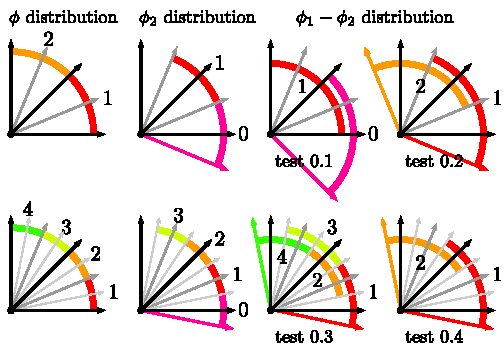
\includegraphics{_figure/diff_phi}
\par\end{centering}
\caption[$\phi_{1}-\phi_{2}$ distribution]{$\phi_{1}-\phi_{2}$ distribution: Test 0.1 is the direct subtraction
of $\phi$ established in the same way with $\theta$ and $\psi$,
as shown in the top first schema. Test 0.2 tabulates $\phi_{2}$ by
taking the nearest point in another manner, as shown in the second
schema. In test 0.3-0.4, all $\phi$ or only $\phi_{2}$ is doubled.\label{fig:diff_phi}}
\end{figure}

In the actual implementation, as an integer takes 4 bytes and a real
takes 8 bytes, there is no profit to tabulate $\phi$ as an integer two
times, thus $\phi$ is stored directly in real.

\subsection{Linear interpolation of DCF\label{subsec:Linear-interpolation-of}}

At this order, $\boldsymbol{\omega}(\mathbf{k},\mathbf{\Omega})$
is stored in double precision. All angles are stored in real number form,
and the corresponding \acs{DCF} is calculated as
\begin{equation}
c(\omega)=w_{0}c(\omega_{0})+w_{1}c(\omega_{1})
\end{equation}
where $w_{0}=\dfrac{\omega_{1}-\omega}{\omega_{1}-\omega_{0}}$ and
$w_{1}=\dfrac{\omega-\omega_{0}}{\omega_{1}-\omega_{0}}$. \marginpar{$w$ is the weight, and $\omega$ is the angle set.}Here
$\omega$ is one of the 5 dimensions in $\tilde{\boldsymbol{\omega}}(\mathbf{k},\mathbf{\Omega}_{1},\mathbf{\Omega}_{2})\equiv(\cos\theta_{1},\cos\theta_{2},\phi,\psi_{1},\psi_{2})$,
$\omega_{0}$ and $\omega_{1}$ are the 2 nearest value points, while
other variables are fixed. If we express the weight for each dimension
as $w_{n_{i}}^{i}$ where $i=1,2,3,4,5$ is the $i$th variable, the
total equation with 5 variables is:
\begin{equation}
c(\tilde{\boldsymbol{\omega}})=\left[\sum_{n_{1}=0}^{1}\sum_{n_{2}=0}^{1}\sum_{n_{3}=0}^{1}\sum_{n_{4}=0}^{1}\sum_{n_{5}=0}^{1}\left(\prod_{i}^{5}w_{n_{i}}^{i}c(\tilde{\boldsymbol{\omega}}_{n_{1},n_{2},n_{3},n_{4},n_{5}})\right)\right]\label{eq:interpolation}
\end{equation}

These two equations are available for both interpolation and extrapolation,
where the latter applies, e.g., for $\cos\theta_{1}$ and $\cos\theta_{2}$. 

An error evaluation of the two strategies of interpolation presented
in $\mathsection$\ref{subsec:Zero-order-interpolation-of} and $\mathsection$\ref{subsec:Linear-interpolation-of}
is shown in appendix \ref{chpt:error-evaluation-interpolation-DCF}.
Results demonstrate that the linear interpolation scheme is absolutely
essential. On the other hand, as seen in eq. (\ref{eq:interpolation}),
it is computationally much more expensive than the simple histogram
scheme as it requires $2^{5}=32$ times the number of operations.

\section{Direct calculation of DCF from rotational invariant projections}

Another strategy to calculate $\hat{c}(\mathbf{k},\mathbf{\Omega}_{1},\mathbf{\Omega}_{2})$
is to use the \acs{DCF} expressed in terms of rotational invariant
projections, which takes far less memory than in the intermolecular
function form thanks to their angular independence and symmetric properties. 

\subsection{Using projections in the form of $\hat{c}_{\mu\nu}^{mnl}(k)$\label{subsec:Using-projections-in}}

As described by Blum \citep{Blum_I}, $\hat{c}(\mathbf{k},\mathbf{\Omega}_{1},\mathbf{\Omega}_{2})$
can be expanded as
\begin{equation}
\hat{c}(\mathbf{k},\mathbf{\Omega}_{1},\mathbf{\Omega}_{2})=\sum_{mnl\mu\nu}\hat{c}_{\mu\nu}^{mnl}(k)\Phi_{\mu\nu}^{mnl}(\mathbf{\hat{k}},\mathbf{\Omega}_{1},\mathbf{\Omega}_{2})
\end{equation}
where $\Phi_{\mu\nu}^{mnl}(\mathbf{\hat{k}},\mathbf{\Omega}_{1},\mathbf{\Omega}_{2})$
are rotational invariants that depend on both the spatial and angular
coordinates of the two particles (detailed in appendix \ref{chpt:rotational-invariant-expansion}).

For projections of order $n_{\mathrm{max}}=1$ ($n,m\leq1$), the
\acs{DCF} can be expressed in very simple form. Only 4 projections
$\hat{c}^{mnl}(k)$ are independent: $\hat{c}_{\mathrm{S}}\equiv\hat{c}^{000}$,
$\hat{c}_{\mathrm{\Delta}}\equiv\hat{c}^{110}$, $\hat{c}_{\mathrm{D}}\equiv\hat{c}^{112}$
and $\hat{c}^{011}=-\hat{c}^{101}$, with the corresponding rotational
invariants expressed below both in laboratory and intermolecular frames:
\begin{align}
\Phi^{000} & =1\nonumber \\
\Phi^{011} & =i\mathbf{k}\cdot\mathbf{\Omega}_{1}=i\cos\theta_{1}\nonumber \\
\Phi^{101} & =i\mathbf{k}\cdot\mathbf{\Omega}_{2}=i\cos\theta_{2}\nonumber \\
\Phi^{110} & =-\sqrt{3}\mathbf{\Omega}_{1}\cdot\mathbf{\Omega}_{2}=-\sqrt{3}(\sin\theta_{1}\sin\theta_{2}\cos\phi_{12}+\cos\theta_{1}\cos\theta_{2})\nonumber \\
\Phi^{112} & =\sqrt{\frac{3}{10}}\left[3(\mathbf{k}\cdot\mathbf{\Omega}_{1})(\mathbf{k}\cdot\mathbf{\Omega}_{2})-\mathbf{\Omega}_{1}\cdot\mathbf{\Omega}_{2}\right]\\
 & =\sqrt{\frac{3}{10}}\left(2\cos\theta_{1}\cos\theta_{2}-\sin\theta_{1}\sin\theta_{2}\cos\phi_{12}\right)\nonumber 
\end{align}
where the orientations in laboratory frame $\mathbf{\Omega}$ are
here expressed as an orientational vector $\mathbf{\Omega}=(\sin\Theta\cos\Phi,\sin\Theta\sin\Phi,\cos\Theta)$
in the Cartesian coordinate system. 

To express the \acs{DCF} at higher orders, the number of \acs{FE}
needed for $\Phi_{\mu\nu}^{mnl}(\mathbf{\hat{k}},\mathbf{\Omega}_{1},\mathbf{\Omega}_{2})$
becomes huge and the \acs{DCF} should be calculated in intermolecular
frame as indicated below.

\subsection{Using projections in the form of $\hat{c'}_{\mu\nu,\chi}^{mn}(k)$\label{subsec:Using-projections-in-1}}

Compared to the expression of $\Phi_{\mu\nu}^{mnl}(\mathbf{\hat{k}},\mathbf{\Omega}_{1},\mathbf{\Omega}_{2})$
in laboratory frame (eq. (\ref{eq:definition_rot_invar})), its intermolecular
form has far fewer terms (eq. (\ref{eq:phi_local})), such that
\begin{equation}
\hat{c}(k,\boldsymbol{\omega}_{1},\boldsymbol{\omega}_{2})=\frac{1}{2l+1}\sum_{mn\mu\nu\chi}\hat{c'}_{\mu\nu,\chi}^{mn}(k)r_{\chi\mu}^{m}(\theta_{1})r_{\underline{\chi}\nu}^{n}(\theta_{2})e^{-i\chi(\phi_{12}\equiv\phi_{1}-\phi_{2})}e^{-i\mu\psi_{1}}e^{-i\nu\psi_{2}}\label{eq:dcf-exact}
\end{equation}
where $r$ is the generalized Legendre polynomial, $m,n\leq n{}_{\mathrm{max}}$,
$\left|\mu\right|\leq m$, $\left|\nu\right|\leq n$, and $\chi\in\left[-\mathrm{min}(m,n),\mathrm{min}(m,n)\right]$;
$\underline{\chi}=-\chi$.

$r_{\chi\mu}^{m}(\theta)$, $e^{-i\chi\phi}(\phi)$ and $e^{-i\mu\psi}(\psi)$
can be separately pre-tabulated for each given $\mathbf{k}$, to avoid
repetitive evaluation of each term.

Eq. (\ref{eq:dcf-exact}) replaces the interpolation of eq. (\ref{eq:interpolation})
by an exact formula, and it requires the projections $\hat{c}_{\mu\nu,\chi}^{mn}(k)$
to be stored in memory rather than the full angular representation
$\hat{c}(k,\boldsymbol{\omega}_{1},\boldsymbol{\omega}_{2})$. It
also requires the passage from orientations in laboratory frame to
orientations in intermolecular frame, i.e. use of the formulae (\ref{eq:omega})
for each $\mathbf{k}$ vector.



\chapter{Angular Convolution, A Better Algorithm\label{chpt:angular-convolution}}

In section \ref{chpt:fft-spatial}, the spatial convolution is treated
by FFT thanks to the transitional invariance that leads to $\mathbf{r_{12}}=\mathbf{r_{1}}-\mathbf{r_{2}}$.
However, as the angular grid is not homogeneous, the relative coordinates
of two angles cannot be simply represented $\mathbf{\Omega_{12}}=\mathbf{\Omega_{1}}-\mathbf{\Omega_{2}}$,
therefore we cannot take advantage of the convolution property shown
in eq. (\ref{eq:convolution-1}-\ref{eq:convolution-2}). In other
hand, these two-particle quantities also have rotational invariance.
Proposed by Blum \citep{Blum_I,Blum_II} and used by Fries and Patey
\citep{Fries_Patey_1985}, a rotational invariant expansion technic
reduces the molecular Ornstein-Zernike (MOZ) equation into smaller
irreducible matrix equations. As there is an mathematical equivalence
between IEM and MDFT (section \ref{chpt:mdft}), where eq. (\ref{eq:gamma-k})
can be regarded as the molecular OZ equation, this formalism can be
also applied to MDFT.


\section{Angular convolution using Blum's reduction}

To build a relation between the irreducible form of the molecular
OZ equation deduced by Blum (detailed in section \ref{chpt:iem})
\marginpar{Here the projections $F_{\mu\nu,\chi}^{mn}$ is defined as eq. (appendix)
with symmetries eq. (appendix).\textcolor{red}{{} It's mathematically
identical with {[}ref{]} but using $R_{\mu'\mu}^{m}=D_{\mu'\mu}^{m*}$.}} 
\begin{equation}
\hat{\gamma'}_{\lambda\mu,\chi}^{lm}(k)=\sum_{n=0}^{n_{\mathrm{max}}}\sum_{\nu=-n}^{n}\left(-\right){}^{\chi+\nu}\Delta\hat{\rho'}_{\lambda\underline{\nu},\chi}^{ln}(k)\hat{c'}_{\mu\nu,\chi}^{mn}(k)\label{eq:Blum-reduced-OZ}
\end{equation}
and the MDFT, a generalized spherical harmonic transform (GSHT) treatment
is proposed by Luc Belloni, developing the functional gradient $\hat{\gamma}$
and the density $\hat{\rho}$ in eq. (\ref{eq:gamma-k}) on Wigner
generalized spherical harmonics (GSH):
\begin{equation}
\hat{\gamma}(\mathbf{k},\mathbf{\Omega_{1}})=\sum_{m\mu'\mu}f_{m}\hat{\gamma}_{\mu'\mu}^{m}(\mathbf{k})R_{\mu'\mu}^{m}(\mathbf{\Omega_{1}})\label{eq:gamma-projection}
\end{equation}
\begin{equation}
\Delta\hat{\rho}(\mathbf{k},\mathbf{\Omega_{2}})=\sum_{n\nu'\nu}f_{n}\Delta\hat{\rho}_{\nu',\nu}^{n}(\mathbf{k})R_{\nu',\nu}^{n}(\mathbf{\Omega_{2}})\label{eq:delta-rho-projection}
\end{equation}
where $0\leq m\leq m_{\mathrm{max}}$, $\left|\mu'\right|,\left|\mu\right|<m$
and $\left|\nu'\right|,\left|\nu\right|<n$. $f_{m}=\left(2m+1\right)^{\frac{1}{2}}$
is the normalization factor (according to Luc's definition).

The DCF can also be expended on rotational invariants \citep{Blum_I},
with the normalization factors according to Luc's definition:
\begin{equation}
\hat{c}(k,\mathbf{\Omega_{1}},\mathbf{\Omega_{2}})=\sum_{mnl\mu\nu}f_{m}f_{n}\hat{c}_{\mu\nu}^{mnl}(k)\sum_{\mu'\nu'\lambda'}\left(\begin{array}{ccc}
m & n & l\\
\mu' & \nu' & \lambda'
\end{array}\right)R_{\mu'\mu}^{m}(\mathbf{\Omega_{1}})R_{\nu'\nu}^{n}(\mathbf{\Omega_{2}})R_{\lambda'0}^{l}(\hat{\mathbf{k}})\label{eq:c-projection}
\end{equation}


As GSH possess orthogonality eq. (\ref{eq:gsh-orthogonality}) and
symmetry eq. (\ref{eq:symm-gsh-1}), eq. (\ref{eq:gamma-k}) can be
rewritten by (\ref{eq:gamma-projection}, \ref{eq:delta-rho-projection},
\ref{eq:c-projection}), which gives
\begin{equation}
\hat{\gamma}_{\mu'\mu}^{m}(\mathbf{k})=\sum_{nl\nu}\hat{c}_{\mu\nu}^{mnl}(k)\sum_{\nu'\lambda'}\left(-\right){}^{\nu'+\nu}\Delta\hat{\rho}_{\underline{\nu'}\underline{\nu}}^{n}(\mathbf{k})\left(\begin{array}{ccc}
m & n & l\\
\mu' & \nu' & \lambda'
\end{array}\right)R_{\lambda'0}^{l}(\hat{\mathbf{k}})\label{eq:im}
\end{equation}
thus the OZ equation is expended on GSHs and rotational invariants.

It should be noticed that eq. (\ref{eq:im}) is reducible. Blum's
$\chi$-transform defines\citep{Blum_II} 
\begin{equation}
\hat{c'}_{\mu\nu,\chi}^{mn}(k)=\sum_{l}\left(\begin{array}{ccc}
m & n & l\\
\chi & -\chi & 0
\end{array}\right)\hat{c}_{\mu\nu}^{mnl}(k)
\end{equation}
\marginpar{$\hat{c'}_{\mu\nu,\chi}^{mn}(k)$ is well the invariant in eq. (\ref{eq:Blum-reduced-OZ}).}
\begin{equation}
\hat{c}_{\mu\nu}^{mnl}(k)=\left(2l+1\right)\sum_{\chi}\left(\begin{array}{ccc}
m & n & l\\
\chi & -\chi & 0
\end{array}\right)\hat{c'}_{\mu\nu,\chi}^{mn}(k)\label{eq:c-p}
\end{equation}


Invariants of form $F_{\mu\nu,\chi}^{mn}(k)$ have a very simple relation
with its combined function $F(k,\boldsymbol{\omega_{1}},\boldsymbol{\omega_{2}})$
in intermolecular coordinate system (eq. (\ref{eq:local-forward},
\ref{eq:local_backward})). In MDFT formalism, the projections of
$\hat{\gamma}$ and $\hat{\rho}$ in local frame ($\boldsymbol{\omega_{i}}=\hat{\mathbf{k}}\mathbf{\Omega_{i}}$)
are
\begin{equation}
\hat{\gamma'}(\mathbf{k},\boldsymbol{\omega_{1}})=\sum_{m\chi\mu}f_{m}\hat{\gamma'}_{\chi\mu}^{m}(\mathbf{k})R_{\chi\mu}^{m}(\boldsymbol{\omega_{1}})\label{eq:gamma-projection-local}
\end{equation}
\begin{equation}
\Delta\hat{\rho'}(\mathbf{k},\boldsymbol{\omega_{2}})=\sum_{n\chi\nu}f_{n}\Delta\hat{\rho'}_{\chi\nu}^{n}(\mathbf{k})R_{\chi\nu}^{n}(\mathbf{\boldsymbol{\omega_{2}}})\label{eq:delta-rho-projection-local}
\end{equation}
and with the rotation formula of GSH (eq. (\ref{eq:gsh-rotation})),
we have 
\begin{equation}
\hat{\gamma'}_{\chi\mu}^{m}(\mathbf{k})=\sum_{\mu'}\hat{\gamma}_{\mu'\mu}^{m}(\mathbf{k})R_{\mu'\chi}^{m}(\hat{\mathbf{k}})\label{eq:gamma-p}
\end{equation}
\begin{equation}
\Delta\hat{\rho}_{\underline{\nu'}\underline{\nu}}^{n}(\mathbf{k})=\sum_{\chi}\Delta\hat{\rho'}_{\chi\underline{\nu}}^{n}(\mathbf{k})R_{\underline{\nu'}\chi}^{n*}(\hat{\mathbf{k}})=\sum_{\chi}\Delta\hat{\rho'}_{\chi\underline{\nu}}^{n}(\mathbf{k})\left(-\right){}^{\chi+\nu'}R_{\nu'\underline{\chi}}^{n}(\hat{\mathbf{k}})\label{eq:rho-p}
\end{equation}


Using eq. (\ref{eq:gamma-p}), (\ref{eq:im}), eq. (\ref{eq:rho-p}),
eq. (\ref{eq:c-p}) and GSH products relation eq. (\ref{eq:gg.a91})
and 3j-symbol orthogonality eq. (\ref{eq:3j-orthogonality}), we deduce
that
\begin{equation}
\hat{\gamma'}_{\chi\mu}^{m}(\mathbf{k})=\sum_{n\nu}\left(-\right){}^{\chi+\nu}\hat{c'}_{\mu\nu,\chi}^{mn}(k)\Delta\hat{\rho'}_{\chi\underline{\nu}}^{n}(\mathbf{k})\label{eq:gamma-blum}
\end{equation}


Eq. (\ref{eq:gamma-blum}) is mathematically identical to eq. (\ref{eq:Blum-reduced-OZ}),
as \textcolor{red}{(to be verified with patient...)}

\begin{equation}
\hat{\gamma'}_{\chi\mu}^{m}(\mathbf{k})=\sum_{l\lambda}\hat{\gamma'}_{\lambda\mu,\chi}^{lm*}(k)R_{\chi\lambda}^{l}(\hat{\mathbf{k}})
\end{equation}
\begin{equation}
\hat{\rho'}_{\chi\underline{\nu}}^{n}(\mathbf{k})=\sum_{l\lambda}\Delta\hat{\rho'}_{\lambda\underline{\nu},\chi}^{ln*}(k)R_{\chi\lambda}^{l}(\hat{\mathbf{k}})
\end{equation}


And in this way, the integral of the angular part in eq. (\ref{eq:gamma-k})
is reduced to a sum of a few terms.

Table \ref{tab:FE-of-OZ} shows some parameters linking to computing
cost of different algorithms. It shows that the expansion en GSH (eq.
(\ref{eq:im})) projections doesn't gives an enormous reduction of
FE comparing to its 6D function form (eq. (\ref{eq:gamma-k})), but
after the Blum's $\chi$-transform, the OZ function is largely reduced.
As the spatial convolution takes advantage of the transitional invariance
$r_{12}$, the $\chi$-transform in fact makes use of the rotational
invariance.

\begin{table}[h]
\begin{centering}
\begin{tabular*}{1\textwidth}{@{\extracolsep{\fill}}ccccccc}
\toprule 
{\footnotesize{}$m_{\mathrm{max}}$} & {\footnotesize{}0} & {\footnotesize{}1} & {\footnotesize{}2} & {\footnotesize{}3} & {\footnotesize{}4} & {\footnotesize{}5}\tabularnewline
\midrule
{\footnotesize{}$N_{\Theta}$} & {\footnotesize{}1} & {\footnotesize{}2} & {\footnotesize{}3} & {\footnotesize{}4} & {\footnotesize{}5} & {\footnotesize{}6}\tabularnewline
{\footnotesize{}$N_{\mathrm{ang}}$ (Gauss-Legendre)} & {\footnotesize{}1 (1)} & {\footnotesize{}18 (6)} & {\footnotesize{}75 (45)} & {\footnotesize{}196 (84)} & {\footnotesize{}405 (225)} & {\footnotesize{}726 (330)}\tabularnewline
{\footnotesize{}$N_{\mathrm{ang}}$ (Lebedev$\times\psi$)} & {\footnotesize{}1 (1)} & {\footnotesize{}18 (6)} & {\footnotesize{}70 (42)} & {\footnotesize{}182 (78)} & {\footnotesize{}342 (190)} & {\footnotesize{}550 (250)}\tabularnewline
{\footnotesize{}$N_{\mathrm{proj}}$ } & {\footnotesize{}1 (1)} & {\footnotesize{}10 (4)} & {\footnotesize{}35 (19)} & {\footnotesize{}84 (40)} & {\footnotesize{}165 (85)} & {\footnotesize{}286 (140)}\tabularnewline
{\footnotesize{}FE for eq. (\ref{eq:gamma-k})} & {\footnotesize{}1 (1)} & {\footnotesize{}324 (36)} & {\footnotesize{}5625 (2025)} & {\footnotesize{}38416 (7056)} & {\footnotesize{}164025 (50625)} & {\footnotesize{}527076 (108900)}\tabularnewline
\textcolor{red}{\footnotesize{}FE for eq. (\ref{eq:im})} & \textcolor{red}{\footnotesize{}1 (1)} & \textcolor{red}{\footnotesize{}262 (6)} & \textcolor{red}{\footnotesize{}4787 (483)} & \textcolor{red}{\footnotesize{}36588 (1932)} & \textcolor{red}{\footnotesize{}175989 (13157)} & \textcolor{red}{\footnotesize{}633490 (36882)}\tabularnewline
{\footnotesize{}FE for eq. (\ref{eq:gamma-blum})} & {\footnotesize{}1 (1)} & {\footnotesize{}34 (6)} & {\footnotesize{}259 (75)} & {\footnotesize{}1092 (252)} & {\footnotesize{}3333 (877)} & {\footnotesize{}8294 (2002)}\tabularnewline
\bottomrule
\end{tabular*}
\par\end{centering}

\caption[Number of FE needed by OZ equation of different form]{Number of FE needed by OZ equation of different form for arbitrary
solvent (outside the parentheses) and solvent possessing $\mathrm{C}_{2v}$
symmetry (inside the parentheses)\label{tab:FE-of-OZ}}
\end{table}



\section{Fast generalized spherical harmonic transform}

In the angular convolution algorithm above, the OZ equation is reduced
to a few function evaluations by taking advantage of the orthogonality
and symmetries of rotation invariants. It's analogue to the treatment
of convolution with FFT for spatial grid, in which the generalized
spherical harmonics transform (GSHT) is used as an alternative of
FFT for inhomogeneous grid, and it \textit{a priori }should be fast.

The FGHST provides a forward-backward transform between a general
angular function $F(\mathbf{\Omega})\equiv F(\cos\Theta,\Phi,\Psi)$
and its projections $F_{\mu'\mu}^{m}$ ($\left|\mu'\right|,\left|\mu\right|\leq m$)
\begin{equation}
F_{\mu'\mu}^{m}=\frac{f_{m}}{8\pi^{2}}\int\mathrm{d}\mathbf{\Omega}F(\mathbf{\Omega})R_{\mu'\mu}^{m*}(\mathbf{\Omega})\begin{array}{c}
\mathrm{(forward)}\end{array}\label{eq:GSHT_forward}
\end{equation}
\begin{equation}
F(\mathbf{\Omega})=\sum_{m,\mu',\mu}f_{m}F_{\mu'\mu}^{m}R_{\mu'\mu}^{m}(\mathbf{\Omega})\begin{array}{c}
\mathrm{(backward)}\end{array}\label{eq:GSHT_backward}
\end{equation}
where $f_{m}=\left(2m+1\right)^{\frac{1}{2}}=\left\Vert R_{\mu'\mu}^{m}\right\Vert ^{-1}$
is the normalization factor, and $R_{\mu'\mu}^{m}(\mathbf{\Omega})$
is the Wigner generalized spherical harmonics (Appendix \textcolor{red}{{[}Ref{]}})
being defined as
\begin{equation}
R_{\mu'\mu}^{m}(\mathbf{\Omega})=r_{\mu'\mu}^{m}(\Theta)e^{-i(\mu'\Phi+\mu\Psi)}
\end{equation}
which form a complete orthogonal set.


\subsection{Equivalence of order in angular quadratures and projections}

Suppose that $F(\mathbf{\Omega})$ is a polynomial of $\cos\Theta$,
$\cos\Phi$ and $\cos\Psi$ of order $n$, ($n+1$ polynomial terms).
To expand completely this function as shown in equation (\ref{eq:GSHT_backward}),
at least $n_{\mathrm{max}}=n$ is needed. Then to evaluate exactly
the integration in equation (\ref{eq:GSHT_forward}), at least $n+1$
for $\cos\Theta$ (Gauss-Legendre grid), $2n+1$ for $\Phi$ (equal-spaced
grid), $2n+1$ for $\Psi$ (equal-spaced grid) points of angular grid
are needed (c. f. appendix \ref{chpt:equivalence-of-quadrature-projection-order}).
In the case of water who possesses a $\mathrm{C}_{2}$ symmetry $F(\Psi+\pi)=F(\Psi)$,
only projections of even $\mu$ is nonzero
\begin{equation}
F_{\mu}=\int\mathrm{d}\Psi F(\Psi)e^{i\mu\Psi}=\int\mathrm{d}(\Psi+\pi)F(\Psi+\pi)e^{i\mu(\Psi+\pi)}=e^{i\mu\pi}\int\mathrm{d}\Psi F(\Psi)e^{i\mu\Psi}=e^{i\mu\pi}F_{\mu}
\end{equation}
\begin{equation}
F_{\mu}=\begin{cases}
0 & \mu=2n+1,n\in\mathbb{Z}\\
F_{\mu} & \mu=2n,n\in\mathbb{Z}
\end{cases}
\end{equation}


Therefore the function
\begin{equation}
F(\Psi)=\sum_{\mu}F_{\mu}e^{-i\mu\Psi}
\end{equation}
can be rewritten as
\begin{equation}
F(\Psi_{2}/2\equiv\Psi)=\sum_{\mu_{2}\equiv\mu/2}F_{2\mu_{2}}e^{-i\mu_{2}\Psi_{2}}
\end{equation}


As $\left|\mu_{2}\right|\leq n/2$, $F(\Psi_{2}/2\equiv\Psi)$ is
a polynomial of $\cos\Psi_{2}$ of order $\mathrm{floor}(n/2)\equiv\left\lfloor n/2\right\rfloor $,
thus in the forward transform
\begin{equation}
F_{2\mu_{2}\equiv\mu}=\intop\mathrm{d}\Psi F(\Psi)e^{i\mu\Psi}=\frac{1}{2}\intop\mathrm{d}\Psi_{2}F(\Psi_{2}/2\equiv\Psi)e^{i\mu_{2}\Psi_{2}}
\end{equation}
the total degree $\cos\Psi_{2}$ polynomial in the integrand is $2\left\lfloor n/2\right\rfloor $,
then $2\left\lfloor n/2\right\rfloor +1$ points of $\Psi_{2}$ (or
$\Psi$) is needed. 

For further implementation, it's interesting to distinguish the order
of quadrature $m_{\mathrm{max}}$ and the order of projection $n_{\mathrm{max}}$.


\subsection{Integration of $\Phi$, $\Psi$ using FFT}

\[
F_{\mu'\mu}^{m}=\frac{f_{m}}{8\pi^{2}}\sum_{i=0}^{m_{\mathrm{max}}}\sum_{j=0}^{2m_{\mathrm{max}}}\sum_{k=0}^{2\left\lfloor m_{\mathrm{max}}/s\right\rfloor }w_{i}F(\Theta_{i}\Phi_{j}\Psi_{k})R_{\mu'\mu}^{m*}(\Theta_{i}\Phi_{j}\Psi_{k})\begin{array}{c}
\mathrm{(forward)}\end{array}
\]
\[
F(\mathbf{\Omega})=\sum_{m=0}^{n_{\mathrm{max}}}\sum_{\mu'=-m}^{m}\sum_{\mu=-m}^{m}f_{m}F_{\mu'\mu}^{m}R_{\mu'\mu}^{m}(\mathbf{\Omega})\begin{array}{c}
\mathrm{(backward)}\end{array}
\]


To integrate eq. (\ref{eq:GSHT_forward}) in a direct way, $(m_{\mathrm{max}}+1)(2m_{\mathrm{max}}+1)(2\left\lfloor m_{\mathrm{max}}/s\right\rfloor +1)=N_{\Theta}N_{\Phi\Psi}=N_{FE}$
function evaluations (FE) are needed for each $F_{\mu'\mu}^{m}$ ($s=1$
or 2 according to the symmetry of axe $\mathrm{C}_{s}$), an overall
$O(N_{FE}^{2})$ process is needed and \textit{vice versa}. A faster
algorithm proposed by Numerical Recipes \citep{Numerical_Recipes_3ed}
suggests reducing this cost to $O(N_{\Theta}^{2}N_{\Phi\Psi}\ln N_{\Phi\Psi}\simeq N_{FE}^{4/3})$
by fast Fourier transform.

Following this idea, eq. (\ref{eq:GSHT_forward}) can be rewritten
as
\begin{equation}
F_{\mu'\mu}^{m}=\frac{f_{m}}{8\pi^{2}}\int\mathrm{d}\Theta r_{\mu'\mu}^{m}(\Theta)F_{\mu'\mu}(\Theta)\simeq\frac{f_{m}}{8\pi^{2}}\sum_{i=1}^{m_{\mathrm{max}}+1}w_{i}r_{\mu'\mu}^{m}(\Theta_{i})F_{\mu'\mu}(\Theta_{i})
\end{equation}
where $w_{i}$ is the Gauss-Legendre quadrature weight with $m_{\mathrm{max}}+1$
points ($\sum w_{i}=2$), and $F_{\mu'\mu}(\Theta_{i})$ the $\Phi$,
$\Psi$ integration part with trapezoid (or Gauss-Chebyshef) quadrature
\begin{eqnarray}
F_{\mu'\mu}(\Theta) & = & \sum_{k'=0}^{2m_{\mathrm{max}}}\sum_{k=0}^{2\left\lfloor m_{\mathrm{max}}/s\right\rfloor }F(\Phi_{k'},\Psi_{k},\Theta)e^{i(\mu'\Phi_{k'}+\mu\Psi_{k})}\label{eq:f_mup_mu}\\
 & = & \sum_{k'=0}^{2m_{\mathrm{max}}}\sum_{k=0}^{2\left\lfloor m_{\mathrm{max}}/s\right\rfloor }F(\Phi_{k'},\Psi_{k},\Theta)e^{2\pi i\mu'k'/(2m_{\mathrm{max}}+1)}e^{2\pi i\mu k/(2\left\lfloor m_{\mathrm{max}}/s\right\rfloor +1)}\nonumber 
\end{eqnarray}
which shares the same formula with an FFT-2D process.

Similarly, the backward process (\ref{eq:GSHT_backward}) can be rewritten
as
\begin{eqnarray}
F(\Theta,\Phi,\Psi) & = & \sum_{m=0}^{n_{\mathrm{max}}}\sum_{\mu'=-m}^{m}\sum_{\mu=-m}^{m}f_{m}F_{\mu'\mu}^{m}R_{\mu'\mu}^{m}(\mathbf{\Omega})\nonumber \\
 & = & \sum_{\mu'=-n_{\mathrm{max}}}^{n_{\mathrm{max}}}\sum_{\mu=-n_{\mathrm{max}}}^{n_{\mathrm{max}}}\sum_{m=\mathrm{max}\left(\left|\mu'\right|,\left|\mu\right|\right)}^{n_{\mathrm{max}}}f_{m}F_{\mu'\mu}^{m}R_{\mu'\mu}^{m}(\mathbf{\Omega})\nonumber \\
 & = & \sum_{\mu'=-n_{\mathrm{max}}}^{n_{\mathrm{max}}}\sum_{\mu=-n_{\mathrm{max}}}^{n_{\mathrm{max}}}F_{\mu'\mu}(\Theta)e^{-i(\mu'\Phi+\mu\Psi)}\label{eq:f_mup_mu_2}
\end{eqnarray}
with
\begin{equation}
F_{\mu'\mu}(\Theta)=\sum_{m=\mathrm{max}\left(\left|\mu'\right|,\left|\mu\right|\right)}^{n_{\mathrm{max}}}f_{m}F_{\mu'\mu}^{m}r_{\mu'\mu}^{m}(\Theta)\label{eq:f_mup_mu_3}
\end{equation}


The FFTW3 library \citep{FFTW3} is used for implementation, which
performs discrete Fourier Transform (DFT) as defined
\begin{equation}
Y_{k}=\sum_{j=0}^{n-1}X_{j}e^{-2\pi ijk/n}\begin{array}{c}
\mathrm{(forward)}\end{array}\label{eq:fftw3-fwd}
\end{equation}
\begin{equation}
X_{j}=\sum_{k=0}^{n-1}Y_{k}e^{2\pi ijk/n}\begin{array}{c}
\mathrm{(backward)}\end{array}\label{eq:fftw3-bwd}
\end{equation}


It should be noticed that after a forward-backward Fourier transform,
the original function is multiplied by a normalization factor $N_{k}$,
which is the total number of nodes $k$.

For real input function $Y_{k}$ $(k=0,\ldots,n-1)$, FFTW3 only output
elements $k=0,\ldots,\left\lfloor n/2\right\rfloor $ ( $\left\lfloor n/2\right\rfloor +1$
complex numbers of $X_{j}$ are stocked), with the “Hermitian” symmetry
\begin{equation}
Y_{k}=Y_{n-k}^{*}\label{eq:yk_conjg}
\end{equation}
used to regenerate elements of $k>\left\lfloor n/2\right\rfloor $.
The result $X_{j}$ issue from the corresponding backward transform
is purely real. As the angular function $F(\mathbf{\Omega})$ is real,
and the GSHs possess symmetry \citep{Gray-Gubbins,Messiah} of
\begin{equation}
\begin{array}{c}
r_{-\mu',-\mu}^{m}(\Theta)=\left(-1\right)^{\mu'+\mu}r_{\mu'\mu}^{m}(\Theta)\\
R_{-\mu',-\mu}^{m}(\mathbf{\Omega})=\left(-1\right)^{\mu'+\mu}R_{\mu'\mu}^{m*}(\mathbf{\Omega})
\end{array}
\end{equation}
the symmetry relation between the projections are
\begin{equation}
F_{-\mu',-\mu}^{m}=\left(-1\right)^{\mu'+\mu}F_{\mu'\mu}^{m*}\label{eq:symm_f_m_mup_mu}
\end{equation}


Therefore only $\mu\geq0$ need to be stocked, which can be calculated
with only these FFTW3 output elements. The full process of FFTW3-2D
real to real transform is illustrated in figure \ref{fig:FFTW3-2D-indices}.

\begin{figure}[h]
\centering{}%
\begin{minipage}[t]{1\textwidth}%
\begin{center}
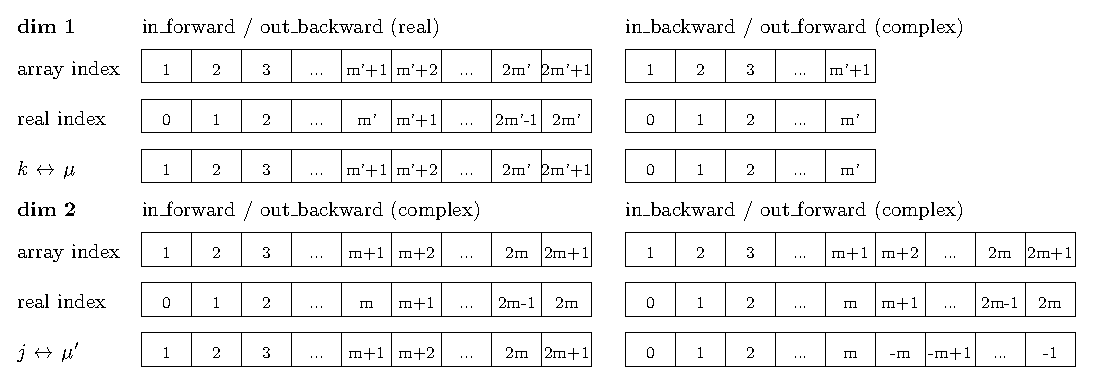
\includegraphics[width=1\textwidth]{_figure/fftw3_indices}
\par\end{center}

\caption[Indices arrangement in a complete forward-backward process of FFT-2D]{Indices arrangement in a complete forward-backward process of FFT-2D.
The DFT of dim 1 ($\Psi_{k}$ to $\mu$) and dim 2 ($\Phi_{k'}$ to
$\mu'$) are done consequentially and \emph{vice versa}. Array index
is the one of Fortran array, real index is the one shown in eq. (\ref{eq:fftw3-fwd})
and (\ref{eq:fftw3-bwd}), $k$ and $k'$ indices shown in the left
as well as $\mu$ and $\mu'$ in the right are those in eq. (\ref{eq:f_mup_mu})
and (\ref{eq:f_mup_mu_2}). Here $\mathrm{m}=m_{\mathrm{max}}$ and
$\mathrm{m}'=\left\lfloor m_{\mathrm{max}}/s\right\rfloor $. \label{fig:FFTW3-2D-indices}}
%
\end{minipage}
\end{figure}


\begin{figure}[h]
\centering{}%
\begin{minipage}[t]{1\textwidth}%
\begin{center}
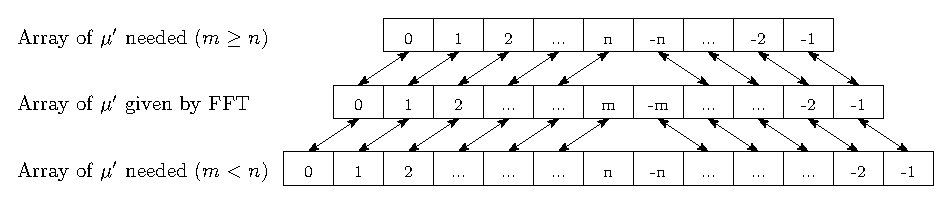
\includegraphics[width=1\textwidth]{_figure/mmax_to_nmax}
\par\end{center}

\caption[mmax to nmax]{mmax to nmax\label{fig:FFTW3-2D-mmax_to_nmax}}
%
\end{minipage}
\end{figure}


As the output array of FFTW3 is periodic
\begin{equation}
e^{2\pi i\mu k/n}=e^{2\pi i(\mu-n)k/n}e^{2\pi ik}=e^{2\pi i(\mu-n)k/n}\label{eq:mu-periodicity}
\end{equation}
the indices $\mu=m_{\mathrm{max}}+1,\ldots,2m_{\mathrm{max}}$ actually
corresponding to $\mu=-m_{\mathrm{max}},\ldots,-1$. It should be
noticed that eq. (\ref{eq:f_mup_mu}) and (\ref{eq:f_mup_mu_2}) don't
possess the periodicity of eq. (\ref{eq:mu-periodicity}), just in
the domain of definition of $\mu'$ and $\mu$ some intermediary functions
share the same formula with FFT.

Moreover, from eq. (\ref{eq:f_mup_mu}), (\ref{eq:f_mup_mu_3}) and
(\ref{eq:symm_f_m_mup_mu}) we can verify that
\begin{equation}
F_{\mu'\mu}(\Theta)=F_{-\mu',-\mu}^{*}(\Theta)
\end{equation}
The later is used in the code because according to the definition
in eq. (\ref{eq:fftw3-fwd}) and (\ref{eq:fftw3-bwd}), $F_{-\mu',-\mu}(\Theta)$
is calculated instead of $F_{\mu'\mu}(\Theta)$.


\section{Operational algorithm\label{sec:Operational-algorithm}}

As described above, the whole process of $\gamma$ and $\mathcal{F}_{\mathrm{exc}}$
functional evaluation is as shown: 

Firstly, the solvent density variable $\Delta\rho(\mathbf{r},\mathbf{\Omega})$
is expended on generalized spherical harmonics
\begin{equation}
\Delta\rho_{\mu'\mu}^{m}(\mathbf{r})=\frac{f_{m}}{8\pi^{2}}\int\mathrm{d}\mathbf{\Omega}\Delta\rho(\mathbf{r},\mathbf{\Omega})R_{\mu'\mu}^{m*}(\mathbf{\Omega})\label{eq:fgsht-fwd}
\end{equation}


Then the Fourier transform of these projections are computed
\begin{equation}
\Delta\hat{\rho}_{\mu'\mu}^{m}(\mathbf{k})=\int\mathrm{d}\mathbf{r}\Delta\rho_{\mu'\mu}^{m}(\mathbf{r})e^{-i\mathbf{r}\cdot\mathbf{k}}\label{eq:fft3d-fwd}
\end{equation}


Then the projections in k-frame are then rotated into local coordinates
system along the unit vector $\mathbf{\hat{k}}$
\begin{equation}
\Delta\hat{\rho'}_{\chi\mu}^{m}(\mathbf{k})=\sum_{\mu'}\Delta\hat{\rho}_{\mu'\mu}^{m}(\mathbf{k})R_{\mu'\chi}^{m}(\mathbf{\hat{k}})
\end{equation}
where the evaluation of rotation matrix elements by recurrence is
detailed \textcolor{red}{in appendix.}

Then computing the OZ equation with Blum's reduction
\begin{equation}
\hat{\gamma'}_{\chi\mu}^{m}(\mathbf{k})=\sum_{n,\nu}(-1)^{\chi+\nu}\hat{c}_{\mu\nu,\chi}^{mn}(\mathbf{k})\Delta\hat{\rho'}_{\chi\underline{\nu}}^{n}(\mathbf{k})\label{eq:OZ-2}
\end{equation}


Then the $\gamma$ projections are then transformed back to global
coordinates system
\begin{equation}
\hat{\gamma}_{\mu'\mu}^{m}(\mathbf{k})=\sum_{\chi}\hat{\gamma'}_{\chi\mu}^{m}(\mathbf{k})R_{\mu'\chi}^{m*}(\mathbf{\hat{k}})
\end{equation}


Then the inverse Fourier transform of these projections
\begin{equation}
\gamma_{\mu'\mu}^{m}(\mathbf{r})=\int\mathrm{d}\mathbf{k}\hat{\gamma}_{\mu'\mu}^{m}(\mathbf{k})e^{i\mathbf{r}\cdot\mathbf{k}}
\end{equation}


Then the function in angular frame can thus be rebuilt
\begin{equation}
\gamma(\mathbf{r},\mathbf{\Omega})=\sum_{m,\mu',\mu}f_{m}\gamma_{\mu'\mu}^{m}(\mathbf{r})R_{\mu'\mu}^{m}(\mathbf{\Omega})\label{eq:fgsht-bwd}
\end{equation}


Finally, the functional $\mathcal{F}_{\mathrm{exc}}$ is computed
by
\begin{equation}
\mathcal{F}_{\mathrm{exc}}=\frac{1}{2}\int\mathrm{d}\mathbf{r}\mathrm{d}\mathbf{\Omega}\Delta\rho(\mathbf{r},\mathbf{\Omega})\gamma(\mathbf{r},\mathbf{\Omega})
\end{equation}



\subsection{Reduction by symmetry\label{sub:Reduction-by-symmetry}}

A further reduction of computing cost can be made by performing approximately
only a half of operations, thanks to the symmetric relations between
the projections.

In eq. (\ref{eq:fgsht-fwd}), $\Delta\rho(\mathbf{r},\mathbf{\Omega})$
is real. Thanks to the property of GSH \textcolor{red}{(eq. (appendix))}
\[
R_{\mu'\mu}^{m}(\mathbf{\Omega})=(-)^{\mu'+\mu}R_{-\mu'-\mu}^{m*}(\mathbf{\Omega})
\]
we find
\begin{equation}
\Delta\hat{\rho}_{\mu'\mu}^{m}(\mathbf{r})=(-)^{\mu'+\mu}\Delta\hat{\rho}_{-\mu',-\mu}^{m*}(\mathbf{r})\label{eq:0}
\end{equation}
therefore only $\mu'>0$ or $\mu>0$ is needed to generate all information.

When $\Delta\hat{\rho}_{\mu'\mu}^{m}(\mathbf{r})$ is transformed
into $k$-space, replace eq. (\ref{eq:0}) into eq. (\ref{eq:fft3d-fwd})
gives
\begin{equation}
\Delta\hat{\rho}_{\mu'\mu}^{m}(\mathbf{k})=(-)^{\mu'+\mu}\Delta\hat{\rho}_{-\mu'-\mu}^{m*}(-\mathbf{k})\label{eq:1}
\end{equation}
thus only the projections of $\mu'>0$, $\mu>0$ or $\mathbf{k}$
where one of the dimensions $k_{i}>0$ are independent.

The rotation to local frame is reigned by the relation \textcolor{red}{(prove?)}
\begin{equation}
R_{\mu'\chi}^{m}(\hat{\mathbf{k}})=(-)^{m}R_{\mu',-\chi}^{m}(-\hat{\mathbf{k}})=(-)^{m+\mu'+\chi}R_{-\mu',\chi}^{m}(-\hat{\mathbf{k}})\label{eq:3}
\end{equation}
which gives
\begin{equation}
\Delta\hat{\rho'}_{\chi\mu}^{m}(\mathbf{k})=(-)^{m+\mu+\chi}\Delta\hat{\rho'}_{\chi,-\mu}^{m*}(-\mathbf{k})\label{eq:2}
\end{equation}
Thanks to the symmetry\textcolor{red}{{} (eq. (appendix))} 
\begin{equation}
\hat{c'}_{\mu\nu,\chi}^{mn}(k)=(-)^{m+n+\mu+\nu}\hat{c'}_{\underline{\mu}\underline{\nu},\chi}^{mn*}(k)
\end{equation}
\begin{equation}
\hat{c'}_{\mu\nu,\chi}^{mn}(k)=(-)^{m+n}\hat{c'}_{\nu\mu,\chi}^{nm}(k)
\end{equation}
\begin{equation}
\hat{c'}_{\mu\nu,\underline{\chi}}^{mn}(k)=\hat{c'}_{\underline{\mu}\underline{\nu},\chi}^{mn}(k)=(-)^{m+n}\hat{c'}_{\mu\nu,\chi}^{mn*}(k)
\end{equation}
$\hat{\gamma'}_{\chi\mu}^{m}(\mathbf{k})$ possesses the same symmetry.
Thus OZ equation can be reduced by a factor two.

\begin{figure}[h]
\begin{centering}
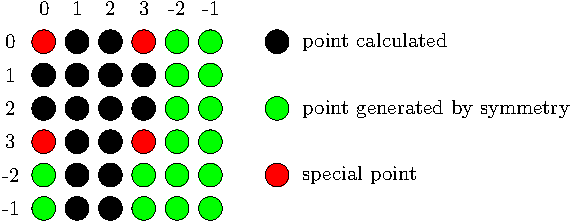
\includegraphics{_figure/test_lmn}
\par\end{centering}

\caption{Distribution of points to be calculated according to symmetry in a
2D plan}
\end{figure}



\subsection{Commutativity between operations\label{sub:Commutativity-between-operations}}

As mentioned in the operational algorithm, three types of operation
are being done before and after OZ equation. They are
\begin{enumerate}
\item Fast Fourier transform for 3-dimensional spatial grid (FFT3D): implemented
by package FFTW3 \citep{FFTW3}, mathematically leading to no accuracy
lost.
\item Fast generalized spherical harmonics transform (FGSHT): have real
or complex input, is exact if $F(\mathbf{\Omega})$ is a polynomial
of $\cos\Theta$, $\cos\Phi$ and $\cos\Psi$ of order at most $m_{\mathrm{max}}$.
\item Rotation between laboratory coordinate system and local system linked
to vector $\mathbf{k}$ (RotS): can be done for both function and
projections. It introduces a minus error in accuracy at origin and
border of the box, it will be discussed in next chapter.
\end{enumerate}
Their commutativity is shown in figure \ref{fig:Commutativity-of-operations}.

\begin{figure}[h]
\begin{centering}
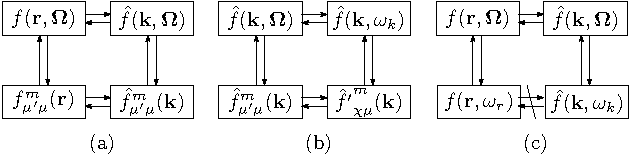
\includegraphics{_figure/algorithms_commutativity}
\par\end{centering}

\caption[Commutativity of operations]{Commutativity of operations. (a) FFT3D and FGSHT; (b) RotS and FGSHT;
(c) FFT3D and RotS\label{fig:Commutativity-of-operations}}
\end{figure}



\subsubsection{FFT3D and FGSHT}

The FFT3D

\[
f(\mathbf{r})=\int\hat{f}(\mathbf{k})e^{i\mathbf{k}\cdot\mathbf{r}}
\]
\[
\hat{f}(\mathbf{k})=\int f(\mathbf{r})e^{-i\mathbf{k}\cdot\mathbf{r}}
\]
does not depend on the angular part of function, and
\[
f(\mathbf{\Omega})=\sum_{m\mu'\mu}f_{m}f_{\mu'\mu}^{m}R_{\mu'\mu}^{m}(\mathbf{\Omega})
\]
\[
f_{\mu'\mu}^{m}=\int f_{m}f(\mathbf{\Omega})R_{\mu'\mu}^{m}(\mathbf{\Omega})
\]
does not depend on the spatial part of function. The two operations
are commutative.


\subsubsection{FGSHT and coordinate rotation}

Function $\hat{f'}$ intermolecular frame can be deduced from the
function $\hat{f}$ in laboratory frame 
\[
\hat{f}(\mathbf{k},\mathbf{\Omega})=\hat{f'}(\mathbf{k},\boldsymbol{\omega}_{k})
\]
where the two can both be expended on GSH

\[
\hat{f}(\mathbf{k},\mathbf{\Omega})=\sum_{m\mu'\mu}f_{m}\hat{f}_{\mu'\mu}^{m}(\mathbf{k})R_{\mu'\mu}^{m}(\mathbf{\Omega})
\]


\[
\hat{f'}(\mathbf{k},\boldsymbol{\omega}_{k})=\sum_{m\chi\mu}f_{m}\hat{f'}_{\chi\mu}^{m}(\mathbf{k})R_{\chi\mu}^{m}(\boldsymbol{\omega}_{k})
\]


And the relation between projections are simple

\[
f'{}_{\chi\mu}^{m}(\mathbf{k})=\sum_{\mu'}R_{\mu'\chi}^{m}(\hat{\mathbf{k}})f_{\mu'\mu}^{m}(\mathbf{k})
\]
\[
f_{\mu'\mu}^{m}(\mathbf{k})=\sum_{\chi}R_{\mu'\chi}^{m*}(\hat{\mathbf{k}})f'{}_{\chi\mu}^{m}(\mathbf{k})
\]
The two operations are commutative.


\subsubsection{Coordinate rotation and FFT3D}

The rotation from $f(\mathbf{r},\mathbf{\Omega})$ to $f(\mathbf{r},\boldsymbol{\omega})$
depends on the vector $\mathbf{r}$, of which the information is totally
lost after FFT3D. The rotation from $f(\mathbf{k},\mathbf{\Omega})$
to $f(\mathbf{k},\boldsymbol{\omega})$ can only depend on the vector
$\mathbf{k}$, they are not the same rotation. Non-commutative. 



\chapter{Free Energy and Related Thermodynamic Quantities\label{chpt:thermodynamic-quantities}}

The solvation free energy is the most important property that we seek;
as shown in previous sections, it can be calculated by the minimization
of free energy functional $\mathcal{F}[\rho]$. Here is a discussion
about some corrections needed for charged solutes and some related
thermodynamic quantities that can be obtained directly from the solvation
free energy.

The solvation properties often involve the three-dimensional microscopic
structure of the solvent around the dissolved molecule, as well as
thermodynamic quantities such as the enthalpy, entropy, and free
energy of solvation {[}ref gubbins{]} pKa {[}ref{]}.

The solvation properties can be determined if the two principle properties, free energy and structure,
are accurately calculated. In this thesis,
we focus on these two aspects.


\section{Free energy correction for a single ion}

In the calculation of external potential as well as the total solvation
free energy, the use of different conventions can lead to a charge-independent
offset, which introduces error for charged solutes \citep{Kastenholz_2006_I,Kastenholz_2006_II,Hunenberger_book}.
This offset is mainly caused by two sources: (1) resulting from the use of
a finite system size; in our case, a system with cubic periodic
boundary conditions, which presents artificial interactions between
the ion and its own periodic copies, as well as between the solvent
and the periodic copies of the ion (Type-B in \citep{Kastenholz_2006_II});
(2) owing to the choice of convention for summing up the contributions
of solvent charges to the electrostatic potential in the sample system
(Type-C in \citep{Kastenholz_2006_II}).


\subsection{Correction of type B}

Type B correction should be added for systems with finite size or
periodic boundary conditions, accounting for the error in the solvent
polarization \marginpar{Another way to evaluate this error is to make a numerical extrapolation
of the inverse of the box size $\left(1/L\right)$; it is more accurate
but demands much more calculation.}
\begin{equation}
\Delta G_{B}=\frac{1}{8\pi\varepsilon_{0}}\left(1-\varepsilon^{-1}\right)\frac{q^{2}}{L}\left[\xi+\frac{4\pi}{3}\left(\frac{R_{\mathrm{I}}}{L}\right)^{2}-\frac{16\pi}{45}\left(\frac{R_{\mathrm{I}}}{L}\right)^{5}\right]\label{eq:corr-B}
\end{equation}
where

\begin{tabular}{cl}
 $\varepsilon_{0}$ & is the vacuum permittivity;\tabularnewline
$\varepsilon$ is the solvent permittivity (dielectric constant);\tabularnewline
$q$ & is the solute charge;\tabularnewline
$L$ & \textcolor{red}{is the box length};\tabularnewline
$R_{\mathrm{I}}$ & is the ionic radius;\tabularnewline
$\xi$ & \textcolor{red}{is the energy per particle in a simple cubic lattice,}
$\xi\simeq-2.837297$ \citep{nijboer}.\tabularnewline
 & \tabularnewline
\end{tabular} 

As $R_{\mathrm{I}}$ is significantly smaller than the size of the
computational box, i. e. $R_{\mathrm{I}}\ll L$, its quadratic as
well as higher order of $\left(R_{\mathrm{I}}/L\right)$ is considered
negligible, thus eq. (\ref{eq:corr-B}) becomes
\begin{equation}
\Delta G_{\mathrm{B}}=\frac{\xi}{8\pi\varepsilon_{0}}\left(1-\varepsilon^{-1}\right)\frac{q^{2}}{L}
\end{equation}
\textcolor{red}{It links to Born correction}.


\subsection{Correction of type C}

Type-C corrections are needed when the systems to be compared use different
electrostatic summation schemes: on the basis of point charges within
entire solvent molecules (M scheme) or on the basis of individual
point charges (P scheme), shown in figure \ref{fig:IQ-model-som-scheme}
(c) and (d), which brings a fixed free energy difference at the boundary.

\begin{figure}[h]
\begin{centering}
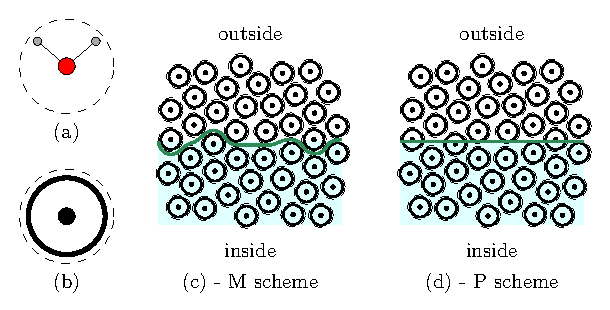
\includegraphics{_figure/ion_correction}
\par\end{centering}

\caption [IQ model and summation scheme]{IQ model and summation scheme. (a) The solvent molecule. (b) The
equivalent isotropic quadrupole (IQ) fluid model. (c) In the M scheme,
one evaluates the Coulombic potential generated by the solvent charges
belonging to all molecules within the boundary. (d) In the P scheme,
one evaluates the Coulombic potential generated by all solvent charges
within the boundary.\label{fig:IQ-model-som-scheme}}
\end{figure}


It can be deduced analytically by considering the solvent as a \textcolor{red}{canonical
ensemble} under the orientational disorder limit (ODL) \citep{Kastenholz_2006_I},
which becomes an isotropic quadrupole (IQ) fluid, whose solvent molecule
(figure \ref{fig:IQ-model-som-scheme} (b)) possesses the same quadrupole
trace $\gamma$ \marginpar{$\gamma$ which is elsewhere referred to as the spheropole moment \citep{Saunders_1992,Maschio_2012},
that is, the spherical component of the quadrupole moment, and is
invariant with respect to rotations.}
\begin{equation}
\gamma=\mathrm{tr}(\mathbf{\mathcal{Q}})=\mathcal{Q}_{xx}+\mathcal{Q}_{yy}+\mathcal{Q}_{zz}
\end{equation}
where the quadrupole moment of the solvent molecule can be calculated
by its definition \citep{Multipole}:
\begin{equation}
\mathcal{Q}_{ij}=\int_{V}r_{i}r_{j}\rho(\mathbf{r})\mathrm{d}v=\sum_{\alpha=1}^{N}q^{(\alpha)}r_{i}^{(\alpha)}r_{j}^{(\alpha)}
\end{equation}


It can be shown that the charge density of a solvent located within the
boundary of a sample system vanishes everywhere except at the boundary
in the M scheme, which results in a uniform normal surface polarization.
The correction needed for\textcolor{red}{{} M scheme }is
\begin{equation}
\Delta G_{\mathrm{C}}=-q\left(1-\frac{4\pi R_{\mathrm{I}}^{3}}{3L^{3}}\right)\Delta\Phi_{\mathrm{ODL}}\label{eq:corr-C}
\end{equation}
where $\Delta\Phi_{\mathrm{ODL}}=\left(6\varepsilon_{0}\right)^{-1}\eta\gamma$,
$\eta$ being the solvent number density.

In the same way, when we consider $R_{\mathrm{I}}\ll L$, eq. (\ref{eq:corr-C})
becomes
\begin{equation}
\Delta G_{\mathrm{C}}=-\left(6\varepsilon_{0}\right)^{-1}\eta\gamma q
\end{equation}



\section{Some related thermodynamic quantities}

Thermodynamic quantities such as the internal energy, pressure, compressibility
and heat capacity are obtained as derivatives of the classical partition
function. {[}Evans poly{]}

Structure and Thermodynamic Properties of Bulk Liquids

Pressure is (virial pressure equation) 
\begin{equation}
p=\rho k_{\mathrm{B}}T-\dfrac{\rho^{2}}{2}\int\mathrm{d}\mathbf{r}g(r)\frac{r}{3}\frac{\mathrm{d}u(r)}{\mathrm{d}r}
\end{equation}


The Gibbs free energy G is simply {[}Evans 1979{]}.

$G=\mu\int\mathrm{d}\mathbf{r}\rho(\mathbf{r})$


\subsection{Solubility}


\subsection{Pressure}

enthalpy, entropy {[}3{]} pH



\chapter{Solvation Structure\label{chpt:solvation-structure}}

In MDFT, all the information about solvation structure can be deduced
from the solvent density $\rho(\mathbf{r},\mathbf{\Omega})$. This
section presents some examples of structure which are used in later
chapters.


\section{Radial distribution function and site-site distribution function}

Radial distribution function (\acs{RDF}) and site-site distribution
function

It should be the same with 


\section{Radial polarization functions}

It should be the same with 


\section{Rotational invariant expansion}

appendix \ref{chpt:rotational-invariant-expansion}


\section{Rebuilt of density in a certain orientation}

appendix \ref{chpt:rotational-invariant-expansion}


\subsection{Radical distribution function of numeric density}

Content.


\subsection{Radical distribution function of polarization}

\[
F(\mathbf{r},\mathbf{\Omega})=\sum_{nl\nu}F_{0\nu}^{0nl}(r)\Phi_{0\nu}^{0nl}(\mathbf{r},\mathbf{\Omega})
\]


conversely

\[
F_{0\nu}^{0nl}(r)=\int\mathrm{d}\hat{\mathbf{r}}\mathrm{d}\mathbf{\Omega}F(\mathbf{r},\mathbf{\Omega})\Phi_{0\nu}^{0nl*}(\mathbf{r},\mathbf{\Omega})/\int\mathrm{d}\hat{\mathbf{r}}\mathrm{d}\mathbf{\Omega}\left\Vert \Phi_{0\nu}^{0nl}(\mathbf{r},\mathbf{\Omega})\right\Vert ^{2}
\]
with

\[
\Phi_{0\nu}^{0nl}(\mathbf{r},\mathbf{\Omega})=f_{n}\sum_{\nu'}\left(\begin{array}{ccc}
0 & n & l\\
0 & \nu' & -\nu'
\end{array}\right)R_{\nu'\nu}^{n}(\mathbf{\Omega})R_{-\nu',0}^{l}(\mathbf{\hat{r}})
\]


in particular

\begin{eqnarray*}
\Phi_{00}^{011}(\mathbf{r},\mathbf{\Omega}) & = & \sqrt{3}\left(\begin{array}{ccc}
0 & 1 & 1\\
0 & 0 & 0
\end{array}\right)R_{00}^{1}(\mathbf{\Omega})R_{00}^{1}(\mathbf{\hat{r}})\\
 & + & \sqrt{3}\left(\begin{array}{ccc}
0 & 1 & 1\\
0 & 1 & -1
\end{array}\right)R_{10}^{1}(\mathbf{\Omega})R_{-10}^{1}(\mathbf{\hat{r}})\\
 & + & \sqrt{3}\left(\begin{array}{ccc}
0 & 1 & 1\\
0 & -1 & 1
\end{array}\right)R_{-10}^{1}(\mathbf{\Omega})R_{10}^{1}(\mathbf{\hat{r}})
\end{eqnarray*}
or
\begin{eqnarray*}
\Phi_{00}^{011}(\mathbf{r},\mathbf{\Omega}) & = & -3R_{00}^{1}(\mathbf{\Omega})R_{00}^{1}(\mathbf{\hat{r}})\\
 & + & 3R_{10}^{1}(\mathbf{\Omega})R_{-10}^{1}(\mathbf{\hat{r}})\\
 & + & 3R_{-10}^{1}(\mathbf{\Omega})R_{10}^{1}(\mathbf{\hat{r}})
\end{eqnarray*}
noting 

\[
R_{00}^{1}(\mathbf{\Omega})=\cos\theta
\]


\[
R_{10}^{1}(\mathbf{\Omega})=-\frac{1}{\sqrt{2}}\sin\theta e^{-i\phi}
\]


one finds
\begin{eqnarray*}
\Phi_{00}^{011}(\mathbf{r},\mathbf{\Omega}) & = & -3R_{00}^{1}(\mathbf{\Omega})R_{00}^{1}(\mathbf{\hat{r}})\\
 & + & 3R_{10}^{1}(\mathbf{\Omega})R_{-10}^{1}(\mathbf{\hat{r}})\\
 & + & 3R_{-10}^{1}(\mathbf{\Omega})R_{10}^{1}(\mathbf{\hat{r}})\\
 & = & -3\mathbf{\Omega}\cdot\hat{\mathbf{r}}
\end{eqnarray*}


such that

\begin{eqnarray*}
F_{00}^{011}(r) & = & -\frac{1}{3}\int\\
 & = & P(\mathbf{r})\cdot\hat{\mathbf{r}}\\
\end{eqnarray*}


proportionality coefficient to be determined precisely... One thus
gets the radial projection of the polarization.

Content.


\ctparttext{The code MDFT developed in this thesis is based on the branch master
of Git project MDFT (\url{https://github.com/maxlevesque/MDFT/}),
version {[}Fri Jun 20 19:05:52 2014 +0200{]}. All the implementations
are run on \textsf{\textbf{POINCARE}} machines of IDRIS, which involved
two kinds of machines:\\
\medskip{}
\textsf{\textbf{poincare{[}001-092{]}:}} 2 processors Sandy Bridge
E5-2670 (2.60GHz, 8 cores per processor, being 16 cores per node);
32 GB of memory per node.\\
\medskip{}
\textsf{\textbf{poincarebig{[}01-02{]}:}} 4 processors AMD Opteron
6282 (2.60GHz, 16 cores per processor, being 64 cores per node); 128
GB of memory per node.\\
\medskip{}
The former is used for regular calculation, whose memory hierarchy
is shown in figure \ref{fig:poincare}. The later is only used in
the evaluation of accuracy, in case of memory leak in the former.\\
\medskip{}
\begin{figure}[h]
\begin{centering}
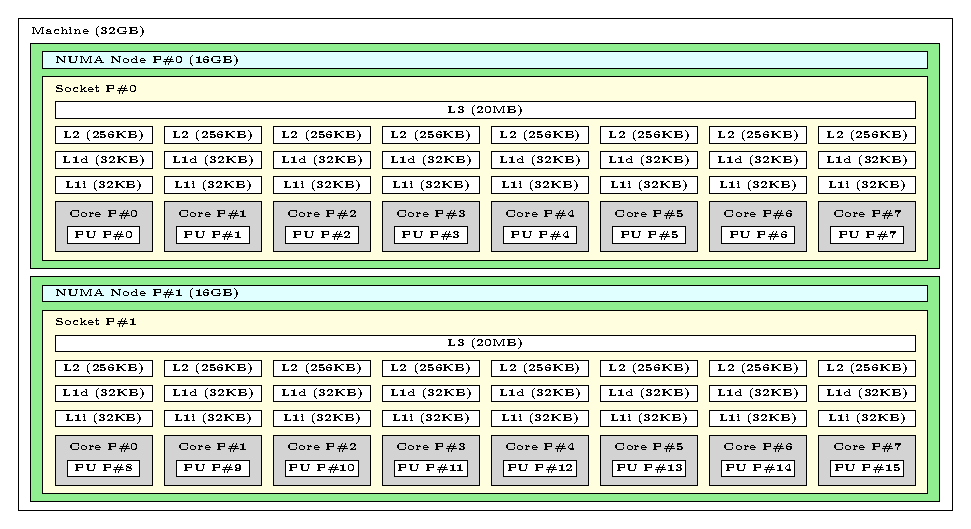
\includegraphics[width=0.9\columnwidth]{_figure/poincare}
\par\end{centering}
\caption{Structure of a POINCARE node\label{fig:poincare}}
\end{figure}
\medskip{}
Section \ref{chpt:algorithms-and-branches},\\
\medskip{}
Section \ref{chpt:accuracy} discussion on precision,\\
\medskip{}
Section \ref{chpt:seq-code-performance} computing performance and
memory limits,\\
\medskip{}
Section \ref{chpt:parallelization} OpenMP, MPI giving the possibility
to go beyond the memory limit. Due to the complexity of minimizer
L-BFGS, this process is only added on the part of $\mathcal{F}_{\mathrm{exc}}$
evaluation. Tests of performance stability with respect to both threads
and nodes are made.}

\part{Implementation}


\chapter{Algorithms and Branches\label{chpt:algorithms-and-branches}}

According to the commutativity of operations (see $\mathsection$\ref{subsec:Commutativity-between-operations}),
the only possible algorithms to evaluate $\gamma(\mathbf{r},\mathbf{\Omega})$
from $\Delta\rho(\mathbf{r},\mathbf{\Omega})$ are shown in the figure
\ref{fig:Possible-algorithms}.

\begin{figure}[h]
\begin{centering}
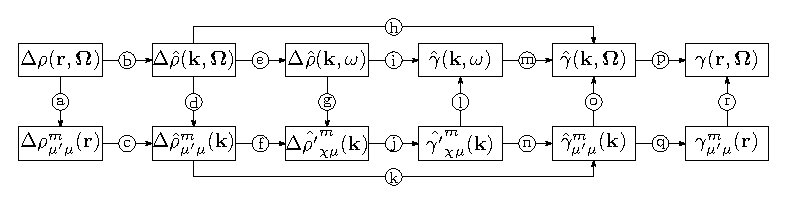
\includegraphics{_figure/algorithms}
\par\end{centering}
\caption{Possible algorithms for $\gamma$ evaluation\label{fig:Possible-algorithms}}
\end{figure}

Several branches are built to test and compare between algorithms,
which are shown below in table \ref{tab:Branch-option} and will be
detailed in the following context. \marginpar{These branches should give numerically the same result in certain
conditions, that will be discussed in later sections.}

\selectlanguage{english}%
\begin{table}[h]
\selectlanguage{american}%
\begin{centering}
\begin{tabular*}{1\textwidth}{@{\extracolsep{\fill}}cccc}
\toprule 
\tableheadline{Method} & \tableheadline{Sub-Method} & \tableheadline{Description} & \tableheadline{Theory}\tabularnewline
\midrule
reference & dipole & calculate $n(r)$ and $P(r)$ separately & $\mathsection$\ref{chpt:mdft} \textcolor{red}{{[}ref{]}}\tabularnewline
\midrule
naive & standard & use $c_{\mu\nu,\chi}^{mn}(k)$ as input DCF & $\mathsection$\ref{subsec:Using-projections-in-1}\tabularnewline
 & zero-order & use $\hat{c}(k,\boldsymbol{\omega_{1}},\boldsymbol{\omega_{2}})$
and take the nearest point & $\mathsection$\ref{subsec:Zero-order-interpolation-of}\tabularnewline
 & interpolation & use $\hat{c}(k,\boldsymbol{\omega_{1}},\boldsymbol{\omega_{2}})$
with linear interpolation  & $\mathsection$\ref{subsec:Linear-interpolation-of}\tabularnewline
 & dipole & use $c_{S}$, $c_{\Delta}$, $c_{D}$ issue from \textcolor{red}{{[}ref{]}} & $\mathsection$\ref{subsec:Using-projections-in}\tabularnewline
 & nmax1 & use $c_{S}$, $c_{\Delta}$, $c_{D}$, $c_{\pm}$ issue from \textcolor{red}{{[}ref{]}} & $\mathsection$\ref{subsec:Using-projections-in}\tabularnewline
\midrule
convolution & standard & algorithm with symmetry reduction & $\mathsection$\ref{subsec:Reduction-by-symmetry}\tabularnewline
 & asymm  & algorithm without symmetry reduction & $\mathsection$\ref{subsec:Reduction-by-symmetry}\tabularnewline
 & pure\_angular  & inverse FFT and FGSHT & $\mathsection$\ref{chpt:algorithms-and-branches}\tabularnewline
\bottomrule
\end{tabular*}
\par\end{centering}
\selectlanguage{english}%
\caption{\foreignlanguage{american}{Branch option in MDFT\label{tab:Branch-option}}}
\end{table}

\selectlanguage{american}%

\section{Branches \textquotedbl{}naive\textquotedbl{} }

Branches \texttt{\textbf{naive}} are the algorithms mentioned in section
\ref{chpt:fft-spatial}, which go through the path 
\[
\left(b\right)\shortrightarrow\left(h\right)\shortrightarrow\left(p\right)
\]
 in figure \ref{fig:Possible-algorithms}, calculating directly $\hat{\gamma}(\mathbf{k},\mathbf{\Omega})$
from $\Delta\hat{\rho}(\mathbf{k},\mathbf{\Omega})$. The difference
between branches is the way to calculate $\hat{c}(\mathbf{k},\mathbf{\Omega_{1}},\mathbf{\Omega_{2}})$.
Branch\textbf{ }\texttt{\textbf{naive\_standard}} use $c_{\mu\nu,\chi}^{mn}(k)$
as input \acs{DCF}. Branch \texttt{\textbf{naive\_zero-order}} and
\texttt{\textbf{naive\_interpolation}} using $\hat{c}(k,\boldsymbol{\omega_{1}},\boldsymbol{\omega_{2}})$
with zero-order and linear interpolation, where the former is rejected
in the implementation due to a lack of precision (appendix \ref{chpt:error-evaluation-interpolation-DCF}).

\section{Branches \textquotedbl{}convolution\textquotedbl{}}

Branches\textbf{ }\texttt{\textbf{convolution\_asymm}} and \texttt{\textbf{convolution\_standard}}
are operational algorithms of angular convolution show in section
\ref{chpt:angular-convolution}, which go through the path 
\[
\left(a\right)\shortrightarrow\left(c\right)\shortrightarrow\left(f\right)\shortrightarrow\left(j\right)\shortrightarrow\left(n\right)\shortrightarrow\left(q\right)\shortrightarrow\left(r\right)
\]

Branches\textbf{ }\texttt{\textbf{convolution\_asymm}} uses the original
operational algorithm ($\mathsection$\ref{sec:Operational-algorithm})
without symmetry reduction ($\mathsection$\ref{subsec:Reduction-by-symmetry}),
and \texttt{\textbf{convolution\_standard}} with it. 

Branch \texttt{\textbf{convolution\_pure\_angular}} goes through the
path 
\[
\left(b\right)\shortrightarrow\left(d\right)\shortrightarrow\left(f\right)\shortrightarrow\left(j\right)\shortrightarrow\left(n\right)\shortrightarrow\left(o\right)\shortrightarrow\left(p\right)
\]
which inverse the first and last two steps of the two algorithms mentioned
above.

\section{Testing branches for $n_{\max}$=1}

Branches \texttt{\textbf{naive\_dipole}}, \texttt{\textbf{naive\_nmax1}}
pass by $\left(b\right)\shortrightarrow\left(h\right)\shortrightarrow\left(p\right)$
, using DCF separately of the references \textcolor{red}{{[}ref{]}}
and \textcolor{red}{{[}ref{]}}, whose slight difference is shown in
$\mathsection$\ref{subsec:Comparison-with-non-coupling}. Branch
\texttt{\textbf{reference\_dipole}} use DCF in \textcolor{red}{{[}ref{]}},
which is the original method in MDFT to calculate $\mathcal{F}_{\mathrm{exc}}$
via multipole expansion. In addition with branch \texttt{\textbf{convolution\_standard}},
which can also use the two DCF mentioned above, a test of validation
can be performed, which should at any case exactly numerically the
same if the same DCF is used.

\section{Other paths}

Considering the necessity, other paths such as those passing by $\left(i\right)$
and $\left(k\right)$ are only built for local test usage (c. f. discussion
in following sections).



\chapter{Numerical and Physical Accuracy\label{chpt:accuracy}}

This chapter gives a systematic comparison between algorithms for
the evaluation of the excess free energy $\mathcal{F}_{\mathrm{exc}}$
and its gradient $\gamma$ in terms of accuracy. As the theory does
not contain any unpredictable random part, the comportment of the
code is mathematically predictable. For example, certain algorithms
should give the same result at machine precision ($10^{-13}$ to $10^{-15}$)
in certain conditions. A loss of accuracy comparing to the prediction
can be classified as two different types. One is the theoretical loss;
for instance, a certain equation is only valid for an infinite order.
This kind of loss is unavoidable but should be worked out explicitly.
Another source is the unknown loss, containing all kinds of incompatibility
in the result that cannot be explained mathematically. It is mainly attributable to a bug in the implementation that cannot be located. There is also the possibility that it is a theoretical loss which has not been worked out. All these comparisons aim to give a global view of the credibility for the results given by this code.

\section{Generalized spherical harmonics transform\label{sec:gsh-imp}}

As discussed in $\mathsection$\ref{sec:fgsht}, the function after
a forward-backward \acs{GSHT} process 
\begin{equation}
F_{\mu'\mu}^{m}=\frac{f_{m}}{8\pi^{2}}\sum_{i=0}^{m_{\mathrm{max}}}w_{i}\sum_{j=0}^{2m_{\mathrm{max}}}\sum_{k=0}^{2\left\lfloor m_{\mathrm{max}}/s\right\rfloor }F(\Theta_{i},\Phi_{j},\Psi_{k})R_{\mu'\mu}^{m*}(\Theta_{i},\Phi_{j},\Psi_{k})
\end{equation}
\begin{equation}
F(\Theta_{i},\Phi_{j},\Psi_{k})=\sum_{m=0}^{n_{\mathrm{max}}}f_{m}\sum_{\mu'=-m}^{m}\sum_{\underset{\mod(\mu,s)=0}{\mu=-m}}^{m}F_{\mu'\mu}^{m}R_{\mu'\mu}^{m}(\Theta_{i},\Phi_{j},\Psi_{k})
\end{equation}
only remains the same when it is a polynomial of both $\cos\Theta$,
$\cos\Phi$ and $\cos\Psi$ of order $n_{\max}$, where $n_{\max}$
is the highest order of \acs{GSH} in the expansion, and $m_{\max}=n_{\max}$
the order of quadrature used. However, as in reality, the density
variable $\rho$ is not a simple polynomial, and the choice of $m_{\max}$
and $n_{\max}$ is tightly linked to the performance. It is important
to know how much these choices will affect the results. The \acs{FFT}
process is implemented by package FFTW3 \citep{FFTW3}, which is verified
to be leading to strictly no accuracy lost (at machine precision).
That means the \acs{FGSHT} process will have strictly with the \acs{GSHT} %'will have strictly'? Something is missing.
process. Here we do not need to distinguish the two.

\subsection{$m_{\mathrm{max}}$ and $n_{\mathrm{max}}$ of projections}

The numerical error tests of a forward-backward GSHT process with
different order $n_{\mathrm{max}}$ of GSH and $m_{\mathrm{max}}$
of quadrature are shown in table \ref{tab:error-gsh}.
\begin{table}[H]
\begin{centering}
\subfloat[$f(\mathbf{\Omega})=1$]{\begin{centering}
\begin{tabular*}{1\columnwidth}{@{\extracolsep{\fill}}ccccccc}
\toprule 
{\footnotesize{}$m$\textbackslash{}$n$} & \multirow{1}{*}{{\footnotesize{}0}} & \multirow{1}{*}{{\footnotesize{}1}} & {\footnotesize{}2} & \multirow{1}{*}{{\footnotesize{}3}} & \multirow{1}{*}{{\footnotesize{}4}} & \multirow{1}{*}{{\footnotesize{}5}}\tabularnewline
\midrule
\multicolumn{1}{c}{{\footnotesize{}0}} & \textbf{\footnotesize{}0 (0)} & {\footnotesize{}9.00 (3.00)} & {\footnotesize{}34.00 (18.00)} & {\footnotesize{}83.00 (39.00)} & {\footnotesize{}164.00 (84.00)} & {\footnotesize{}285.00 (139.00)}\tabularnewline
\multicolumn{1}{c}{{\footnotesize{}1}} & \textbf{\footnotesize{}0 (0)} & \textbf{\footnotesize{}0 (0)} & {\footnotesize{}0 (1.67)} & {\footnotesize{}4.34 (6.07)} & {\footnotesize{}7.06 (13.63)} & {\footnotesize{}14.88 (17.30)}\tabularnewline
\multicolumn{1}{c}{{\footnotesize{}2}} & \textbf{\footnotesize{}0 (0)} & \textbf{\footnotesize{}0 (0)} & \textbf{\footnotesize{}0 (0)} & {\footnotesize{}0 (0)} & {\footnotesize{}0 (0)} & {\footnotesize{}5.65 (2.71)}\tabularnewline
{\footnotesize{}3} & \textbf{\footnotesize{}0 (0)} & \textbf{\footnotesize{}0 (0)} & \textbf{\footnotesize{}0 (0)} & \textbf{\footnotesize{}0 (0)} & {\footnotesize{}0 (0)} & {\footnotesize{}0 (0)}\tabularnewline
\multicolumn{1}{c}{{\footnotesize{}4}} & \textbf{\footnotesize{}0 (0)} & \textbf{\footnotesize{}0 (0)} & \textbf{\footnotesize{}0 (0)} & \textbf{\footnotesize{}0 (0)} & \textbf{\footnotesize{}0 (0)} & {\footnotesize{}0 (0)}\tabularnewline
\multicolumn{1}{c}{{\footnotesize{}5}} & \textbf{\footnotesize{}0 (0)} & \textbf{\footnotesize{}0 (0)} & \textbf{\footnotesize{}0 (0)} & \textbf{\footnotesize{}0 (0)} & \textbf{\footnotesize{}0 (0)} & \textbf{\footnotesize{}0 (0)}\tabularnewline
\bottomrule
\end{tabular*}
\par\end{centering}
}
\par\end{centering}
\begin{centering}
\subfloat[$f(\mathbf{\Omega})=\cos3\Theta$]{\begin{centering}
\begin{tabular*}{1\columnwidth}{@{\extracolsep{\fill}}ccccccc}
\toprule 
{\footnotesize{}$m$\textbackslash{}$n$} & \multirow{1}{*}{{\footnotesize{}0}} & \multirow{1}{*}{{\footnotesize{}1}} & {\footnotesize{}2} & \multirow{1}{*}{{\footnotesize{}3}} & \multirow{1}{*}{{\footnotesize{}4}} & \multirow{1}{*}{{\footnotesize{}5}}\tabularnewline
\midrule
\multicolumn{1}{c}{{\footnotesize{}0}} & {\footnotesize{}0 (0)} & {\footnotesize{}0 (0)} & {\footnotesize{}0 (0)} & {\footnotesize{}0 (0)} & {\footnotesize{}0 (0)} & {\footnotesize{}0 (0)}\tabularnewline
\multicolumn{1}{c}{{\footnotesize{}1}} & {\footnotesize{}0.96 (0.96)} & {\footnotesize{}0 (0)} & {\footnotesize{}0 (0)} & {\footnotesize{}2.56 (6.99)} & {\footnotesize{}10.76 (14.15)} & {\footnotesize{}13.83 (21.21)}\tabularnewline
\multicolumn{1}{c}{{\footnotesize{}2}} & {\footnotesize{}0.46 (0.46)} & {\footnotesize{}0 (0)} & {\footnotesize{}0 (0)} & {\footnotesize{}0 (0)} & {\footnotesize{}0 (0)} & {\footnotesize{}1.36 (0.50)}\tabularnewline
{\footnotesize{}3} & {\footnotesize{}0.86 (0.86)} & {\footnotesize{}0.66 (0.66)} & {\footnotesize{}0.66 (0.66)} & \textbf{\footnotesize{}0 (0)} & {\footnotesize{}0 (0)} & {\footnotesize{}0.66 (0.66)}\tabularnewline
\multicolumn{1}{c}{{\footnotesize{}4}} & {\footnotesize{}0.99 (0.99)} & {\footnotesize{}0.80 (0.80)} & {\footnotesize{}0.80 (0.80)} & \textbf{\footnotesize{}0 (0)} & \textbf{\footnotesize{}0 (0)} & {\footnotesize{}0 (0)}\tabularnewline
\multicolumn{1}{c}{{\footnotesize{}5}} & {\footnotesize{}0.83 (0.83)} & {\footnotesize{}1.01 (1.01)} & {\footnotesize{}1.01 (1.01)} & \textbf{\footnotesize{}0 (0)} & \textbf{\footnotesize{}0 (0)} & \textbf{\footnotesize{}0 (0)}\tabularnewline
\bottomrule
\end{tabular*}
\par\end{centering}
}
\par\end{centering}
\begin{centering}
\subfloat[$f(\mathbf{\Omega})=\cos3\Phi$]{\begin{centering}
\begin{tabular*}{1\columnwidth}{@{\extracolsep{\fill}}ccccccc}
\toprule 
{\footnotesize{}$m$\textbackslash{}$n$} & \multirow{1}{*}{{\footnotesize{}0}} & \multirow{1}{*}{{\footnotesize{}1}} & {\footnotesize{}2} & \multirow{1}{*}{{\footnotesize{}3}} & \multirow{1}{*}{{\footnotesize{}4}} & \multirow{1}{*}{{\footnotesize{}5}}\tabularnewline
\midrule
\multicolumn{1}{c}{{\footnotesize{}0}} & {\footnotesize{}0 (0)} & {\footnotesize{}9.00 (3.00)} & {\footnotesize{}34.00 (18.00)} & {\footnotesize{}83.00 (39.00)} & {\footnotesize{}164.00 (84.00)} & {\footnotesize{}285.00 (139.00)}\tabularnewline
\multicolumn{1}{c}{{\footnotesize{}1}} & {\footnotesize{}0 (0)} & {\footnotesize{}0 (0)} & {\footnotesize{}0 (1.67)} & {\footnotesize{}4.34 (6.07)} & {\footnotesize{}7.06 (13.63)} & {\footnotesize{}14.88 (17.30)}\tabularnewline
\multicolumn{1}{c}{{\footnotesize{}2}} & {\footnotesize{}1.00 (1.00)} & {\footnotesize{}1.00 (1.00)} & {\footnotesize{}0.50 (0.50)} & {\footnotesize{}1.53 (1.53)} & {\footnotesize{}1.15 (1.15)} & {\footnotesize{}3.65 (0.89)}\tabularnewline
{\footnotesize{}3} & {\footnotesize{}1.00 (1.00)} & {\footnotesize{}1.00 (1.00)} & {\footnotesize{}1.00 (1.00)} & {\footnotesize{}0.83 (0.83)} & {\footnotesize{}1.10 (1.10)} & {\footnotesize{}1.11 (1.11)}\tabularnewline
\multicolumn{1}{c}{{\footnotesize{}4}} & {\footnotesize{}1.00 (1.00)} & {\footnotesize{}1.00 (1.00)} & {\footnotesize{}1.00 (1.00)} & {\footnotesize{}0.90 (0.90)} & {\footnotesize{}0.90 (0.90)} & {\footnotesize{}0.69 (0.69)}\tabularnewline
\multicolumn{1}{c}{{\footnotesize{}5}} & {\footnotesize{}1.00 (1.00)} & {\footnotesize{}1.00 (1.00)} & {\footnotesize{}1.00 (1.00)} & {\footnotesize{}0.94 (0.94)} & {\footnotesize{}0.94 (0.94)} & {\footnotesize{}0.80 (0.80)}\tabularnewline
\bottomrule
\end{tabular*}
\par\end{centering}
}
\par\end{centering}
\begin{centering}
\subfloat[$f(\mathbf{\Omega})=R_{30}^{3}(\mathbf{\Omega})$]{\begin{centering}
\begin{tabular*}{1\columnwidth}{@{\extracolsep{\fill}}ccccccc}
\toprule 
{\footnotesize{}$m$\textbackslash{}$n$} & \multirow{1}{*}{{\footnotesize{}0}} & \multirow{1}{*}{{\footnotesize{}1}} & {\footnotesize{}2} & \multirow{1}{*}{{\footnotesize{}3}} & \multirow{1}{*}{{\footnotesize{}4}} & \multirow{1}{*}{{\footnotesize{}5}}\tabularnewline
\midrule
\multicolumn{1}{c}{{\footnotesize{}0}} & {\footnotesize{}0 (0)} & {\footnotesize{}5.03 (1.68)} & {\footnotesize{}19.01 (10.06)} & {\footnotesize{}46.40 (21.80)} & {\footnotesize{}91.68 (46.96)} & {\footnotesize{}- (77.70)}\tabularnewline
\multicolumn{1}{c}{{\footnotesize{}1}} & {\footnotesize{}0 (0)} & {\footnotesize{}0 (0)} & {\footnotesize{}0 (0.51)} & {\footnotesize{}1.32 (1.85)} & {\footnotesize{}2.15 (4.15)} & {\footnotesize{}4.53 (5.26)}\tabularnewline
\multicolumn{1}{c}{{\footnotesize{}2}} & {\footnotesize{}0.56 (0.56)} & {\footnotesize{}0.56 (0.56)} & {\footnotesize{}0.07 (0.07)} & {\footnotesize{}0.55 (0.55)} & {\footnotesize{}0.76 (0.76)} & {\footnotesize{}2.05 (1.00)}\tabularnewline
{\footnotesize{}3} & {\footnotesize{}0.47 (0.47)} & {\footnotesize{}0.47 (0.47)} & {\footnotesize{}0.47 (0.47)} & \textbf{\footnotesize{}0 (0)} & {\footnotesize{}0.46 (0.46)} & {\footnotesize{}0.46 (0.46)}\tabularnewline
\multicolumn{1}{c}{{\footnotesize{}4}} & {\footnotesize{}0.56 (0.56)} & {\footnotesize{}0.56 (0.56)} & {\footnotesize{}0.56 (0.56)} & \textbf{\footnotesize{}0 (0)} & \textbf{\footnotesize{}0 (0)} & {\footnotesize{}0 (0)}\tabularnewline
\multicolumn{1}{c}{{\footnotesize{}5}} & {\footnotesize{}0.51 (0.51)} & {\footnotesize{}0.51 (0.51)} & {\footnotesize{}0.51 (0.51)} & \textbf{\footnotesize{}0 (0)} & \textbf{\footnotesize{}0 (0)} & \textbf{\footnotesize{}0 (0)}\tabularnewline
\bottomrule
\end{tabular*}
\par\end{centering}
}
\par\end{centering}
\caption[Maximum absolute error $E_{a}^{\mathrm{max}}$ introduced by a forward-backward
GSHT process]{Maximum absolute error $E_{a}^{\mathrm{max}}$ introduced by a forward-backward
GSHT process of function $f$ (outside the parentheses) and the corresponding
transform for function with $\mathrm{C}_{2v}$ symmetry (with two
times less $\Psi$ points of quadrature, inside the parentheses).
Differences should be theoretically null in the table is in bold character.
\label{tab:error-gsh}}
\end{table}

This confirms the theoretical prediction, which is that it should lead to no accuracy
lost ($m_{\max}>n_{\max}$ and $f$ the polynomial can be expanded
on \acs{GSH}s of order at most $n_{\max}$). It should be noted
that as we do first a forward then a backward transform, when $m_{\max}<n_{\max}$,
even the input function is of order at most $m_{\max}$; the output
function is of order $n_{\mathrm{max}}$ in the presence of $R_{\mu'\mu}^{m}$
which is of order $n_{\mathrm{max}}$. Thus the two functions are
different. For the function in which the order of $\cos\Phi$ and $\cos\Psi$
is greater than $\cos\Theta$ (case of $f(\mathbf{\Omega})=\cos3\Phi$),
the two functions are different too, because it cannot be expanded
to a finite number of \acs{GSH}s.

\subsection{From $\rho$ to $\gamma$}

To conclude, the error for an arbitrary function like $\rho$,
which is not a combination of \acs{GSH}s, can be huge. One piece of supporting evidence
is the appearance of unphysical density $\rho(\mathbf{r},\mathbf{\Omega})<0$
($\Delta\rho(\mathbf{r},\mathbf{\Omega})/\rho_{0}<-1$) at certain
points after a forward-backward \acs{GSHT} process (figure \ref{fig:unphysical-rho}).
\textcolor{red}{(other better way?)}

\begin{figure}[h]
\begin{centering}
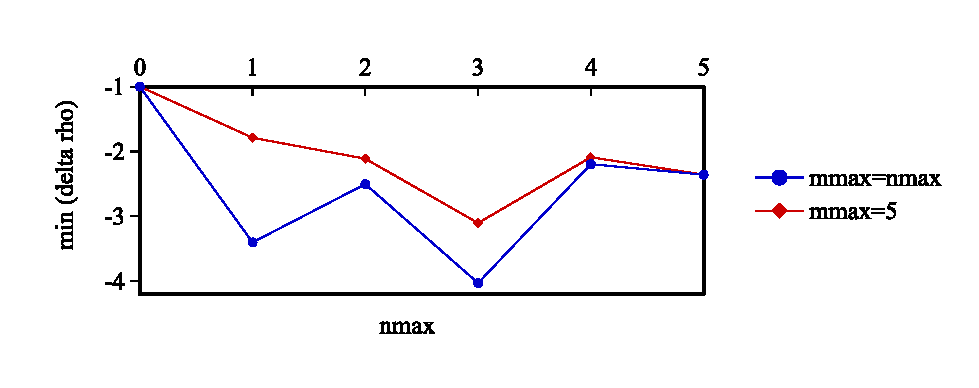
\includegraphics[bb=0bp 10bp 454bp 160bp,width=0.75\columnwidth]{_figure/results/min_delta_rho}
\par\end{centering}
\caption[The minimum value of $\Delta\rho(\mathbf{r},\mathbf{\Omega})/\rho_{0}$
after a forward-backward \acs{GSHT} process]{The minimum value of $\Delta\rho(\mathbf{r},\mathbf{\Omega})/\rho_{0}$
after a forward-backward \acs{GSHT} process with respect to $n_{\max}$.
Computed for a $45^{3}$ grid ($L=25$) for a converged density of
an artificial charged LJ center $\mathrm{CH}_{4}^{+0.4}$. \label{fig:unphysical-rho} }
\end{figure}

Theoretically, we expect this minimum value approach to zero when
increasing $m_{\max}$ or $n_{\max}$, which is not exactly the case.
That means perhaps the order of expansion is still far from to find
a tendency. Knowing that $\rho(\mathbf{r},\mathbf{\Omega})/\rho_{0}\rightarrow0$
at center of the solute and $\rho(\mathbf{r},\mathbf{\Omega})/\rho_{0}\rightarrow1$
far from the solute, the error can be said oblivious within the computing
capacity ($n_{\max}<5$), that means we cannot expand rightly the
density $\rho$ on \acs{GSH} projections, where. But this have a
much less effect on the functional gradient $\gamma$ that we evaluate,
because in a convolution product, $\Delta\hat{\rho}(\mathbf{k},\mathbf{\Omega})$
and the \acs{DCF} $\hat{c}(k,\mathbf{\Omega}_{1},\mathbf{\Omega}_{2})$
can be both expended, and product of higher order terms vanishes more
easily. Latter we will show that the profile of $\gamma$ and the
free energy $\mathcal{F}_{\mathrm{exc}}$ can already converge within
$n_{\max}<5$.

\section{Comparison between branches}

As shown in figure \ref{fig:Possible-algorithms}, if we fixe $\Delta\rho(\mathbf{r},\mathbf{\Omega})$
to a recombination of \acs{GSH} projections, all methods using the
same \acs{DCF} should give mathematically identical results. The
most direct comparison is the free energy evaluated during 1 iteration.
And to be more strict, is also interesting to compare the profile
of $\gamma$.

\subsection{Difference in energy evaluation}

As shown in table \ref{tab:free-energy}, the methods using the same
\acs{DCF} at the same $m_{\max}$ which is mathematically identical
in an infinite condition, give nearly the same results.

\begin{table}[H]
\begin{centering}
\begin{tabular*}{1\linewidth}{@{\extracolsep{\fill}}llll}
\toprule 
\tableheadline{Method} & $n_{\max}$ & \tableheadline{DCF} & \tableheadline{Free Energy} {\footnotesize{}(kJ/mol)}\tabularnewline
\midrule
\texttt{\textbf{\footnotesize{}dipole}} & {\footnotesize{}1} & {\footnotesize{}{[}ref mdft{]}} & {\footnotesize{}13.1915264499904339}\tabularnewline
\texttt{\textbf{\footnotesize{}naive\_dipole}} & {\footnotesize{}1} & {\footnotesize{}{[}ref mdft{]}} & {\footnotesize{}13.1915269013357985}\tabularnewline
\midrule 
\texttt{\textbf{\footnotesize{}naive\_nmax1}} & {\footnotesize{}1} & {\footnotesize{}\citep{puibasset_bridge_2012}{*}} & {\footnotesize{}18.6052247636086854}\tabularnewline
\texttt{\textbf{\footnotesize{}convolution\_standard}} & {\footnotesize{}1} & {\footnotesize{}\citep{puibasset_bridge_2012}{*}} & {\footnotesize{}18.6093390102806886}\tabularnewline
\midrule 
\texttt{\textbf{\footnotesize{}naive\_interpolation}} & {\footnotesize{}2} & {\footnotesize{}\citep{puibasset_bridge_2012}} & {\footnotesize{}26.8444355457069044}\tabularnewline
\texttt{\textbf{\footnotesize{}naive\_standard}} & {\footnotesize{}2} & {\footnotesize{}\citep{puibasset_bridge_2012}} & {\footnotesize{}26.9897310488084479}\tabularnewline
\texttt{\textbf{\footnotesize{}convolution\_standard}} & {\footnotesize{}2} & {\footnotesize{}\citep{puibasset_bridge_2012}} & {\footnotesize{}26.9163932581793155}\tabularnewline
\texttt{\textbf{\footnotesize{}convolution\_asymm}} & {\footnotesize{}2} & {\footnotesize{}\citep{puibasset_bridge_2012}} & {\footnotesize{}26.9163932581793155}\tabularnewline
\texttt{\textbf{\footnotesize{}convolution\_pure\_angular}} & {\footnotesize{}2} & {\footnotesize{}\citep{puibasset_bridge_2012}} & {\footnotesize{}26.9163932581793155}\tabularnewline
\bottomrule
\end{tabular*}
\par\end{centering}
\caption[Free energy calculated during 1 iteration]{Free energy calculated during 1 iteration for a $32^{3}$ grid ($L=20\textrm{Å}$)
for a fake LJ center $\mathrm{CH_{4}^{+0.33}}$, using a converged
density as input. Here $m_{\max}=n_{\max}$. \textcolor{red}{``{*}''
means ancient DCF, not so much difference.}\label{tab:free-energy}}
\end{table}
 

The light difference between \texttt{\textbf{naive\_nmax1}} and \texttt{\textbf{convolution\_standard}}
at $m_{\max}=1$ is due to the artificial decoration at $k$-border
showing in later section, and the difference between \texttt{\textbf{naive\_interpolation}}
and \texttt{\textbf{naive\_standard}} and \texttt{\textbf{convolution}}
methods are also acceptable, which is natural to be lightly different
due to the interpolation error and the \acs{GSH} expansion (the $\rho$
recombination of \acs{GSH} projections will be discussed later).
This supports by the way that we do not need the same order of \acs{GSH}
expansion for $\gamma$ than for $\Delta\rho$.

\subsection{A single k-kernel\label{subsec:A-single-k-kernel}}

Firstly, we are interested in the local paths from $\Delta\hat{\rho}_{\mu'\mu}^{m}(\mathbf{k})$
to $\hat{\gamma}_{\mu'\mu}^{m}(\mathbf{k})$ , that can be tested
independently for a certain $\mathbf{k}$. As shown in figure \ref{fig:k-kernel},
four algorithms are available to the purpose.

\begin{figure}[h]
\begin{centering}
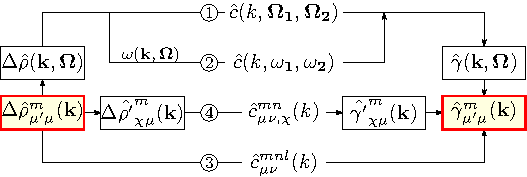
\includegraphics{_figure/algorithms_q}
\par\end{centering}
\caption{Schema of a k-kernel test \label{fig:k-kernel} }
\end{figure}

The program that compares each element of $\hat{\gamma}_{\mu'\mu}^{m}(\mathbf{k})$
issued from these 4 algorithms for a given $\Delta\hat{\rho}_{\mu'\mu}^{m}(\mathbf{k})$
is done by Mr. Luc Belloni, which shows that the $\hat{\gamma}_{\mu'\mu}^{m}(\mathbf{k})$
for the four algorithms are strictly identical. This means, the final
result of energy and structure is independent to the choice of path
inside a $k$-kernel, if $\Delta\hat{\rho}(\mathbf{k},\mathbf{\Omega})$
can be fully expended on \acs{GSH}s.

\subsection{k-border effect\label{subsec:k-border-effect}}

Here we test the whole process shown in figure \ref{fig:Possible-algorithms},
with $\Delta\rho(\mathbf{r},\mathbf{\Omega})$ generated from a recombination
of \acs{GSH} projections. Firstly, we compare the three \texttt{\textbf{convolution}}
algorithms passing by \acs{GSH} expansion. For a $64^{3}$ grid,
$n_{\max}=3$, the three algorithms \texttt{\textbf{convolution\_standard}},
\texttt{\textbf{convolution\_asymm}}, and \texttt{\textbf{convolution\_pure\_angular}}
gives the same free energy, but lightly different result when comparing
each element of $\gamma(\mathbf{r},\mathbf{\Omega})$, and this difference
seems to decrease when increase the number of grid points. More, the
projections $\gamma_{\mu'\mu}^{m}(\mathbf{r})$ which should be purely
real as explained in $\mathsection$\ref{subsec:Reduction-by-symmetry},
have a light imaginary part. But surprisingly, for a $65^{3}$ grid,
it gives numerically the same result for both the three algorithms
at machine precision.{*} \marginpar{{*} The detailed value of $\gamma$ which the paragraph of description
is based on haven't been noted, as it was regarded as a bug in the
code at that time, and the code had been then modified; and to redo
such a process takes a lot of time.}

The difference between these methods is found to be a special $k$-border
effect linking to even number grids.

As the symmetry
\begin{equation}
\Delta\hat{\rho'}_{\chi\mu}^{m}(\mathbf{k})=(-)^{m+\mu+\chi}\Delta\hat{\rho'}_{\chi,-\mu}^{m*}(-\mathbf{k})\label{eq:2-1}
\end{equation}
 is generated by two symmetries
\begin{equation}
\Delta\hat{\rho}_{\mu'\mu}^{m}(\mathbf{k})=(-)^{\mu'+\mu}\Delta\hat{\rho}_{-\mu',-\mu}^{m*}(-\mathbf{k})\label{eq:1-1}
\end{equation}
\begin{equation}
R_{\mu'\chi}^{m}(\hat{k})=(-)^{m+\mu'+\chi}R_{-\mu',\chi}^{m}(-\hat{k})\label{eq:3-1}
\end{equation}

For the points ``at border'', it's to say that after the FFT where
the point having $\pm k_{i}=k_{i}^{\mathrm{max}}$, $i=1,2,3$, for
example for $k_{1},$

\[
\Delta\hat{\rho}_{\mu'\mu}^{m}(\pm k_{1},k_{2},k_{3})=\Delta\hat{\rho}_{\mu'\mu}^{m}(k_{1}^{\mathrm{max}},k_{2},k_{3})
\]
is naturally put in the same array by FFT for the grids having even
number,\marginpar{For example, for a grid 1D, the FFT having 6 points gives the values
for indices 0,1,2,3,-2,-1, and the FFT having 7 points gives the values
for 0,1,2,3,-3,-2,-1.} as shown in figure \ref{fig:k-border-effect}. 

\begin{figure}[h]
\begin{centering}
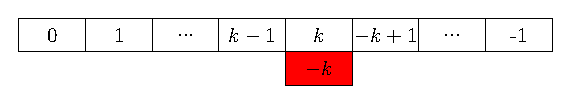
\includegraphics{_figure/k-border}
\par\end{centering}
\caption{$k$-border effect\label{fig:k-border-effect}}
\end{figure}

As \acs{FFT} possesses periodicity, the symmetry \ref{eq:1-1} can
always be respected at border. However, as
\begin{equation}
R_{-\mu',\chi}^{m}(-\hat{k}\equiv(-k_{1},-k_{2},-k_{3}))\neq R_{\mu',\chi}^{m}(k_{1}^{\mathrm{max}},-k_{2},-k_{3})
\end{equation}
the symmetries (\ref{eq:3-1}) and (\ref{eq:2-1}) are not respected
for these points. In the backward process, if we make sense of all
the $\gamma_{\mu'\mu}^{m}(\mathbf{k})$, as
\[
\gamma_{\mu'\mu}^{m}(-\hat{k}\equiv(-k_{1},-k_{2},-k_{3}))\neq\gamma_{\mu'\mu}^{m}(k_{1}^{\mathrm{max}},-k_{2},-k_{3})
\]
the symmetry
\begin{equation}
\gamma_{\mu'\mu}^{m}(\mathbf{k})=(-)^{\mu'+\mu}\gamma_{-\mu',-\mu}^{m*}(-\mathbf{k})\label{eq:1-1}
\end{equation}
is not respected totally, and this imposes that $\gamma_{\mu'\mu}^{m}(\mathbf{r})$
have a imaginary part. This imaginary part has been omitted implicitly
in the ``real to complex'' \acs{FFT} process of used in for example
\texttt{\textbf{convolution\_standard}}, for \acs{FGSHT}, or \texttt{\textbf{convolution\_pure\_angular}}
for FFT3D process. It is to say, we keep only the part of none-negative
$\mathbf{k}$ or none-negative $\mu$, supposing that the part we
omit respects the symmetry.

The right way to treat this issue is to artificially impose at the
border:
\begin{equation}
R_{\mu',\chi}^{m}(k_{i}^{\mathrm{max}})=\frac{1}{2}\left[R_{\mu',\chi}^{m}(k_{i})+R_{\mu',\chi}^{m}(-k_{i})\right]
\end{equation}
where $i$ is the conflict index in figure \ref{fig:k-border-effect}.
If more than one dimensions are in conflict, this process can be done
twice (4 terms for ``edges'' of the cube) or three times (8 terms
for ``vertices''). The point $\mathbf{k}=\hat{0}$ is different,
as it was define along $z$ axes to avoid implementation crash, it
doesn't respect eq. (\ref{eq:3-1}) and (\ref{eq:2-1}) neither. But
this point compared to hundreds thousands of total points is negligible.

The energies given by \texttt{\textbf{naive\_standard}} and the \texttt{\textbf{convolution}}
algorithms are identical for a $65^{3}$ and $n_{\max}=3$ grid, but
the element of $\gamma(\mathbf{r},\mathbf{\Omega})$ have a mysterious
difference at order of $10^{-2}$, seemed to be aleatory. A test redone
for a $45^{3}$ grid is shown in figure \ref{fig:Difference-in-gamma}.

\begin{figure}[H]
\begin{centering}
\subfloat[$\delta\hat{\gamma}(\mathbf{k},\mathbf{\Omega})$]{\begin{centering}
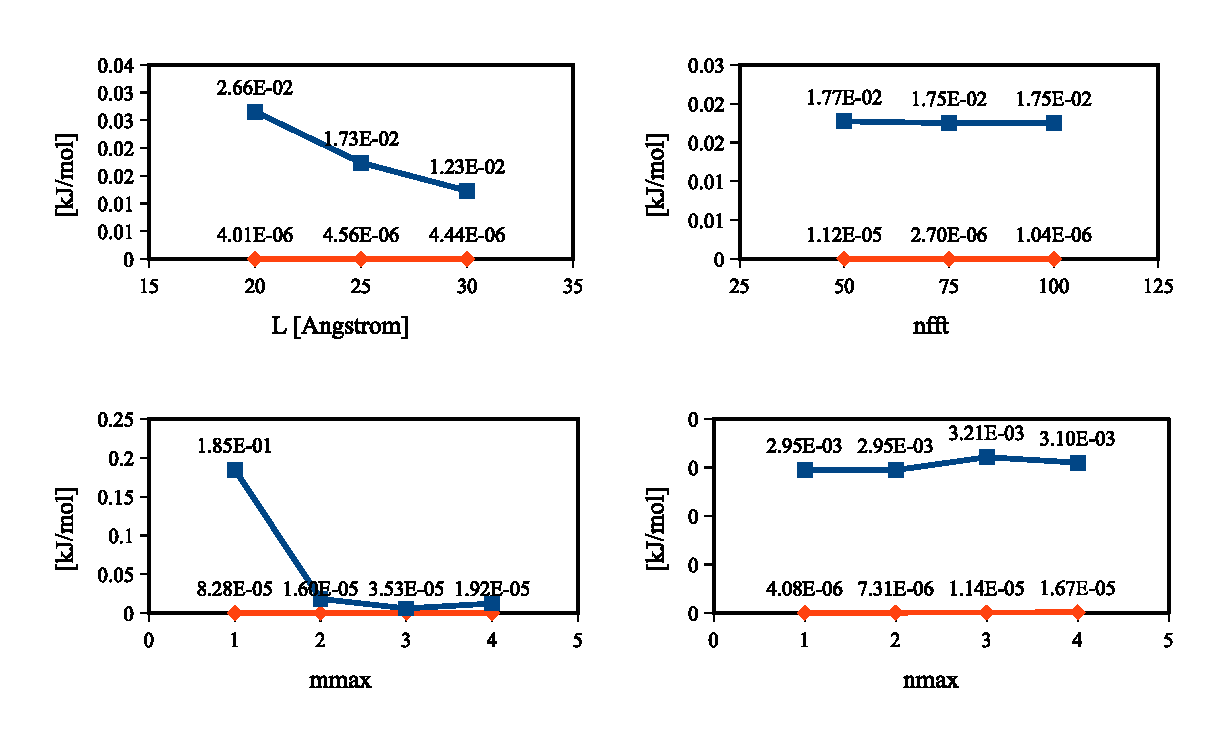
\includegraphics[width=0.75\columnwidth]{_figure/results/diff_k_gamma}
\par\end{centering}

}
\par\end{centering}
\begin{centering}
\subfloat[$\delta\gamma(\mathbf{r},\mathbf{\Omega})$]{\begin{centering}
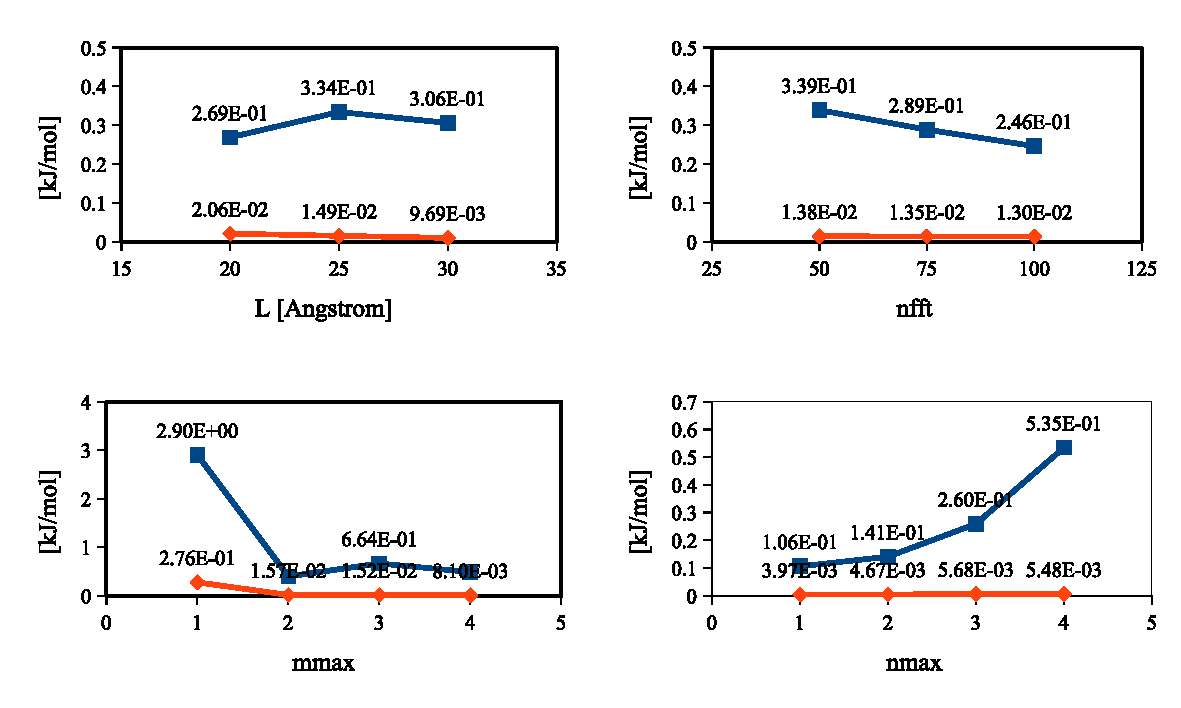
\includegraphics[width=0.75\columnwidth]{_figure/results/diff_gamma}
\par\end{centering}
}
\par\end{centering}
\caption[Maximum and average difference in $\hat{\gamma}(\mathbf{k},\mathbf{\Omega})$
and $\gamma(\mathbf{r},\mathbf{\Omega})$]{Maximum and average difference in $\hat{\gamma}(\mathbf{k},\mathbf{\Omega})$
and $\gamma(\mathbf{r},\mathbf{\Omega})$, for tests of different
box length$L$, different number of grid nfft in one dimension, $n_{\max}=1,4$
for $m_{\max}=n_{\max}$, and $n_{\max}=1,4$ for $m_{\max}=5$.\label{fig:Difference-in-gamma}}
\end{figure}

We can conclude very rudely that this error depends on the angular
quadrature $m_{\max}$. The dependence is natural, as the difference
between algorithms \texttt{\textbf{naive}} and \texttt{\textbf{convolution}}
is the treatment of the angular part. There is also a dependence on
$L$ in the $k$-space, but after \acs{FFT} it is mixed. The augmentation
of error in the $n_{\max}$ chart is unnatural, implying there is
perhaps a still bug in the code.

In a word, this mysterious difference cannot be yet explained, as
the \texttt{\textbf{naive}} methods does not have the $k$-border
effect linked to symmetry, on the other hand we used a odd grid, we
could not yet distinguish that it is a bug in the implementation,
in the test or in the theory. The projections $\gamma_{\mu\nu}^{mnl}(r)$
of this two algorithms seems to be identical (figure \ref{fig:gamma-proj}),
it is to say, the global structure of this two algorithms are almost
the same, and the error would not be very decisive.

\begin{figure}[h]
\begin{centering}
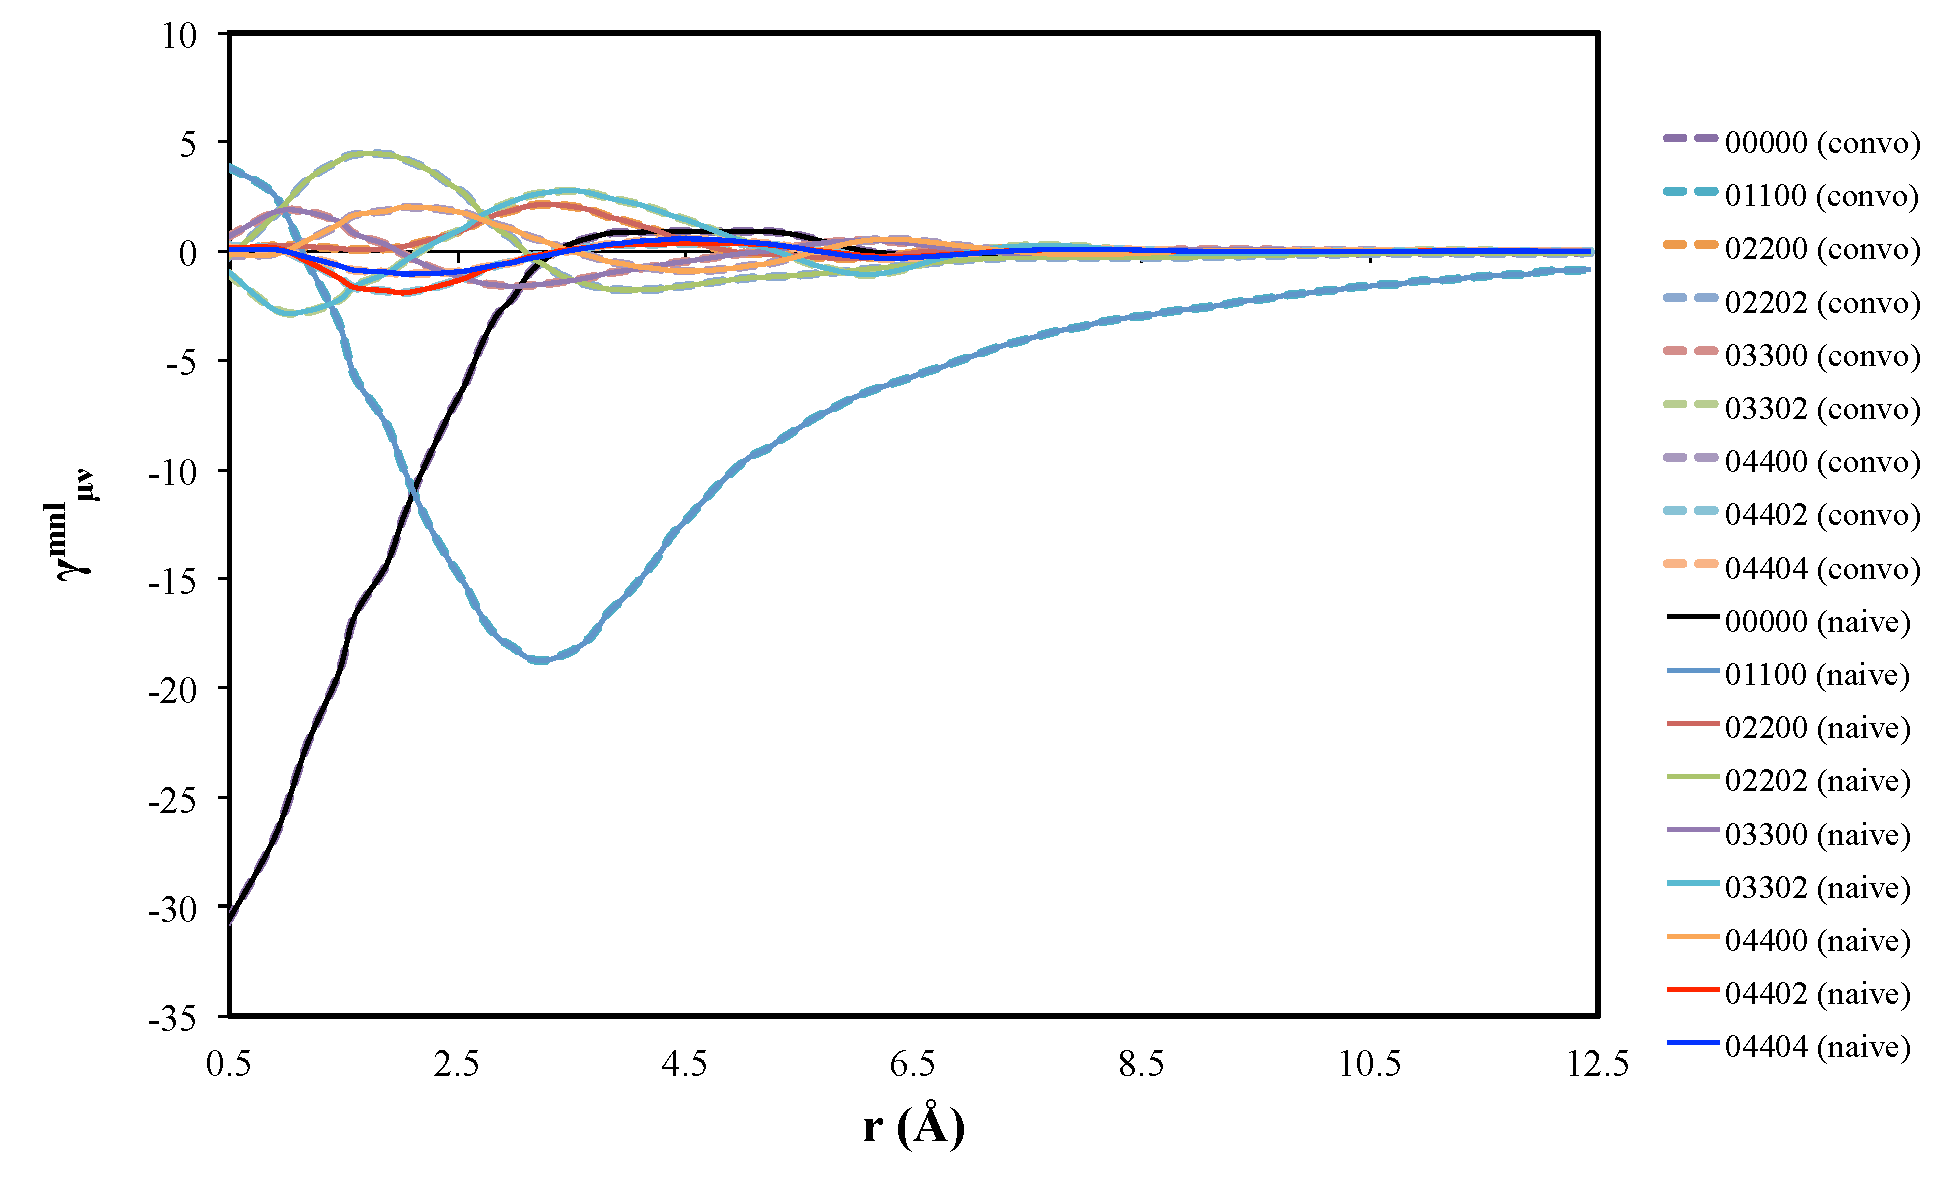
\includegraphics[width=0.65\columnwidth]{_figure/results/gamma_proj}
\par\end{centering}
\caption{A selection of rotational invariant projections $\gamma_{\mu\nu}^{mnl}(r)$
for a $65^{3}$ grid\label{fig:gamma-proj}}
\end{figure}


\section{Intrinsic variation of free energy\label{sec:Intrinsic-variation-of}}

Before study of free energy dependence on angular algorithms, we are
interested in the grid dependance, with can have an influence to the
tests later.

\begin{figure}[H]
\begin{centering}
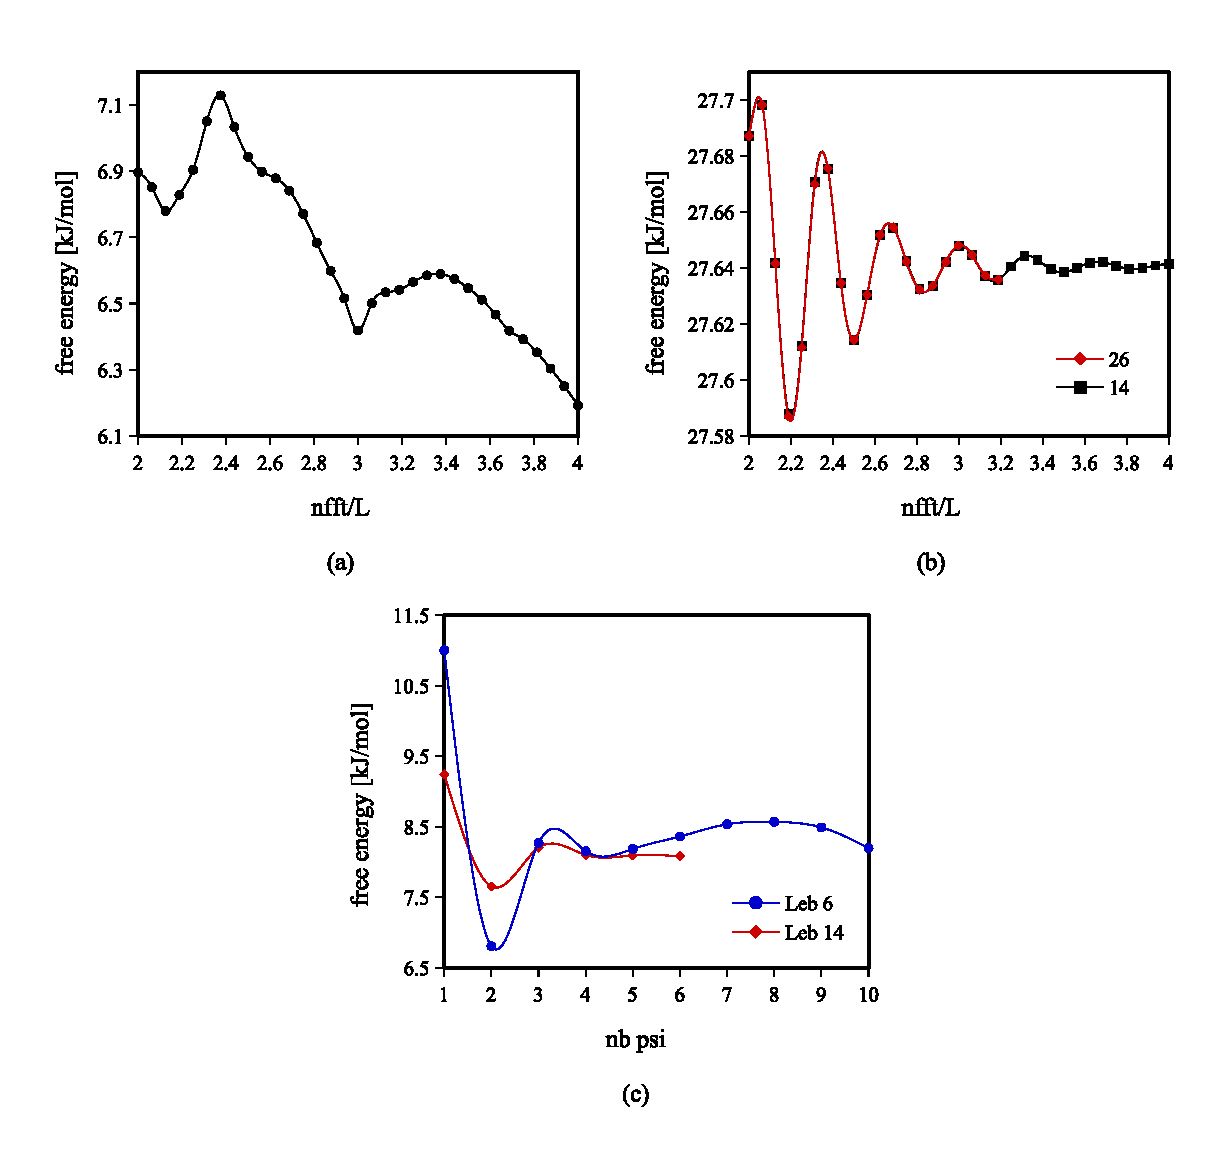
\includegraphics[bb=0bp 20bp 567bp 519bp,width=0.75\columnwidth]{_figure/results/grid_reso}
\par\end{centering}
\caption[Space-grid and $\Psi$ dependence of code MDFT]{Space-grid and $\Psi$ dependence of code MDFT. $L=32$. (a) $\mathrm{CH_{4}^{+0.33}}$
using dipole DCF with $m_{\max}=1$; (b) $\mathrm{CH_{4}}$ using
DCF of $m_{\max}=5$, Lebedev quadrature of order 1 and 2; (c) acetone
using dipole DCF and Lebedev quadrature, varying $\Psi$, nfft=128.
\label{fig:Space-grid-and-psi-dependence}}
\end{figure}

As shown in figure \ref{fig:Space-grid-and-psi-dependence} (a) and
(b), there is a dependence of calculated free energy on the space
grid resolution. for a charged solute, the energy has tendency to
decrease when increasing the resolution of grid (nfft). And this decrease
does not link to the border correction mentioned in $\mathsection$\ref{chpt:thermodynamic-quantities},
as the box length and the charge remain the same for the whole set
of test. From (b) we consider that at least 3 points grid in one dimension
per Angstrom is needed to reduce the uncertainty due to grid resolution.
Figure (c) fixed the Lebedev quadrature for $\Theta$ and $\Phi$,
but leaved varying the $\Psi$. We can also see a dependence on $\Psi$.
which does not vanish when increasing the resolution of grid. As during
the whole thesis the $\Psi$ is theoretically fixed in the same order
with $\Theta$ and $\Phi$, this remains an issue for further verification.
We can roughly conclude that an error around 1 kJ/mol is common for
this code.

\section{Series of charged LJ centre}

To valid the method, we chose a series of LJ centre, which possess
the LJ parameters of $\mathrm{C}\mathrm{H}_{4}$ in \textcolor{red}{{[}ref{]}},
and have a various charge from -1.0 to 1.0 (table \ref{tab:Parameters-of-charged-met}).\marginpar{For both IET, and DM results, 298K is used according to habitude instead
of 303K recommended in reference \citep{SPC/E}. For MDFT, 300K and
298K are used.}

\begin{table}[h]
\begin{centering}
\begin{tabular*}{1\linewidth}{@{\extracolsep{\fill}}lllllll}
\toprule 
\tableheadline{Charge} & $\sigma$ {[}$\textrm{Å}${]} & $\epsilon$ {[}$\mathrm{kJ\cdot mol^{-1}}${]} & $x$ {[}$\textrm{\AA}${]} & $y$  {[}$\textrm{\AA}${]} & $z$ {[}$\textrm{\AA}${]} & \tableheadline{Number Density} {[}$\lyxmathsym{\AA}^{-3}${]}\tabularnewline
\midrule
-1.0 to 1.0 & 3.73  & 1.23  & 0 & 0 & 0 & 0.0332891 \textcolor{red}{{[}ref,temperature{]}}\tabularnewline
\bottomrule
\end{tabular*}
\par\end{centering}
\caption{Parameters of charged Lenard-Jones centre (modified from $\mathrm{C}\mathrm{H}_{4}$)
\label{tab:Parameters-of-charged-met}}
\end{table}


\subsection{Box length dependance and charge dependance of free energy}

As discussed in section \ref{chpt:thermodynamic-quantities}, for
single ions, two types of corrections need to be added on the free
energy, which depend on the box length and and charge of the ion.
To verify these dependence, we implement a systematic calculation
from charge, using 3 different methods, where the parameters are shown
in table \ref{tab:parameters-ch4}. It should be noted that, the \texttt{\textbf{naive\_interpolation}}
only used 14 Lebedev and 3 $\Psi$ angles to converge, which gives
exactly the same result with 26 Lebedev and 4 $\Psi$ angles, that
means, the \texttt{\textbf{naive}} methods do not need an order of
quadrature $m_{\max}$ to be greater than the order of DCF $n_{\max}$.
The -1 side has problem of convergence, and all the converged results
are presented.

\begin{table}[h]
\begin{centering}
\begin{tabular*}{1\linewidth}{@{\extracolsep{\fill}}llll}
\toprule 
\tableheadline{Method} & nfft/$L$ & $m_{\max}$ & $n_{\max}$\tabularnewline
\midrule
\texttt{\textbf{naive\_nmax1}} & 3 & 1 & 1\tabularnewline
\texttt{\textbf{naive\_interpolation}} & 3 & 2 (Leb) & 5\tabularnewline
\texttt{\textbf{convolution\_standard}} & 3 & 1 & 1\tabularnewline
\bottomrule
\end{tabular*}
\par\end{centering}
\caption{Methods and parameters for $\mathrm{C}\mathrm{H}_{4}$ series test.
{*} Leb is Lebedev quadrature, with is mathematically equivalent with
Gauss-Legendre quadrature but only ˜2/3 angles.\label{tab:parameters-ch4}}
\end{table}

The direct results collection are shown in figure \ref{fig:ch4_nmax1_lmn},
\ref{fig:ch4_nmax5_inter} and \ref{fig:ch4_nmax1_new} at the end
of this section. We can see that the dependence of box length for
each charge is almost linear, except the charge between $\left[-0.2,0.2\right]$.
This means, the influence of box length is much greater than the intrinsic
variation of result that mentioned in \ref{sec:Intrinsic-variation-of}.
The charge dependency is traced in figure \ref{fig:Quadratic-charge-dependence},
using all the number of slopes with respect to the square of their
charge ($q^{2}$). A linear regression is done to give the slope 1937.8
$\mathrm{kJ}\cdot\mathrm{mol^{-1}}\cdot\textrm{Å}$. This slope correspond
to the correction of type-B (normalized to give the right unity):
\begin{equation}
\dfrac{\xi}{2}\left(1-\dfrac{1}{\varepsilon}\right)=1943.2\,\mathrm{kJ}\cdot\mathrm{mol^{-1}}\cdot\textrm{Å}
\end{equation}

\begin{figure}[H]
\begin{centering}
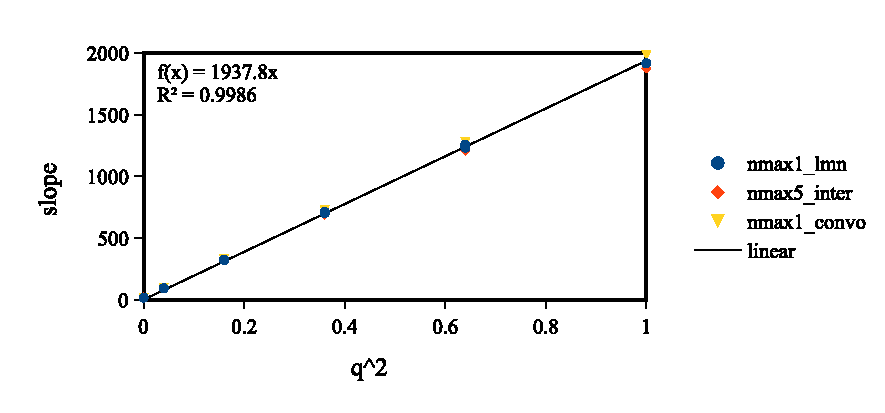
\includegraphics[bb=0bp 20bp 425bp 178bp,scale=0.6]{_figure/results/ch4_slope}
\par\end{centering}
\caption{Quadratic charge dependence of free energy of $\mathrm{C}\mathrm{H}_{4}$
centre series\label{fig:Quadratic-charge-dependence}}
\end{figure}
The intercept values in each of figure \ref{fig:ch4_nmax1_lmn} to
\ref{fig:ch4_nmax1_new} correspond to the free energy of an infinite
box. The \acs{IET} results are done with $R_{\max}=102.4\textrm{Å}$,
and need a correction of $-2.556k_{\mathrm{B}}T$. \textcolor{red}{(need
more details.)} The differences in free energy between MDFT and IET
are given in figure \ref{fig:Comparison-to-IET,without-correction}.
The linear regression is done with all existing points in this figure.
The slope 87.653 $\mathrm{kJ}\cdot\mathrm{mol^{-1}}$ corresponds
to the correction of type-C (normalized to give the right unity):
\begin{equation}
\eta\gamma=82.104\mathrm{kJ}\cdot\mathrm{mol^{-1}}\label{eq:eta-gamma}
\end{equation}
These two numbers are a little different, principally due to a lack
of point at the -1 side.

\begin{figure}[h]
\begin{centering}
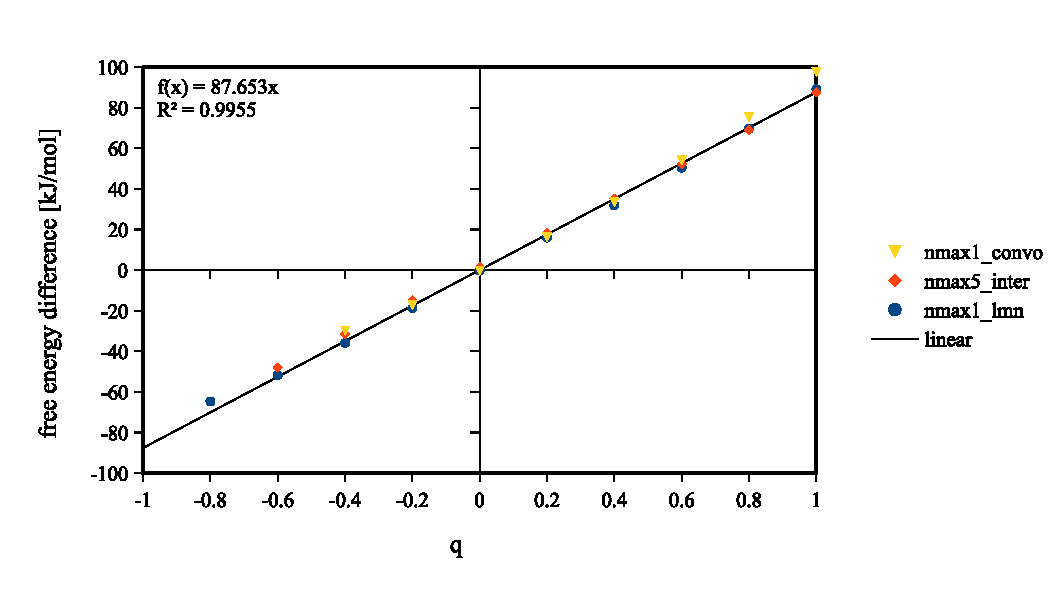
\includegraphics[bb=0bp 20bp 510bp 263bp,scale=0.6]{_figure/results/ch4_diff_energy}
\par\end{centering}
\caption{Comparison to IET, without P-scheme correction\label{fig:Comparison-to-IET,without-correction}}
\end{figure}


\subsection{Comparison with IET after corrections}

The figure \ref{fig:Comparison-to-IET,without-correction} after correction
with eq. (\ref{eq:eta-gamma}) gives figure \ref{fig:Comparison-to-IET,with-corr}.
It is shown that they are not perfectly agreed with each other. The
$n_{\max}=1$ methods have large difference when the charge increased,
especially the \texttt{\textbf{convolution\_standard}} using GSH expansion.
Knowing that during 1 iteration, the \texttt{\textbf{naive\_nmax1}}
and the \texttt{\textbf{convolution\_standard}} only give a slight
difference in free energy (table \ref{tab:free-energy}). The $n_{\max}=5$
have an energy shift about 2 $\mathrm{kJ}\cdot\mathrm{mol^{-1}}$,
which cannot have an explanation. but overall, to have 2 $\mathrm{kJ}\cdot\mathrm{mol^{-1}}$
per 100 $\mathrm{kJ}\cdot\mathrm{mol^{-1}}$ is already a good result.

\begin{figure}[H]
\begin{centering}
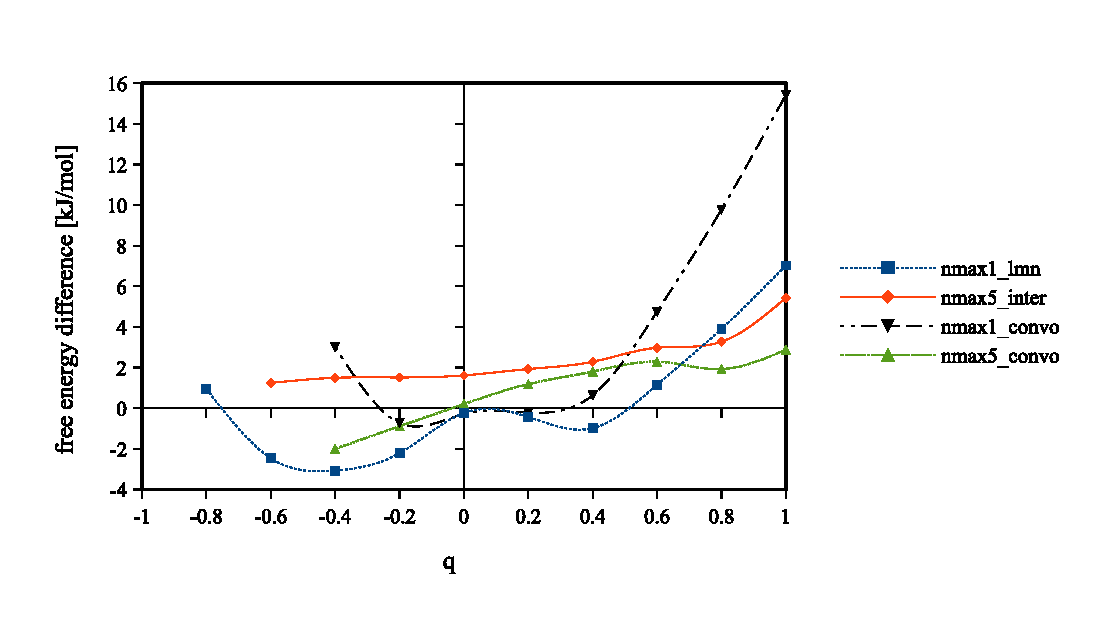
\includegraphics[bb=0bp 20bp 510bp 263bp,scale=0.6]{_figure/results/ch4_diff_inter}
\par\end{centering}
\caption{Comparison to IET, with P-scheme correction\label{fig:Comparison-to-IET,with-corr}}
\end{figure}

The case of $m_{\max}=5$ , $n_{\max}=0,\ldots,5$ with \texttt{\textbf{convolution\_standard}}
is shown in figure \ref{fig:Comparison-to-IET,nmax0-5}. It is interesting
to see how energy evaluate with $n_{\max}$ while fixing $m_{\max}$.
As we said, $\gamma$ is more smooth than $\rho$, that means we can
have $n_{\max}<m_{\max}$ to economize computing cost. Results shows
that within $n_{\max}\geq3$ for $n_{\max}=5$, the error is acceptable.
But again, the dependence on $q$ after correction is in incomprehensible.
And compared to \texttt{\textbf{naive\_interpolation}} in figure \ref{fig:Comparison-to-IET,with-corr},
we see that these error for $n_{\max}=5$ is different.

\begin{figure}[H]
\begin{centering}
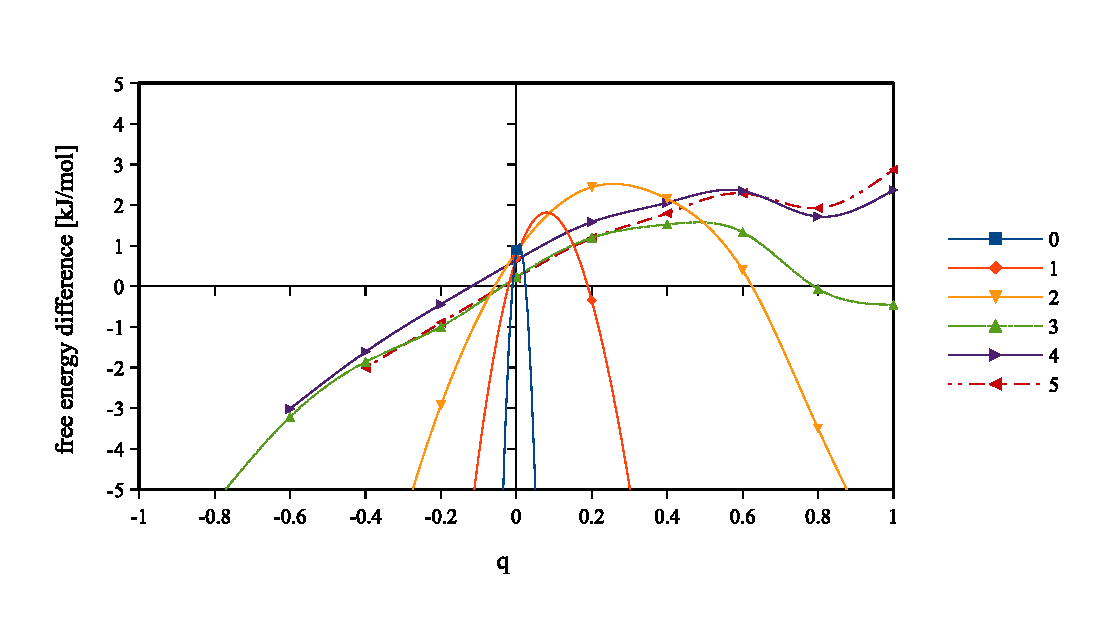
\includegraphics[bb=0bp 20bp 510bp 263bp,scale=0.6]{_figure/results/ch4_diff_mmax5}
\par\end{centering}
\caption{Comparison to IET, with P-scheme correction, $m_{\max}=5$ , $n_{\max}=0,\ldots,5$
\label{fig:Comparison-to-IET,nmax0-5}}
\end{figure}

The profile of $\rho$ can expended on rotational invariants which
is discussed in $\mathsection$\ref{chpt:solvation-structure}. The
comparison with IET is done for three charges, 0, -0.6 and +1. Shown
in figure \ref{fig:Comparison-to-IET.rot_invar}. Watch that the 0
and -1 one of $m_{\max}=5$ corresponds well the result of IEM, but
the -0.6 one have a lot of noise. (In fact, this configuration had
difficulty to converge, and the given energy is not good, thus it
is deleted in figure \ref{fig:Comparison-to-IET,nmax0-5}.) The the
profiles of go much better $m_{\max}=2,3$. Normally, more points
means more precision. It may means that with $m_{\max}=5$ , there
is perhaps a bug of integer overflow that prevent the convergence
for high charges.

\begin{figure}[H]
\begin{centering}
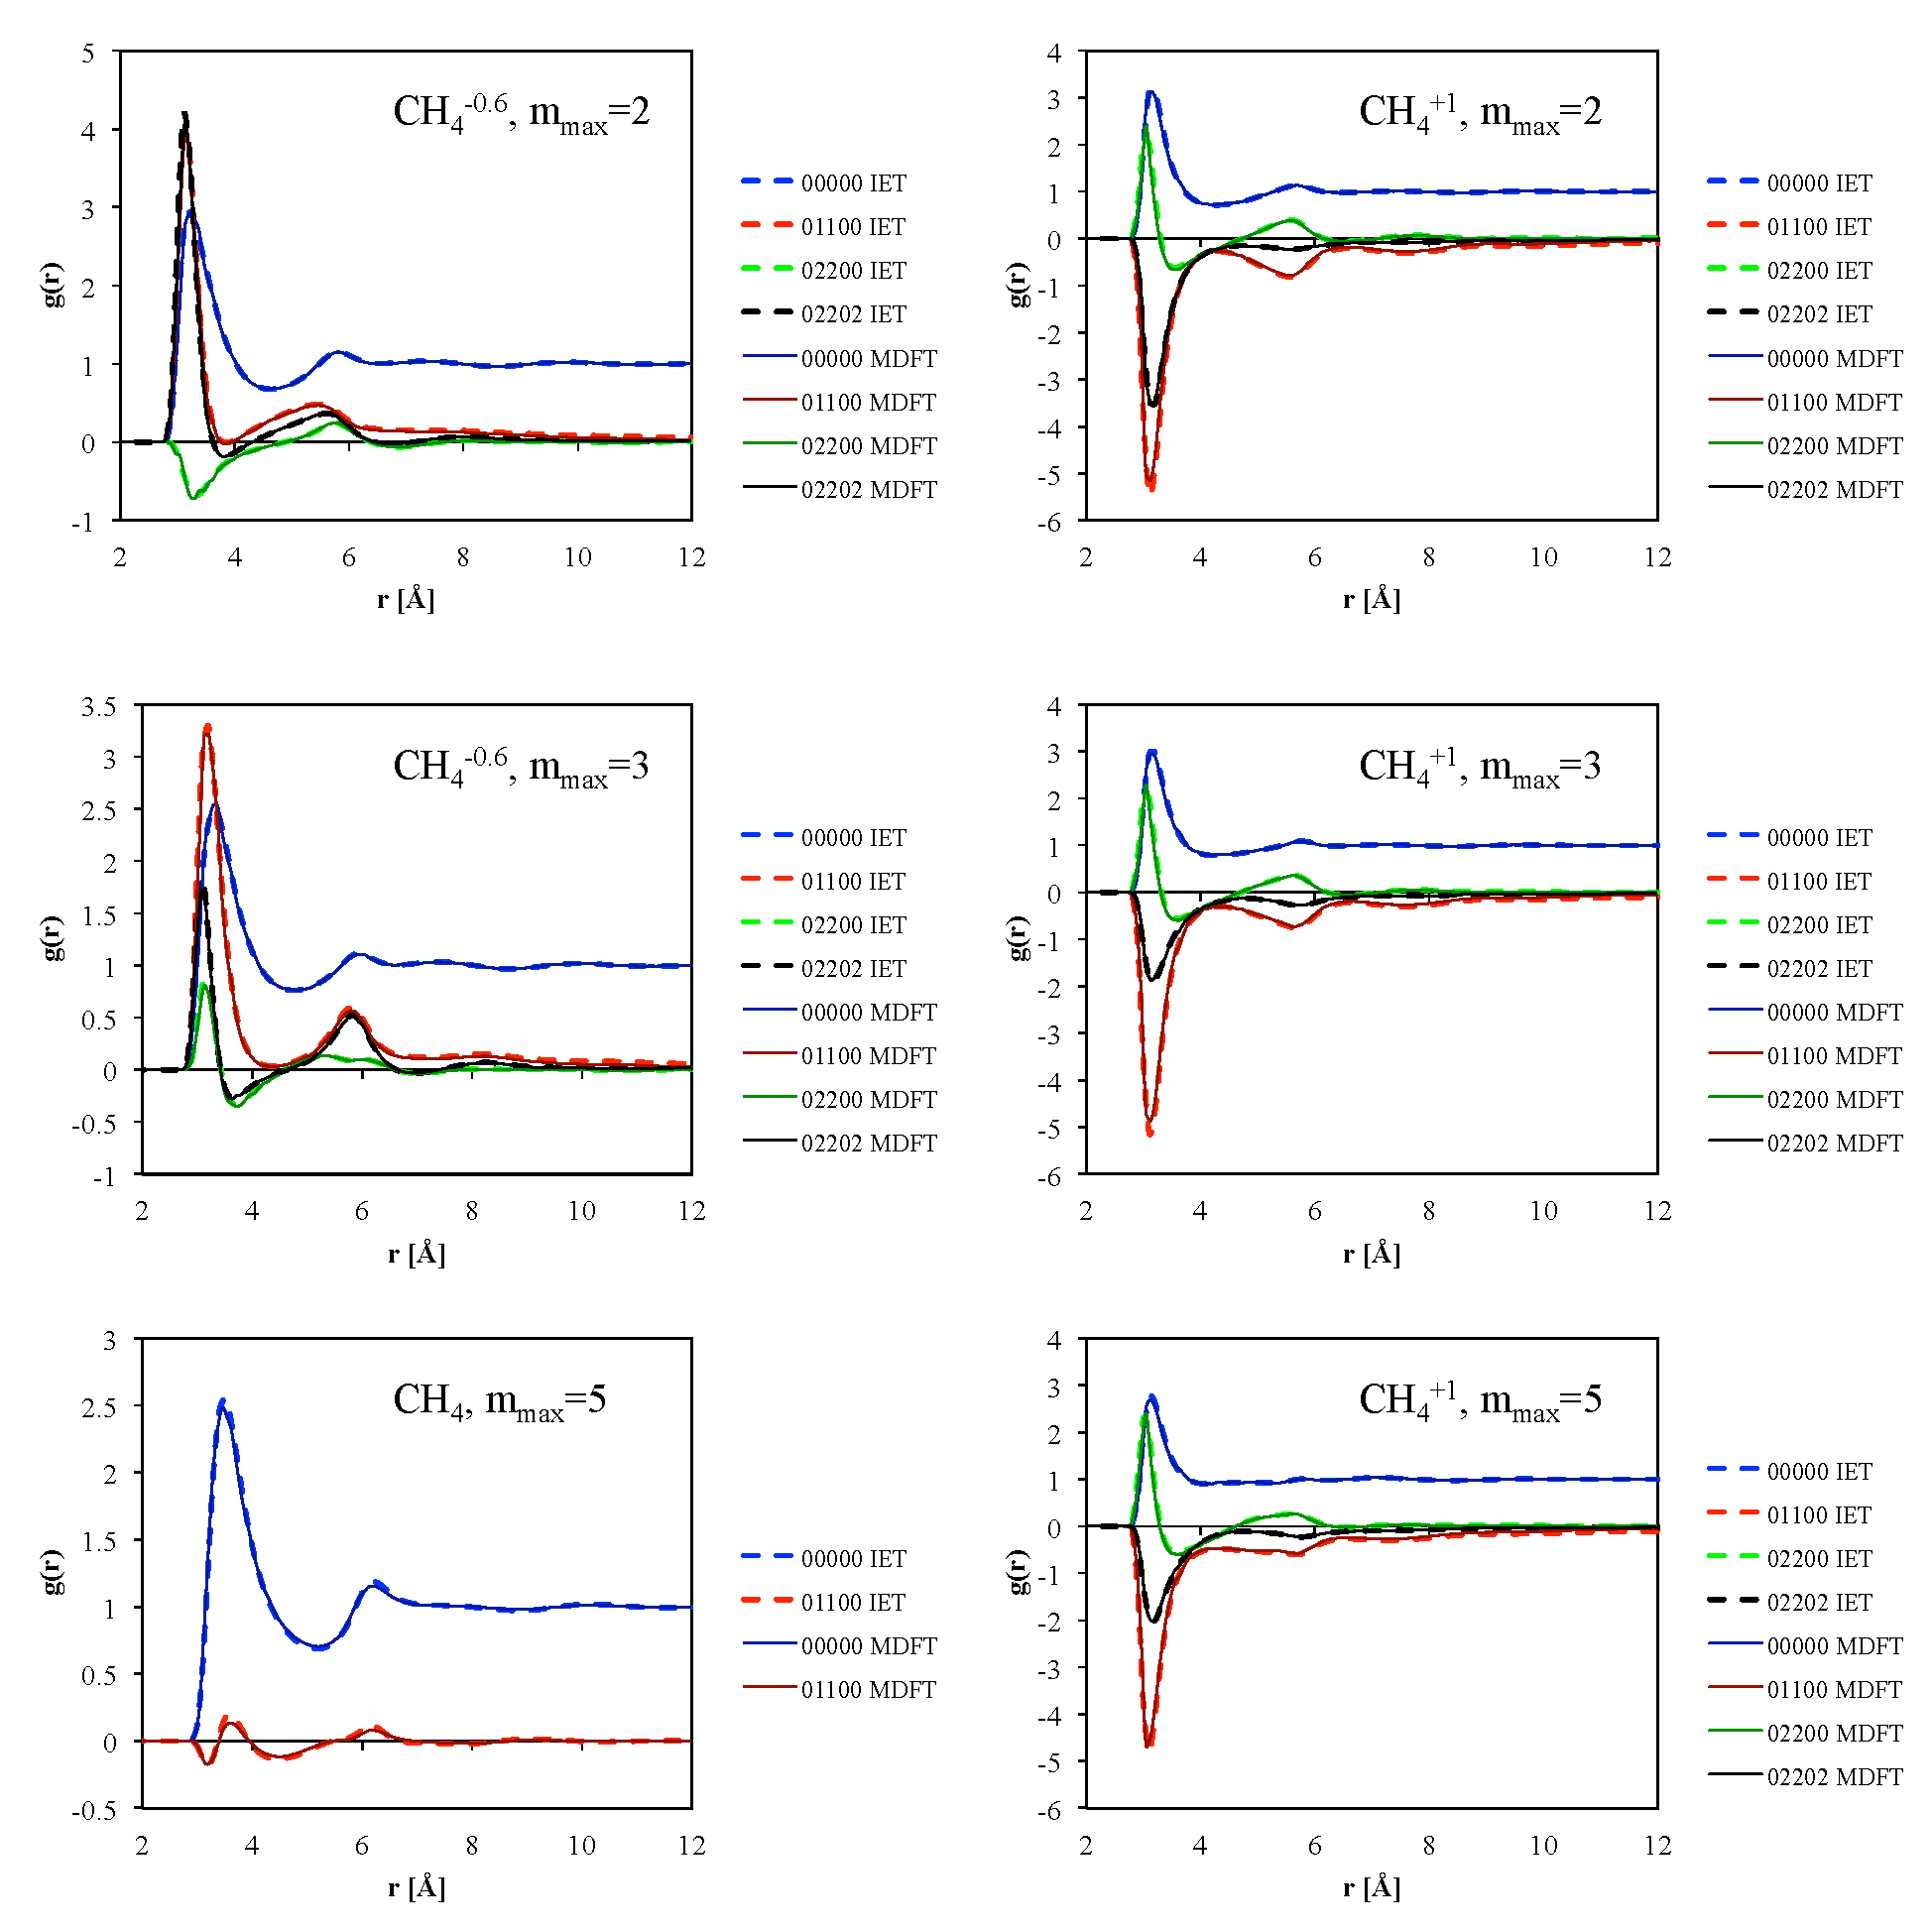
\includegraphics[width=1\columnwidth]{/Users/Hostiphre/Desktop/_M1102/_figure/results/ch4_iet_struct}
\par\end{centering}
\caption{Comparison to IET. Profile of $\rho$ in rotational invariant projections,
L=24, nfft=72.\label{fig:Comparison-to-IET.rot_invar}}
\end{figure}


\subsection{Comparison with MD}

The comparison of RDF with MD results are shown in figure \ref{fig:Comparison-to-MD}.
We can see that for negative charges, there are a lot of shifts.

Discussion...

\begin{figure}[H]
\begin{centering}
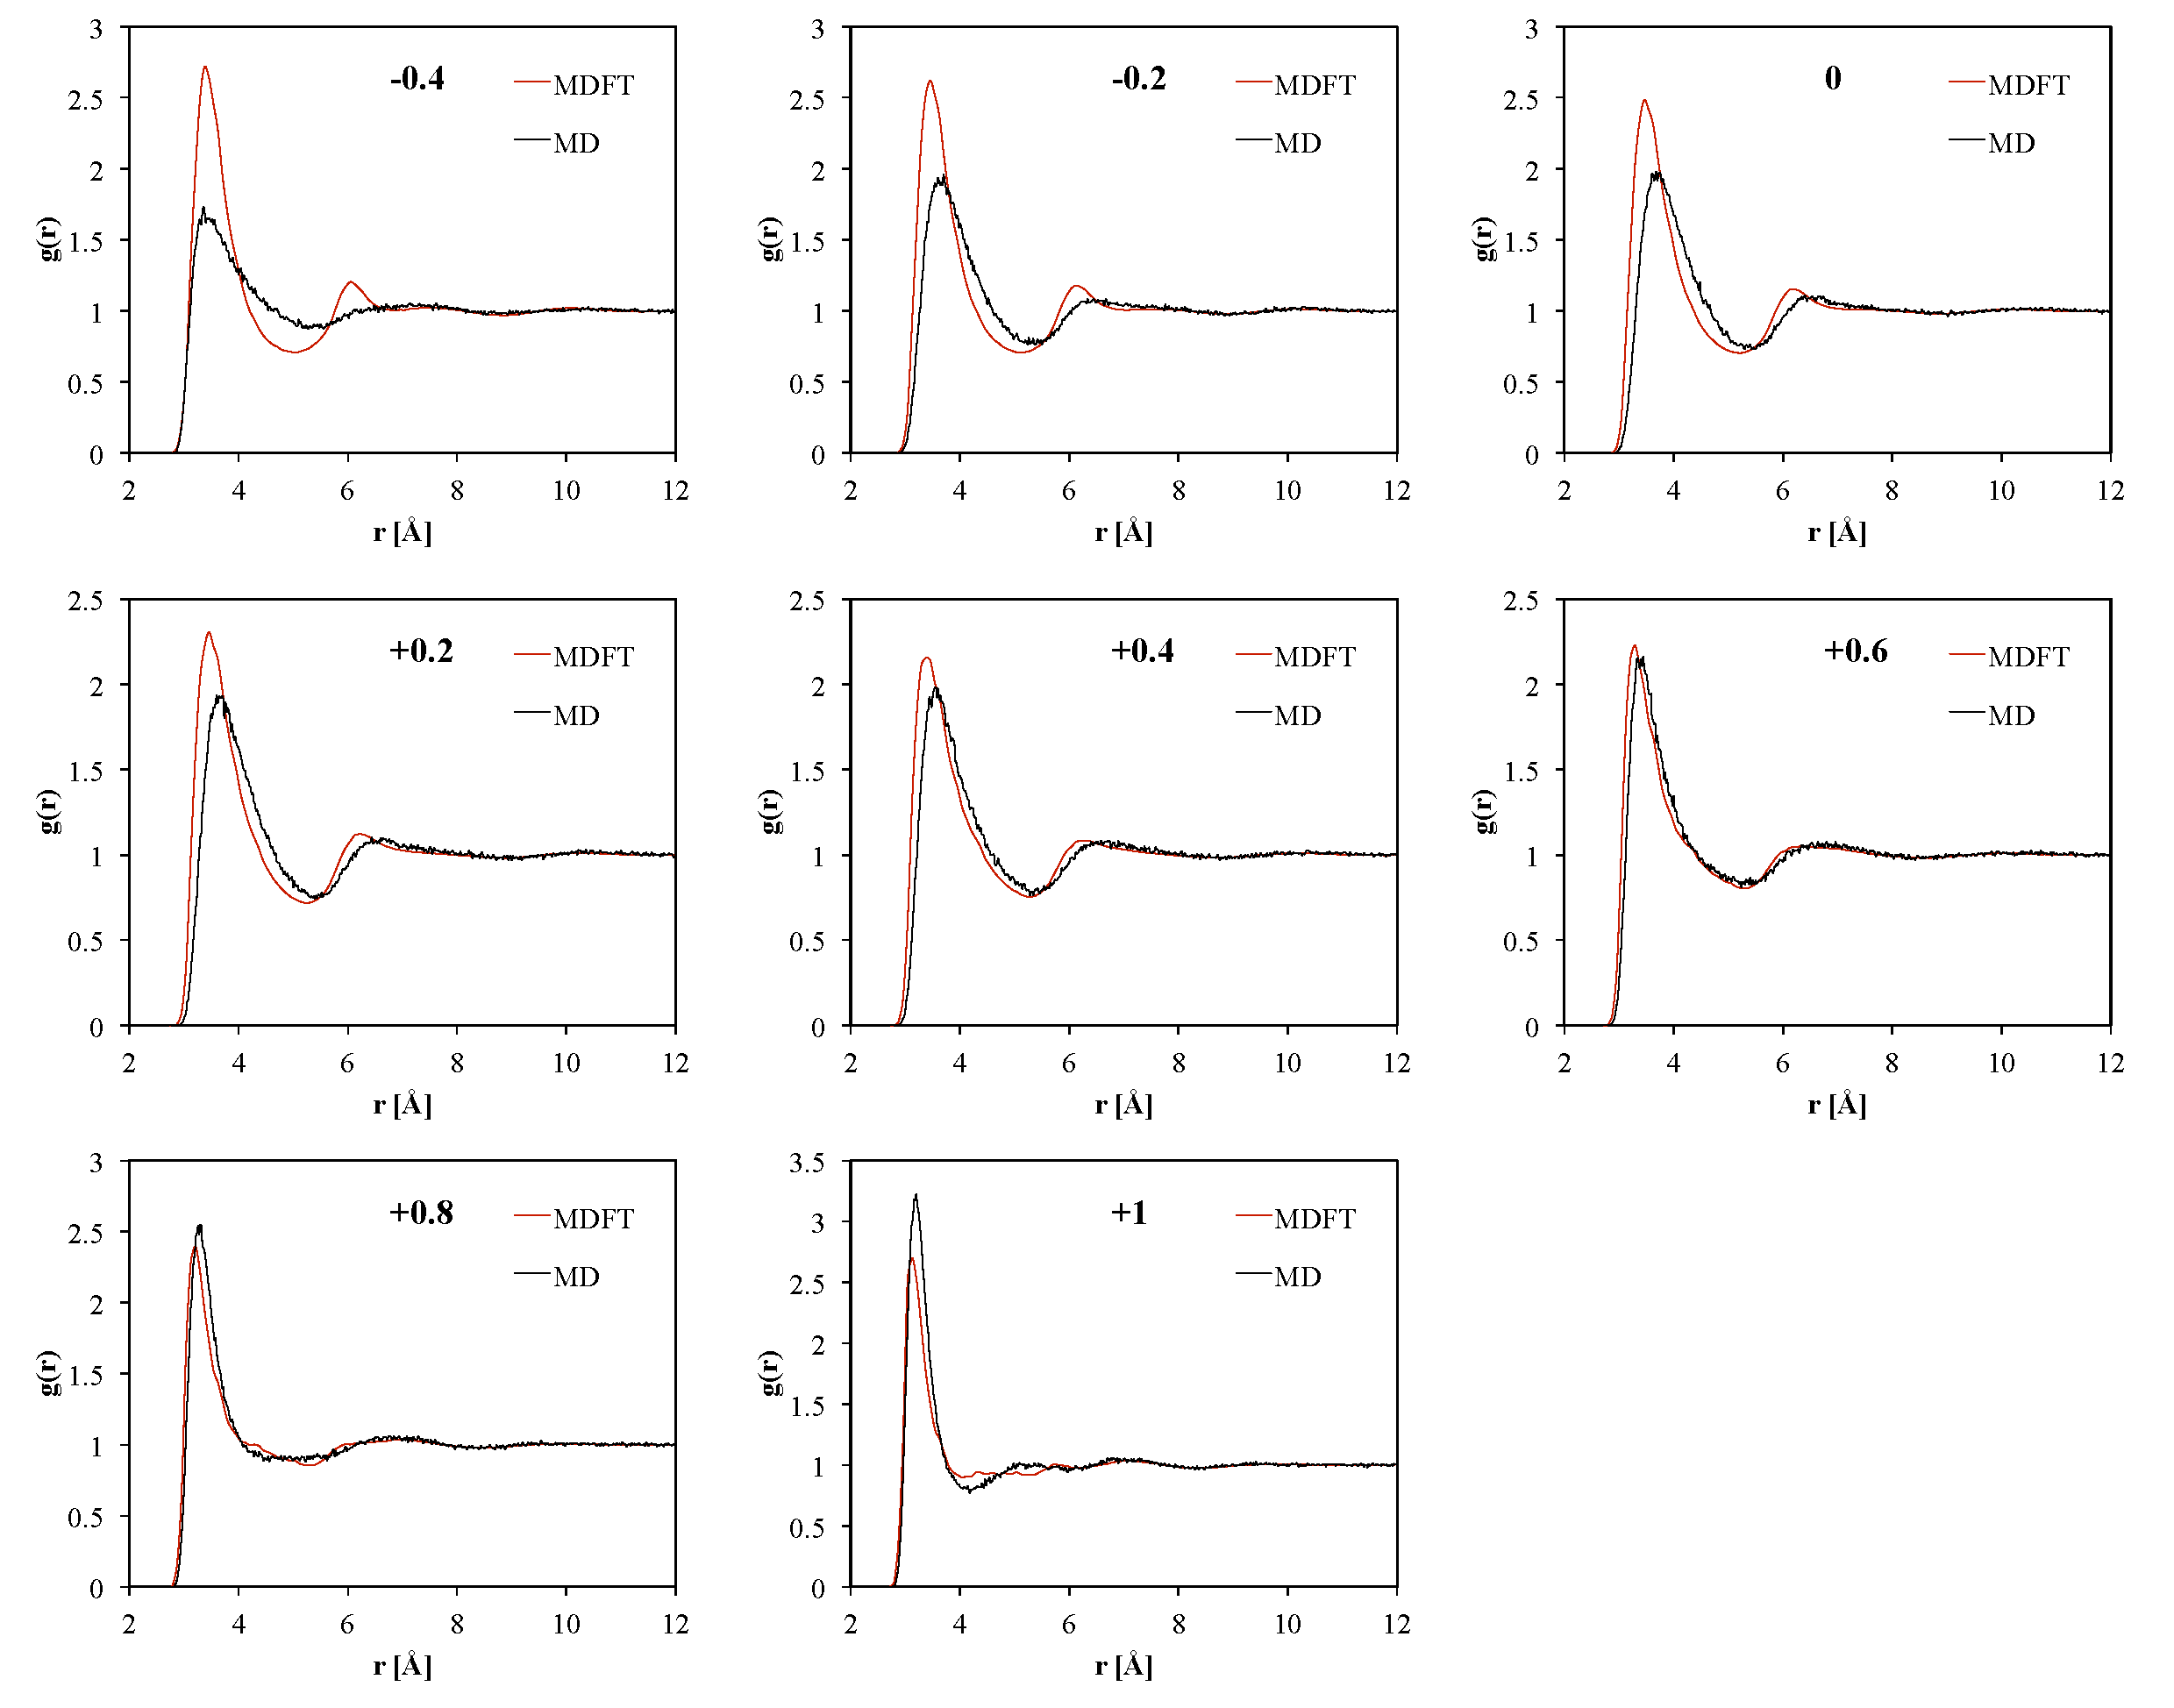
\includegraphics[width=1\columnwidth]{/Users/Hostiphre/Desktop/_M1102/_figure/results/ch4_md}
\par\end{centering}
\caption{Comparison to IET. Profile of $\rho$ in rotational invariant projections.\label{fig:Comparison-to-MD}}
\end{figure}


\section{Premier conclusion}

From the results, we see that MDFT ... ``capable'' to produce the
same result with IEM for single ions. (but have more ability to calculate
3D molecules which is not suitable for spherical coordinates...)

\texttt{\textbf{naive\_interpolation}} is more stable compared to
\texttt{\textbf{convolution}} methods and can use less angles for
convergence, although in the computing time it cannot compare with
\texttt{\textbf{convolution}} methods, which will be discussed later.

\begin{figure}[h]
\begin{centering}
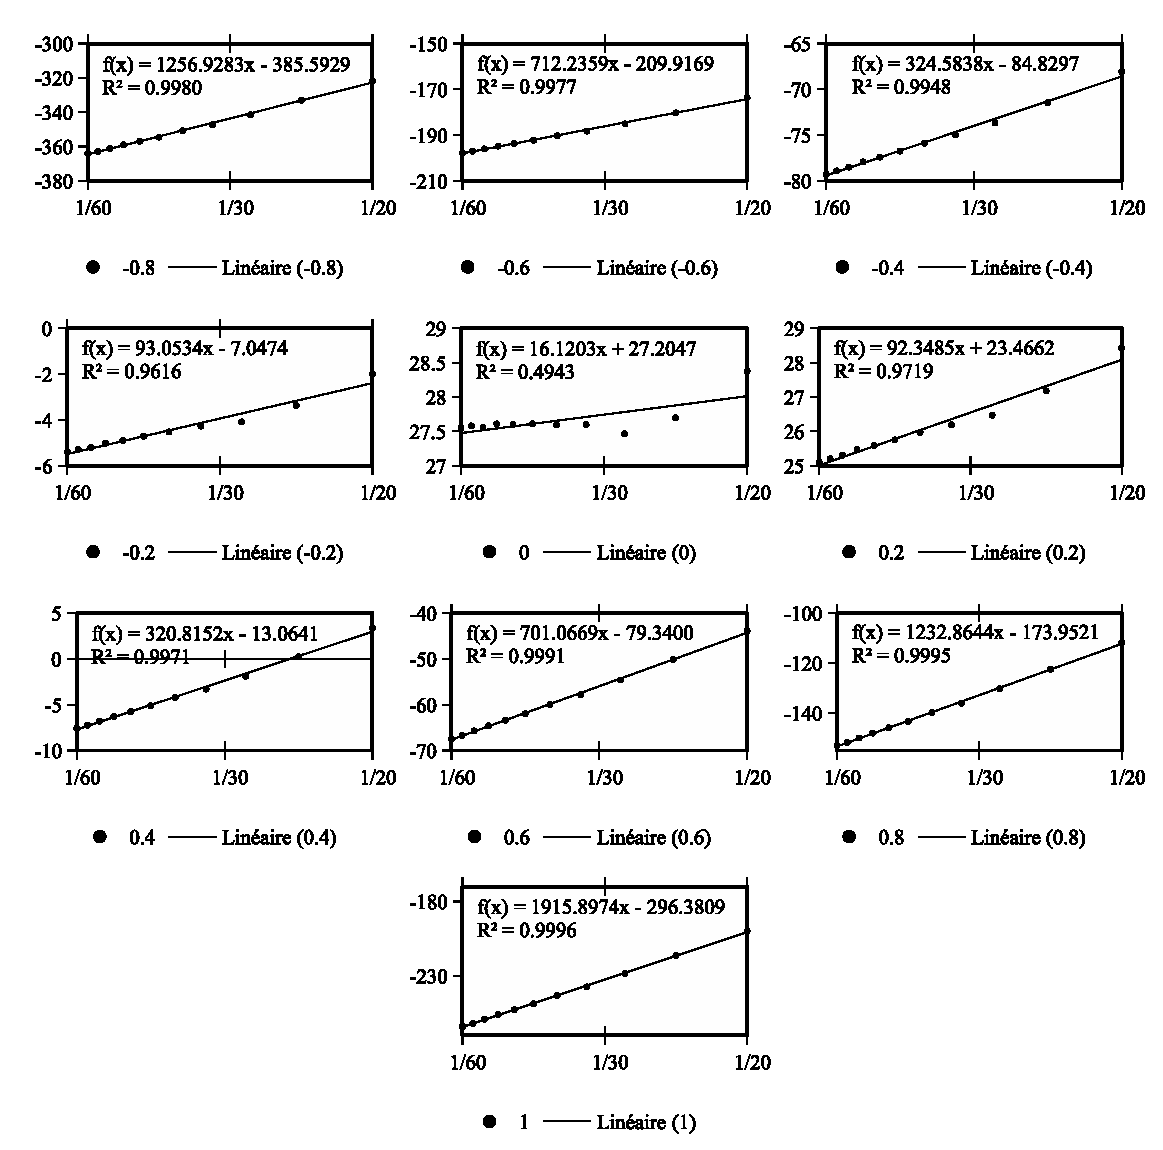
\includegraphics[width=0.95\columnwidth]{_figure/results/ch4_nmax1_lmn}
\par\end{centering}
\caption{Free energy (without correction) of charged $\mathrm{C}\mathrm{H}_{4}$
centre (-1.0 to 1.0) with respect to the box length, for \texttt{\textbf{naive\_nmax1}}
method, with $m_{\max}=n_{\max}=1$, at 300K.\label{fig:ch4_nmax1_lmn}}
\end{figure}

\begin{figure}[!th]
\begin{centering}
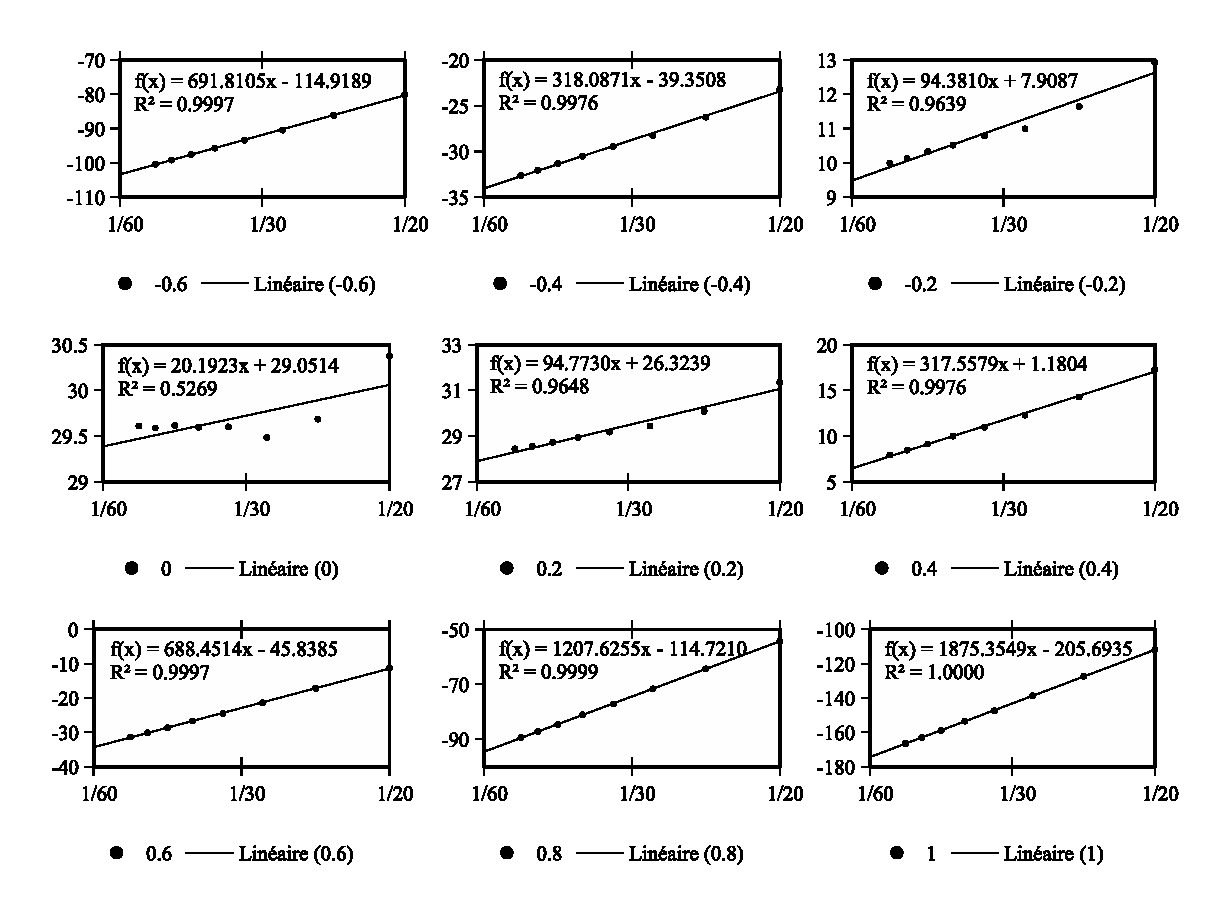
\includegraphics[width=0.95\columnwidth]{_figure/results/ch4_nmax5_inter}
\par\end{centering}
\caption{Free energy (without correction) of charged $\mathrm{C}\mathrm{H}_{4}$
centre (-1.0 to 1.0) with respect to the box length, for \texttt{\textbf{naive\_interpolation}}
method, with 14 angles of Lebedev quadrature angles for $\Theta$
and $\Phi$, 3 for $\Psi$, DCF of $n_{\max}=5$, at 300K.\label{fig:ch4_nmax5_inter}}
\end{figure}

\begin{figure}[!bh]
\begin{centering}
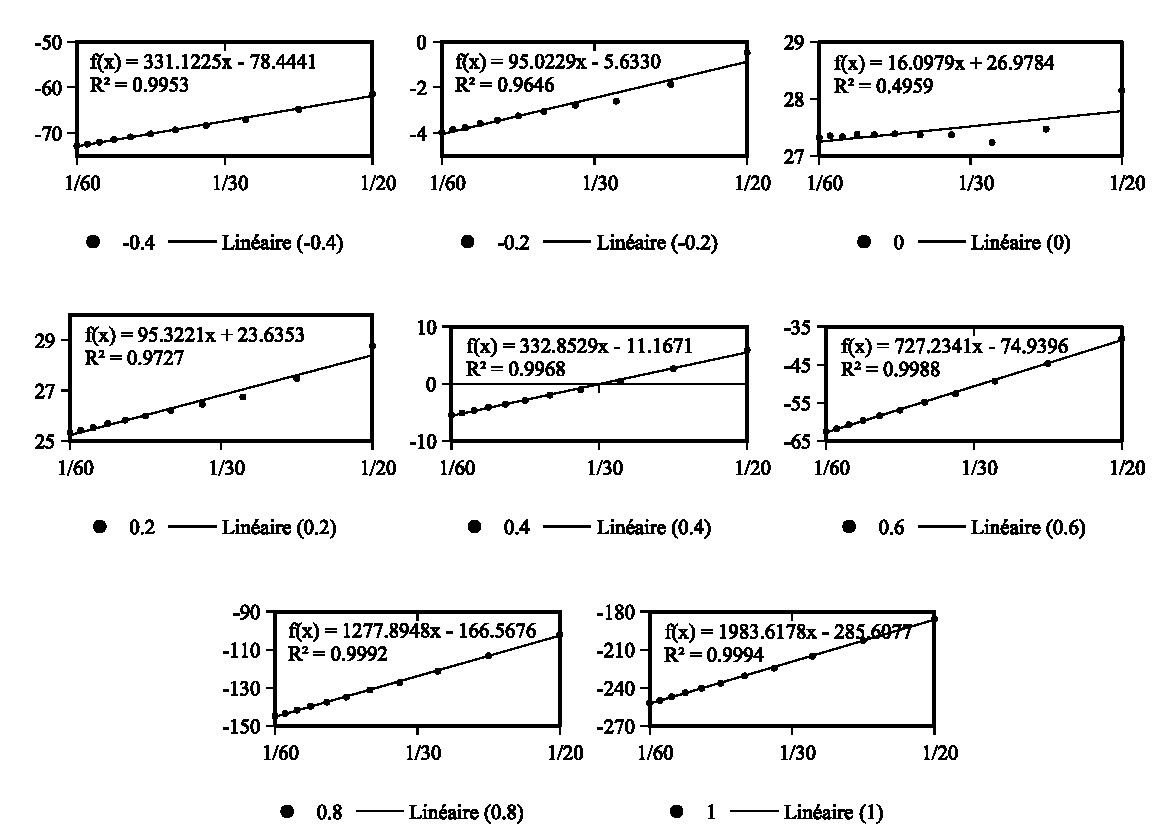
\includegraphics[width=0.95\columnwidth]{_figure/results/ch4_nmax1_new}
\par\end{centering}
\caption{Free energy (without correction) of charged $\mathrm{C}\mathrm{H}_{4}$
centre (-1.0 to 1.0) with respect to the box length, for \texttt{\textbf{convolution\_standard}}
method, with $m_{\max}=n_{\max}=1$, at 298.15K.\label{fig:ch4_nmax1_new}}
\end{figure}




\chapter{Computing Performance \label{chpt:seq-code-performance}}

This section evaluates the computing performance (timing) of the code.
Our goal is to show that the new algorithm of angular convolution
is much faster than the old naive one; the huge amount of simulation
during this thesis has proven that to be the case. But a raw result,
where the implementation goes for an indefinite number of iterations
during minimization, cannot give a proper and systematic performance
evaluation. This is the purpose of this section.

In this section, we will evaluate the performance only within the
$\mathcal{F}_{\mathrm{exc}}$ term, knowing that other two terms takes
time of the same magnitude than the new algorithms for $\mathcal{F}_{\mathrm{exc}}$
part. The spatial and angular grid dependence of branches are discussed.

\section{FFT}

The \acs{FFT} play an important role in the implementation, which
is used by the spatial convolution and the \acs{FGSHT} process. 

\begin{figure}[H]
\begin{centering}
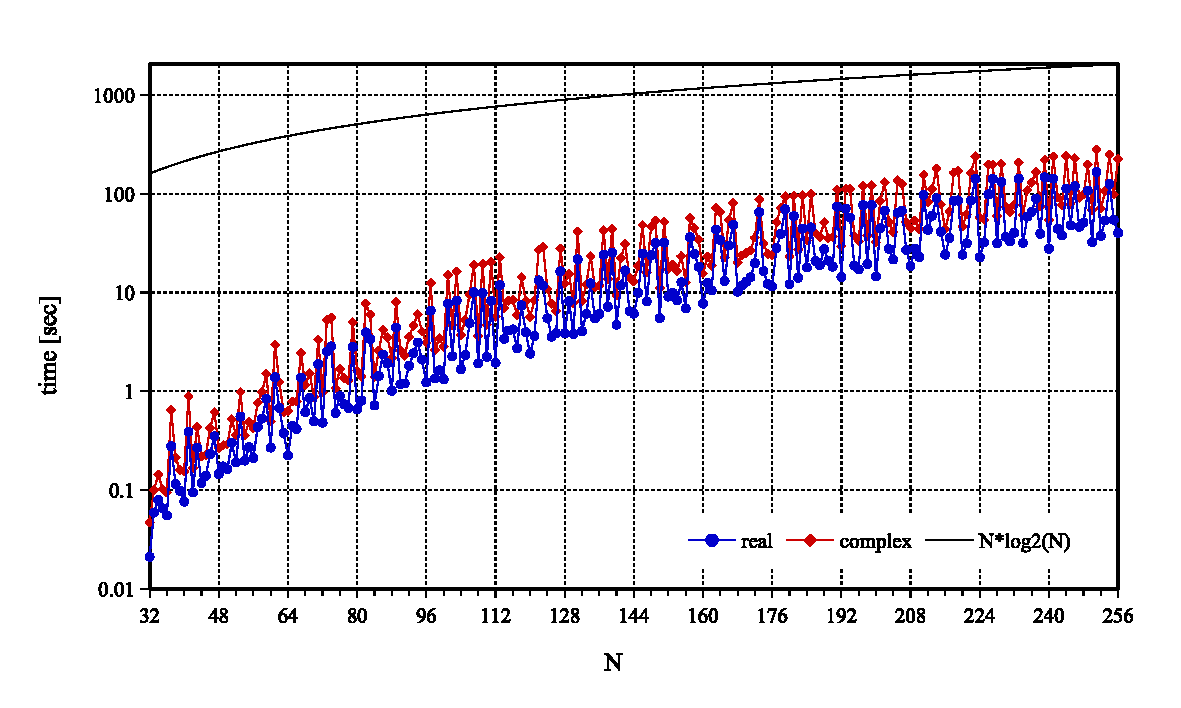
\includegraphics[bb=0bp 20bp 567bp 310bp,width=1\columnwidth]{_figure/results/fftw_timing}
\par\end{centering}
\caption{Timing of \acs{FFT} for real-to-complex and complex-to-complex processes
with respect to grid number $N$\label{fig:timing-FFT}}
\end{figure}

Referring to figure \ref{fig:timing-FFT}, the dependance on $O(N\log_{2}N)$
\citep{Numerical_Recipes_3ed} doesn't totally exist, but of the same
form, depending on the algorithm of \acs{FFT} \citep{Briggs-DFT}.
It should be noted that a grid of prime number is always at the peaks
in the figure, which means it can be 2 or more times longer than that
of the composite number around. Therefore it is better to use an even
number grid, where the $k$-border correction in $\mathsection$\ref{subsec:k-border-effect}
is absolutely involved in. Apart from this conclusion, to compare
between the algorithms for angular part involved in this thesis, we
are not really interested in computing performance with respect to
the number of spatial grid. However, the ratio of real and complex
\acs{FFT} timing is important, illustrated in figure \ref{fig:fft-real-to-complex},
where the ratio between real-to-complex and complex-to-complex \acs{FFT}
processes is 0.54, near the theoretical ratio 0.5. For example, we
process $n_{\mathrm{angle}}$ real to complex \acs{FFT}, then $n_{\mathrm{spatial}}/2$
complex to complex \acs{FGSHT}. Or we process $n_{\mathrm{spatial}}$
real to complex \acs{FGSHT}, then $n_{\mathrm{proj}}/2$ complex
to complex \acs{FFT}. This should not give a great difference if
$n_{\mathrm{angle}}\sim n_{\mathrm{proj}}$ for small $n_{\max}$.
If the the ratio is not 1:2, it will have an influence on the choice
of algorithm.
\begin{center}
\begin{figure}[h]
\begin{centering}
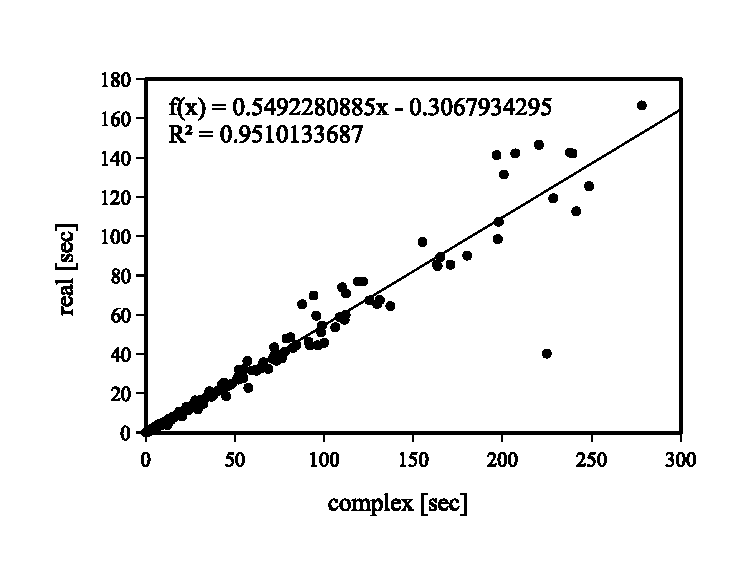
\includegraphics[bb=0bp 20bp 340bp 235bp,width=0.5\columnwidth]{_figure/results/fftw_real_v_cmplx}
\par\end{centering}
\caption{Timing of real-to-complex \acs{FFT} processes with respect to its
complex-to-complex process of the same grid number $N$\label{fig:fft-real-to-complex}}
\end{figure}
\par\end{center}

\section{FGSHT}

The computing times of \acs{GSHT} and \acs{FGSHT} are shown in figure
\ref{fig:time-gsht-fgsht}. There is no reason to see in detail how
much \acs{FFT} has accelerated the \acs{GSHT} process, but clearly
\acs{FGSHT} can be 100 times faster than \acs{GSHT}, and \acs{GSHT}
for the symmetry of $\Psi$, $s=1$ is on average 5 times longer than
$s=2$ ($s$ being the \acs{MRSO} defined in $\mathsection$\ref{sec:fgsht}).
As accuracy test shows that \acs{GSHT} and \acs{FGSHT} give exactly
the same result, and the case $m_{\max}<n_{\max}$ is never needed,
it is possible to utilize \acs{FGSHT} in all the cases to have a
faster performance.
\begin{center}
\begin{figure}[H]
\begin{centering}
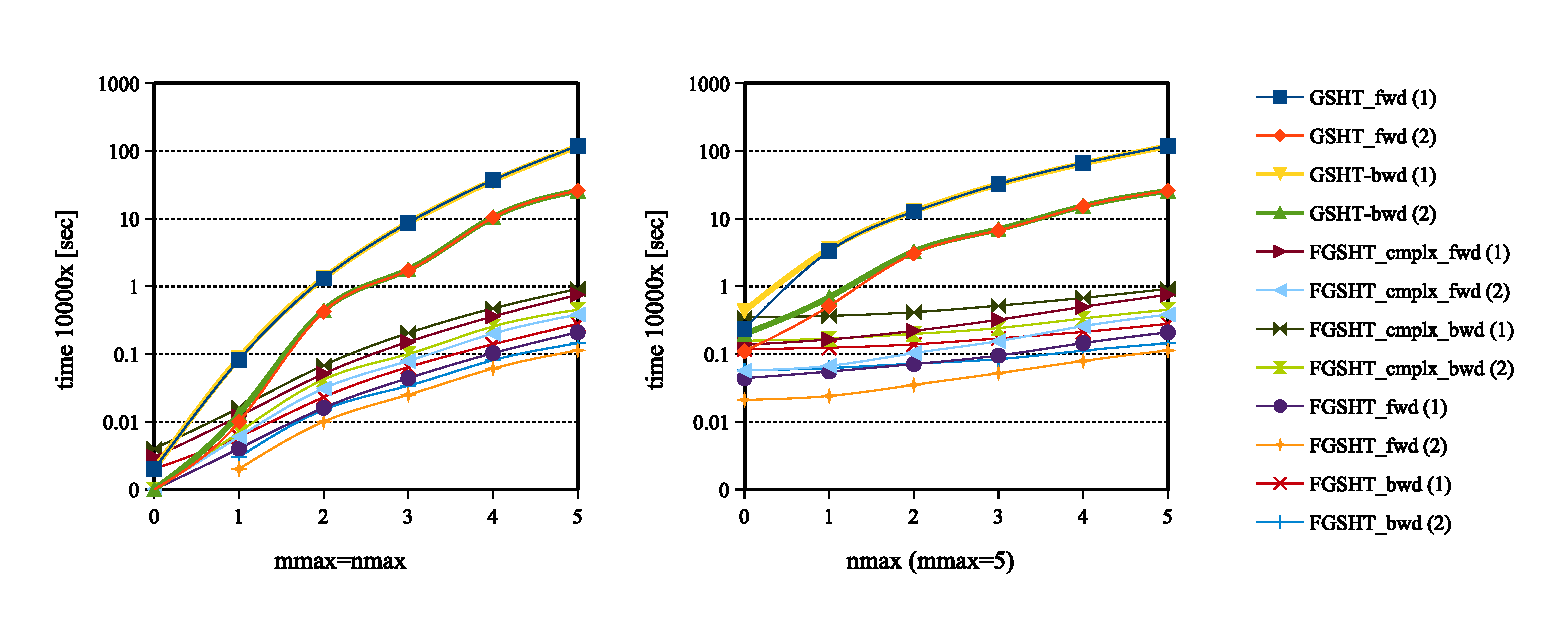
\includegraphics[bb=0bp 20bp 731bp 263bp,width=1\columnwidth]{_figure/results/fgsht_perf}
\par\end{centering}
\caption[Computing time of \acs{GSHT} and \acs{FGSHT}]{Computing time of \acs{GSHT} and \acs{FGSHT} (per 10000 times),
between parentheses is the order of symmetry axes $s$\label{fig:time-gsht-fgsht}}
\end{figure}
\par\end{center}

However, it is important to know the ratio between real and complex
\acs{FGSHT} processes for the same reason as \acs{FFT}. It is demonstrated
that this number is 0.3 in all cases, and it does not depend on $m_{\max}$,
$n_{\max}$ or $s.$ The difference between these two is that the
real one performs real-to-complex \acs{FFT} for the $\Phi,\Psi$
grid and calculates only slightly more than half of projections ($\mu\geq0$)
than the complex one.\textcolor{red}{{} }Theoretically, the ratio should
be greater than 0.5. This could mean there may be an extra process
in the complex one, or it is controlled by the memory. Ultimately,
the final result 0.3 means, that doing $n_{\mathrm{spatial}}$ real
to complex \acs{FGSHT} takes only 0.6 the time of doing $n_{\mathrm{spatial}}/2$
complex to complex \acs{FGSHT}, which means in \texttt{\textbf{convolution\_standard}}
we use less time to compute \acs{FGSHT} than in \texttt{\textbf{convolution\_pure\_angular}}.
\textcolor{red}{(Which is in fact not observed in the following tests.)}
\begin{center}
\begin{figure}[H]
\begin{centering}
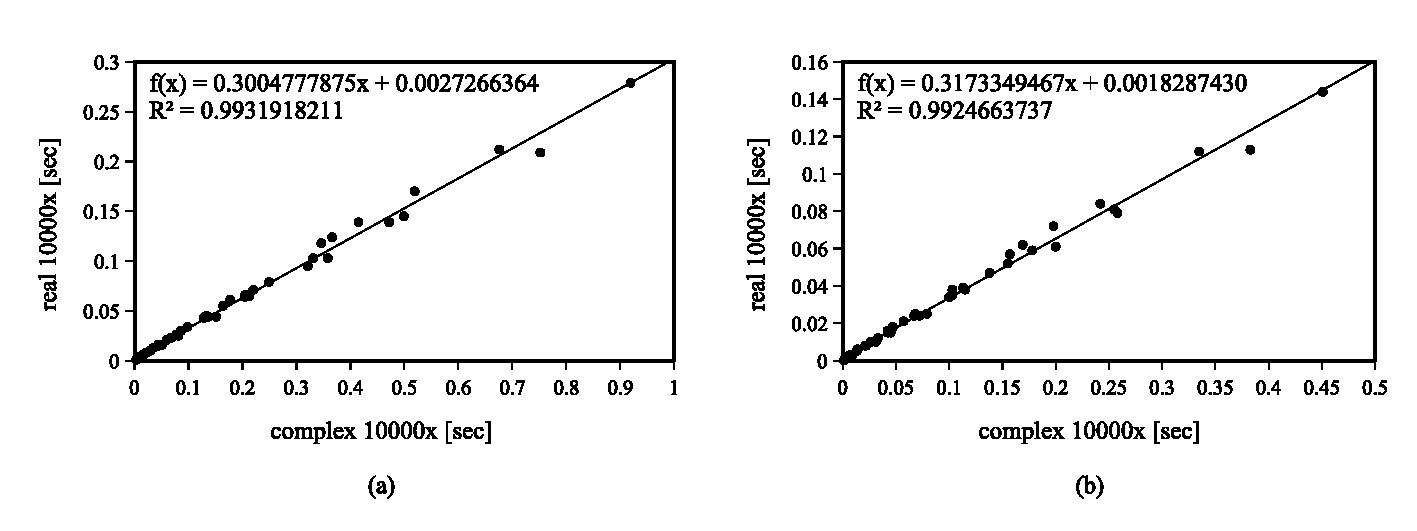
\includegraphics[bb=0bp 20bp 680bp 235bp,width=1\columnwidth]{_figure/results/fgsht_real_v_cmplx}
\par\end{centering}
\caption[Timing of real-to-complex \acs{FGSHT} processes with respect to its
complex-to-complex process of the same $m_{\max}$ and $n_{\max}$]{Timing of real-to-complex \acs{FGSHT} processes with respect to
its complex-to-complex process of the same $m_{\max}$ and $n_{\max}$,
for $s=1$ and $s=2$\label{fig:fgsht-real-to-complex}}
\end{figure}
\par\end{center}

\section{$k$-kernel\label{sec:-kernel}}

As discussed in the previous section, the final result of energy and
structure is independent of the choice of path inside a $k$-kernel.
That means we are free in terms of precision cost to choose the fast
path. Path (1) passed directly by $\hat{c}(k,\mathbf{\Omega}_{1},\mathbf{\Omega}_{2})$
in figure \ref{fig:k-kernel} has no interest in timing, as the memory
limit does not support such a direct algorithm for the entire $k$-space.
Here we only compare the paths (2), (3) and (4), which correspond
to eq. (\ref{eq:gamma-k}), (\ref{eq:im}) and (\ref{eq:gamma-blum}).

The theoretical predictions of the computing time of \acs{OZ} equation
with respect to $m_{\max}=n_{\max}$ are listed in table \ref{tab:FE-of-OZ}.
If the \acs{OZ} equation is the most time-consuming part, the result
should have the same proposal. Figure \ref{fig:Timing-k-kernel} shows
the experimental timing of the three paths, where path (3) is 100
times longer than (4), well corresponding to the theoretical value.
Path (2) is much longer than path (3) because apart from the \acs{OZ}
equation, the lecture and calculation of the \acs{DCF} mentioned
in $\mathsection$\ref{chpt:fft-spatial} also takes time.

\begin{figure}[H]
\begin{centering}
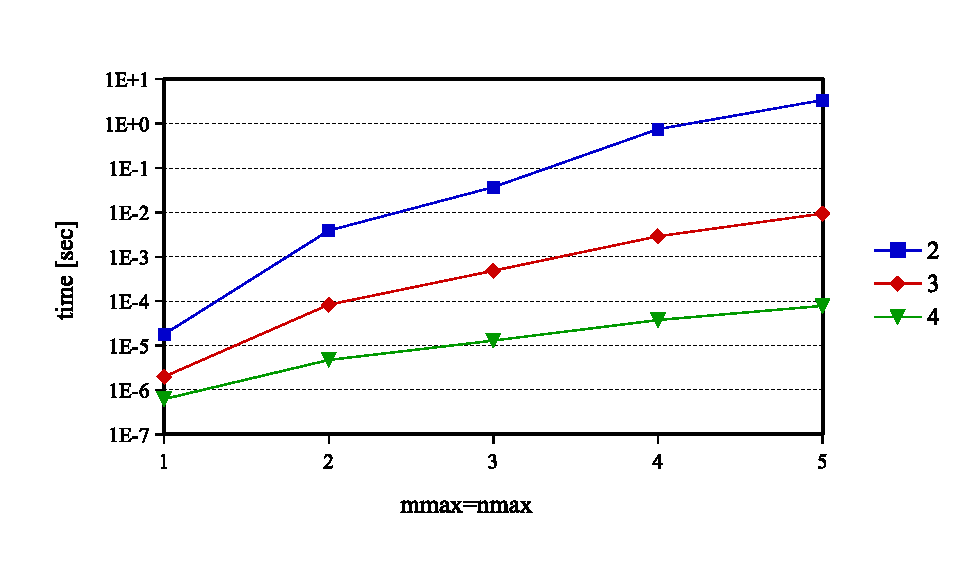
\includegraphics[bb=0bp 20bp 453bp 236bp,width=0.7\columnwidth]{_figure/results/k-kernel}
\par\end{centering}
\caption[Timing of a $k$-kernel]{Timing of a $k$-kernel (log scale)\label{fig:Timing-k-kernel}}
\end{figure}


\section{Entire iteration of $\mathcal{F}_{\mathrm{exc}}$ evaluation}

Apart from all the \texttt{\textbf{naive}} methods that will be discussed
in $\mathsection$\ref{subsec:Comparison-between-naive_standar},
figure \ref{fig:Entire-iteration} shows all the comparable \texttt{\textbf{convolution}}
timing data. We can see \texttt{\textbf{convolution\_standard}} is
the fastest algorithm, and \acs{OZ} equation is not the longest part
in the iteration. All the tests are performed for a $L=24$, $\mathrm{nfft}=72$
grid with 4 series: the three \texttt{\textbf{convolution}} methods
with $m_{\max}=n_{\max}$, and \texttt{\textbf{convolution\_standard}}
with $m_{\max}=5$, varying $n_{\max}$.

\begin{figure}[H]
\begin{centering}
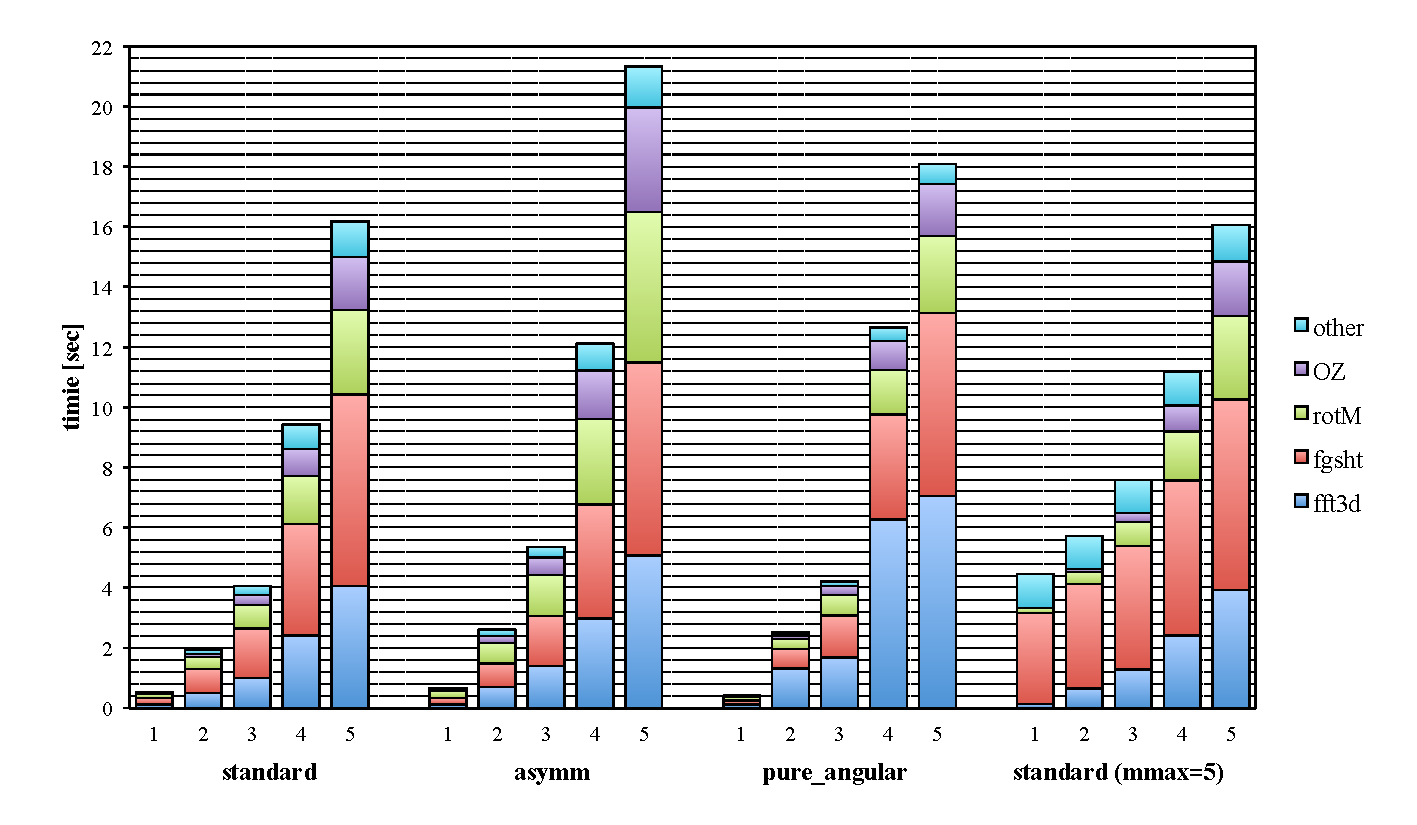
\includegraphics[width=0.9\columnwidth]{_figure/results/branch_perf}
\par\end{centering}
\caption[Entire iteration of $\mathcal{F}_{\mathrm{exc}}$ evaluation]{Entire iteration of $\mathcal{F}_{\mathrm{exc}}$ evaluation: timing
overall / decomposition of timing for 1 iteration evaluation\label{fig:Entire-iteration}}
\end{figure}


\subsection{``naive'' methods and ``convolution\_pure\_angular''\label{subsec:Comparison-between-naive_standar}}

The \texttt{\textbf{naive\_standard}}, \texttt{\textbf{naive\_interpolation}},
and \texttt{\textbf{convolution\_pure\_angular}} methods share the
same processes out of the $k$-kernel. Table \ref{tab:Timing-loop-k}
shows the timing of loop $k$ of these three methods. It indicates
that \texttt{\textbf{convolution\_pure\_angular}} takes far less time
than the other two methods, of which the loop $k$ takes time in the
same order of magnitude as the rest of iteration. And once $m_{\max}\geq2$,
\texttt{\textbf{naive\_interpolation}} is faster than \texttt{\textbf{naive\_standard}}.
Note that order 2 of \texttt{\textbf{naive\_interpolation}} can give
good results for a \acs{DCF} of $n_{\max}=5$. So in every case of
\texttt{\textbf{naive}} methods, \texttt{\textbf{naive\_interpolation}}
should be used. This verifies the conclusion of $k$-kernel test in
that the path (4) in figure \ref{fig:k-kernel} is the fastest.

\begin{table}[H]
\begin{centering}
\begin{tabular}{ccccc}
\toprule 
$m_{\max}$ & \texttt{\textbf{naive\_standard}} & \texttt{\textbf{naive\_interpolation}} & \texttt{\textbf{convo\_pure\_angular}} & \tableheadline{Other}\tabularnewline
\midrule
1 & 2.34 & 4.42 & 0.26 & 0.15\tabularnewline
2 & 365.95 & 209.12 & 1.09 & 1.43\tabularnewline
3 & 3295.00 & 752.70 & 2.37 & 1.85\tabularnewline
4 & too long & too long & 5.93 & 6.73\tabularnewline
5 & too long & too long & 10.36 & 7.73\tabularnewline
\bottomrule
\end{tabular}
\par\end{centering}
\caption[Timing of loop $k$]{Timing {[}sec{]} of loop $k$ of ``naive\_standard'', ``naive\_interpolation''
and ``convolution\_pure\_angular'', and the rest of iteration\label{tab:Timing-loop-k}}
\end{table}


\subsection{``convolution\_standard'' and ``convolution\_pure\_angular''}

The comparison of \texttt{\textbf{convolution\_standard}} and \texttt{\textbf{convolution\_pure\_angular}}
appears in figure \ref{fig:comparison-pure_angular}. Their difference
lies in the inversion of \acs{FFT} and \acs{FGSHT}. We can see the
other parts are almost identical, but the implementation of \acs{FFT}
is different in terms of time. Because in \texttt{\textbf{convolution\_standard}}
the number of \acs{FE} we need for \acs{FFT} is the number of projections,
and in \texttt{\textbf{convolution\_pure\_angular}} it is the number
of angular grid nodes. As there are fewer projections than angular
nodes, \texttt{\textbf{convolution\_standard}} reasonably takes less
time. The stair form of the \texttt{\textbf{pure\_angular}} curve
is due to the grid $\Psi$, which takes $\left\lfloor m_{\max}/2\right\rfloor $
points in the presence of $\mathrm{C}_{2v}$ symmetry. Projections
are less sensible.

\begin{figure}[H]
\begin{centering}
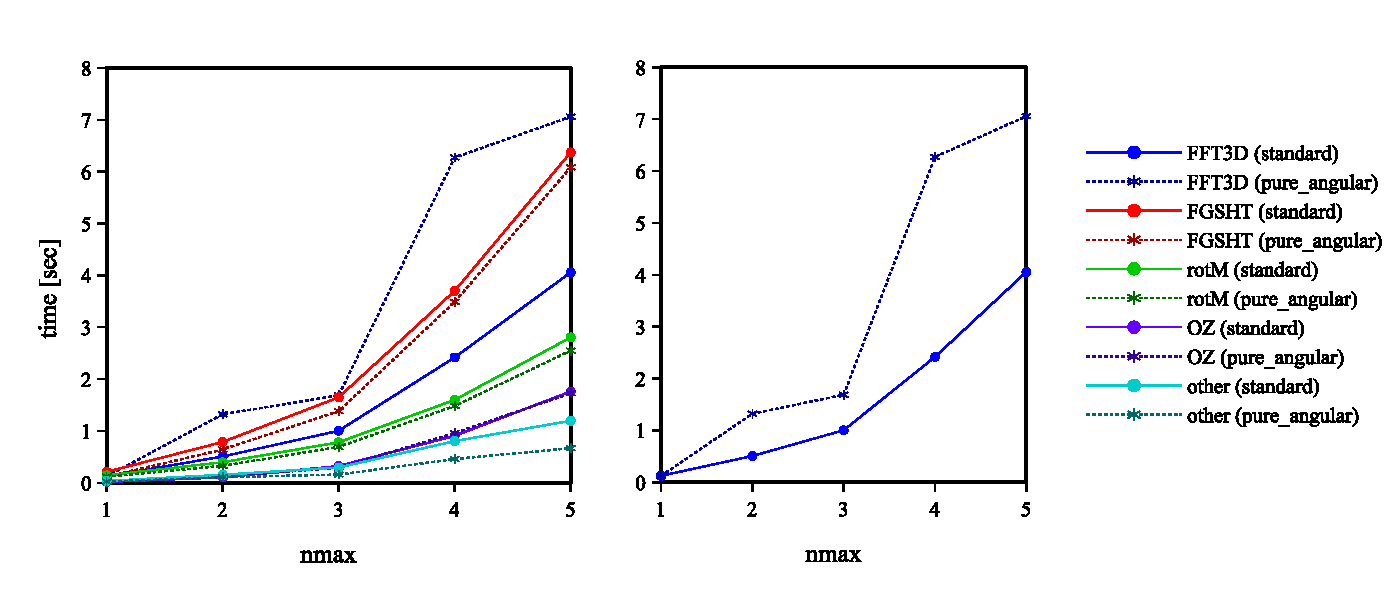
\includegraphics[bb=0bp 20bp 667bp 268bp,width=1\columnwidth]{_figure/results/pure_angular}
\par\end{centering}
\caption[Performance comparison of ``convolution\_standard'' and ``convolution\_pure\_angular'']{Performance comparison of \texttt{\textbf{convolution\_standard}}
and \texttt{\textbf{convolution\_pure\_angular\label{fig:comparison-pure_angular}}}}
\end{figure}


\subsection{``convolution\_standard'' and ``convolution\_asymm''}

We compare\texttt{\textbf{ convolution\_standard}} and \texttt{\textbf{convolution\_asymm}}
in figure \ref{fig:comparison-asymm}. The difference is that \texttt{\textbf{standard}}
calculates a half $k$ in the $k$-loop and \texttt{\textbf{asymm}}
calculates all $k$ in the $k$-loop. They share the same process
of \acs{FGSHT}; for the processes in a $k$-loop (rotM, OZ) \texttt{\textbf{asymm}}
always takes longer time. As in \texttt{\textbf{asymm}} we calculate
the \acs{FFT} for all the projections and in \texttt{\textbf{standard}}
we calculate only a half projections with $\mu\geq0$, the time consumed
by \acs{FFT} is also different.

\begin{figure}[H]
\begin{centering}
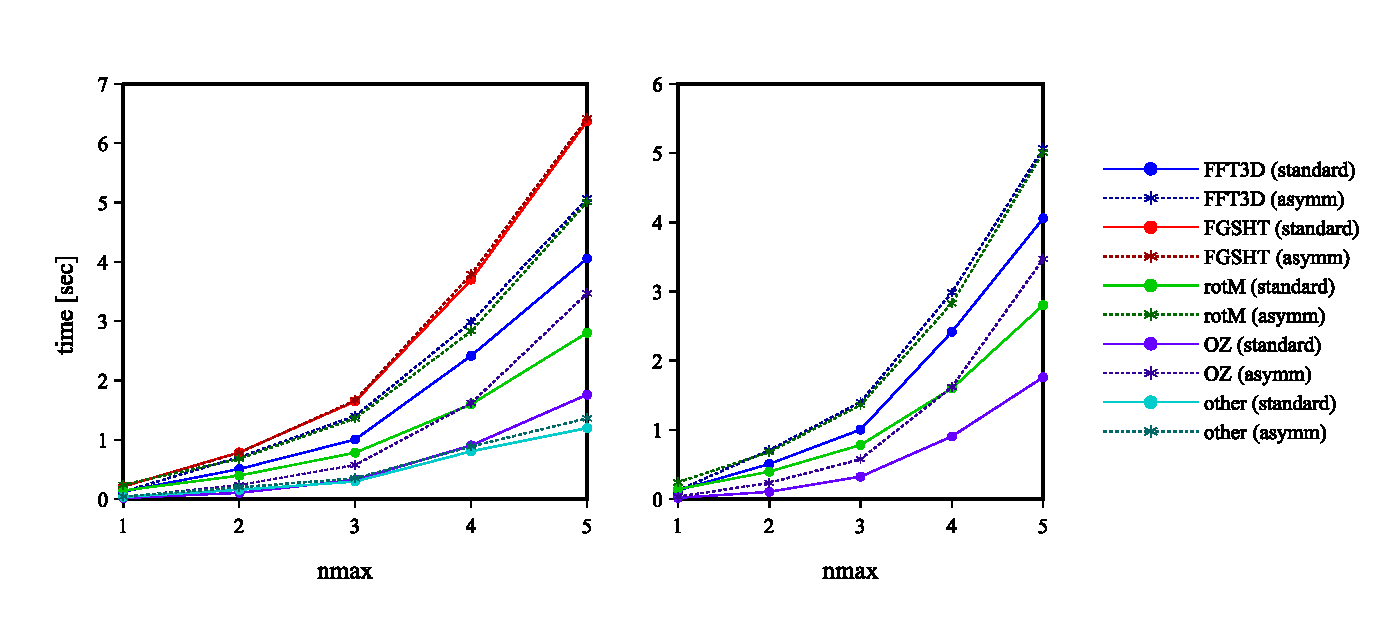
\includegraphics[bb=0bp 20bp 648bp 268bp,width=1\columnwidth]{_figure/results/asymm}
\par\end{centering}
\caption[Performance comparison of ``convolution\_standard'' and ``convolution\_asymm'']{Performance comparison of \texttt{\textbf{convolution\_standard}}
and \texttt{\textbf{convolution\_asymm\label{fig:comparison-asymm}}}}
\end{figure}


\subsection{Distinction of $m_{\max}$ and $n_{\max}$}

The comparison of $m_{\max}=n_{\max}$ and $m_{\max}=5$ for\texttt{\textbf{
convolution\_standard}} is shown in figure \ref{fig:comparison-nmax}.
We see that the choice of quadrature order $m_{\max}$ only affects
the \acs{FGSHT} process and the lecture/storage of density variable
(other). The time taken by extra order $m_{\max}$ is not cost-free,
as discussed in last section, it is fully recommended to use $m_{\max}=n_{\max}$.

\begin{figure}[H]
\begin{centering}
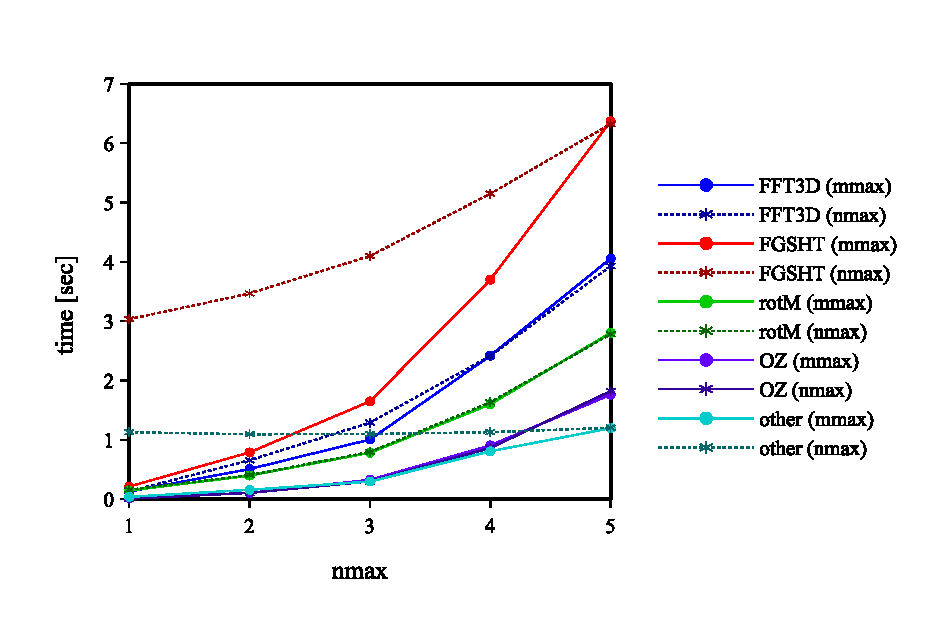
\includegraphics[bb=0bp 20bp 639bp 268bp,width=1\columnwidth]{_figure/results/nmax}
\par\end{centering}
\caption[Performance comparison of ``convolution\_standard'' for $m_{\max}=n_{\max}$
and $m_{\max}=5$]{Performance comparison of \texttt{\textbf{convolution\_standard}}
for $m_{\max}=n_{\max}$ and $m_{\max}=5$\label{fig:comparison-nmax}}
\end{figure}


\section{Global view of the code performance}

\begin{figure}[H]
\begin{centering}
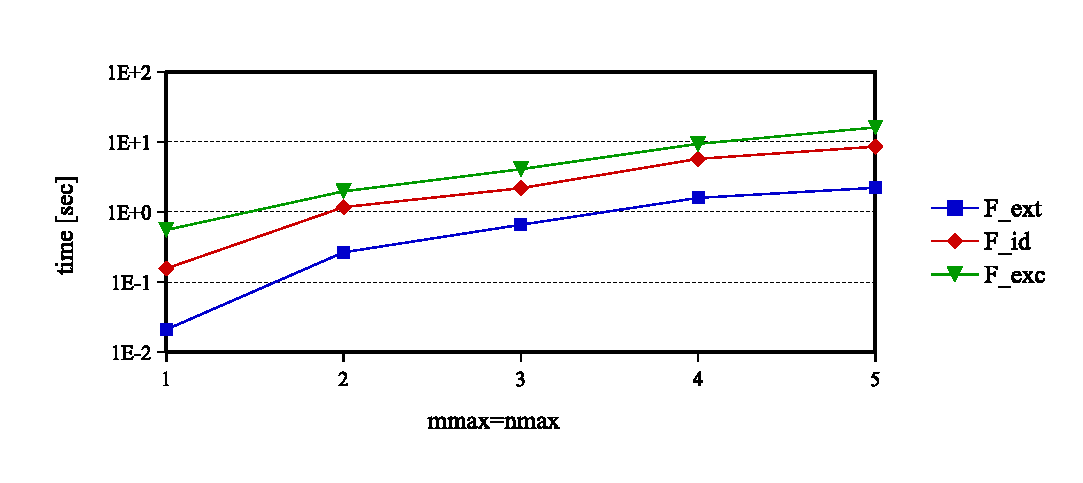
\includegraphics[bb=0bp 20bp 453bp 236bp,scale=0.7]{_figure/results/global_perf}
\par\end{centering}
\caption[Timing of the whole $\mathcal{F}$ iteration]{Timing of the whole $\mathcal{F}$ iteration with $\mathrm{nfft}/L=72/24$
grid (log scale)}
\end{figure}

We can see that \texttt{\textbf{convolution\_standard}} is the fastest.
The \texttt{\textbf{convolution}} methods are orders of magnitude
faster than \texttt{\textbf{naive}} methods. The evaluation of $\mathcal{F}_{\mathrm{exc}}$
is at the same order of magnitude than other two terms and the same
dependency on angular grid.



\chapter{Computing performance of parallel code\label{chpt:parallelization}}


\section{Node-level Parallelization}

OpenMP, scalability with respect to the number of thread


\section{Parallelization on Several Nodes}

MPI, scalability with respect to the number of node


\ctparttext{Only a few applications are made due to the time limit of this thesis,
concluding\\
\medskip{}
Section {[}ref{]} to show the capability of MDFT to calculate ions
and small molecules.\\
\medskip{}
Section {[}ref{]} to show a qualitative influence of polar solvent
on the reaction including metal-oxo centre.}

\part{Applications}


\chapter{Comparison to MD simulation\label{chpt:ions}}

In the last chapter, we have proven that \acs{MDFT} is capable to
correctly predict solvation properties of LJ centers, single ions
and linear solutes compared to \acs{IET}. In this section, we will
compare them to \acs{MD} and experimental results. All the solutes
are optimized with the fast \texttt{\textbf{convolution\_standard}}
algorithm, with implicitly $L=24$ $\textrm{Å}$, $\mathrm{nfft}=72$,
$m_{\max}=n_{\max}$ unless otherwise specified. Comparison to the
dipole method is also involved, as we should justify that the increase
of computing cost when going from $n_{\max}=1$ to $n_{\max}>1$ is
counter-balanced by the capability to produce better results. 

\section{LJ centers}

The \acs{RDF}s of rare gases calculated in $\mathsection$\ref{tab:Free-energy-rare-gas}
are compared to \acs{MD} in figure \ref{fig:rare-gazz} using $n_{\max}=3$
to 5. The structures of different $n_{\max}$ is almost identical.
Comparing to \acs{MD}, it looks like there is no improvement compared
to the dipole method in ref \citep{Zhao_2011} or to calculation involving
$c_{00}^{000}$ only \citep{levesque_scalar_2012}. This kind of disagreement
in curve shape is regarded as a known default of \acs{HNC} (or \acs{HRF})
approximation.

\begin{figure}[h]
\begin{centering}
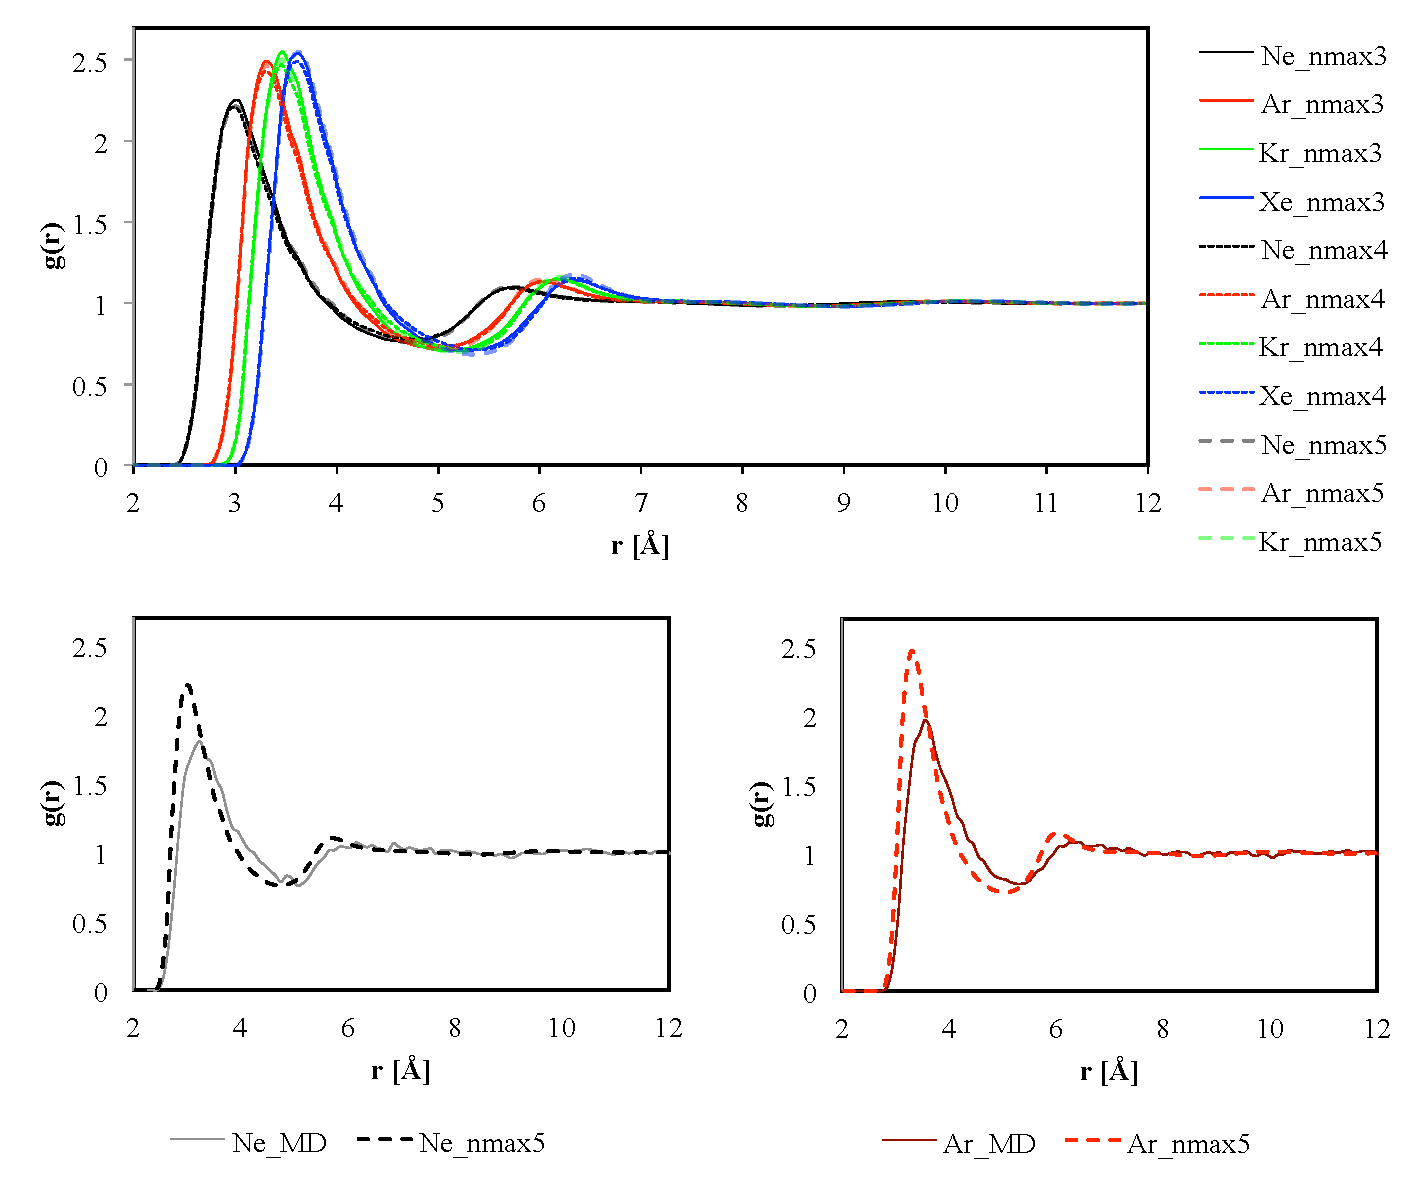
\includegraphics[width=0.95\columnwidth]{_figure/results/rare_gaz}
\par\end{centering}
\caption{\acs{RDF} of rare gazes compared to \acs{MD} result\label{fig:rare-gazz}}
\end{figure}


\section{Charged $\mathrm{CH_{4}}$ series}

The comparison between the \acs{RDF}s obtained from \acs{MDFT} with
\acs{MD} results for charged $\mathrm{CH_{4}}$ series are shown
in figure \ref{fig:Comparison-to-MD}. We can see that for positive
charges, the complete $n_{\max}=5$ gives much better results compared
to the dipole method, which itself almost agrees with \acs{MD} results.
For negative charges, $n_{\max}=5$ gives nearly the same result as
dipole method, while the \acs{MD} results are more smooth, but the
first peak of the \acs{MDFT} results seems to be in good position.
We can conclude that the complete \acs{DCF} gives a large improvement
for positive charged ions.

\begin{figure}[h]
\begin{centering}
\includegraphics[width=1\columnwidth]{_figure/results/ch4_md}
\par\end{centering}
\caption{\acs{RDF} of charged $\mathrm{CH_{4}}$ series compared to \acs{MD}
result\label{fig:Comparison-to-MD}}
\end{figure}


\section{Solvation free energy of single ions}

\marginpar{We consider that in a macroscopic system, the fluctuation of $N$
and $V$ are negligible, and all kinds of free energies becomes the
same. \citep{ensemble_thermo}}From above we can see the \acs{RDF} for positive ions are in good
agreement with \acs{MD} results. However, the free energy is more
difficult to compare, as there are several finite-size corrections
for single ions, depending on for example box length and charge; besides
the free energy depends largely on the input LJ parameters of the
ions, which is independent to the method.

Table \ref{tab:single-ions} gives from literatures some experimental
and \acs{MD} simulation results of solvation free energy as well
as the positions of the first maximum of the \acs{RDF} for alkali
and halide ions. We can see that the experimental data themselves
vary a lot. Furthermore the LJ parameters for ions in the literature
are extremely dispersed. Therefore, we focused on a single series
of force field parameters for halide anions and alkali cations taken
from ref \citep{horinek_rational_2009} based on SPC/E water, as shown
also in table \ref{tab:single-ions}. 

\begin{table}[h]
\begin{centering}
\begin{tabular*}{1\linewidth}{@{\extracolsep{\fill}}ccccccccc}
\toprule 
\addlinespace[-0.17em]
\tableheadline{{\footnotesize{}Ion}} & {\scriptsize{}$-\Delta G_{\mathrm{solv}}^{\mathrm{exp}}$\textsuperscript{{\scriptsize{}(a)}}} & {\scriptsize{}$-\Delta F_{\mathrm{solv}}^{\mathrm{exp}}$\textsuperscript{{\scriptsize{}(b)}}} & {\scriptsize{}$-\Delta G_{\mathrm{solv}}^{\mathrm{exp}}$\textsuperscript{{\scriptsize{}(c)}}} & {\scriptsize{}$R_{1}$\textsuperscript{{\scriptsize{}(d)}}} & {\scriptsize{}$\sigma$ $[\textrm{Å}]$\textsuperscript{{\scriptsize{}(e)}}} & {\scriptsize{}$\epsilon$ {[}$\mathrm{kJ\cdot mol^{-1}}${]}\textsuperscript{{\scriptsize{}(e)}}} & {\scriptsize{}$-\Delta G_{\mathrm{solv}}^{\mathrm{MD}}$\textsuperscript{{\scriptsize{}(e)}}} & {\scriptsize{}$R_{1}^{\mathrm{MD}}$\textsuperscript{{\scriptsize{}(e)}}}\tabularnewline
\midrule 
\addlinespace[-0.33em]
{\scriptsize{}$\mathrm{F^{-}}$} & {\scriptsize{}465} & {\scriptsize{}374.5} & {\scriptsize{}428.8} & {\scriptsize{}2.08} & {\scriptsize{}3.30} & {\scriptsize{}0.55} & {\scriptsize{}-430} & {\scriptsize{}2.74}\tabularnewline
\addlinespace[-0.33em]
{\scriptsize{}$\mathrm{Cl^{-}}$} & {\scriptsize{}340} & {\scriptsize{}318.4} & {\scriptsize{}304.2} & {\scriptsize{}2.36} & {\scriptsize{}3.78} & {\scriptsize{}0.52} & {\scriptsize{}-306} & {\scriptsize{}3.23}\tabularnewline
\addlinespace[-0.33em]
{\scriptsize{}$\mathrm{Br^{-}}$} & {\scriptsize{}315} & {\scriptsize{}289.5} & {\scriptsize{}227.4} & {\scriptsize{}2.80} & {\scriptsize{}4.00} & {\scriptsize{}0.37} & {\scriptsize{}-279} & {\scriptsize{}3.35}\tabularnewline
\addlinespace[-0.33em]
{\scriptsize{}$\mathrm{I^{-}}$ } & {\scriptsize{}275} & {\scriptsize{}252.3} & {\scriptsize{}240.0} & {\scriptsize{}2.89} & {\scriptsize{}4.25} & {\scriptsize{}0.32} & {\scriptsize{}-241} & {\scriptsize{}3.55}\tabularnewline
\addlinespace[-0.33em]
{\scriptsize{}$\mathrm{Li^{+}}$ } & {\scriptsize{}475} & {\scriptsize{}511.0} & {\scriptsize{}529.4} & {\scriptsize{}3.14} & {\scriptsize{}3.02} & {\scriptsize{}0.02} & {\scriptsize{}-520} & {\scriptsize{}1.91}\tabularnewline
\addlinespace[-0.33em]
{\scriptsize{}$\mathrm{Na^{+}}$ } & {\scriptsize{}365} & {\scriptsize{}411.5} & {\scriptsize{}423.8} & {\scriptsize{}2.63} & {\scriptsize{}3.49} & {\scriptsize{}0.02} & {\scriptsize{}-414} & {\scriptsize{}2.28}\tabularnewline
\addlinespace[-0.33em]
{\scriptsize{}$\mathrm{K^{+}}$ } & {\scriptsize{}295} & {\scriptsize{}337.2} & {\scriptsize{}352.0} & {\scriptsize{}3.19} & {\scriptsize{}3.85} & {\scriptsize{}0.02} & {\scriptsize{}-347} & {\scriptsize{}2.54}\tabularnewline
\addlinespace[-0.33em]
{\scriptsize{}$\mathrm{Rb^{+}}$ } & {\scriptsize{}275} & {\scriptsize{}316.0} & {\scriptsize{}329.3} & {\scriptsize{}3.37} & {\scriptsize{}no data} & {\scriptsize{}no data} & {\scriptsize{}no data} & {\scriptsize{}no data}\tabularnewline
\addlinespace[-0.33em]
{\scriptsize{}$\mathrm{Cs^{+}}$ } & {\scriptsize{}250} & {\scriptsize{}283.8} & {\scriptsize{}no data} & {\scriptsize{}3.65} & {\scriptsize{}4.17} & {\scriptsize{}0.02} & {\scriptsize{}-300} & {\scriptsize{}2.79}\tabularnewline
\bottomrule
\end{tabular*}
\par\end{centering}
\caption[Free energy and first maximum of ion-water oxygen \acs{RDF} for alkali
and halide ions from experimental and \acs{MD} simulation results]{Free energy $[\mathrm{kJ\cdot mol^{-1}}]$ and first maximum of ion-water
oxygen \acs{RDF} $[\textrm{Å}]$ for alkali and halide ions from
experimental and \acs{MD} simulation result. (a). Ref \citep{MARCUS1994111}.
(b). Ref \citep{Noyes_1962}. (c) Ref \citep{tissandier_protons_1998}.
(e) Ref \citep{horinek_rational_2009} from \acs{MD} simulation.
(d) Ref \citep{Marcus_1988}.\label{tab:single-ions}}

\vspace{0.5cm}

\begin{centering}
\begin{tabular*}{1\linewidth}{@{\extracolsep{\fill}}ccccccc}
\toprule 
\addlinespace[-0.17em]
\tableheadline{{\footnotesize{}Ion}} & {\scriptsize{}$\Delta G_{\mathrm{solv}}^{\mathrm{MD}}$} & {\scriptsize{}$\Delta\varOmega_{\mathrm{solv}}^{\mathrm{dipole}}$} & {\scriptsize{}$\Delta\varOmega_{\mathrm{solv}}^{\mathrm{nmax3}}$} & {\scriptsize{}$R_{1}^{\mathrm{MD}}$} & {\scriptsize{}$R_{1}^{\mathrm{dipole}}$} & {\scriptsize{}$R_{1}^{\mathrm{nmax3}}$}\tabularnewline
\midrule 
\addlinespace[-0.33em]
{\scriptsize{}$\mathrm{F^{-}}$ } & {\scriptsize{}-430} & {\scriptsize{}diverge} & {\scriptsize{}-368.5} & {\scriptsize{}2.74} & {\scriptsize{}-} & {\scriptsize{}2.71}\tabularnewline
\addlinespace[-0.33em]
{\scriptsize{}$\mathrm{Cl^{-}}$ } & {\scriptsize{}-306} & {\scriptsize{}diverge} & {\scriptsize{}-297.3} & {\scriptsize{}3.23} & {\scriptsize{}-} & {\scriptsize{}2.88}\tabularnewline
\addlinespace[-0.33em]
{\scriptsize{}$\mathrm{Br^{-}}$ } & {\scriptsize{}-279} & {\scriptsize{}diverge} & {\scriptsize{}-278.3} & {\scriptsize{}3.35} & {\scriptsize{}-} & {\scriptsize{}2.96}\tabularnewline
\addlinespace[-0.33em]
{\scriptsize{}$\mathrm{I^{-}}$ } & {\scriptsize{}-241} & {\scriptsize{}diverge} & {\scriptsize{}-253.4} & {\scriptsize{}3.55} & {\scriptsize{}-} & {\scriptsize{}3.12}\tabularnewline
\addlinespace[-0.33em]
{\scriptsize{}$\mathrm{Li^{+}}$ } & {\scriptsize{}-520} & {\scriptsize{}-707.7} & {\scriptsize{}-405.3} & {\scriptsize{}1.91} & {\scriptsize{}2.46} & {\scriptsize{}2.38}\tabularnewline
\addlinespace[-0.33em]
{\scriptsize{}$\mathrm{Na^{+}}$ } & {\scriptsize{}-414} & {\scriptsize{}-621.8} & {\scriptsize{}-366.0} & {\scriptsize{}2.28} & {\scriptsize{}2.54} & {\scriptsize{}2.54}\tabularnewline
\addlinespace[-0.33em]
{\scriptsize{}$\mathrm{K^{+}}$ } & {\scriptsize{}-347} & {\scriptsize{}-559.1} & {\scriptsize{}-338.4} & {\scriptsize{}2.54} & {\scriptsize{}2.63} & {\scriptsize{}2.70}\tabularnewline
\addlinespace[-0.33em]
{\scriptsize{}$\mathrm{Cs^{+}}$ } & {\scriptsize{}-300} & {\scriptsize{}-508.8} & {\scriptsize{}-316.1} & {\scriptsize{}2.79} & {\scriptsize{}2.88} & {\scriptsize{}2.88}\tabularnewline
\bottomrule
\end{tabular*}
\par\end{centering}
\caption[Free energies and first \acs{RDF} maximum of single ions from \acs{MDFT}
results]{Free energies $[\mathrm{kJ\cdot mol^{-1}}]$ and first \acs{RDF}
maximum $[\textrm{Å}]$ of single ions from \acs{MDFT} results compared
to \acs{MD} results \label{tab:free-energy-single-ions}}
\end{table}

The results shows that the free energies given by \acs{MDFT} is not
perfect, but lie in the same order of magnitude as \acs{MD} for $\mathrm{Cl}^{-}$
to $\mathrm{I}^{-}$ and $\mathrm{K}^{+}$ to $\mathrm{Cs}^{+}$.
They are much less convincing for small ions such as $\mathrm{F}^{-}$,
$\mathrm{Li}^{+}$ and $\mathrm{Na}^{+}$. Besides, the results with
a \acs{DCF} at $n_{\max}=3$ works better than the dipolar approximation,
which is a positive sign for our developments. In contrast, there
is no improvement in terms of position of the first solvation maximum.
Note that for this quantity, the agreement between experimental data
and \acs{MD} is not obvious either. 

\section{Small molecules}

\acs{MDFT} calculations involving some small molecular solutes were
also generated to compare to \acs{MD}; the chosen solutes are shown
in figure \ref{fig:Test-solutes-2} and defined in table \ref{tab:Parameters-of-test-solutes-2}.
Note that a certain proportion of them have a non-linear, 3-dimensional
geometry which could not be handled by the molecular \acs{IET}; this
shows the advantage of the general 3D-\acs{MDFT} approach adopted
in this thesis and the new algorithm that we have developed in this
context.

Figure \ref{fig:Site-O} gives the site-site \acs{RDF}s (solute site
to water O site) for $n_{\max}=4$, the dipolar approximation ($n_{\max}=1$),
and \acs{MD} for these test solutes. It is shown that in the most
of the cases, $n_{\max}=4$ does give equivalent or better results
than the dipolar order, apart from the cases of water, and specially
SPC/E water. In methanol, the dipole method diverge. For most solutes,
the comparison to \acs{MD} is far from perfect but can be qualified
as satisfactory in reproducing the - sometimes complex - shape of
the \acs{RDF}s and the main peaks positions. This statement is especially
true for benzene and pyrimidine for example. For hydrophobic molecules
or molecules with hydrophobic sites (alkanes, oxygen, nitrogen, ...)
one recovers the slight underestimation of the first peak position
and the overestimation of peak height that was already remarked for
rare gases; this is a clear defect of \acs{HNC}. The case of molecules
giving raise to hydrogen bonds to water (e.g. methanol, or water in
water) is more problematic and subtle. Here the dipolar approximation
gives a first peak for the water oxygen around the O-site that is
too high but has the correct width, whereas $n_{\max}=4$ shifts the
first peak to higher values and makes it too wide (a sort of merge
of the first and second peak, an effect even clearer for methanol).
The H-O first peak on the other hand is at a correct position but
underestimated, both for water and methanol. The tetrahedral order
around a water solute is not correctly reproduced, although the correct
balance to get the right structure is subtle and does not appear too
far. 

In the purpose of showing the ability of \acs{MDFT} to calculate
3D solute structure, we display 3D solvent densities for specific
solutes in figure \ref{fig:Volume-slice-of} and \ref{fig:Iso-surface-of-solvent}.
Figure \ref{fig:Iso-surface-of-solvent} complements the discussion
given just above concerning the expected tetrahedral structure around
a water molecule in water. That structure can be indeed detected for
SPC/E water and even more so for the TIP4P model. In SPC/E water,
there is more density than expected on the north pole, and this piece
of density disappears with the extra charge added on the TIP4P water.\\

\begin{figure}[H]
\begin{centering}
\includegraphics[width=1\columnwidth]{_figure/app_solute_var}
\par\end{centering}
\caption{Test solutes\label{fig:Test-solutes-2}}
\end{figure}

\begin{table}[H]
\begin{centering}
\begin{tabular*}{1\linewidth}{@{\extracolsep{\fill}}llrrrrrr}
\toprule 
\addlinespace[-0.17em]
\tableheadline{{\footnotesize{}Solute}} & \tableheadline{{\footnotesize{}Site}} & {\scriptsize{}$q$} & {\scriptsize{}$\sigma$ $[\textrm{Å}]$} & {\scriptsize{}$\epsilon$ {[}$\mathrm{kJ\cdot mol^{-1}}${]}} & {\scriptsize{}$x$ $[\textrm{Å}]$} & {\scriptsize{}$y$ $[\textrm{Å}]$} & {\scriptsize{}$z$ $[\textrm{Å}]$}\tabularnewline
\midrule 
\addlinespace[-0.33em]
{\scriptsize{}Acetone \citep{jorgensen_relative_1990}} & {\scriptsize{}CH\textsubscript{3}} & {\scriptsize{}0.062} & {\scriptsize{}3.91} & {\scriptsize{}0.6694} & {\scriptsize{}1.2810} & {\scriptsize{}0.7024} & {\scriptsize{}-0.0002}\tabularnewline
\addlinespace[-0.17em]
\addlinespace[-0.33em]
 & {\scriptsize{}C} & {\scriptsize{}0.300} & {\scriptsize{}3.75} & {\scriptsize{}0.4393} & {\scriptsize{}0.0101} & {\scriptsize{}-0.0872 } & {\scriptsize{}0.0106 }\tabularnewline
\addlinespace[-0.17em]
\addlinespace[-0.33em]
 & {\scriptsize{}O} & {\scriptsize{}-0.424} & {\scriptsize{}2.96} & {\scriptsize{}0.8796} & {\scriptsize{}0.0103} & {\scriptsize{}-1.3171 } & {\scriptsize{}-0.0102 }\tabularnewline
\addlinespace[-0.17em]
\addlinespace[-0.33em]
 & {\scriptsize{}CH\textsubscript{3}} & {\scriptsize{}0.062} & {\scriptsize{}3.91} & {\scriptsize{}0.6694} & {\scriptsize{}-1.2813} & {\scriptsize{}0.7019} & {\scriptsize{}-0.0002}\tabularnewline
\addlinespace[-0.17em]
\midrule 
\addlinespace[-0.33em]
{\scriptsize{}Acetonitrile }\textcolor{red}{\scriptsize{}{[}ref{]}} & {\scriptsize{}CH\textsubscript{3}} & {\scriptsize{}0.269 } & {\scriptsize{}3.6 } & {\scriptsize{}1.590 } & {\scriptsize{}0.0000} & {\scriptsize{}0.0000} & {\scriptsize{}-1.3254 }\tabularnewline
\addlinespace[-0.17em]
\addlinespace[-0.33em]
 & {\scriptsize{}C} & {\scriptsize{}0.129} & {\scriptsize{}3.4 } & {\scriptsize{}0.416 } & {\scriptsize{}0.0000} & {\scriptsize{}0.0000} & {\scriptsize{}0.1346}\tabularnewline
\addlinespace[-0.17em]
\addlinespace[-0.33em]
 & {\scriptsize{}N} & {\scriptsize{}-0.398 } & {\scriptsize{}3.3 } & {\scriptsize{}0.416 } & {\scriptsize{}0.0000} & {\scriptsize{}0.0000} & {\scriptsize{}1.3046}\tabularnewline
\addlinespace[-0.17em]
\midrule 
\addlinespace[-0.33em]
{\scriptsize{}Ammonia \citep{Diraison_1999}} & {\scriptsize{}N} & {\scriptsize{}0.000 } & {\scriptsize{}3.4 } & {\scriptsize{}1.164 } & {\scriptsize{}0.000000} & {\scriptsize{}0.000000} & {\scriptsize{}0.000000}\tabularnewline
\addlinespace[-0.17em]
\addlinespace[-0.33em]
 & {\scriptsize{}X} & {\scriptsize{}-1.386} & {\scriptsize{}0.0} & {\scriptsize{}0.000} & {\scriptsize{}0.000000} & {\scriptsize{}0.000000} & {\scriptsize{}-0.156000}\tabularnewline
\addlinespace[-0.17em]
\addlinespace[-0.33em]
 & {\scriptsize{}H} & {\scriptsize{}0.462} & {\scriptsize{}0.0} & {\scriptsize{}0.000} & {\scriptsize{}-0.937790} & {\scriptsize{}0.000000} & {\scriptsize{}-0.381449}\tabularnewline
\addlinespace[-0.17em]
\addlinespace[-0.33em]
 & {\scriptsize{}H} & {\scriptsize{}0.462} & {\scriptsize{}0.0} & {\scriptsize{}0.000} & {\scriptsize{}0.468895} & {\scriptsize{}0.812150} & {\scriptsize{}-0.381449}\tabularnewline
\addlinespace[-0.17em]
\addlinespace[-0.33em]
 & {\scriptsize{}H} & {\scriptsize{}0.462} & {\scriptsize{}0.0} & {\scriptsize{}0.000} & {\scriptsize{}0.468895} & {\scriptsize{}-0.812150} & {\scriptsize{}-0.381449}\tabularnewline
\addlinespace[-0.17em]
\midrule 
\addlinespace[-0.33em]
{\scriptsize{}Benzene \citep{Chipot_1996}} & {\scriptsize{}C} & {\scriptsize{}-0.138} & {\scriptsize{}1.908 } & {\scriptsize{}0.35980 } & {\scriptsize{}1.386 } & {\scriptsize{}0.000} & {\scriptsize{}0.000}\tabularnewline
\addlinespace[-0.17em]
\addlinespace[-0.33em]
{\scriptsize{}(charged)} & {\scriptsize{}C} & {\scriptsize{}-0.138} & {\scriptsize{}1.908 } & {\scriptsize{}0.35980 } & {\scriptsize{}0.693} & {\scriptsize{}-1.200} & {\scriptsize{}0.000}\tabularnewline
\addlinespace[-0.17em]
\addlinespace[-0.33em]
 & {\scriptsize{}C} & {\scriptsize{}-0.138} & {\scriptsize{}1.908 } & {\scriptsize{}0.35980 } & {\scriptsize{}-0.693} & {\scriptsize{}-1.200} & {\scriptsize{}0.000}\tabularnewline
\addlinespace[-0.17em]
\addlinespace[-0.33em]
 & {\scriptsize{}C} & {\scriptsize{}-0.138} & {\scriptsize{}1.908 } & {\scriptsize{}0.35980 } & {\scriptsize{}-1.386} & {\scriptsize{}0.000} & {\scriptsize{}0.000}\tabularnewline
\addlinespace[-0.17em]
\addlinespace[-0.33em]
 & {\scriptsize{}C} & {\scriptsize{}-0.138} & {\scriptsize{}1.908 } & {\scriptsize{}0.35980 } & {\scriptsize{}-0.693} & {\scriptsize{}1.200} & {\scriptsize{}0.000}\tabularnewline
\addlinespace[-0.17em]
\addlinespace[-0.33em]
 & {\scriptsize{}C} & {\scriptsize{}-0.138} & {\scriptsize{}1.908 } & {\scriptsize{}0.35980 } & {\scriptsize{}0.693} & {\scriptsize{}1.200} & {\scriptsize{}0.000}\tabularnewline
\addlinespace[-0.17em]
\addlinespace[-0.33em]
 & {\scriptsize{}H} & {\scriptsize{}0.138 } & {\scriptsize{}1.459} & {\scriptsize{}0.06276 } & {\scriptsize{}2.462} & {\scriptsize{}0.000} & {\scriptsize{}0.000}\tabularnewline
\addlinespace[-0.17em]
\addlinespace[-0.33em]
 & {\scriptsize{}H} & {\scriptsize{}0.138 } & {\scriptsize{}1.459} & {\scriptsize{}0.06276 } & {\scriptsize{}1.231} & {\scriptsize{}-2.132} & {\scriptsize{}0.000}\tabularnewline
\addlinespace[-0.17em]
\addlinespace[-0.33em]
 & {\scriptsize{}H} & {\scriptsize{}0.138 } & {\scriptsize{}1.459} & {\scriptsize{}0.06276 } & {\scriptsize{}-1.231} & {\scriptsize{}-2.132} & {\scriptsize{}0.000}\tabularnewline
\addlinespace[-0.17em]
\addlinespace[-0.33em]
 & {\scriptsize{}H} & {\scriptsize{}0.138 } & {\scriptsize{}1.459} & {\scriptsize{}0.06276 } & {\scriptsize{}-2.462} & {\scriptsize{}0.000} & {\scriptsize{}0.000}\tabularnewline
\addlinespace[-0.17em]
\addlinespace[-0.33em]
 & {\scriptsize{}H} & {\scriptsize{}0.138 } & {\scriptsize{}1.459} & {\scriptsize{}0.06276 } & {\scriptsize{}-1.231} & {\scriptsize{}2.132} & {\scriptsize{}0.000}\tabularnewline
\addlinespace[-0.17em]
\addlinespace[-0.33em]
 & {\scriptsize{}H} & {\scriptsize{}0.138 } & {\scriptsize{}1.459} & {\scriptsize{}0.06276 } & {\scriptsize{}1.231} & {\scriptsize{}2.132} & {\scriptsize{}0.000}\tabularnewline
\addlinespace[-0.17em]
\midrule 
\addlinespace[-0.33em]
{\scriptsize{}$\mathrm{CO_{2}}$ \citep{Harris_1995}} & {\scriptsize{}C} & {\scriptsize{}0.6512 } & {\scriptsize{}2.76} & {\scriptsize{}0.234} & {\scriptsize{}0.000 } & {\scriptsize{}0.000 } & {\scriptsize{}0.000 }\tabularnewline
\addlinespace[-0.17em]
\addlinespace[-0.33em]
 & {\scriptsize{}O} & {\scriptsize{}-0.3256} & {\scriptsize{}3.03 } & {\scriptsize{}0.67} & {\scriptsize{}-1.149 } & {\scriptsize{}0.000 } & {\scriptsize{}0.000 }\tabularnewline
\addlinespace[-0.17em]
\addlinespace[-0.33em]
 & {\scriptsize{}O} & {\scriptsize{}-0.3256} & {\scriptsize{}3.03 } & {\scriptsize{}0.67} & {\scriptsize{}1.149 } & {\scriptsize{}0.000 } & {\scriptsize{}0.000 }\tabularnewline
\addlinespace[-0.17em]
\midrule 
\addlinespace[-0.33em]
{\scriptsize{}$\mathrm{O_{2}}$ \citep{Boutard200525}} & {\scriptsize{}O} & {\scriptsize{}0.0} & {\scriptsize{}3.1062} & {\scriptsize{}0.36 } & {\scriptsize{}-0.485} & {\scriptsize{}0.000 } & {\scriptsize{}0.000 }\tabularnewline
\addlinespace[-0.17em]
\addlinespace[-0.33em]
 & {\scriptsize{}O} & {\scriptsize{}0.0} & {\scriptsize{}3.1062} & {\scriptsize{}0.36 } & {\scriptsize{}0.485} & {\scriptsize{}0.000 } & {\scriptsize{}0.000 }\tabularnewline
\addlinespace[-0.17em]
\addlinespace[-0.33em]
 & {\scriptsize{}X} & {\scriptsize{}-2.1} & {\scriptsize{}0.00} & {\scriptsize{}0.00} & {\scriptsize{}-0.200} & {\scriptsize{}0.000 } & {\scriptsize{}0.000 }\tabularnewline
\addlinespace[-0.17em]
\addlinespace[-0.33em]
 & {\scriptsize{}X} & {\scriptsize{}-2.1} & {\scriptsize{}0.00} & {\scriptsize{}0.00} & {\scriptsize{}0.200} & {\scriptsize{}0.000 } & {\scriptsize{}0.000 }\tabularnewline
\addlinespace[-0.17em]
\addlinespace[-0.33em]
 & {\scriptsize{}X} & {\scriptsize{}4.2} & {\scriptsize{}0.00} & {\scriptsize{}0.00} & {\scriptsize{}0.000} & {\scriptsize{}0.000 } & {\scriptsize{}0.000 }\tabularnewline
\addlinespace[-0.17em]
\midrule 
\addlinespace[-0.33em]
{\scriptsize{}Ethane \citep{jorgensen_relative_1990}} & {\scriptsize{}CH\textsubscript{3}} & {\scriptsize{}0.0} & {\scriptsize{}3.775} & {\scriptsize{}0.8661} & {\scriptsize{}-0.756} & {\scriptsize{}0.000} & {\scriptsize{}0.000}\tabularnewline
\addlinespace[-0.17em]
\addlinespace[-0.33em]
 & {\scriptsize{}CH\textsubscript{3}} & {\scriptsize{}0.0} & {\scriptsize{}3.775} & {\scriptsize{}0.8661} & {\scriptsize{}0.756} & {\scriptsize{}0.000} & {\scriptsize{}0.000}\tabularnewline
\addlinespace[-0.17em]
\midrule 
\addlinespace[-0.33em]
{\scriptsize{}Methanol \citep{Schnabel_2007}} & {\scriptsize{}CH\textsubscript{3}} & {\scriptsize{}0.24746} & {\scriptsize{}3.7543} & {\scriptsize{}1.0027} & {\scriptsize{}-1.42460} & {\scriptsize{}0.000000} & {\scriptsize{}0.000000}\tabularnewline
\addlinespace[-0.17em]
\addlinespace[-0.33em]
 & {\scriptsize{}OH} & {\scriptsize{}-0.67874} & {\scriptsize{}3.0300} & {\scriptsize{}0.7307} & {\scriptsize{}0.00000} & {\scriptsize{}0.000000} & {\scriptsize{}0.000000}\tabularnewline
\addlinespace[-0.17em]
\addlinespace[-0.33em]
 & {\scriptsize{}X} & {\scriptsize{}0.43128} & {\scriptsize{}0.0000} & {\scriptsize{}0.0000} & {\scriptsize{}0.30035} & {\scriptsize{}0.896104} & {\scriptsize{}0.000000}\tabularnewline
\addlinespace[-0.17em]
\midrule 
\addlinespace[-0.33em]
{\scriptsize{}$\mathrm{N_{2}}$ }\textcolor{red}{\scriptsize{}{[}ref{]}} & {\scriptsize{}N} & {\scriptsize{}-0.5075} & {\scriptsize{}3.30} & {\scriptsize{}0.30} & {\scriptsize{}-0.549} & {\scriptsize{}0.000} & {\scriptsize{}0.000}\tabularnewline
\addlinespace[-0.17em]
\addlinespace[-0.33em]
 & {\scriptsize{}N} & {\scriptsize{}-0.5075} & {\scriptsize{}3.30} & {\scriptsize{}0.30} & {\scriptsize{}0.549} & {\scriptsize{}0.000} & {\scriptsize{}0.000}\tabularnewline
\addlinespace[-0.17em]
\addlinespace[-0.33em]
 & {\scriptsize{}X} & {\scriptsize{}1.0150} & {\scriptsize{}0.00} & {\scriptsize{}0.00} & {\scriptsize{}0.000} & {\scriptsize{}0.000} & {\scriptsize{}0.000}\tabularnewline
\addlinespace[-0.17em]
\midrule 
\addlinespace[-0.33em]
{\scriptsize{}Propane }\textcolor{red}{\scriptsize{}{[}ref{]}} & {\scriptsize{}CH\textsubscript{3}} & {\scriptsize{}0.0} & {\scriptsize{}3.905} & {\scriptsize{}0.732} & {\scriptsize{}-1.25} & {\scriptsize{}-0.4417} & {\scriptsize{}0.0}\tabularnewline
\addlinespace[-0.17em]
\addlinespace[-0.33em]
 & {\scriptsize{}CH\textsubscript{2}} & {\scriptsize{}0.0} & {\scriptsize{}3.905} & {\scriptsize{}0.494} & {\scriptsize{}0.0} & {\scriptsize{}0.4417} & {\scriptsize{}0.0}\tabularnewline
\addlinespace[-0.17em]
\addlinespace[-0.33em]
 & {\scriptsize{}CH\textsubscript{3}} & {\scriptsize{}0.0} & {\scriptsize{}3.905} & {\scriptsize{}0.732} & {\scriptsize{}1.25} & {\scriptsize{}-0.4417} & {\scriptsize{}0.0}\tabularnewline
\addlinespace[-0.17em]
\midrule 
\addlinespace[-0.33em]
{\scriptsize{}Pyrimidine \citep{jorgensen_relative_1990}} & {\scriptsize{}N} & {\scriptsize{}-0.490} & {\scriptsize{}3.25} & {\scriptsize{}0.7113} & {\scriptsize{}1.2035} & {\scriptsize{}-0.6989} & {\scriptsize{}0.0000}\tabularnewline
\addlinespace[-0.17em]
\addlinespace[-0.33em]
 & {\scriptsize{}N} & {\scriptsize{}-0.490} & {\scriptsize{}3.25} & {\scriptsize{}0.7113} & {\scriptsize{}-1.2063} & {\scriptsize{}-0.6943} & {\scriptsize{}0.0000}\tabularnewline
\addlinespace[-0.17em]
\addlinespace[-0.33em]
 & {\scriptsize{}C\textsuperscript{2}H} & {\scriptsize{}0.410} & {\scriptsize{}3.75} & {\scriptsize{}0.4602} & {\scriptsize{}-0.0026} & {\scriptsize{}-1.2980} & {\scriptsize{}0.0001}\tabularnewline
\addlinespace[-0.17em]
\addlinespace[-0.33em]
 & {\scriptsize{}C\textsuperscript{3}H} & {\scriptsize{}0.245} & {\scriptsize{}3.75} & {\scriptsize{}0.4602} & {\scriptsize{}1.1692} & {\scriptsize{}0.6499} & {\scriptsize{}-0.0001}\tabularnewline
\addlinespace[-0.17em]
\addlinespace[-0.33em]
 & {\scriptsize{}C\textsuperscript{4}H} & {\scriptsize{}0.245} & {\scriptsize{}3.75} & {\scriptsize{}0.4602} & {\scriptsize{}-1.1666} & {\scriptsize{}0.6543} & {\scriptsize{}-0.0001}\tabularnewline
\addlinespace[-0.17em]
\addlinespace[-0.33em]
 & {\scriptsize{}C\textsuperscript{5}H} & {\scriptsize{}0.080} & {\scriptsize{}3.75} & {\scriptsize{}0.4602} & {\scriptsize{}0.0028} & {\scriptsize{}1.3870} & {\scriptsize{}0.0001}\tabularnewline
\addlinespace[-0.17em]
\midrule 
\addlinespace[-0.33em]
{\scriptsize{}SPC/E \citep{SPC/E}} & {\scriptsize{}O} & {\scriptsize{}-0.8476} & {\scriptsize{}3.165} & {\scriptsize{}0.65} & {\scriptsize{}0.000000} & {\scriptsize{}0.000000} & {\scriptsize{}0.0000000}\tabularnewline
\addlinespace[-0.17em]
\addlinespace[-0.33em]
 & {\scriptsize{}H} & {\scriptsize{}0.4238} & {\scriptsize{}0.000} & {\scriptsize{}0.00} & {\scriptsize{}0.816495} & {\scriptsize{}0.000000} & {\scriptsize{}0.5773525}\tabularnewline
\addlinespace[-0.17em]
\addlinespace[-0.33em]
 & {\scriptsize{}H} & {\scriptsize{}0.4238} & {\scriptsize{}0.000} & {\scriptsize{}0.00} & {\scriptsize{}-0.816495} & {\scriptsize{}0.000000} & {\scriptsize{}0.5773525}\tabularnewline
\addlinespace[-0.17em]
\midrule 
\addlinespace[-0.33em]
{\scriptsize{}TIP4P \citep{Abascal_2005}} & {\scriptsize{}O} & {\scriptsize{}0.0000} & {\scriptsize{}3.1589} & {\scriptsize{}0.775} & {\scriptsize{}0.00000} & {\scriptsize{}0.00000} & {\scriptsize{}0.00000}\tabularnewline
\addlinespace[-0.17em]
\addlinespace[-0.33em]
 & {\scriptsize{}H} & {\scriptsize{}0.5564} & {\scriptsize{}0.0000} & {\scriptsize{}0.000} & {\scriptsize{}0.75695} & {\scriptsize{}0.58588} & {\scriptsize{}0.00000}\tabularnewline
\addlinespace[-0.17em]
\addlinespace[-0.33em]
 & {\scriptsize{}H} & {\scriptsize{}0.5564} & {\scriptsize{}0.0000} & {\scriptsize{}0.000} & {\scriptsize{}-0.75695} & {\scriptsize{}0.58588} & {\scriptsize{}0.00000}\tabularnewline
\addlinespace[-0.17em]
\addlinespace[-0.33em]
 & {\scriptsize{}X} & {\scriptsize{}-1.1128} & {\scriptsize{}0.0000} & {\scriptsize{}0.000} & {\scriptsize{}0.00000} & {\scriptsize{}0.15460} & {\scriptsize{}0.00000}\tabularnewline
\bottomrule
\addlinespace[-0.17em]
\end{tabular*}
\par\end{centering}
\caption{Parameters of test solutes\label{tab:Parameters-of-test-solutes-2}}
\end{table}

\begin{figure}[H]
\begin{centering}
\includegraphics[width=1\columnwidth]{_figure/results/solute\lyxdot acetone-3}
\par\end{centering}
\begin{centering}
\includegraphics[width=1\columnwidth]{_figure/results/solute\lyxdot acetonitrile-3}
\par\end{centering}
\begin{centering}
\includegraphics[width=1\columnwidth]{_figure/results/solute\lyxdot ammonia-3}
\par\end{centering}
\begin{centering}
\includegraphics[width=1\columnwidth]{_figure/results/solute\lyxdot benzene-3}
\par\end{centering}
\caption[Site-O \acs{RDF} of test solutes]{Site-O \acs{RDF} of test solutes, with $m_{\max}=n_{\max}=4$, $L=24$
$\textrm{Å}$, $\mathrm{nfft}=72$. $\frac{1}{3}n_{\mathrm{bin}}$
is used in order to avoid noise.\label{fig:Site-O}}
\end{figure}

\begin{figure}[H]
\ContinuedFloat
\begin{centering}
\includegraphics[width=1\columnwidth]{_figure/results/solute\lyxdot carbondioxide-3}
\par\end{centering}
\begin{centering}
\includegraphics[width=1\columnwidth]{_figure/results/solute\lyxdot oxygen-3}
\par\end{centering}
\begin{centering}
\includegraphics[width=1\columnwidth]{_figure/results/solute\lyxdot ethane-3}
\par\end{centering}
\begin{centering}
\includegraphics[width=1\columnwidth]{_figure/results/solute\lyxdot methanol-3}
\par\end{centering}
\caption[]{Site-O \acs{RDF} of test solutes (continued)}
\end{figure}

\begin{figure}[H]
\ContinuedFloat
\begin{centering}
\includegraphics[width=1\columnwidth]{_figure/results/solute\lyxdot nitrogen-3}
\par\end{centering}
\begin{centering}
\includegraphics[width=1\columnwidth]{_figure/results/solute\lyxdot propane-3}
\par\end{centering}
\begin{centering}
\includegraphics[width=1\columnwidth]{_figure/results/solute\lyxdot pyrimidine-3}
\par\end{centering}
\begin{centering}
\includegraphics[width=1\columnwidth]{_figure/results/solute\lyxdot spce-3}
\par\end{centering}
\caption[]{Site-O \acs{RDF} of test solutes (continued)}
\end{figure}

\begin{figure}[H]
\ContinuedFloat
\begin{centering}
\includegraphics[width=1\columnwidth]{_figure/results/solute\lyxdot tip4p-3}
\par\end{centering}
\caption[]{Site-O \acs{RDF} of test solutes (continued)}
\end{figure}

\begin{figure}[H]
\begin{centering}
\includegraphics[width=0.7\columnwidth]{/Users/Hostiphre/Desktop/_M1116/_figure/results/solute\lyxdot pyrimidine\lyxdot snap}
\par\end{centering}
\caption{Volume slice of solvent number density $n(\mathbf{r})$ for pyrimidine\label{fig:Volume-slice-of}}
\end{figure}

\begin{figure}[H]
\subfloat[SPC/E water]{\begin{centering}
\includegraphics[width=0.45\columnwidth]{/Users/Hostiphre/Desktop/_M1116/_figure/results/solute\lyxdot spce\lyxdot snap}
\par\end{centering}
}\subfloat[TIP4P water]{\begin{centering}
\includegraphics[width=0.45\columnwidth]{/Users/Hostiphre/Desktop/_M1116/_figure/results/solute\lyxdot tip4p\lyxdot snap}
\par\end{centering}
}

\caption{Iso-surface of solvent number density $n(\mathbf{r})=2.4$ for test
water molecules\label{fig:Iso-surface-of-solvent}}
\end{figure}

\newpage{}

$ $



\chapter{Hydrogen Transfer Reaction of Mn-oxo: Role of Solvent in Reaction
Simulation\label{chpt:mnoxo}}


\section{Reinvestigation of the Manganese-oxo }

This is the case we talked about in the introduction, which is the
thesis of university , the motivation of this thesis


\ctparttext{The only one publication during this thesis}

\part{Conclusion and Perspectives}


\chapter{Conclusion\label{chpt:conclusion}}

Here is the publication during this thesis:

\bigskip{}


\noindent \begin{refsection}[ownpubs]
	\small
	\nocite{*}
	\printbibliography[heading=none]
\end{refsection}



\chapter{Perspectives\label{chpt:perspectives}}

The work is never perfect, a great deal of unfinished work and theories
linked to this thesis is presented here. 

\section{Reduce memory footprint in MDFT}

The total CPU time to implement a \acs{MDFT} minimization using the
\texttt{\textbf{convolution}} algorithms is typically 1 to 30 minutes
according to the resolution of grid. But the memory consumed for such
a process is typically 1 to 20 G of RAM. This is mainly due to the
minimizer L-BFGS-B, which firstly needs to store several steps of
information during the iterations, and secondly is in double precision.
It is to say that the density variable $\rho(\mathbf{r},\mathbf{\Omega})$
and the gradient also need to be stored in double precision, and if
not, as I tested, it leads to divergence. In addition, during the
evaluation of the functional, the memory for at most 3 times $\rho(\mathbf{r},\mathbf{\Omega})$
needs to be open simultaneously.

There are two ways to get over this memory limit, and both of them
need to modify the L-BFGS-B minimizer, which is a ``blackbox'',
in Fortran 77. The simplest way is to change the double precision
to single in the L-BFGS-B minimizer; this action can reduce the memory
needed by a factor 2. Another way to completely pass this limit is
to parallelize the code to several nodes using MPI. This requires
only to modify the \acs{FFT} and L-BFGS-B process, where there is
a mixing of variables $\rho(\mathbf{r},\mathbf{\Omega})$. A third
route indeed would be to define a minimizer with much less memory
requirements.

\section{Site-based grid}

The \acs{IET} approach uses intermolecular spherical coordinates,
and cannot describe large molecules. As for \acs{MDFT} it uses a
homogeneous spatial grid, which has therefore the same resolution
near and far from the solute. The caveat of \acs{MDFT} is that the
3D grid needed should be relatively fine to produce satisfactory results
(typically 3-4 points per Angstrom); for large solutes this may lead
to a very huge number of grid points. A natural idea would be to use
non-uniform grids. One way to think about the construction of the
grid is like in \ref{fig:Site-site-grid-model}, a set of spherical
grids centered at each solute site. This could be understood as expanding
the density into a set of ``atomic-like orbitals'', $\rho(\mathbf{r})=\sum_{\alpha}c_{\alpha}\rho_{\alpha}(\mathbf{r})$.
Each ``'orbital'' could be possibly expanded onto a local basis
set, such as spherical harmonics, $\rho_{\alpha}(\mathbf{r})=\sum_{l,m}\rho_{\alpha,l}^{m}(|\mathbf{r}-\mathbf{R_{\alpha}}|)Y_{l}^{m}(\theta,\phi)$.

\begin{figure}[h]
\begin{centering}
\includegraphics{_figure/site-site}
\par\end{centering}
\caption{Site-site grid model\label{fig:Site-site-grid-model}}
\end{figure}


\section{Theories beyond the HRF approximation and other improvements}

In terms of $\mathcal{F}_{\mathrm{exc}}$, there can still be development
beyond the \acs{HRF} approximation, such as 3-body corrections.

Apart from the $\mathcal{F}_{\mathrm{exc}}$ term, there are still
many fields of study to develop \acs{MDFT}. For example, the evaluation
of the external potential $V_{\mathrm{ext}}$ still poses occasional
problems of convergence for molecular solutes and needs to be improved.
Note also that the solute can be made polarizable, so that $V_{\mathrm{ext}}$
becomes itself a functional of the solvent density and varies during
the minimization. The polarization can be introduced, for example,
by an extra induced dipole on the solute center or on the solute sites.

\section{MDFT Viewer}

This thesis contained originally a contribution on visualization.
Due to time limit, it had to be removed. The Viewer is an important
part of the code development; it provides insightful visualization
and easier analysis, and may help to popularize the code. GaussViewer
is a good example.

\section{Application to real biological systems, and entropy}

From this thesis we can see that \acs{MDFT} is presently capable
to deal with small chemical system, but it is still far from satisfying
for common usage in the domain of bio-chemistry, or as a solvent model
for \acs{QM}. For example, for real applications, enthalpy and entropy
are also important, as discussed in ref \citep{Mn-oxo}. The properties
of \citep{Mn-oxo} cannot be repeated with \acs{QM} calculations
using simply a continuum model for solvent corrections (research subject
of my university diploma), which cannot reproduce the correct tendency
of entropy with respect to temperature (in DMSO). It is my intention
to re-investigate this problem using the \acs{MDFT} approach. It
is not clear yet how (beyond the estimate by the $\mathcal{F}_{\mathrm{id}}$
term), the solvation entropy rather than the free energy can be estimated
from the \acs{MDFT} calculations.


\cleardoublepage{}

\appendix

\part{Appendix}


\chapter{Basic Concepts about Computing Performance\label{chpt:computing-performance}}

In addition to the theory, the performance of the code being developed is
also an important aspect of this thesis. It is essential to
have a fast and accurate method. To evaluate a code in a strict and
systematic way, some basic concepts of computing performance are listed
here. 


\section{Algorithm complexity}

Algorithm complexity is a crucial criteria for sequential code.
A definition is given below.

Let $f$ and $g$ be two real (or even complex) functions defined
over the natural numbers $\mathbb{N}$. We write
\begin{equation}
f=O(g)
\end{equation}
if there is a constant $c>0$ such that from certain number $n>n_{0}$
we always have $\left|f(n)\right|\leq c\left|g(n)\right|.$ The $O$
is also named as the big-O notation \citep{Complexity}, or order
of growth. Figure \ref{fig:order-of-growth} shows the growth tendency
of some frequent functions; from this we can conclude the following: 
\begin{equation}
O(1)>O(\log_{2}n)>O(n)>O(n\log_{2}n)>O(n^{2})>O(2^{n})>O(n!)
\end{equation}


\begin{figure}[h]
\begin{centering}
\includegraphics[width=0.65\textwidth]{_figure/orders-of-growth}
\par\end{centering}

\caption{Function growth\label{fig:order-of-growth}}
\end{figure}


In this thesis, the big-O notation is used to measure algorithm complexity.
Other notations can also be used for the same purpose, such as: 
\begin{itemize}
\item $f=o(g)$ if $f(n)/g(n)\rightarrow0$, $n\rightarrow\infty$
\item The inverse of big-O notation $f=\Omega(g)$ if $g=O(f)$
\item The notation $f=\Theta(g)$ means that both $f=O(g)$ and $g=O(f)$
hold, and we can also say they are of the same order.
\end{itemize}
In a code, we always search algorithms with a lower algorithm complexity.
Ideally, the implementation of code matches the model and has the
same growth tendency as its complexity, but in terms of practicality,
overheads and memory delay can also limit the performance. \textcolor{red}{(part
to be modified to adapt implementation results)}


\section{Roofline model and memory delay}

The simplest model aiming to distinguish whether a piece of code is
limited by the computing power (CPU) or the memory bandwidth (RAM
to Caches) is the roofline model \citep{Williams_2009_roofline} for
single loop:
\begin{equation}
P=\min\left(P_{\max},\,I\cdot b_{\mathrm{S}}\right)\label{eq:roofline}
\end{equation}
where

\begin{tabular}{l>{\raggedright}p{0.9\textwidth}}
$P$ & is the applicable peak performance of a loop, assuming that data comes
from the level 1 cache, of unity $\mathrm{GFlop/s}$. \tabularnewline
$I$ & is the computational intensity (“work” per byte transferred) over
the slowest data path utilized, of unity $\mathrm{Flop/Byte}$. \tabularnewline
$b_{\mathrm{S}}$ & is the applicable peak bandwidth of the slowest data path utilized,
of unity $\mathrm{GByte/s}$.\tabularnewline
 & \tabularnewline
\end{tabular}

As shown in figure \ref{fig:The-roofline-model}, the overall performance
is limited by both the peak performance and the memory bandwidth.
The computational intensity $I$ depends on the code, while the other
two terms in eq. (\ref{eq:roofline}) depend on hardware. The optimal
use of resources occurs at the intersection point.

\begin{figure}[h]
\begin{centering}
\includegraphics[width=1\columnwidth]{_figure/roofline}
\par\end{centering}

\caption [The roofline model and performance pattern]{The roofline model and performance pattern. (a) The roofline model.
(b) Performance pattern of a simple loop with respect to the loop
length in logarithm. The blue part is limited by operation execution,
and the yellow part by memory bottleneck. \label{fig:The-roofline-model}}
\end{figure}


The roofline model can give an idea of whether the diminuition of algorithm
complexity is the most important optimization strategy, because it
only counts the number of operations. In most of cases, avoiding
slow data paths is the key to performance optimization.

As shown in figure \ref{fig:Memory}, the memory hardware has hierarchical
architectures. The fastest ones are the registers included in the
microprocessor, which are used for temporary storage of data, instructions
and addresses required by the arithmetic logic unit (ALU) and the
control unit (CU) in CPU during execution of a program. The lowest
is normally the input/output (I/O) process. The reading strategy of
data (contiguous or not), as well as the size and initialized location of arrays,
both play pivotal roles in the overall computing performance. 

\begin{figure}[h]
\begin{centering}
\includegraphics{_figure/memory}
\par\end{centering}

\caption [Memory usage in hardware level]{Memory usage in hardware level \citep{LRZ-cours}. (a) An example
of array copy A(:)=C(:). Caches are organized in cache lines (CL);
only complete cache lines are transferred between memory hierarchy
levels (except registers). HIT/MISS: Load or store instruction does/doesn't
find the data in a cache level. (b) Computing latency and memory bandwidth
vary by magnitude, from the fastest cache transfers to the lowest
processes.\label{fig:Memory}}
\end{figure}



\section{Scalability of parallelized code}

For parallelized code, scalability is the key issue. Highly scalable
codes can take advantage of numerous nodes of HPC centers, so that
single core performance no longer matters. 

The speed-up is defined as:
\begin{equation}
S(N)=\dfrac{t(1)}{t(N)}
\end{equation}


And the relative efficiency is:
\begin{equation}
E(N)=\dfrac{S(N)}{N}=\dfrac{t(1)}{Nt(N)}
\end{equation}


$S(N)\sim N$ or $E(N)\sim100\%$ means the application scales. 
By contrast, $S(N)<N/2$ or $E(N)<50\%$ means the application does
not scale. 

Amdahl's Law gives the theoretical speedup in latency of the execution
of a task at fixed workload:
\begin{equation}
S(N)=\dfrac{1}{\alpha_{\mathrm{s}}+\alpha_{\mathrm{p}}/N}
\end{equation}
where $\alpha_{\mathrm{s}}$ is the serial fraction and $\alpha_{\mathrm{p}}$
the parallel fraction of the source code. Therefore the overall computing
speed is limited by the unscalable part:
\begin{equation}
\lim_{N\rightarrow\infty}S(N)=\frac{1}{\alpha_{\mathrm{s}}}
\end{equation}
making it the focus we wish to reduce.


\section{Profiling and tracing toolkits}

There are several types of software and toolkits for performance evaluation.
They are of two categories: profiling and tracing. A trace is a collection
of events or timestamps. A profile is a collection of timings. Profiling
tools are usually more simple and rapid, but for subroutines that are called
a large number of times, the overhead in time measurement is negligible. 

The tool used in this thesis is mainly VTune, where application execution
is interrupted every $\sim100\,\mathrm{\mu s}$ and information is
stored (call stack, hardware counters, etc.). The execution time overhead
is small. \textcolor{red}{(To be detailed.)}

\chapter{Direct Correlation Function of Water\label{chpt:dcf-water}}

The bulk \acs{DCF}, which is an input for \acs{MDFT} and does not
depend on the solute, can be extracted from numerical simulations.
In this thesis, the SPC/E water is used as a solvent. Two sources of
bulk \acs{DCF} are used: 
\begin{enumerate}
\item The \acs{DCF} at dipolar order ($\hat{c}_{S}^{000}$, $\hat{c}_{\Delta}^{110}$,
$\hat{c}_{D}^{112}$) by Zhao \textit{et al.} \citep{zhao_accurate_2013}
using \acs{MD};
\item The complete \acs{DCF} up to a given order, for instance $n_{\max}=5$,
by Puibasset \textit{et al.} \citep{puibasset_bridge_2012} using
\acs{MC}.
\end{enumerate}

\section{Dipole DCF from molecular dynamics simulation}

The \acs{DCF} produced by Zhao \textit{et al.}, namely the dipole
\acs{DCF}, contains three primary rotational invariant projections
that correspond to $n_{\max}=1$. They are calculated with the
angular dependent \acs{PCF} in intermolecular frame, $h(r,\cos\theta_{1},\cos\theta_{2},\psi_{1},\psi_{2},\phi_{12})$,
which is directly extracted from \acs{MD} simulation. 

As the primary projections do not depend on the $\psi$ angles, the
intermolecular frame \acs{DCF} can be simplified as:
\begin{equation}
h(r,\boldsymbol{\omega}_{1},\boldsymbol{\omega}_{2})\equiv h(r,\cos\theta_{1},\cos\theta_{2},\phi_{12})=\left\langle h(r,\cos\theta_{1},\cos\theta_{2},\psi_{1},\psi_{2},\phi_{12})\right\rangle _{\psi_{1},\psi_{2}}\label{eq:h-linear}
\end{equation}
and in $k$-space:
\begin{equation}
h(k,\mathbf{\Omega}_{1},\mathbf{\Omega}_{2})=\int\mathrm{d}r\mathrm{d}\cos\theta_{r}\mathrm{d}\phi_{r}e^{ikr\cos\theta_{r}}h(r,\boldsymbol{\omega}_{1},\boldsymbol{\omega}_{2})
\end{equation}
where $\theta_{r}$ and $\phi_{r}$ are the orientations in spherical
coordinates for $\mathbf{r}$ and $\mathbf{\Omega}$ is in laboratory
coordinate system.

The correlation functions are then expanded on and projected onto a basis
of rotational invariants:
\begin{equation}
h^{nml}(k)=f^{nml}\left\langle h(k,\mathbf{\Omega}_{1},\mathbf{\Omega}_{2})\Phi^{nml}\right\rangle _{\mathbf{\Omega}_{1},\mathbf{\Omega}_{2}}
\end{equation}
with
\begin{align}
\Phi^{000} & =1\nonumber \\
\Phi^{110} & =\mathbf{\Omega}_{1}\cdot\mathbf{\Omega}_{2}\\
\Phi^{112} & =3(\hat{\mathbf{k}}\cdot\mathbf{\Omega}_{1})(\hat{\mathbf{k}}\cdot\mathbf{\Omega}_{2})-\mathbf{\Omega}_{1}\cdot\mathbf{\Omega}_{2}\nonumber 
\end{align}
and $f^{000}=1$, $f^{110}=3$, $f^{112}=3/2$, according to the convention
of Wertheim and Hansen.

To obtain the \acs{DCF}, the \acs{OZ} equation must be solved. It
is shown that the isotropic ($n_{\max}=0$) and dipolar ($n_{\max}=1$)
components are decoupled:
\begin{equation}
\hat{c}^{000}(k)=\frac{\hat{h}^{000}(k)}{1+n_{0}\hat{h}^{000}(k)}
\end{equation}
\begin{equation}
\hat{c}_{+}(k)=\frac{\hat{h}_{+}(k)}{1+\frac{2}{3}n_{0}\hat{h}_{+}(k)}
\end{equation}
\begin{equation}
\hat{c}_{-}(k)=\frac{\hat{h}_{-}(k)}{1-\frac{1}{3}n_{0}\hat{h}_{-}(k)}
\end{equation}
where
\begin{equation}
\hat{h}_{+}(k)=\hat{h}^{112}(k)+\frac{1}{2}\hat{h}^{110}(k)
\end{equation}
\begin{equation}
\hat{h}_{-}(k)=\hat{h}^{112}(k)-\hat{h}^{110}(k)
\end{equation}
and idem. for $\hat{c}$.

\section{DCF projections from bulk Monte Carlo simulation}

The complete \acs{DCF} up to $n_{\max}=5$, which is the default
\acs{DCF} used in this thesis, is calculated from the $g_{\mu\nu}^{mnl}(r)$
accumulated from \acs{MC} simulation \citep{puibasset_bridge_2012}
by resolving the inverted \acs{MOZ} equation
\begin{equation}
\ln y_{\alpha}(r)=\left\langle \ln\left[\sum_{\alpha'=1}^{\alpha_{\max}}g_{\alpha'}(r)\Phi_{\alpha'}(\tilde{\Omega})\right]\Phi_{\alpha}^{*}(\tilde{\Omega})\right\rangle +\beta v_{\alpha}(r)\label{eq:dcf-inverse-oz}
\end{equation}
with the closure
\begin{equation}
g_{\alpha}(r)=\begin{cases}
g_{\alpha}^{\mathrm{MC}}(r), & r\leq r_{\max}^{\mathrm{MC}}\\
\left\langle \exp\left[-\beta v(r,\tilde{\Omega})+\sum_{\alpha'}\gamma_{\alpha'}(r)\Phi_{\alpha'}(\tilde{\Omega})\right]\Phi_{\alpha}^{*}(\tilde{\Omega})\right\rangle , & r>r_{\max}^{\mathrm{MC}}
\end{cases}\label{eq:dcf-closure}
\end{equation}
where $\ln y=\gamma+b$ is the cavity function ($b$ the bridge function),
$\alpha$ the projection number, and $r_{\max}^{\mathrm{MC}}$ is
the maximum radius of the \acs{MC} simulation. Beyond $r_{\max}^{\mathrm{MC}}$,
$g$ can be obtained by the usual \acs{HNC} closure, and it is shown
that the projections are continuous at $r_{\max}^{\mathrm{MC}}$,
which means \acs{HNC} closure is enough to cope with long range correlation
functions. Note that the $\alpha_{\max}$'s for different $n_{\max}$'s
lead to slightly different \acs{DCF} results according to eq. (\ref{eq:dcf-inverse-oz},\ref{eq:dcf-closure}). 

The \acs{DCF} in $k$-space is obtained by Hankel transform.

The convention of rotational invariants adapts those of Blum, which
gives, for example, for $n_{\max}=1$:
\begin{align}
\Phi^{000} & =1\nonumber \\
\Phi^{011} & =i\mathbf{k}\cdot\mathbf{\Omega}_{1}\nonumber \\
\Phi^{101} & =i\mathbf{k}\cdot\mathbf{\Omega}_{2}\nonumber \\
\Phi^{110} & =-\sqrt{3}\mathbf{\Omega}_{1}\cdot\mathbf{\Omega}_{2}\\
\Phi^{112} & =\sqrt{\frac{3}{10}}\left[3\mathbf{(\mathbf{k}\cdot\mathbf{\Omega}_{1})(\mathbf{k}\cdot\mathbf{\Omega}_{2})-\Omega}_{1}\cdot\mathbf{\Omega}_{2}\right]\nonumber 
\end{align}


\section{Comparison between DCFs\label{subsec:Comparison-with-non-coupling}}

The comparison between the primary projections of the \acs{DCF}s
is given in figure \ref{fig:Comparison-dcf-ref}.

\begin{figure}[H]
\begin{centering}
\includegraphics[width=1\columnwidth]{_figure/results/dcf}
\par\end{centering}
\caption[Comparison between \acs{DCF} projections]{Comparison between the \acs{DCF} projections of $n_{\max}=1$ (dipole)
from ref \citep{zhao_accurate_2013} and $n_{\max}=1,5$ from ref
\citep{puibasset_bridge_2012} (in convention of Wertheim and Hansen)\label{fig:Comparison-dcf-ref}}
\end{figure}


\chapter{Equivalence of Quadrature-Projection Order\label{chpt:equivalence-of-quadrature-projection-order}}


\section{Gaussian quadrature\label{sec:Gaussian-quadrature}}


\subsection*{\uline{Theorem:} }

Let $P_{n}(x)$ be a nonzero polynomial of degree $n$, and $w(x)$
a positive weight function so that
\begin{equation}
\int_{a}^{b}x^{k}P_{n}(x)w(x)\mathrm{d}x=0,(k=0,\ldots,n-1)
\end{equation}


If $\left\{ x_{i}\right\} (i=1,\ldots n)$ are the zeros of $P_{n}(x)$,
then
\begin{equation}
\int_{a}^{b}f(x)w(x)\mathrm{d}x\simeq\sum_{i=1}^{n}A_{i}f(x_{i})
\end{equation}
with
\begin{equation}
A_{i}=\int_{a}^{b}l_{i-1}(x)w(x)\mathrm{d}x
\end{equation}
is exact for all polynomials $f(x)$ of degree at most $2n-1$, where
$\left\{ l_{i}\right\} $ are the usual Lagrange interpolating polynomials.


\subsection*{\uline{Proof: }}

Assume that $f(x)$ is a polynomial of degree at most $2n-1$. Using
long division
\begin{equation}
f(x)=P_{n}(x)p(x)+r(x)
\end{equation}
$p(x)$ and $r(x)$ are obtained as polynomials of degree at most
$n-1$.

By taking $\left\{ x_{i}\right\} $ as the zeros of $P_{n}(x)$, we
can easily find $f(x_{i})=r(x_{i}),(i=1,\ldots n)$, then
\begin{eqnarray}
\int_{a}^{b}f(x)w(x)\mathrm{d}x & = & \int_{a}^{b}\left[P_{n}(x)p(x)+r(x)\right]w(x)\mathrm{d}x\nonumber \\
 & \simeq & \stackrel{=0}{\overbrace{\sum_{i=1}^{n}P_{n}(x_{i})p(x_{i})w_{i}}}+\sum_{i=1}^{n}A_{i}r(x_{i})
\end{eqnarray}
is exact for $r(x)$ of degree at most $n-1$ (c.f. Numerical Recipes
\citep{Numerical_Recipes_3ed} p.118), and thus exact for $f(x)$
of degree at most $2n-1$.


\section{Angular integration in GSHT}

To expand a function onto GSHs, as in eq. (\ref{eq:GSHT_forward}),
quadrature is needed. Assume that $F(\mathbf{\Omega})$ is a polynomial
of $\cos\Theta$, $\cos\Phi$ and $\cos\Psi$ of order $n$. As $R_{\mu'\mu}^{m*}(\mathbf{\Omega})$
is also a polynomial of order $n$, the total degree of integrand
is $2n$. It should be noted that the surface area element is:
\begin{equation}
\mathrm{d}\mathbf{\Omega}=\sin\Theta\mathrm{d}\Theta\mathrm{d}\Phi\mathrm{d}\Psi=\mathrm{d}\cos\Theta\mathrm{d}\Phi\mathrm{d}\Psi
\end{equation}


For $\cos\Theta$ integration, considering $w(x)=1$ and $x=\cos\Theta$,
Gauss-Legendre quadrature should be used. Thus $n+1$ points on $x$
should be taken, with $\left\{ x_{i}\right\} $ given by Legendre
polynomials $P_{n+1}(x).$

For $\Phi$ and $\Psi$ integration, taking $w(x)=\left(1-x^{2}\right)^{-\frac{1}{2}}$,
the abscissae are given by the $N=n+1$ roots of the Chebyshev polynomial
of the first kind:
\begin{equation}
\begin{array}{cccc}
T_{N}(x)=\cos(N\cos x) & \Rightarrow & x_{i}=\cos\left[\frac{(2i-1)\pi}{2N}\right], & i\in1,\ldots,N\end{array}
\end{equation}
with weight $w_{i}=\frac{\pi}{N}$, it corresponds to points in $\Phi\in\left[0,\pi\right]$
regularly distributed. However, for $\Phi\in\left[0,2\pi\right]$,
two times of function evaluation should be calculated:
\begin{align}
 & \int_{-1}^{1}f(\cos\Phi)\frac{1}{\sqrt{1-\cos^{2}\Phi}}\mathrm{d}\cos\Phi\nonumber \\
= & \begin{cases}
\int_{\pi}^{0}f(\cos\Phi)\mathrm{d}\Phi=\text{-}\int_{0}^{\pi}f(\cos(\Phi))\mathrm{d}\Phi & \Phi\in[0,\pi]\\
\int_{-\pi}^{0}f(\cos(\Phi))\mathrm{d}(\Phi)=\int_{0}^{\pi}f(\cos(\text{-}\Phi'))\mathrm{d}\Phi' & \Phi'\in[0,\pi]
\end{cases}
\end{align}
so that
\begin{equation}
\int_{0}^{2\pi}f(\cos\Phi)\mathrm{d}\Phi=\int_{-\pi}^{\pi}f(\cos\Phi)\mathrm{d}\Phi=\int_{0}^{\pi}\left[f(\cos(-\Phi))-f(\cos\Phi)\right]\mathrm{d}\Phi
\end{equation}


It corresponds to $2n+2$ points in $\Phi\in\left[0,2\pi\right]$
regularly distributed. However, it's not the minimal number of points
necessary to do the exact integration. Suppose that $\Phi_{2}\equiv\Phi/2$,
\begin{equation}
\int_{0}^{2\pi}f(\cos\Phi)\mathrm{d}\Phi=\int_{0}^{\pi}f(\cos(2\Phi_{2}))\mathrm{d}\Phi_{2}=\int_{0}^{\pi}\left[f(2\cos^{2}\Phi_{2}-1)\right]\mathrm{d}\Phi_{2}
\end{equation}


As $f(2\cos^{2}\Phi_{2}-1)$ is a polynomial of $\Phi$ of degree
$2n$, it's a polynomial of $\Phi_{2}$ of degree $4n$. Thus only
$2n+1$ points are needed.

\chapter{Rotational Invariant Expansion\label{chpt:rotational-invariant-expansion}}

If a function $F(\mathbf{X}_{1},\mathbf{X}_{2})$, $\mathbf{X}_{i}\equiv(\mathbf{r}_{i},\mathbf{\Omega}_{i})$
has transitional and rotational invariance \citep{Blum_I}, it can
be expanded as
\begin{equation}
F(\mathbf{X}_{1},\mathbf{X}_{2})=\sum_{mnl\mu\nu}F_{\mu\nu}^{mnl}(\left\Vert \mathbf{r}_{12}\right\Vert )\Phi_{\mu\nu}^{mnl}(\mathbf{\Omega}_{1},\mathbf{\Omega}_{2},\mathbf{\hat{r}}_{12})\label{eq:pdf_on_rot_invar}
\end{equation}
where $\mathbf{r}_{12}\equiv\mathbf{r}_{1}-\mathbf{r}_{2}$ according
to the transitional invariance, and
\begin{equation}
\Phi_{\mu\nu}^{mnl}(\mathbf{\Omega}_{1},\mathbf{\Omega}_{2},\mathbf{\hat{r}}_{12})=f^{mnl}\sum_{\mu'\nu'\lambda'}\left(\begin{array}{ccc}
m & n & l\\
\mu' & \nu' & \lambda'
\end{array}\right)R_{\mu'\mu}^{m}(\mathbf{\Omega}_{1})R_{\nu'\nu}^{n}(\mathbf{\Omega}_{2})R_{\lambda'0}^{l}(\mathbf{\hat{r}}_{12})\label{eq:definition_rot_invar}
\end{equation}
where $R_{\mu'\mu}^{m}$ is the Wigner generalized spherical harmonics
or Wigner D-symbol defined in the same convention as Messiah \citep{Messiah}
(different than Edmonds \citep{Edmonds}). $f^{mnl}$ can be any arbitrary
non-zero constant \citep{Fries_Patey_1985}. Here we keep the same
definition as Blum, where $f^{mnl}=f^{m}f^{n}=\sqrt{2m+1}\sqrt{2n+1}$.

Two special cases are adopted in this thesis (as shown in figure \ref{fig:coordinate_systems}): 
\begin{enumerate}
\item $F(\mathbf{X}_{1},\mathbf{X}_{2})$ in laboratory coordinate system
with particle 1 at origin (fixed frame);
\item $F(\mathbf{X}_{1},\mathbf{X}_{2})$ in intermolecular coordinate system
(local frame). 
\end{enumerate}
Their formalism and symmetry properties will be given later.

\section{Orthogonality of $\Phi$}

The rotational invariants $\Phi$ in eq. (\ref{eq:definition_rot_invar})
form an orthogonal basis set, as proven below:
\begin{eqnarray}
\left\langle \Phi\mid\Phi_{2}\right\rangle  & = & \int\mathrm{d}\mathbf{\Omega}_{1}\mathrm{d}\mathbf{\Omega}_{2}\mathrm{d}\hat{\mathbf{r}}\Phi_{\mu\nu}^{mnl}(\mathbf{\Omega}_{1},\mathbf{\Omega}_{2},\mathbf{\hat{r}}_{12})\Phi_{\mu_{2}\nu_{2}}^{m_{2}n_{2}l_{2}*}(\mathbf{\Omega}_{1},\mathbf{\Omega}_{2},\mathbf{\hat{r}}_{12})\nonumber \\
 & = & f^{m}f^{n}f^{m_{2}}f^{n_{2}}\sum_{\mu'\nu'\lambda'}\left(\begin{array}{ccc}
m & n & l\\
\mu' & \nu' & \lambda'
\end{array}\right)\sum_{\mu_{2}'\nu_{2}'\lambda_{2}'}\left(\begin{array}{ccc}
m_{2} & n_{2} & l_{2}\\
\mu_{2}' & \nu_{2}' & \lambda_{2}'
\end{array}\right)\nonumber \\
 &  & \times\{\int\mathrm{d}\mathbf{\Omega}_{1}R_{\mu'\mu}^{m}(\mathbf{\Omega}_{1})R_{\mu_{2}'\mu_{2}}^{m_{2}*}(\mathbf{\Omega}_{1})\nonumber \\
 &  & \left[\int\mathrm{d}\mathbf{\Omega}_{2}R_{\nu'\nu}^{n}(\mathbf{\Omega}_{2})R_{\nu_{2}'\nu_{2}}^{n_{2}*}(\mathbf{\Omega}_{2})\left(\int\mathrm{d}\hat{\mathbf{r}}R_{\lambda'0}^{l}(\mathbf{\hat{r}}_{12})R_{\lambda_{2}'0}^{l_{2}*}(\mathbf{\hat{r}}_{12})\right)\right]\}\nonumber \\
 & = & \left(2l+1\right)^{-1}\sum_{\mu'\nu'\lambda'}\left(\begin{array}{ccc}
m & n & l\\
\mu' & \nu' & \lambda'
\end{array}\right)\sum_{\mu_{2}'\nu_{2}'\lambda_{2}'}\left(\begin{array}{ccc}
m_{2} & n_{2} & l_{2}\\
\mu_{2}' & \nu_{2}' & \lambda_{2}'
\end{array}\right)\nonumber \\
 &  & \times\delta_{m,m_{2}}\delta_{n,n_{2}}\delta_{l,l_{2}}\delta_{\mu,\mu_{2}}\delta_{\nu,\nu_{2}}\delta_{\mu',\mu_{2}'}\delta_{\nu',\nu_{2}'}\delta_{\lambda',\lambda_{2}'}\nonumber \\
 & = & \left(2l+1\right)^{-1}\sum_{\mu'\nu'\lambda'}\left(\begin{array}{ccc}
m & n & l\\
\mu' & \nu' & \lambda'
\end{array}\right)\left(\begin{array}{ccc}
m & n & l\\
\mu' & \nu' & \lambda'
\end{array}\right)\\
 &  & \times\delta_{m,m_{2}}\delta_{n,n_{2}}\delta_{l,l_{2}}\delta_{\mu,\mu_{2}}\delta_{\nu,\nu_{2}}
\end{eqnarray}
and using the orthogonality of 3j-symbol \citep{Edmonds}

\begin{equation}
\sum_{\mu'\nu'}\left(\begin{array}{ccc}
m & n & l\\
\mu' & \nu' & \lambda'
\end{array}\right)\left(\begin{array}{ccc}
m & n & l_{2}\\
\mu' & \nu' & \lambda_{2}'
\end{array}\right)=\left(2l+1\right)^{-1}\delta_{ll_{2}}\delta_{\lambda_{1}'\lambda_{2}'}
\end{equation}
it gives
\begin{equation}
\left\langle \Phi\mid\Phi_{2}\right\rangle =\left(2l+1\right)^{-1}\times\delta_{m,m_{2}}\delta_{n,n_{2}}\delta_{l,l_{2}}\delta_{\mu,\mu_{2}}\delta_{\nu,\nu_{2}}\label{eq:2b-ortho}
\end{equation}


\section{Rotational invariance of $\Phi$}

In any coordinate system, the value of $\Phi_{\mu\nu}^{mnl}$ remains
the same. Here is a partial demonstration with the fixed and local
frame mentioned above, described in figure \ref{fig:coordinate_systems}.

Let's use the definition in eq. (\ref{eq:definition_rot_invar}):
\begin{equation}
\Phi_{\mu\nu}^{mnl}(\boldsymbol{\omega}_{1},\boldsymbol{\omega}_{2},0)=f^{mnl}\sum_{\mu''\nu''\lambda''}\left(\begin{array}{ccc}
m & n & l\\
\mu'' & \nu'' & \lambda''
\end{array}\right)R_{\mu''\mu}^{m}(\boldsymbol{\omega}_{1})R_{\nu''\nu}^{n}(\boldsymbol{\omega}_{2})R_{\lambda''0}^{l}(0)
\end{equation}
\begin{equation}
\Phi_{\mu\nu}^{mnl}(0,\mathbf{\Omega},\mathbf{\hat{r}})=f^{mnl}\sum_{\mu'\nu'\lambda'}\left(\begin{array}{ccc}
m & n & l\\
\mu' & \nu' & \lambda'
\end{array}\right)R_{\mu'\mu}^{m}(0)R_{\nu'\nu}^{n}(\mathbf{\Omega})R_{\lambda'0}^{l}(\mathbf{\hat{r}})
\end{equation}

The spherical harmonics have property \citep{Edmonds,Messiah}
\begin{equation}
R_{\mu'\mu}^{m}(0)=\sum_{\mu''}R_{\mu'\mu''}^{m}(\mathbf{\hat{r}})R_{\mu''\mu}^{m}(\boldsymbol{\omega}_{1})
\end{equation}
\begin{equation}
R_{\nu'\nu}^{n}(\mathbf{\Omega})=\sum_{\nu''}R_{\nu'\nu''}^{n}(\mathbf{\hat{r}})R_{\nu''\nu}^{n}(\boldsymbol{\omega}_{2})
\end{equation}
\begin{equation}
R_{\lambda'0}^{l}(\mathbf{\hat{r}})=\sum_{\lambda''}R_{\lambda'\lambda''}^{l}(\mathbf{\hat{r}})R_{\lambda''0}^{l}(0)
\end{equation}
so
\begin{align}
\Phi_{\mu\nu}^{mnl}(0,\mathbf{\Omega},\mathbf{\hat{r}}) & =f^{mnl}\sum_{\mu''\nu''\lambda''}R_{\mu''\mu}^{m}(\boldsymbol{\omega}_{1})R_{\nu''\nu}^{n}(\boldsymbol{\omega}_{2})R_{\lambda''0}^{l}(0)\times\nonumber \\
 & \left[\sum_{\mu'\nu'\lambda'}\left(\begin{array}{ccc}
m & n & l\\
\mu' & \nu' & \lambda'
\end{array}\right)R_{\mu'\mu''}^{m}(\mathbf{\hat{r}})R_{\nu'\nu''}^{n}(\mathbf{\hat{r}})R_{\lambda'\lambda''}^{l}(\mathbf{\hat{r}})\right]
\end{align}

According to eq. (4.3.3) in Edmonds \citep{Edmonds} or (A.91) in
Gray \& Gubbins \citep{Gray-Gubbins}
\begin{equation}
\sum_{\mu'\nu'\lambda'}\left(\begin{array}{ccc}
m & n & l\\
\mu' & \nu' & \lambda'
\end{array}\right)R_{\mu'\mu''}^{m*}(\mathbf{\hat{r}})R_{\nu'\nu''}^{n*}(\mathbf{\hat{r}})R_{\lambda'\lambda''}^{l*}(\mathbf{\hat{r}})=\left(\begin{array}{ccc}
m & n & l\\
\mu'' & \nu'' & \lambda''
\end{array}\right)
\end{equation}
where we can also prove
\begin{equation}
\sum_{\mu'\nu'\lambda'}\left(\begin{array}{ccc}
m & n & l\\
\mu' & \nu' & \lambda'
\end{array}\right)R_{\mu'\mu''}^{m}(\mathbf{\hat{r}})R_{\nu'\nu''}^{n}(\mathbf{\hat{r}})R_{\lambda'\lambda''}^{l}(\mathbf{\hat{r}})=\left(\begin{array}{ccc}
m & n & l\\
\mu'' & \nu'' & \lambda''
\end{array}\right)
\end{equation}
$\Phi_{\mu\nu}^{mnl}$ remains identical in the two cases
\begin{align}
\Phi_{\mu\nu}^{mnl}(0,\mathbf{\Omega},\mathbf{\hat{r}}) & =f^{mnl}\sum_{\mu''\nu''\lambda''}\left(\begin{array}{ccc}
m & n & l\\
\mu'' & \nu'' & \lambda''
\end{array}\right)R_{\mu''\mu}^{m}(\boldsymbol{\omega}_{1})R_{\nu''\nu}^{n}(\boldsymbol{\omega}_{2})R_{\lambda''0}^{l}(0)\nonumber \\
 & =\Phi_{\mu\nu}^{mnl}(\boldsymbol{\omega}_{1},\boldsymbol{\omega}_{2},0)
\end{align}

Therefore, the projections $F_{\mu\nu}^{mnl}(r)$ also remain rotational
invariant in these two coordinate systems.

\section{Transform in local frame}

In the intermolecular (local) coordinate system, the 2 molecules are
both positioned along the $z$ axis. Using the properties of generalized
spherical harmonics \citep{Edmonds,Gray-Gubbins,Messiah}:
\begin{equation}
\begin{array}{ccc}
R_{\mu'\mu}^{m}(\Theta,\Phi,\Psi)=\delta_{\mu'\mu} & \mathrm{if} & \Theta=\Phi=\Psi=0\end{array}
\end{equation}
and of 3j-symbol
\begin{eqnarray}
\left(\begin{array}{ccc}
m & n & l\\
\mu' & \nu' & \lambda'
\end{array}\right)\neq0 & \mathrm{only\,if} & \mu'+\nu'+\lambda'=0
\end{eqnarray}
 $\Phi_{\mu\nu}^{mnl}(\mathbf{\Omega}_{1},\mathbf{\Omega}_{2},\mathbf{\hat{r}}_{12})$
in eq. (\ref{eq:definition_rot_invar}) can be simplified to
\begin{equation}
\Phi_{\mu\nu}^{mnl}(\boldsymbol{\omega}_{1},\boldsymbol{\omega}_{2},0)=\sum_{\chi}\left(\begin{array}{ccc}
m & n & l\\
\chi & -\chi & 0
\end{array}\right)f^{m}f^{n}R_{\chi\mu}^{m}(\boldsymbol{\omega}_{1})R_{\underline{\chi}\nu}^{n}(\boldsymbol{\omega}_{2})\label{eq:phi_local}
\end{equation}

Thus eq. (\ref{eq:pdf_on_rot_invar}) becomes
\begin{eqnarray}
F(\boldsymbol{\omega}_{1},\boldsymbol{\omega}_{2},r) & = & \sum_{mnl\mu\nu}F_{\mu\nu}^{mnl}(r)\Phi_{\mu\nu}^{mnl}(\boldsymbol{\omega}_{1},\boldsymbol{\omega}_{2},0)\nonumber \\
 & = & \sum_{mnl\mu\nu}F_{\mu\nu}^{mnl}(r)f^{m}f^{n}\sum_{\chi}\left(\begin{array}{ccc}
m & n & l\\
\chi & -\chi & 0
\end{array}\right)R_{\chi\mu}^{m}(\boldsymbol{\omega}_{1})R_{\underline{\chi}\nu}^{n}(\boldsymbol{\omega}_{2})\label{eq:eq_total_local}
\end{eqnarray}
and the inverse equation is:
\begin{eqnarray}
F_{\mu\nu}^{mnl}(r) & = & \int\mathrm{d}\boldsymbol{\omega}_{1}\mathrm{d}\boldsymbol{\omega}_{2}F(\boldsymbol{\omega}_{1},\boldsymbol{\omega}_{2},r)\Phi_{\mu\nu}^{mnl*}(\boldsymbol{\omega}_{1},\boldsymbol{\omega}_{2},0)\nonumber \\
 & = & f^{m}f^{n}\sum_{\chi}\left(\begin{array}{ccc}
m & n & l\\
\chi & -\chi & 0
\end{array}\right)\times\nonumber \\
 &  & \int\mathrm{d}\boldsymbol{\omega}_{1}R_{\chi\mu}^{m*}(\boldsymbol{\omega}_{1})\int\mathrm{d}\boldsymbol{\omega}_{2}R_{\underline{\chi}\nu}^{n*}(\boldsymbol{\omega}_{2})F(\boldsymbol{\omega}_{1},\boldsymbol{\omega}_{2},r)
\end{eqnarray}

The function $F(\boldsymbol{\omega}_{1},\boldsymbol{\omega}_{2},r)$
and the projections $F_{\mu\nu}^{mnl}(r)$ can be transformed into
each other by 2 simple steps.

\subsection*{Transform between $F_{\mu\nu}^{mnl}(r)$ and $F_{\mu\nu,\chi}^{mn}(r)$ }

Suppose
\begin{equation}
F_{\mu\nu,\chi}^{mn}(r)=\sum_{l}\left(\begin{array}{ccc}
m & n & l\\
\chi & -\chi & 0
\end{array}\right)F_{\mu\nu}^{mnl}(r)\label{eq:def_f_mn_munuchi}
\end{equation}

Using property of 3j-symbol \citep{Messiah}
\begin{equation}
\sum_{\chi}\left(\begin{array}{ccc}
m & n & l'\\
\chi & -\chi & 0
\end{array}\right)\left(\begin{array}{ccc}
m & n & l\\
\chi & -\chi & 0
\end{array}\right)=\frac{\delta_{l'l}}{2l+1}
\end{equation}
we have as the inverse transform

\begin{equation}
F_{\mu\nu}^{mnl}(r)=\left(2l+1\right)\sum_{\chi}\left(\begin{array}{ccc}
m & n & l\\
\chi & -\chi & 0
\end{array}\right)F_{\mu\nu,\chi}^{mn}(r)\label{eq:def_f_mnl_munu}
\end{equation}

Thus Eq. (\ref{eq:eq_total_local}) becomes
\begin{eqnarray}
F(\boldsymbol{\omega}_{1},\boldsymbol{\omega}_{2},r) & = & \sum_{mnl\mu\nu}\left(2l+1\right)\sum_{\chi'}\left(\begin{array}{ccc}
m & n & l\\
\chi' & -\chi' & 0
\end{array}\right)F_{\mu\nu,\chi'}^{mn}(r)\times\nonumber \\
 &  & \sum_{\chi}\left(\begin{array}{ccc}
m & n & l\\
\chi & -\chi & 0
\end{array}\right)f^{m}f^{n}R_{\chi\mu}^{m}(\boldsymbol{\omega}_{1})R_{\underline{\chi}\nu}^{n}(\boldsymbol{\omega}_{2})\nonumber \\
 & = & \sum_{mn\mu\nu}\sum_{\chi'}\sum_{\chi}F_{\mu\nu,\chi'}^{mn}(r)f^{m}f^{n}R_{\chi\mu}^{m}(\boldsymbol{\omega}_{1})R_{\underline{\chi}\nu}^{n}(\boldsymbol{\omega}_{2})\times\nonumber \\
 &  & \sum_{l}\left(2l+1\right)\left(\begin{array}{ccc}
m & n & l\\
\chi' & -\chi' & 0
\end{array}\right)\left(\begin{array}{ccc}
m & n & l\\
\chi & -\chi & 0
\end{array}\right)
\end{eqnarray}

As
\begin{equation}
\sum_{l}\left(2l+1\right)\left(\begin{array}{ccc}
m & n & l\\
\chi' & -\chi' & 0
\end{array}\right)\left(\begin{array}{ccc}
m & n & l\\
\chi & -\chi & 0
\end{array}\right)=\delta_{\chi'\chi}
\end{equation}
we have
\begin{equation}
F(\boldsymbol{\omega}_{1},\boldsymbol{\omega}_{2},r)=\sum_{mn\mu\nu\chi}F_{\mu\nu,\chi}^{mn}(r)f^{m}f^{n}R_{\chi\mu}^{m}(\boldsymbol{\omega}_{1})R_{\underline{\chi}\nu}^{n}(\boldsymbol{\omega}_{2})\label{eq:local-forward}
\end{equation}
and
\begin{equation}
F_{\mu\nu,\chi}^{mn}(r)=\int\mathrm{d}\boldsymbol{\omega}_{1}\mathrm{d}\boldsymbol{\omega}_{2}F(\boldsymbol{\omega}_{1},\boldsymbol{\omega}_{2},r)f^{m}f^{n}R_{\chi\mu}^{m*}(\boldsymbol{\omega}_{1})R_{\underline{\chi}\nu}^{n*}(\boldsymbol{\omega}_{2})\label{eq:local_backward}
\end{equation}

Thus eq. (\ref{eq:local-forward}, \ref{eq:local_backward}) can be
performed either by fast generalized spherical harmonic transform
(\acs{FGSHT}), or being developed into
\begin{equation}
F(\boldsymbol{\omega}_{1},\boldsymbol{\omega}_{2},r)=\sum_{mn\mu\nu\chi}F_{\mu\nu,\chi}^{mn}(r)f^{m}f^{n}r_{\chi\mu}^{m}(\theta_{1})r_{\underline{\chi}\nu}^{n}(\theta_{2})e^{-i\chi(\phi_{12}\equiv\phi_{1}-\phi_{2})}e^{-i\mu\psi_{1}}e^{-i\nu\psi_{2}}\label{eq:eq_s1_local}
\end{equation}
and transformed with \acs{FFT}-3D.

\subsection*{Rotational invariant transform with FFT-3D}

Suppose
\begin{equation}
F_{\mu\nu,\chi}^{m}(r,\theta_{2})=\sum_{n}F_{\mu\nu,\chi}^{mn}(r)f^{n}r_{\underline{\chi}\nu}^{n}(\theta_{2})
\end{equation}
then we have
\begin{equation}
F(\boldsymbol{\omega}_{1},\boldsymbol{\omega}_{2},r)=\sum_{m\mu\nu\chi}F_{\mu\nu,\chi}^{m}(r,\theta_{2})f^{m}r_{\chi\mu}^{m}(\theta_{1})e^{-i\chi\phi_{12}}e^{-i\mu\psi_{1}}e^{-i\nu\psi_{2}}
\end{equation}

The inverse transform should be
\begin{equation}
F_{\mu\nu,\chi}^{mn}(r)=\frac{1}{2}\int\mathrm{d}(\cos\theta_{2})F_{\mu\nu,\chi}^{m}(r,\theta_{2})r_{\underline{\chi}\nu}^{n}(\theta_{2})
\end{equation}

In the same way, suppose
\begin{equation}
F_{\mu\nu,\chi}(r,\theta_{1},\theta_{2})=\sum_{m}F_{\mu\nu,\chi}^{m}(r,\theta_{2})r_{\chi\mu}^{m}(\theta_{1})
\end{equation}
and the inverse transform
\begin{equation}
F_{\mu\nu,\chi}^{m}(r,\theta_{2})=\frac{1}{2}\int\mathrm{d}(\cos\theta_{1})F_{\mu\nu,\chi}(r,\theta_{1},\theta_{2})r_{\chi\mu}^{m}(\theta_{1})
\end{equation}

then we have
\begin{equation}
F(r,\boldsymbol{\omega}_{1},\boldsymbol{\omega}_{2})=\sum_{\mu\nu\chi}F_{\mu\nu,\chi}(r,\theta_{1},\theta_{2})e^{-i\chi\phi_{12}}e^{-i\mu\psi_{1}}e^{-i\nu\psi_{2}}\label{eq:eq_s3_local}
\end{equation}
which can be treated as a normal \acs{FFT} of 3 dimensions.

\section{Transform in fixed frame}

Similarly, in the laboratory coordinate system
\begin{equation}
\Phi_{\mu\nu}^{mnl}(0,\mathbf{\Omega},\mathbf{\hat{r}})=\sum_{\eta}\left(\begin{array}{ccc}
m & n & l\\
\mu & \eta & -\mu-\eta
\end{array}\right)f^{m}f^{n}R_{\eta,\nu}^{n}(\mathbf{\Omega})R_{-\mu-\eta,0}^{l}(\mathbf{\hat{r}})\label{eq:phi_global}
\end{equation}

The rotational invariant does not take advantage of the $\chi$ transform
as $\mu\neq0$. The expansion on rotational invariants should be calculated
directly.

\subsection*{Expansion of $F(\mathbf{r},\mathbf{\Omega})$ on rotational invariants}

The total equation of the forward transform is:
\begin{equation}
F_{\mu\nu}^{mnl}(r)=f^{m}f^{n}\sum_{\eta}\left(\begin{array}{ccc}
m & n & l\\
\mu & \eta & -\mu-\eta
\end{array}\right)\int\mathrm{d}\hat{\mathbf{r}}R_{-\mu-\eta,0}^{l*}(\mathbf{\hat{r}})\int\mathrm{d}\mathbf{\Omega}F(r,\hat{\mathbf{r}},\mathbf{\Omega})R_{\eta,\nu}^{n*}(\mathbf{\Omega})
\end{equation}

Firstly, the \acs{FGSHT} is performed:
\begin{equation}
F_{\eta\nu}^{n}(\mathbf{r})=\int\mathrm{d}\mathbf{\Omega}f^{n}F(\mathbf{r},\mathbf{\Omega})R_{\eta,\nu}^{n*}(\mathbf{\Omega})
\end{equation}

Then the spherical harmonic transform by histogram should give
\begin{equation}
F_{\eta\nu,\lambda}^{nl}(r)=\int\mathrm{d}\hat{\mathbf{r}}R_{\lambda0}^{l*}(\mathbf{\hat{r}})F_{\eta\nu}^{n}(r,\mathbf{\hat{r}})\label{eq:sht-1}
\end{equation}

As $F_{\eta\nu}^{n}(\mathbf{r})$ values are tabulated in the Cartesian
grid, we cannot use a quadrature approach without interpolation, so
the histogram approach is used.

Histogram for a function $f$ gives:

\begin{equation}
\overline{f}(r)=\int\mathrm{d}\theta_{r}\mathrm{d}\phi_{r}f(x,y,z)
\end{equation}
so if we want to compute

\begin{equation}
\overline{F}(r)=\int\mathrm{d}\theta_{r}\mathrm{d}\phi_{r}R_{\lambda0}^{l*}(x,y,z)F(x,y,z)
\end{equation}
we just need to propose 

\begin{equation}
f(x,y,z)=R_{\lambda0}^{l*}(x,y,z)F(x,y,z)
\end{equation}
For complex numbers $F_{\eta\nu}^{n}(\mathbf{r})$, the real and imaginary
parts can be calculated separately.

The rotational matrices $R_{\lambda0}^{l*}(\mathbf{r})$ in Cartesian
coordinate system can be pre-generated by recurrence as detailed in
appendix \ref{chpt:rotM-by-recurrence}. 

Finally, the combination of projections gives:
\begin{equation}
F_{\mu\nu}^{mnl}(r)=f^{m}\sum_{\eta}\left(\begin{array}{ccc}
m & n & l\\
\mu & \eta & -\mu-\eta
\end{array}\right)F_{\eta\nu,-\mu-\eta}^{nl}(r)
\end{equation}


\subsection*{Rebuilding of $F(\mathbf{r},\mathbf{\Omega})$ from projections}

and the rebuilding of $F(\mathbf{r},\mathbf{\Omega})$ in a certain
orientation is as simple as its definition
\begin{equation}
F(\mathbf{r},\mathbf{\Omega})=\sum_{mnl\mu\nu}F_{\mu\nu}^{mnl}(r)f^{m}f^{n}\sum_{\eta}\left(\begin{array}{ccc}
m & n & l\\
\mu & \eta & -\mu-\eta
\end{array}\right)R_{\eta\nu}^{n}(\mathbf{\Omega})R_{-\mu-\eta,0}^{l}(\mathbf{\hat{r}})\label{eq:bwd-1}
\end{equation}


\section{Symmetry\label{sec:Symmetry-rot_invar}}

In \acs{IET} and \acs{MDFT}, the rotational invariants are used
to describe the solvent. It possess symmetric rules, introduced by
the indistinguishability of the two particles, symmetry properties
of single particle, and its real number property as a physical quantity.
Here we list all the symmetric rules concerning the 2-molecule system.

\subsection{Symmetric rules of $F(\boldsymbol{\omega}_{1},\boldsymbol{\omega}_{2})$
in intermolecular form\label{subsec:Symmetric-dcf}}

\begin{figure}[h]
\begin{centering}
\includegraphics{_figure/symmetry_dcf}
\par\end{centering}
\caption{Symmetry operations of a 2-molecule system\label{fig:Symmetry-operations}}
\end{figure}

As shown in figure \ref{fig:Symmetry-operations}, if a function in
intermolecular coordinate system $F(\boldsymbol{\omega}_{1},\boldsymbol{\omega}_{2})\equiv F(\cos\theta_{1},\cos\theta_{2},\phi,\psi_{1},\psi_{2})$
is a physical quantity in $r$-space, it possesses symmetry rules:
\begin{enumerate}
\item Symmetry of vertical mirror (if the molecule possesses a vertical
mirror $v$): 
\begin{equation}
F(\theta_{1},\theta_{2},\phi,\psi_{1},\psi_{2})=F(\theta_{1},\theta_{2},-\phi,-\psi_{1},-\psi_{2})\label{eq:symm_dcf_1}
\end{equation}
\item Symmetry of inversion (if the molecules are interchangeable): 
\begin{equation}
F(\theta_{1},\theta_{2},\phi,\psi_{1},\psi_{2})=F(\pi-\theta_{2},\pi-\theta_{1},\phi,\psi_{2},\psi_{1})\label{eq:symm_dcf_2}
\end{equation}
\end{enumerate}
And an additive symmetric rule is possessed by particles having 
\begin{enumerate}
\item [3.]Symmetry axe $\mathrm{C}_{2}$: 
\begin{equation}
F(\theta_{1},\theta_{2},\phi,\psi_{1},\psi_{2})=F(\theta_{1},\theta_{2},\phi,\psi_{1}+\pi,\psi_{2}+\pi)
\end{equation}
\end{enumerate}

\subsection{Symmetric rules of rotational invariant projections}

We can deduce all the symmetries with the definition of $F(r,\boldsymbol{\omega}_{1},\boldsymbol{\omega}_{2})\Leftrightarrow F_{\mu\nu,\chi}^{mn}(r)$
in eq. (\ref{eq:local-forward},\ref{eq:local_backward}), $F_{\mu\nu}^{mnl}\Leftrightarrow F_{\mu\nu,\chi}^{mn}$
in eq. (\ref{eq:def_f_mn_munuchi},\ref{eq:def_f_mnl_munu}), and
the definition of Hankel transhform:
\begin{equation}
\hat{F}_{\mu\nu}^{mnl}(k)=4\pi i^{l}\int\mathrm{d}r\,r^{2}j_{l}(kr)F_{\mu\nu}^{mnl}(r)\label{eq:hankel}
\end{equation}

\begin{enumerate}
\item With the symmetry of \acs{GSH} (eq. (\ref{eq:symm-glp-1})) and the
fact that $F(r,\boldsymbol{\omega}_{1},\boldsymbol{\omega}_{2})$
is real,
\begin{equation}
F_{\mu\nu,\chi}^{mn}(r)=\left(-\right)^{\mu+\nu}F_{\underline{\mu}\underline{\nu},\underline{\chi}}^{mn*}(r)
\end{equation}
\begin{equation}
F_{\mu\nu}^{mnl}(r)=\left(-\right)^{m+n+l+\mu+\nu}F_{\underline{\mu}\underline{\nu}}^{mnl*}(r)\label{eq:sym301}
\end{equation}
As the the spherical Bessel function $j_{l}(kr)$ is real and $\left(i^{l}\right)^{*}=\left(-\right)^{l}i^{l}$,
\begin{equation}
\hat{F}_{\mu\nu}^{mnl}(k)=\left(-\right)^{m+n+\mu+\nu}\hat{F}_{\underline{\mu}\underline{\nu}}^{mnl*}(k)\label{eq:rot-invar-symm-k-l}
\end{equation}
Therefore
\begin{equation}
\hat{F}_{\mu\nu,\chi}^{mn}(k)=\left(-\right)^{m+n+\mu+\nu}\hat{F}_{\underline{\mu}\underline{\nu},\chi}^{mn*}(k)\label{eq:rot-invar-symm-k-chi}
\end{equation}
\item With the symmetry in eq. (\ref{eq:symm_dcf_2}), which adapts to pure
solvent, as well as the symmetry of \acs{GSH}:
\begin{equation}
r_{\chi\mu}^{m}(\pi-\theta)=\left(-\right)^{m+\mu}r_{\underline{\chi}\mu}^{m}(\theta)
\end{equation}
we can find
\begin{equation}
F_{\nu\mu,\chi}^{nm}(r)=\left(-\right)^{m+n+\mu+\nu}F_{\mu\nu,\chi}^{mn}(r)
\end{equation}
\begin{equation}
F_{\nu\mu}^{nml}(r)=\left(-\right)^{m+n+\mu+\nu}F_{\mu\nu}^{mnl}(r)
\end{equation}
Of course, if the particles 1 and 2 belong to 2 different species
$\alpha$ and $\beta$, the term on the right refers to the \acs{PDF}
of $\alpha\beta$ and on the left refers to the \acs{PDF} of $\beta\alpha$.
\item With $\mathrm{C}_{2v}$ symmetry as water, according to the $\mathrm{C}_{2}$
symmetry, $\mu$, $\nu$ is even; then as the molecule possesses a
symmetry of vertical mirror $v$, with the symmetry in eq. (\ref{eq:symm_dcf_1}),
\begin{equation}
F_{\mu\nu,\chi}^{mn}(r)=F_{\mu\nu,\chi}^{mn*}(r)
\end{equation}
which implies that $F_{\mu\nu,\chi}^{mn}(r)$ and $F_{\mu\nu}^{mnl}(r)$
are real, and according to eq. (\ref{eq:hankel}), $F_{\mu\nu}^{mnl}(k)$
is real if $l$ is even, and pure imaginary if $l$ is odd. According
to Blum \citep{Blum_I}, we have also:
\begin{equation}
F_{\mu\nu}^{mnl}(r)=F_{\underline{\mu}\underline{\nu}}^{mnl}(r)
\end{equation}
\begin{equation}
F_{\mu\nu,\chi}^{mn}(r)=F_{\underline{\mu}\underline{\nu},\chi}^{mn}(r)
\end{equation}
And in $k$-space,
\begin{equation}
\hat{F}_{\mu\nu}^{mnl}(k)=\left(-\right)^{l}\hat{F}_{\mu\nu}^{mnl*}(k)
\end{equation}
\begin{equation}
\hat{F}_{\mu\nu,\chi}^{mn}(k)=\left(-\right)^{m+n}\hat{F}_{\mu\nu,\underline{\chi}}^{mn*}(k)
\end{equation}
\end{enumerate}




\chapter{Calculation of Rotation Matrix Elements $R_{\mu\mu'}^{m}$ by Recurrence\label{chpt:rotM-by-recurrence}}

$\mathbf{R}^{m}(\mathbf{\Omega})\equiv\left\{ R_{\mu'\chi}^{m}(\mathbf{\Omega})\right\} $
is the rotation matrix of dimension $\left(2m+1\right)\times\left(2m+1\right)$,
defined in Messiah and other books \citep{Edmonds,Gray-Gubbins,Messiah}.

In \acs{MDFT}, evaluation of $R_{\mu'\chi}^{m}(\hat{\mathbf{k}})$
for each $m$, $\mu'$, $\chi$ and $\mathbf{k}$ by its definition:
\begin{equation}
R_{\mu'\chi}^{m}(\hat{\mathbf{k}})=r_{\mu'\chi}^{m}(\theta_{k})e^{-i\mu'\phi_{k}}\label{eq:r_definition}
\end{equation}
is too costly to be done in iterations; on the other hand, to directly
stock the value of every element is heavy in terms of memory. An algorithm
of $R_{\mu\mu'}^{m}(\hat{\mathbf{k}})$ evaluation by recurrence described
by Choi \textit{et al.} \citep{Choi_1999} suggests an acceptable
cost during the computation, by generating the rotation matrix elements
from these of lower order to avoid extra calculation.

\section{Case of $m_{\mathrm{max}}\leq1$}

According to the definition in eq. (\ref{eq:r_definition}), it is
easy to find
\begin{equation}
R_{00}^{0}=1
\end{equation}

For $m=1$, $\mathbf{R}^{1}(\hat{\mathbf{k}})$ depends only on the
$3\times3$ orthogonal matrix $\mathbf{R}$ that defines the rotation
from the basis vectors of laboratory frame to those of $\mathbf{k}$-frame:
\begin{equation}
\mathbf{R}=\left[\begin{array}{ccc}
R_{xx} & R_{yx} & R_{zx}\\
R_{xy} & R_{yy} & R_{zy}\\
R_{xz} & R_{yz} & R_{zz}
\end{array}\right]=\left[\begin{array}{ccc}
\cos\theta_{k}\cos\phi_{k} & -\sin\phi_{k} & \sin\theta_{k}\cos\phi_{k}\\
\cos\theta_{k}\sin\phi_{k} & \cos\phi_{k} & \sin\theta_{k}\sin\phi_{k}\\
-\sin\theta_{k} & 0 & \cos\theta_{k}
\end{array}\right]
\end{equation}

The matrix $\mathbf{R}$ can be calculated by the cross products of
basis vectors as shown in figure \ref{fig:rotation}
\begin{equation}
\left[\begin{array}{ccc}
\mathbf{e}_{1}^{''} & \mathbf{e}_{2}^{'} & \mathbf{e}_{3}^{''}\end{array}\right]=\left[\begin{array}{ccc}
\mathbf{e}_{1} & \mathbf{e}_{2} & \mathbf{e}_{3}\end{array}\right]\mathbf{R}=\mathbf{R}
\end{equation}

The rotation matrix $\mathbf{R}^{m}$ can be separated into the real
$\mathbf{F}^{m}$ and imaginary $\mathbf{G}^{m}$ parts, which can
be given by the relations
\begin{equation}
R_{\chi\chi'}^{m}=F_{\chi\chi'}^{m}+iG_{\chi\chi'}^{m}
\end{equation}
\begin{equation}
\left[\begin{array}{ccc}
F_{\underline{1}\underline{1}}^{1} & F_{\underline{1}0}^{1} & F_{\underline{1}1}^{1}\\
F_{0\underline{1}}^{1} & F_{00}^{1} & F_{01}^{1}\\
F_{1\underline{1}}^{1} & F_{10}^{1} & F_{11}^{1}
\end{array}\right]=\left[\begin{array}{ccc}
\left(R_{yy}+R_{xx}\right)/2 & R_{xz}/\sqrt{2} & \left(R_{yy}-R_{xx}\right)/2\\
R_{zx}/\sqrt{2} & R_{zz} & -R_{zx}/\sqrt{2}\\
\left(R_{yy}-R_{xx}\right)/2 & -R_{xz}/\sqrt{2} & \left(R_{yy}+R_{xx}\right)/2
\end{array}\right]
\end{equation}
\begin{equation}
\left[\begin{array}{ccc}
G_{\underline{1}\underline{1}}^{1} & G_{\underline{1}0}^{1} & G_{\underline{1}1}^{1}\\
G_{0\underline{1}}^{1} & G_{00}^{1} & G_{01}^{1}\\
G_{1\underline{1}}^{1} & G_{10}^{1} & G_{11}^{1}
\end{array}\right]=\left[\begin{array}{ccc}
\left(R_{yx}-R_{xy}\right)/2 & R_{yz}/\sqrt{2} & -\left(R_{yx}+R_{xy}\right)/2\\
-R_{zy}/\sqrt{2} & 0 & -R_{zy}/\sqrt{2}\\
\left(R_{yx}+R_{xy}\right)/2 & R_{yz}/\sqrt{2} & \left(R_{xy}-R_{yx}\right)/2
\end{array}\right]
\end{equation}


\section{Case of $m_{\mathrm{max}}>1$}

\subsection*{Recurrence relation for $-m+1\leq\chi'\leq m-1$}

The recurrence relation for $-m\leq\chi\leq m$, $-m+1\leq\chi'\leq m-1$
between matrix elements is:
\begin{equation}
R_{\chi\chi'}^{m}=a_{\chi\chi'}^{m}R_{00}^{1}R_{\chi\chi'}^{m-1}+b_{\chi\chi'}^{m}R_{10}^{1}R_{\chi-1,\chi'}^{m-1}+b_{-\chi,\chi'}^{m}R_{\text{-1,}0}^{1}R_{\chi+1,\chi'}^{m-1}\label{eq:relation_1}
\end{equation}
where
\begin{equation}
\begin{array}{ll}
a_{\chi\chi'}^{m}=\left[\dfrac{\left(m+\chi\right)\left(m-\chi\right)}{\left(m+\chi'\right)\left(m-\chi'\right)}\right]^{\frac{1}{2}} & (-m+1\leq\chi\leq m-1)\\
b_{\chi\chi'}^{m}=\left[\dfrac{\left(m+\chi\right)\left(m+\chi-1\right)}{2\left(m+\chi'\right)\left(m-\chi'\right)}\right]^{\frac{1}{2}} & (-m+2\leq\chi\leq m-2)
\end{array}
\end{equation}

To separate the real and imaginary parts, suppose
\begin{equation}
H_{\chi\chi'}^{m}(i,j)=F_{ij}^{1}F_{\chi\chi'}^{m-1}-G_{ij}^{1}G_{\chi\chi'}^{m-1}
\end{equation}
\begin{equation}
K_{\chi\chi'}^{m}(i,j)=F_{ij}^{1}G_{\chi\chi'}^{m-1}+G_{ij}^{1}F_{\chi\chi'}^{m-1}
\end{equation}
therefore
\begin{equation}
F_{\chi\chi'}^{m}=a_{\chi\chi'}^{m}H_{\chi\chi'}^{m}(0,0)+b_{\chi\chi'}^{m}H_{\chi-1,\chi'}^{m}(1,0)+b_{-\chi,\chi'}^{m}H_{\chi+1,\chi'}^{m}(-1,0)
\end{equation}
\begin{equation}
G_{\chi\chi'}^{m}=a_{\chi\chi'}^{m}K_{\chi\chi'}^{m}(0,0)+b_{\chi\chi'}^{m}K_{\chi-1,\chi'}^{m}(1,0)+b_{-\chi,\chi'}^{m}K_{\chi+1,\chi'}^{m}(-1,0)
\end{equation}

In the case of $\chi=\pm m$, certain terms in eq. (\ref{eq:relation_1})
are out of definition. They are supposed to be zero. Another way is
to suppose that
\begin{equation}
\begin{array}{ll}
a_{\chi\chi'}^{m}=0 & \mathrm{for}\,\chi=\pm m\\
b_{\chi\chi'}^{m}=0 & \mathrm{for}\,\chi=\pm m\,\mathrm{and}\,\chi=\mp(m-1)
\end{array}
\end{equation}


\subsection*{Recurrence relation for $-m+2\leq\chi'\leq m$}

For the case $\chi'=\pm m$ which are not covered in eq. (\ref{eq:relation_1}),
another recurrence relation supposes that:
\begin{equation}
R_{\chi\chi'}^{m}=c_{\chi\chi'}^{m}R_{0,1}^{1}R_{\chi,\chi'-1}^{m-1}+d_{\chi\chi'}^{m}R_{1,1}^{1}R_{\chi-1,\chi'-1}^{m-1}+d_{-\chi,\chi'}^{m}R_{\text{-1,}1}^{1}R_{\chi+1,\chi'-1}^{m-1}
\end{equation}
\begin{equation}
F_{\chi\chi'}^{m}=c_{\chi\chi'}^{m}H_{\chi,\chi'-1}^{m}(0,1)+d_{\chi\chi'}^{m}H_{\chi-1,\chi'-1}^{m}(1,1)+d_{-\chi,\chi'}^{m}H_{\chi+1,\chi'-1}^{m}(-1,1)
\end{equation}
\begin{equation}
G_{\chi\chi'}^{m}=c_{\chi\chi'}^{m}K_{\chi,\chi'-1}^{m}(0,1)+d_{\chi\chi'}^{m}K_{\chi-1,\chi'-1}^{m}(1,1)+d_{-\chi,\chi'}^{m}K_{\chi+1,\chi'-1}^{m}(-1,1)
\end{equation}
with
\begin{equation}
\begin{array}{ll}
c_{\chi\chi'}^{m}=\left[\dfrac{2\left(m+\chi\right)\left(m-\chi\right)}{\left(m+\chi'\right)\left(m+\chi'-1\right)}\right]^{\frac{1}{2}} & (-m+1\leq\chi\leq m-1)\\
d_{\chi\chi'}^{m}=\left[\dfrac{\left(m+\chi\right)\left(m+\chi-1\right)}{\left(m+\chi'\right)\left(m+\chi'-1\right)}\right]^{\frac{1}{2}} & (-m+2\leq\chi\leq m-2)
\end{array}
\end{equation}
and
\begin{equation}
\begin{array}{ll}
c_{\chi\chi'}^{m}=0 & \mathrm{for}\,\chi=\pm m\\
d_{\chi\chi'}^{m}=0 & \mathrm{for}\,\chi=\pm m\,\mathrm{and}\,\chi=\mp(m-1)
\end{array}
\end{equation}
which is available for $-m+2\leq\chi'\leq m$.

\subsection*{Symmetries}

The symmetries of $R_{\chi\chi'}^{m}$ allow us to calculate only
half of the elements: 

\begin{equation}
R_{\underline{m}\underline{m'}}^{l}=\left(-1\right)^{m+m'}R_{mm'}^{l*}
\end{equation}
which gives

\begin{equation}
F_{\underline{m}\underline{m'}}^{l}=\left(-1\right)^{m+m'}F_{mm'}^{l}
\end{equation}
\begin{equation}
G_{\underline{m}\underline{m'}}^{l}=-\left(-1\right)^{m+m'}G_{mm'}^{l}
\end{equation}




\chapter{Properties of Wigner 3j-Symbol and GSH \label{chpt:symmetry}}

The properties of Wigner 3j-symbol and Wigner generalized spherical
harmonics (GSH, Winger D-symbol) play a huge role in the reduction
of molecular Ornstein-Zernike equation as well as finding the relation
between rotational invariant projections. Their main properties, presented
<<<<<<< HEAD
in Messiah \citep{Messiah}, Gray \& Gubbins \citep{Gray-Gubbins}
=======
in Messiah \citep{Messiah}, Gray & Gubbins \citep{Gray-Gubbins},
>>>>>>> ad9ea55e089e5d298a1fe1f029f87668816e4938
and Edmonds \citep{Edmonds}, are listed here.


\section{Properties of Wigner 3j-Symbol}

Wigner 3j-symbols are equivalent to Clebsch-Gordon (CG) coefficients
<<<<<<< HEAD
multiplied by the phase factor:
=======
with phase factor of:
>>>>>>> ad9ea55e089e5d298a1fe1f029f87668816e4938
\begin{equation}
\left(\begin{array}{ccc}
m & n & l\\
\mu & \nu & -\lambda
\end{array}\right)=\frac{\left(-\right)^{m-n+\lambda}}{\sqrt{2l+1}}<mn\mu\nu\mid l\lambda>
\end{equation}
and can be calculated with the Racah formula \citep{Messiah}.


\subsubsection*{Reality}

The 3j-symbols are real.
\begin{equation}
\left(\begin{array}{ccc}
m & n & l\\
\mu & \nu & \lambda
\end{array}\right)=\left(\begin{array}{ccc}
m & n & l\\
\mu & \nu & \lambda
\end{array}\right)^{*}
\end{equation}



\subsubsection*{Selection rules}

\begin{equation}
\left(\begin{array}{ccc}
m & n & l\\
\mu & \nu & \lambda
\end{array}\right)=0\;\mathrm{if}\,\left\{ \begin{array}{l}
\mu+\nu+\lambda=0\\
\underset{\mathrm{(triangular\,inequalities)}}{\left|m-n\right|<l<m+n}
\end{array}\right.\,\mathrm{are\,not\,meet.}\,
\end{equation}



\subsubsection*{Permutation }
\begin{enumerate}
\item Even permutation
\begin{equation}
\left(\begin{array}{ccc}
m & n & l\\
\mu & \nu & \lambda
\end{array}\right)=\left(\begin{array}{ccc}
n & l & m\\
\nu & \lambda & \mu
\end{array}\right)=\left(\begin{array}{ccc}
l & m & n\\
\lambda & \mu & \nu
\end{array}\right)
\end{equation}

\item Odd permutation
\begin{eqnarray}
\left(-\right)^{m+n+l}\left(\begin{array}{ccc}
m & n & l\\
\mu & \nu & \lambda
\end{array}\right) & = & \left(\begin{array}{ccc}
n & m & l\\
\nu & \mu & \lambda
\end{array}\right)\nonumber \\
=\left(\begin{array}{ccc}
m & l & n\\
\mu & \lambda & \nu
\end{array}\right) & = & \left(\begin{array}{ccc}
l & n & m\\
\lambda & \nu & \mu
\end{array}\right)
\end{eqnarray}

\item Simultaneous change of signs of $\mu$, $\nu$ and $\lambda$
\begin{equation}
\left(\begin{array}{ccc}
m & n & l\\
\mu & \nu & \lambda
\end{array}\right)=\left(-\right)^{m+n+l}\left(\begin{array}{ccc}
m & n & l\\
-\mu & -\nu & -\lambda
\end{array}\right)
\end{equation}

\end{enumerate}

\subsubsection*{Orthogonality}

\begin{equation}
\sum_{l=\left|m-n\right|}^{m+n}\sum_{\lambda=-l}^{l}\left(2l+1\right)\left(\begin{array}{ccc}
m & n & l\\
\mu & \nu & \lambda
\end{array}\right)\left(\begin{array}{ccc}
m & n & l\\
\mu' & \nu' & \lambda
\end{array}\right)=\delta_{\mu\mu'}\delta_{\nu\nu'}\label{eq:3j-orthogonality}
\end{equation}
\begin{equation}
\sum_{\mu=-m}^{m}\sum_{\nu=-n}^{n}\left(\begin{array}{ccc}
m & n & l\\
\mu & \nu & \lambda
\end{array}\right)\left(\begin{array}{ccc}
m & n & l'\\
\mu & \nu & \lambda'
\end{array}\right)=\left(2l+1\right)^{-1}\delta_{ll'}\delta_{\lambda\lambda'}
\end{equation}



\section{Properties of GSH}

There are many different definitions of GSH given in lectures. Here
we adopt the definition in Messiah:
\begin{equation}
R_{\mu'\mu}^{m}(\phi\theta\psi)=e^{-i\mu'\phi}r_{\mu'\mu}^{m}(\theta)e^{-i\mu\psi}
\end{equation}
where $r_{\mu\mu'}^{m}$ is the generalized Legendre polynomial (GLP),
<<<<<<< HEAD
which is real, and can be evaluated using the Wigner formula:
=======
which is real, and can be evaluated using the Wigner formula.
>>>>>>> ad9ea55e089e5d298a1fe1f029f87668816e4938
\begin{eqnarray}
r_{\mu'\mu}^{m}(\theta) & = & \left[\left(m+\mu'\right)!\left(m-\mu'\right)!\left(m+\mu\right)!\left(m-\mu\right)!\right]^{\frac{1}{2}}\times\nonumber \\
 &  & \sum_{i}\frac{\left(-\right)^{i}\left(\cos\theta/2\right)^{2m+\mu'-\mu-2i}\left(\sin\theta/2\right)^{2i-\mu'+\mu}}{\left(m+\mu'-i\right)!\left(m-\mu-i\right)!i!\left(i-\mu'+\mu\right)!}
\end{eqnarray}



\subsubsection*{Symmetries of $r_{\mu'\mu}^{m}(\theta)$}

\begin{equation}
r_{\mu\mu'}^{m}(\theta)=(-)^{\mu'-\mu}r_{\mu'\mu}^{m}(\theta)
\end{equation}
\begin{equation}
r_{\underline{\mu'}\underline{\mu}}^{m}(\theta)=\left(-\right)^{\mu'-\mu}r_{\mu'\mu}^{m}(\theta)
\end{equation}
\begin{equation}
r_{\mu'\mu}^{m}(\theta)=r_{\mu\mu'}^{m}(-\theta)
\end{equation}
\begin{equation}
r_{\mu'\mu}^{m}(\theta+\pi)=(-)^{m+\mu}r_{\mu'\underline{\mu}}^{m}(\theta)
\end{equation}
where $\underline{\mu}\equiv-\mu$.


\subsubsection*{Symmetries of $R_{\mu'\mu}^{m}(\phi\theta\psi)$}

\begin{equation}
R_{\mu'\mu}^{m}(\phi\theta\psi)=\left(-\right)^{\mu'-\mu}R_{\underline{\mu'}\underline{\mu}}^{m*}(\phi\theta\psi)\label{eq:symm-gsh-1}
\end{equation}
\begin{equation}
R_{\mu'\mu}^{m}(\phi\theta\psi)=\left(-\right)^{\mu'-\mu}R_{\mu\mu'}^{m*}(\phi\theta\psi)
\end{equation}
\begin{equation}
R_{\mu'\mu}^{m}(\phi\theta\psi)=(-)^{m+\mu'}R_{\underline{\mu'}\mu}^{m}(-\phi,\theta+\pi,\psi)=(-)^{m+\mu}R_{\mu'\underline{\mu}}^{m}(\phi,\theta+\pi,-\psi)
\end{equation}



\subsubsection*{Unitarity and orthogonality}

\begin{equation}
\sum_{\mu'}R_{\mu'\mu}^{m}(\phi\theta\psi)R_{\mu'\mu''}^{m*}(\phi\theta\psi)=\delta_{\mu\mu''}
\end{equation}
\begin{equation}
\sum_{\mu}R_{\mu'\mu}^{m}(\phi\theta\psi)R_{\mu''\mu}^{m*}(\phi\theta\psi)=\delta_{\mu'\mu''}
\end{equation}
\begin{equation}
\sum_{m\mu'\mu}R_{\mu'\mu}^{m}(\phi\theta\psi)R_{\mu'\mu'}^{m*}(\phi'\theta'\psi')=\delta_{\phi\phi'}\delta_{\theta\theta'}\delta_{\psi\psi'}
\end{equation}
\begin{equation}
\frac{1}{8\pi^{2}}\int\mathrm{d}\cos\theta\mathrm{d}\phi\mathrm{d}\psi R_{\mu'\mu}^{m}(\phi\theta\psi)R_{\nu'\nu}^{n*}(\phi\theta\psi)=\frac{\delta_{mn}\delta_{\mu'\nu'}\delta_{\mu\nu}}{2n+1}\label{eq:gsh-orthogonality}
\end{equation}



\subsubsection*{$r_{\mu'\mu}^{m}(\theta)$ in terms of $\cos\theta$ and $\sin\theta$}
\begin{enumerate}
<<<<<<< HEAD
\item If $\left(-\right)^{\mu'+\mu}=+1$, $r_{\mu'\mu}^{m}(\theta)$ is
a polynomial of degree $m$ in $\cos\theta$.
=======
\item If $\left(-\right)^{\mu'+\mu}=+1$, $r_{\mu'\mu}^{m}(\theta)$ is a
polynomial of degree $m$ in $\cos\theta$.
>>>>>>> ad9ea55e089e5d298a1fe1f029f87668816e4938
\item If $\left(-\right)^{\mu'+\mu}=-1$, $r_{\mu'\mu}^{m}(\theta)/\sin\theta$
is a polynomial of degree $(m-1)$ in $\cos\theta$.
\end{enumerate}

\subsubsection*{Rotation and product}

\begin{equation}
R_{\mu'\mu}^{m}(\boldsymbol{\omega})=\sum_{\chi}R_{\mu'\chi}^{m}(\boldsymbol{\omega_{2}})R_{\chi\mu}^{m}(\boldsymbol{\omega_{1}})
\end{equation}
where $\boldsymbol{\omega}$ is the result of the successive application
of $\boldsymbol{\omega}_{1}$ and $\boldsymbol{\omega_{2}}$ in order.

\begin{equation}
\begin{array}{c}
{\displaystyle R_{\chi\mu}^{m}(\boldsymbol{\omega})=\sum_{\mu'}R_{\mu'\chi}^{m*}(\hat{\mathbf{k}})R_{\mu'\mu}^{m}(\mathbf{\Omega})}\\
{\displaystyle R_{\mu'\mu}^{m}(\mathbf{\Omega})=\sum_{\chi}R_{\chi\mu'}^{m*}(\hat{\mathbf{k}}^{-1})R_{\chi\mu}^{m}(\boldsymbol{\omega})=\sum_{\chi}R_{\mu'\chi}^{m}(\hat{\mathbf{k}})R_{\chi\mu}^{m}(\boldsymbol{\omega})}
\end{array}\label{eq:gsh-rotation}
\end{equation}



<<<<<<< HEAD
\subsubsection*{Composition relation for GSHs}


\subsubsection*{
=======
\subsubsection*{Composition relation for GSHs %Is the closing bracket here supposed to be after the equation ends?
>>>>>>> ad9ea55e089e5d298a1fe1f029f87668816e4938
\begin{equation}
\sum_{\mu'\nu'\lambda'}\left(\protect\begin{array}{ccc}
m & n & l\protect\\
\mu' & \nu' & \lambda'
\protect\end{array}\right)R_{\mu'\mu}^{m}(\phi\theta\psi)R_{\nu'\nu}^{n}(\phi\theta\psi)R_{\lambda'\lambda}^{l}(\phi\theta\psi)=\left(\protect\begin{array}{ccc}
m & n & l\protect\\
\mu & \nu & \lambda
\protect\end{array}\right)\label{eq:gg.a91}
\end{equation}
}


\subsubsection*{
\[
\]
}

\chapter{Error evaluation of interpolation strategies for DCF in local frame\label{chpt:error-evaluation-interpolation-DCF}}

The error introduced by the two interpolation orders for a \acs{DCF}
of order $n_{\mathrm{max}}=1$ (for which the exact \acs{DCF} can
be computed directly; see details later) is shown in figure \ref{fig:error}.\vspace{8ex}

\begin{figure}[h]
\centering{}%
\noindent\begin{minipage}[t]{1\textwidth}%
\begin{center}
\includegraphics[angle=-90,scale=0.35]{_figure/c_local_to_global_coordinates_32_96/absolute_error}
\par\end{center}
\begin{center}
\includegraphics[angle=-90,scale=0.35]{_figure/c_local_to_global_coordinates_32_96/log_absolute_error}
\par\end{center}
\begin{center}
\includegraphics[angle=-90,scale=0.35]{_figure/c_local_to_global_coordinates_32_96/relative_error}
\par\end{center}
\caption[Error of finding $\hat{c}(\mathbf{k},\mathbf{\Omega}_{1},\mathbf{\Omega}_{2})$
by interpolation]{Error of finding $\hat{c}(\mathbf{k},\mathbf{\Omega}_{1},\mathbf{\Omega}_{2})$
by interpolation compared to direct calculation: Test 0.1-0.4 is zero-order
interpolation with $\phi$ tabulated as in figure \ref{fig:diff_phi}.
Test 1 is linear interpolation.\label{fig:error}}
%
\end{minipage}
\end{figure}

\textbf{Absolute error} is the histogram that counts the number of
times that the calculated \acs{DCF} gives the corresponding absolute
error $E_{\mathrm{a}}^{i}$ with a resolution of 0.01, in range of
$[0,10]$:
\begin{equation}
E_{\mathrm{a}}^{i}=\left|c_{k}^{i}-c_{k}\right|
\end{equation}
where $c_{k}^{i}$ is any element of $\hat{c}(\mathbf{k},\mathbf{\Omega_{1}},\mathbf{\Omega_{2}})$
of unity $\lyxmathsym{\AA}^{3}$ calculated as described and $c_{k}$
is the one calculated directly as the reference.

\textbf{Log absolute error} is treated the same way as $E_{\mathrm{a}}^{i}$,
with $E_{\mathrm{l}}^{i}$ defined as:
\begin{equation}
E_{\mathrm{l}}^{i}=\log\left|c_{k}^{i}-c_{k}\right|
\end{equation}

\textbf{Relative error} is defined as:
\begin{equation}
E_{r}^{i}=\left|c_{k}^{i}-c_{k}\right|/\left|c_{k}\right|\label{eq:Er}
\end{equation}
with resolution of 0.1\%, in range of {[}0, 1{]}.

In all three figures, the 4 curves given by zero-order interpolation
do not diverge a great deal compared with the linear interpolation
one. The result of \acs{MDFT} also shows that zero-order interpolation
gives large energy error with a \acs{DCF} of $n_{\max}=1$, and has
convergence problems in certain cases. We conclude that the linear
interpolation scheme is absolutely necessary. On the other hand, as
seen in eq. (\ref{eq:interpolation}), it is computationally much
more expensive than the simple histogram scheme, as it requires $2^{5}=32$
times the number of operations.



\chapter{Original Data of MDFT Implementation\label{chpt:original_data}}

In this appendix, some original implementation data which is thought
redundant to put in the main context are put here. These details may
contributes to further researches and gives a global image of the
parameter and version sensibility of code MDFT.


\section{Series of charged $\mathrm{C}\mathrm{H}_{4}$ center}

These tests are done with the sequential code.


\subsection{Branch ``naive'' result}

with Lebedev quadrature


\subsection{Branch ``standard'' result}


\cleardoublepage{}

%*************************
% Bibliography 
%*************************
% work-around to have small caps also here in the headline
\manualmark \markboth{\spacedlowsmallcaps{\bibname}}{\spacedlowsmallcaps{\bibname}}
%\phantomsection
\refstepcounter{dummy}
\addtocontents{toc}{\protect\vspace{\beforebibskip}}
% to have the bib a bit away from the rest in the toc
\addcontentsline{toc}{chapter}{\tocEntry{\bibname}}

\label{app:bibliography}

\printbibliography

\end{document}
